\poemlines{0}
\cleartoleftpage{}
\begin{figure}[p]
  \begingroup
  \centering
  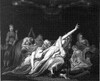
\includegraphics[keepaspectratio,width=\textwidth]{v7cfk63b-small.jpg}
  \captionart{DeathLooms}
  \label{fig:deathlooms}
\end{figure}
% Force float here
\clearpage{}
\chapter[Of Diseases and Melancholy]{Of Diseases in General, and of Melancholy; with a Digression of Anatomy}
{%_Man's Excellency, Fall, Miseries, Infirmities; The causes of them_.
\section[Man's Excellency, Fall, Miseries]{Man's Excellency, Fall, Miseries, Infirmities; The causes of them.}

\subsection{Man's Excellency.}
\lettrine[lines=4,findent=5pt,nindent=0pt]{M}{an} the most excellent and noble creature of the world, the principal and mighty work of God, wonder of Nature, 
as Zoroaster calls him; \li{audacis naturae miraculum}, the marvel of marvels\authormarginnote{820},
as Plato; the abridgment and epitome of the world\authormarginnote{821},
as \Pliny{}; microcosmus, a little world, a model of the world, sovereign lord of the earth\authormarginnote{822}, viceroy of the world, sole commander and governor of all the creatures in it; to whose empire they are subject in particular, and yield obedience; far surpassing all the rest, not in body only, but in soul; \authormarginnote{823}\li{imaginis imago}, \authormarginnote{824}created to God's own \authormarginnote{825}image, to that immortal and incorporeal substance, with all the faculties and powers belonging unto it; was at first pure, divine, perfect, happy, created after God in true holiness and righteousness\authormarginnote{826}; \li{Deo congruens}, free from all manner of infirmities, and put in Paradise, to know God, to praise and glorify him, to do his will, \li{Ut diis consimiles parturiat deos} (as an old poet saith) to propagate the church.

\subsection{Man's Fall and Misery.}
But this most noble creature, \li{Heu tristis, et lachrymosa commutatio} (one exclaims\authormarginnote{827}) O pitiful change! is fallen from that he was, and forfeited his estate, become \li{miserabilis homuncio}, a castaway, a caitiff, one of the most miserable creatures of the world, if he be considered in his own nature, an unregenerate man, and so much obscured by his fall that (some few relics excepted) he is inferior to a beast, \authormarginnote{828}Man in honour that understandeth not, is like unto beasts that perish, so David esteems him: a monster by stupend metamorphoses, \authorfootnote{829}a fox, a dog, a hog, what not? \li{Quantum mutatus ab illo?} How much altered from that he was; before blessed and happy, now miserable and accursed; \authorfootnote{830}He must eat his meat in sorrow, subject to death and all manner of infirmities, all kind of calamities.

\subsection{A Description of Melancholy.}
\authorfootnote{831}Great travail is created for all men, and an heavy yoke on the sons of Adam, from the day that they go out of their mother's womb, unto that day they return to the mother of all things. Namely, their thoughts, and fear of their hearts, and their imagination of things they wait for, and the day of death. From him that sitteth in the glorious throne, to him that sitteth beneath in the earth and ashes; from him that is clothed in blue silk and weareth a crown, to him that is clothed in simple linen. Wrath, envy, trouble, and unquietness, and fear of death, and rigour, and strife, and such things come to both man and beast, but sevenfold to the ungodly. All this befalls him in this life, and peradventure eternal misery in the life to come.

\subsection[The Impulsive Cause]{Impulsive Cause of Man's Misery and Infirmities.}
The impulsive cause of these miseries in man, this privation or destruction of God's image, the cause of death and diseases, of all temporal and eternal punishments, was the sin of our first parent Adam, \authorfootnote{832}in eating of the forbidden fruit, by the devil's instigation and allurement.
His disobedience, pride, ambition, intemperance, incredulity, curiosity; from whence proceeded original sin, and that general corruption of mankind, as from a fountain, flowed all bad inclinations and actual transgressions which cause our several calamities inflicted upon us for our sins.
And this belike is that which our fabulous poets have shadowed unto us in the tale of \authorfootnote{833} Pandora's box, which being opened through her curiosity, filled the world full of all manner of diseases.
It is not curiosity alone, but those other crying sins of ours, which pull these several plagues and miseries upon our heads.
For \li{Ubi peccatum, ibi procella}, as \Chrysostom{} well observes\authorfootnote{834}.
\authorfootnote{835}Fools by reason of their transgression, and because of their iniquities, are afflicted.
\authorfootnote{836}Fear cometh like sudden desolation, and destruction like a whirlwind, affliction and anguish, because they did not fear God.
\authorfootnote{837}Are you shaken with wars? as Cyprian well urgeth to Demetrius, are you molested with dearth and famine? is your health crushed with raging diseases? is mankind generally tormented with epidemical maladies? 'tis all for your sins, Hag. i. 9, 10; Amos i.; Jer. vii.
God is angry, punisheth and threateneth, because of their obstinacy and stubbornness, they will not turn unto him.
\authorfootnote{838}If the earth be barren then for want of rain, if dry and squalid, it yield no fruit, if your fountains be dried up, your wine, corn, and oil blasted, if the air be corrupted, and men troubled with diseases, 'tis by reason of their sins: which like the blood of Abel cry loud to heaven for vengeance, Lam. v. 15. That we have sinned, therefore our hearts are heavy, Isa. lix. 11, 12.
We roar like bears, and mourn like doves, and want health, \etc{} for our sins and trespasses.
But this we cannot endure to hear or to take notice of, Jer. ii. 30. We are smitten in vain and receive no correction; and cap. v. 3.
Thou hast stricken them, but they have not sorrowed; they have refused to receive correction; they have not returned.
Pestilence he hath sent, but they have not turned to him, Amos iv. \authorfootnote{839}Herod could not abide John Baptist, nor \authorfootnote{840}Domitian endure Apollonius to tell the causes of the plague at Ephesus, his injustice, incest, adultery, and the like.
To punish therefore this blindness and obstinacy of ours as a concomitant cause and principal agent, is God's just judgment in bringing these calamities upon us, to chastise us, I say, for our sins, and to satisfy God's wrath.
For the law requires obedience or punishment, as you may read at large, Deut. \rn{xxviii.} 15. If they will not obey the Lord, and keep his commandments and ordinances, then all these curses shall come upon them. \authorfootnote{841}Cursed in the town and in the field, \etc{}.
\authorfootnote{842}Cursed in the fruit of the body, \etc{}.
\authorfootnote{843}The Lord shall send thee trouble and shame, because of thy wickedness.
And a little after, \authorfootnote{844}The Lord shall smite thee with the botch of Egypt, and with emerods, and scab, and itch, and thou canst not be healed; \authorfootnote{845}with madness, blindness, and astonishing of heart.
This Paul seconds, Rom. ii. 9.
Tribulation and anguish on the soul of every man that doeth evil.
Or else these chastisements are inflicted upon us for our humiliation, to exercise and try our patience here in this life to bring us home, to make us to know God ourselves, to inform and teach us wisdom.
\authorfootnote{846}Therefore is my people gone into captivity, because they had no knowledge; therefore is the wrath of the Lord kindled against his people, and he hath stretched out his hand upon them.
He is desirous of our salvation.
\li{Nostrae salutis avidus}, saith Lemnius\authorfootnote{847}, and for that cause pulls us by the ear many times, to put us in mind of our duties: That they which erred might have understanding, (as Isaiah speaks \rn{xxix.} 24) and so to be reformed.
I am afflicted\authorfootnote{848}, and at the point of death, so David confesseth of himself, Psal. \rn{lxxxviii.} v. 15, v. 9.
Mine eyes are sorrowful through mine affliction: and that made him turn unto God.
Great Alexander in the midst of all his prosperity, by a company of parasites deified, and now made a god, when he saw one of his wounds bleed, remembered that he was but a man, and remitted of his pride.
\li{In morbo recolligit se animus}\authorlatintrans{849}, as \Pliny{} well perceived\authorfootnote{850}; In sickness the mind reflects upon itself, with judgment surveys itself, and abhors its former courses; insomuch that he concludes to his friend Marius,\authorfootnote{851} that it were the period of all philosophy, if we could so continue sound, or perform but a part of that which we promised to do, being sick.
Whoso is wise then, will consider these things, as David did (Psal. cxliv., verse last); and whatsoever fortune befall him, make use of it.
If he be in sorrow, need, sickness, or any other adversity, seriously to recount with himself, why this or that malady, misery, this or that incurable disease is inflicted upon him; it may be for his good, \authorfootnote{852}sic expedit as Peter said of his daughter's ague.
Bodily sickness is for his soul's health, periisset nisi periisset, had he not been visited, he had utterly perished; for \authorfootnote{853}the Lord correcteth him whom he loveth, even as a father doth his child in whom he delighteth.
If he be safe and sound on the other side, and free from all manner of infirmity; \authorfootnote{854}et cui Gratia, forma, valetudo contingat abunde Et mundus victus, non deficiente crumena.

And that he have grace, beauty, favour, health,
A cleanly diet, and abound in wealth.

Yet in the midst of his prosperity, let him remember that caveat of
Moses, \authorfootnote{855}Beware that he do not forget the Lord his God; that he be
not puffed up, but acknowledge them to be his good gifts and benefits,
and \authorfootnote{856}the more he hath, to be more thankful, (as Agapetianus
adviseth) and use them aright.

\cleartoleftpage{}
\newgeometry{noheadfoot=true}
\begin{figure}[p]
  \begingroup
  \centering
  
\includegraphics[keepaspectratio,width=0.95\textwidth]{caron-dionysius-converts-pagans-small.jpg}
  \captionart{DionysiusConvertsPagans}
  \label{fig:dionysiusconvertspagans}
\end{figure}
\restoregeometry

% Force float here
\clearpage{}
\subsection{Instrumental Causes of our Infirmities.}
Now the instrumental causes
of these our infirmities, are as diverse as the infirmities themselves;
stars, heavens, elements, \etc{}. And all those creatures which God hath
made, are armed against sinners. They were indeed once good in
themselves, and that they are now many of them pernicious unto us, is
not in their nature, but our corruption, which hath caused it. For from
the fall of our first parent Adam, they have been changed, the earth
accursed, the influence of stars, altered, the four elements, beasts,
birds, plants, are now ready to offend us. The principal things for the
use of man, are water, fire, iron, salt, meal, wheat, honey, milk, oil,
wine, clothing, good to the godly, to the sinners turned to evil,
Ecclus. \rn{xxxix.} 26. Fire, and hail, and famine, and dearth, all these
are created for vengeance, Ecclus. \rn{xxxix.} 29. The heavens threaten us
with their comets, stars, planets, with their great conjunctions,
eclipses, oppositions, quartiles, and such unfriendly aspects. The air
with his meteors, thunder and lightning, intemperate heat and cold,
mighty winds, tempests, unseasonable weather; from which proceed
dearth, famine, plague, and all sorts of epidemical diseases, consuming
infinite myriads of men. At Cairo in Egypt, every third year, (as it is
related by Boterus\authorfootnote{857}, and others) 300\thinspace{}000 die of the plague; and
200\thinspace{}000, in Constantinople, every fifth or seventh at the utmost. How
doth the earth terrify and oppress us with terrible earthquakes, which
are most frequent in China\authorfootnote{858}, Japan, and those eastern climes,
swallowing up sometimes six cities at once? How doth the water rage
with his inundations, irruptions, flinging down towns, cities,
villages, bridges, \etc{} besides shipwrecks; whole islands are sometimes
suddenly overwhelmed with all their inhabitants in Zealand\authorfootnote{859},
Holland, and many parts of the continent drowned, as the lake Erne
in Ireland?\authormarginnote{860} \li{Nihilque praeter arcium cadavera patenti cernimus
freto}\authorlatintrans{861.5}.\authormarginnote{861} In the fens of Friesland 1230, by reason of tempests, \authorfootnote{862}the
sea drowned \li{multa hominum millia, et jumenta sine numero}, all the
country almost, men and cattle in it. How doth the fire rage, that
merciless element, consuming in an instant whole cities? What town of
any antiquity or note hath not been once, again and again, by the fury
of this merciless element, defaced, ruinated, and left desolate? In a
word,
%
\begin{verse}
\textlatin{Ignis pepercit, unda mergit, aeris}\\*
\textlatin{Vis pestilentis aequori ereptum necat,}\\*
\textlatin{Bello superstes, tabidus morbo perit.}\authorfootnote{863}
\end{verse}
\translationrule
\begin{verse}
Whom fire spares, sea doth drown; whom sea,\\*
Pestilent air doth send to clay;\\*
Whom war 'scapes, sickness takes away.
\end{verse}

To descend to more particulars, how many creatures are at deadly feud
with men? Lions, wolves, bears, \etc{}. Some with hoofs, horns, tusks,
teeth, nails: How many noxious serpents and venomous creatures, ready
to offend us with stings, breath, sight, or quite kill us? How many
pernicious fishes, plants, gums, fruits, seeds, flowers, \etc{} could I
reckon up on a sudden, which by their very smell many of them, touch,
taste, cause some grievous malady, if not death itself? Some make
mention of a thousand several poisons: but these are but trifles in
respect. The greatest enemy to man, is man, who by the devil's
instigation is still ready to do mischief, his own executioner, a wolf,
a devil to himself, and others. We are all brethren in Christ\authorfootnote{864}, or
at least should be, members of one body, servants of one lord, and yet
no fiend can so torment, insult over, tyrannise, vex, as one man doth
another. Let me not fall therefore (saith David, when wars, plague,
famine were offered) into the hands of men, merciless and wicked men:
---\li{Vix sunt homines hoc nomine digni,
Quamque lupi, saevae plus feritatis habent}\authorfootnote{865}.

We can most part foresee these epidemical diseases, and likely avoid
them; Dearths, tempests, plagues, our astrologers foretell us;
Earthquakes, inundations, ruins of houses, consuming fires, come by
little and little, or make some noise beforehand; but the knaveries,
impostures, injuries and villainies of men no art can avoid. We can
keep our professed enemies from our cities, by gates, walls and towers,
defend ourselves from thieves and robbers by watchfulness and weapons;
but this malice of men, and their pernicious endeavours, no caution can
divert, no vigilancy foresee, we have so many secret plots and devices
to mischief one another.

Sometimes by the devil's help as magicians, witches\authorfootnote{866}: sometimes by
impostures, mixtures, poisons, stratagems, single combats, wars, we
hack and hew, as if we were ad internecionem nati, like Cadmus'
soldiers born to consume one another. 'Tis an ordinary thing to read of
a hundred and two hundred thousand men slain in a battle. Besides all
manner of tortures, brazen bulls, racks, wheels, strappadoes, guns,
engines, \etc{}. Ad unum corpus humanum supplicia plura, quam membra\authormarginnote{867}:
We have invented more torturing instruments, than there be several
members in a man's body, as Cyprian well observes. To come nearer yet,
our own parents by their offences, indiscretion and intemperance, are
our mortal enemies. The fathers have eaten sour grapes\authorfootnote{868}, and the
children's teeth are set on edge. They cause our grief many times, and
put upon us hereditary diseases, inevitable infirmities: they torment
us, and we are ready to injure our posterity;
---\li{mox daturi progeniem vitiosiorem}\authorfootnote{869}.

And yet with crimes to us unknown,
Our sons shall mark the coming age their own;

and the latter end of the world, as Paul foretold\authorfootnote{870}, is still like
to be the worst. We are thus bad by nature, bad by kind, but far worse
by art, every man the greatest enemy unto himself. We study many times
to undo ourselves, abusing those good gifts which God hath bestowed
upon us, health, wealth, strength, wit, learning, art, memory to our
own destruction, \li{Perditio tua ex te}\authorlatintrans{871.5}.\authormarginnote{871} As Judas Maccabeus
killed Apollonius with his own weapons\authorfootnote{872}, we arm ourselves to our own
overthrows; and use reason, art, judgment, all that should help us, as
so many instruments to undo us. Hector gave Ajax a sword, which so long
as he fought against enemies, served for his help and defence; but
after he began to hurt harmless creatures with it, turned to his own
hurtless bowels. Those excellent means God hath bestowed on us, well
employed, cannot but much avail us; but if otherwise perverted, they
ruin and confound us: and so by reason of our indiscretion and weakness
they commonly do, we have too many instances. This St. \Austin{}
acknowledgeth of himself in his humble confessions, promptness of wit,
memory, eloquence, they were God's good gifts, but he did not use them
to his glory. If you will particularly know how, and by what means,
consult physicians, and they will tell you, that it is in offending in
some of those six non-natural things, of which I shall \authorfootnote{873}dilate more
at large; they are the causes of our infirmities, our surfeiting, and
drunkenness, our immoderate insatiable lust, and prodigious riot.

\li{Plures crapula, quam gladius}, is a true saying, the board consumes more
than the sword. Our intemperance it is, that pulls so many several
incurable diseases upon our heads, that hastens \authorfootnote{874}old age, perverts
our temperature, and brings upon us sudden death. And last of all, that
which crucifies us most, is our own folly, madness (quos Jupiter
perdit, dementat; by subtraction of his assisting grace God permits it)
weakness, want of government, our facility and proneness in yielding to
several lusts, in giving way to every passion and perturbation of the
mind: by which means we metamorphose ourselves and degenerate into
beasts. All which that prince of \authorfootnote{875}poets observed of Agamemnon, that
when he was well pleased, and could moderate his passion, he was-os
oculosque Jovi par: like Jupiter in feature, Mars in valour, Pallas in
wisdom, another god; but when he became angry, he was a lion, a tiger,
a dog, \etc{}, there appeared no sign or likeness of Jupiter in him; so
we, as long as we are ruled by reason, correct our inordinate appetite,
and conform ourselves to God's word, are as so many saints: but if we
give reins to lust, anger, ambition, pride, and follow our own ways, we
degenerate into beasts, transform ourselves, overthrow our
constitutions, \authorfootnote{876}provoke God to anger, and heap upon us this of
melancholy, and all kinds of incurable diseases, as a just and deserved
punishment of our sins.

\section{The Definition, Number, Division of Diseases.}

\lettrine{W}{hat} a disease is, almost every physician defines. \authorfootnote{877}Fernelius
calleth it an affection of the body contrary to nature. \authorfootnote{878}Fuschius
and Crato, an hindrance, hurt, or alteration of any action of the body,
or part of it. \authorfootnote{879}Tholosanus, a dissolution of that league which is
between body and soul, and a perturbation of it; as health the
perfection, and makes to the preservation of it. \li{Labeo in
Agellius},\authormarginnote{880} an ill habit of the body, opposite to nature, hindering the
use of it. Others otherwise, all to this effect.

\subsection{Number of Diseases.}
How many diseases there are, is a question not yet determined;
\authorfootnote{881}\Pliny{} reckons up 300 from the crown of the head to the sole
of the foot: elsewhere he saith, \lit{their number is infinite}{morborum
infinita multitudo}. Howsoever it was in those times, it boots not; in our days
I am sure the number is much augmented:
%
\authormarginnote{882}\begin{latin}
\begin{quote}
---macies, et nova febrium
Terris incubit cohors.
\end{quote}
\end{latin}
\translationrule
\begin{quote}%\authorlatintrans{882.5}
Emaciation, and a new cohort of fevers broods over the earth.
\end{quote}

For besides many epidemical diseases unheard of, and altogether unknown
to Galen and Hippocrates, as scorbutum, small-pox, plica, sweating
sickness, morbus Gallicus, \etc{}, we have many proper and peculiar almost
to every part.

\subsection{No man free from some Disease or other.}
No man amongst us so sound, of so good a constitution, that hath not some impediment of body or
mind. \li{Quisque suos patimur manes}, we have all our infirmities, first or
last, more or less. There will be peradventure in an age, or one of a
thousand, like Zenophilus the musician in \authorfootnote{883}\Pliny{}, that may happily
live 105 years without any manner of impediment; a Pollio Romulus, that
can preserve himself \authorfootnote{884}with wine and oil; a man as fortunate as Q.
Metellus, of whom Valerius so much brags; a man as healthy as Otto
Herwardus, a senator of Augsburg in Germany, whom \authorfootnote{885}Leovitius the
astrologer brings in for an example and instance of certainty in his
art; who because he had the significators in his geniture fortunate,
and free from the hostile aspects of Saturn and Mars, being a very cold
man, \authorfootnote{886}could not remember that ever he was sick. \authorfootnote{887}Paracelsus may
brag that he could make a man live 400 years or more, if he might bring
him up from his infancy, and diet him as he list; and some physicians
hold, that there is no certain period of man's life; but it may still
by temperance and physic be prolonged. We find in the meantime, by
common experience, that no man can escape, but that of Hesiod is
true\authorfootnote{888}:
%
\begin{foreigndisplayquote}{greek}%
Πλείη μὲν γὰρ γαῖα κακῶν, πλειη δὲ θάλασσα,
Νοῦσοιδ' ἄνθρωποι ἐιν ἐφ' ἡμέρη, ἠδ' ἐπὶ νυκτὶ
Ἁυτοματοι φοιτῶσι.%
\end{foreigndisplayquote}%
\translationrule%
\begin{quote}%
Th' earth's full of maladies, and full the sea,
Which set upon us both by night and day.
\end{quote}%

\subsection{Division of Diseases.}
If you require a more exact division of these
ordinary diseases which are incident to men, I refer you to physicians;
\authorfootnote{889}they will tell you of acute and chronic, first and secondary,
lethals, salutares, errant, fixed, simple, compound, connexed, or
consequent, belonging to parts or the whole, in habit, or in
disposition, \etc{}. My division at this time (as most befitting my
purpose) shall be into those of the body and mind. For them of the
body, a brief catalogue of which Fuschius hath made, Institut. lib. 3,
sect. 1, cap. 11. I refer you to the voluminous tomes of Galen,
Areteus, Rhasis, \Avicenna{}, Alexander, Paulus Aetius, Gordonerius: and
those exact Neoterics, Savanarola, Capivaccius, Donatus Altomarus,
Hercules de Saxonia, Mercurialis, Victorius Faventinus, Wecker, Piso,
\etc{}, that have methodically and elaborately written of them all. Those
of the mind and head I will briefly handle, and apart.

\section{Division of the Diseases of the Head.}

\lettrine{T}{hese} diseases of the mind, forasmuch as they have their chief seat and
organs in the head, which are commonly repeated amongst the diseases of
the head which are diverse, and vary much according to their site. For
in the head, as there be several parts, so there be diverse grievances,
which according to that division of \authorfootnote{890}Heurnius, (which he takes out
of Arculanus) are inward or outward (to omit all others which pertain
to eyes and ears, nostrils, gums, teeth, mouth, palate, tongue, weezle,
chops, face, \etc{}) belonging properly to the brain, as baldness, falling
of hair, furfur, lice, \etc{}. \authorfootnote{891}Inward belonging to the skins next to
the brain, called \emph{dura} and \emph{pia mater}, as all headaches, \etc{}, or to
the ventricles, caules, kells, tunicles, creeks, and parts of it, and
their passions, as caro, vertigo, incubus, apoplexy, falling sickness.

The diseases of the nerves, cramps, stupor, convulsion, tremor, palsy:
or belonging to the excrements of the brain, catarrhs, sneezing,
rheums, distillations: or else those that pertain to the substance of
the brain itself, in which are conceived frenzy, lethargy, melancholy,
madness, weak memory, sopor, or Coma Vigilia et vigil Coma. Out of
these again I will single such as properly belong to the phantasy, or
imagination, or reason itself, which Laurentius calls\authorfootnote{892} the disease
of the mind; and Hildesheim, \latininlinetrans{diseases of the imagination, or of injured reason}{morbos imaginationis, aut rationis laesae},
 which are three or four in number, frenzy, madness, melancholy, dotage, and their kinds:
as hydrophobia, lycanthropia, \latininlinetrans{St. Vitus's dance, possession of devils}{Chorus sancti viti, morbi daemoniaci}, which I will briefly touch
and point at, insisting especially in this of melancholy, as more
eminent than the rest, and that through all his kinds, causes,
symptoms, prognostics, cures: as Lonicerus hath done de apoplexia, and
many other of such particular diseases. Not that I find fault with
those which have written of this subject before, as Jason Pratensis,
Laurentius, Montaltus, T. Bright, \etc{}, they have done very well in
their several kinds and methods; yet that which one omits, another may
haply see; that which one contracts, another may enlarge. To conclude
with \authorfootnote{893}Scribanius, that which they had neglected, or perfunctorily
handled, we may more thoroughly examine; that which is obscurely
delivered in them, may be perspicuously dilated and amplified by us:
and so made more familiar and easy for every man's capacity, and the
common good, which is the chief end of my discourse.

\section[Madness]{Dotage, Frenzy, Madness, Hydrophobia, Lycanthropia, Chorus sancti Viti, Extasis.}
\begin{figure}[H]
  \begingroup
  \centering
  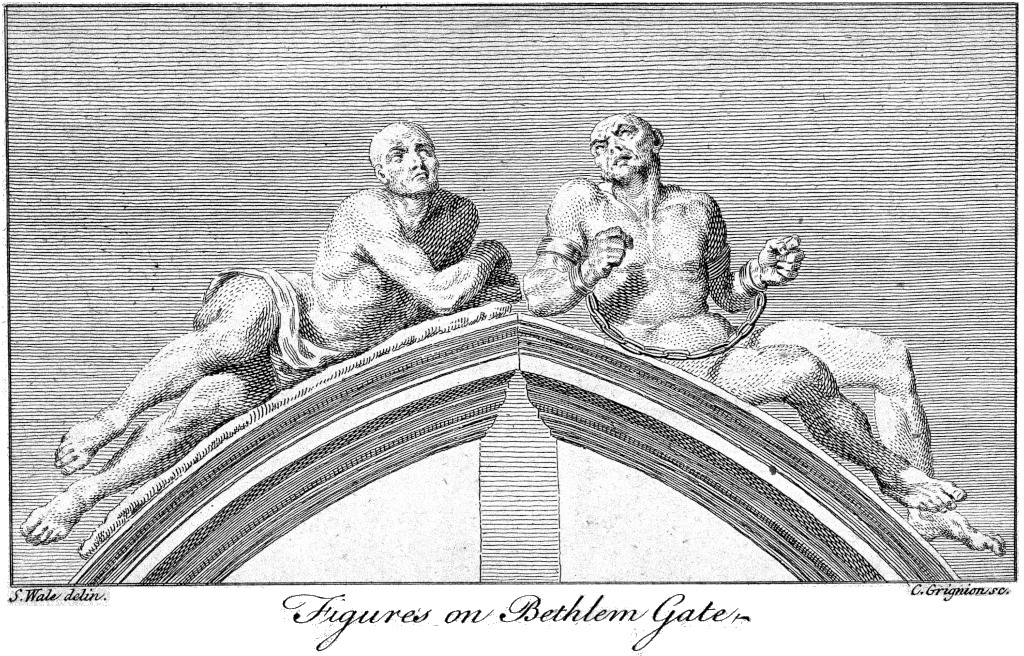
\includegraphics[keepaspectratio,width=\textwidth]{tmczmfhz-small.jpg}
  \captionart{Madness}
  \label{fig:madness}
\end{figure}
\subsection{Delirium, Dotage.}
\lettrine{D}{otage}, fatuity, or folly, is a common name to all
the following species, as some will have it. \authorfootnote{894}Laurentius and \authorfootnote{895}
Altomarus comprehended madness, melancholy, and the rest under this
name, and call it the summum genus of them all. If it be distinguished
from them, it is natural or ingenite, which comes by some defect of the
organs, and overmuch brain, as we see in our common fools; and is for
the most part intended or remitted in particular men, and thereupon
some are wiser than others: or else it is acquisite, an appendix or
symptom of some other disease, which comes or goes; or if it continue,
a sign of melancholy itself.

\subsection{Frenzy.}
\emph{Phrenitis}, which the Greeks derive from the word \textgreek{φρην}, is
a disease of the mind, with a continual madness or dotage, which hath
an acute fever annexed, or else an inflammation of the brain, or the
membranes or kells of it, with an acute fever, which causeth madness
and dotage. It differs from melancholy and madness, because their
dotage is without an ague: this continual, with waking, or memory
decayed, \etc{}. Melancholy is most part silent, this clamorous; and many
such like differences are assigned by physicians.

\subsection{Madness.}
Madness, frenzy, and melancholy are confounded by Celsus,
and many writers; others leave out frenzy, and make madness and
melancholy but one disease, which \authorfootnote{896}Jason Pratensis especially
labours, and that they differ only \li{secundam majus} or minus, in quantity
alone, the one being a degree to the other, and both proceeding from
one cause. They differ intenso et remisso gradu, saith \authorfootnote{897}Gordonius,
as the humour is intended or remitted. Of the same mind is
\authorfootnote{898}Areteus, Alexander Tertullianus, Guianerius, Savanarola, Heurnius;
and Galen himself writes promiscuously of them both by reason of their
affinity: but most of our neoterics do handle them apart, whom I will
follow in this treatise. Madness is therefore defined to be a vehement
dotage; or raving without a fever, far more violent than melancholy,
full of anger and clamour, horrible looks, actions, gestures, troubling
the patients with far greater vehemency both of body and mind, without
all fear and sorrow, with such impetuous force and boldness, that
sometimes three or four men cannot hold them. Differing only in this
from frenzy, that it is without a fever, and their memory is most part
better. It hath the same causes as the other, as choler adust, and
blood incensed, brains inflamed, \etc{}. \authorfootnote{899}Fracastorius adds, a due
time, and full age to this definition, to distinguish it from children,
and will have it confirmed impotency, to separate it from such as
accidentally come and go again, as by taking henbane, nightshade, wine,
\etc{}. Of this fury there be diverse kinds; ecstasy\authormarginnote{900}, which is familiar
with some persons, as Cardan saith of himself, he could be in one when
he list; in which the Indian priests deliver their oracles, and the
witches in Lapland, as Olaus Magnus writeth, \textlatin{l. 3, cap. 18. Extasi
omnia praedicere}, answer all questions in an ecstasis you will ask;
what your friends do, where they are, how they fare, \etc{}. The other
species of this fury are enthusiasms, revelations, and visions, so
often mentioned by Gregory and Bede in their works; obsession or
possession of devils, sibylline prophets, and poetical furies; such as
come by eating noxious herbs, tarantulas stinging, \etc{}, which some
reduce to this. The most known are these, lycanthropia, hydrophobia,
\textlatin{chorus sancti Viti}.

\cleartoleftpage{}
\begin{figure}[p]
  \begingroup
  \centering
  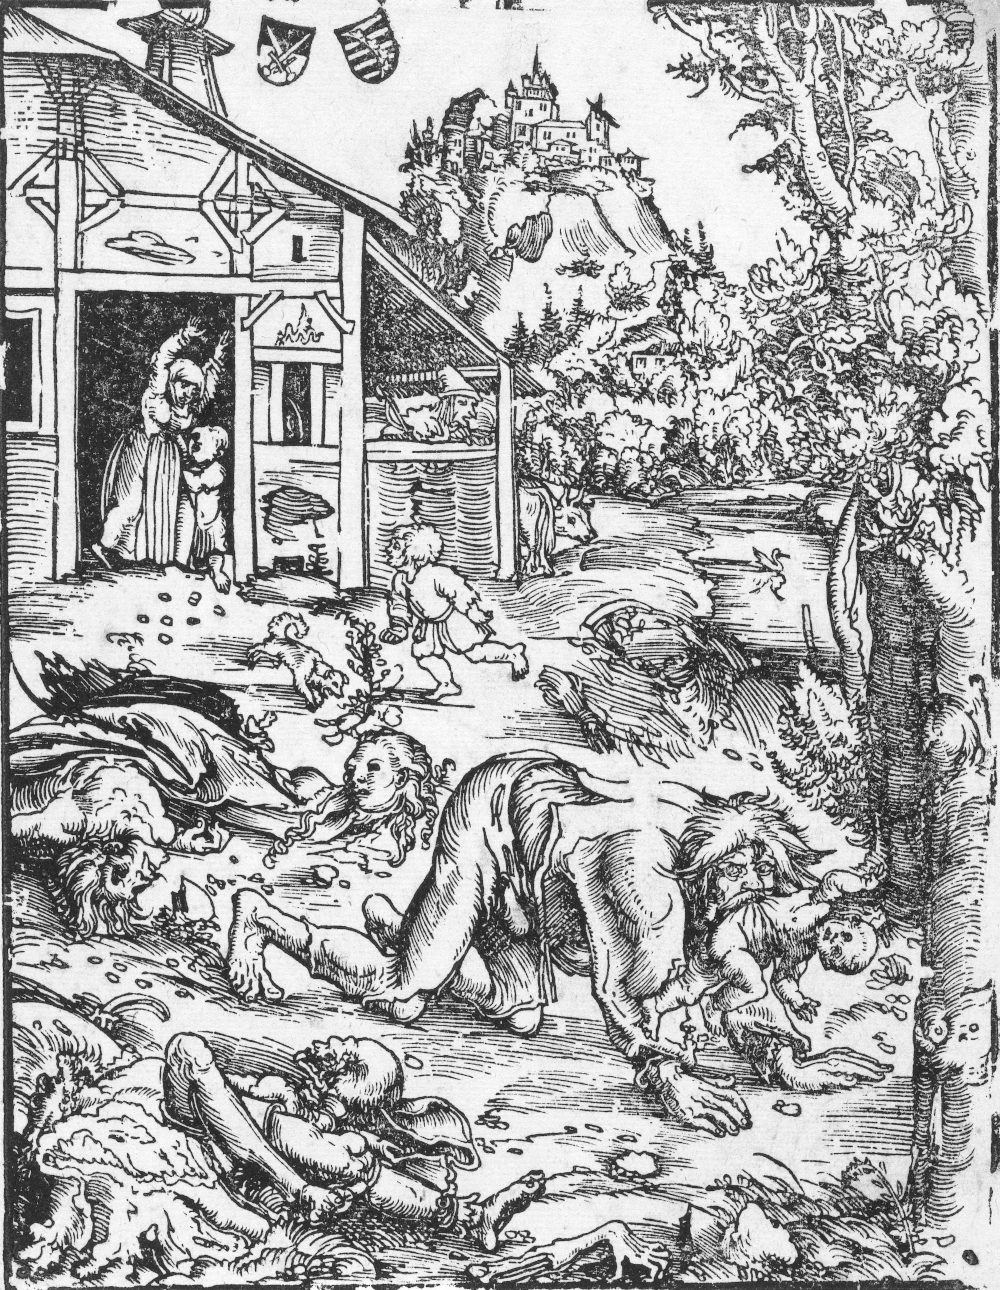
\includegraphics[keepaspectratio,width=\textwidth]{Werewolf-with-bodies-small.jpg}
  \captionart{Werewolf}
  \label{fig:werewolf}
\end{figure}

% Force float here
\clearpage{}
\subsection{Lycanthropia.}
Lycanthropia, which \Avicenna{} calls \emph{cucubuth}, others
\emph{lupinam insaniam}, or wolf-madness, when men run howling about graves
and fields in the night, and will not be persuaded but that they are
wolves, or some such beasts. \authorfootnote{901}Aetius and \authorfootnote{902}Paulus call it a kind
of melancholy; but I should rather refer it to madness, as most do.

Some make a doubt of it whether there be any such disease. \authorfootnote{903}Donat
ab Altomari saith, that he saw two of them in his time: \authorfootnote{904}Wierus
tells a story of such a one at Padua 1541, that would not believe to
the contrary, but that he was a wolf. He hath another instance of a
Spaniard, who thought himself a bear; \authorfootnote{905}Forrestus confirms as much
by many examples; one amongst the rest of which he was an eyewitness,
at Alcmaer in Holland, a poor husbandman that still hunted about
graves, and kept in churchyards, of a pale, black, ugly, and fearful
look. Such belike, or little better, were king Praetus' \authorfootnote{906}daughters,
that thought themselves kine. And Nebuchadnezzar in Daniel, as some
interpreters hold, was only troubled with this kind of madness. This
disease perhaps gave occasion to that bold assertion of \authorfootnote{907}\Pliny{},
some men were turned into wolves in his time, and from wolves to men
again: and to that fable of Pausanias, of a man that was ten years a
wolf, and afterwards turned to his former shape: to \authorfootnote{908}\Ovid's tale of
Lycaon, \etc{}. He that is desirous to hear of this disease, or more
examples, let him read \Austin{} in his 18th book de Civitate Dei, cap. 5.
Mizaldus, cent. 5. 77. Sckenkius, lib. 1. Hildesheim, spicel. 2. de
Mania. Forrestus lib. 10. de morbis cerebri. Olaus Magnus, Vincentius
Bellavicensis, spec. met. lib. 31. c. 122. Pierius, Bodine, Zuinger,
Zeilger, Peucer, Wierus, Spranger, \etc{}. This malady, saith \Avicenna{},
troubleth men most in February, and is nowadays frequent in Bohemia and
Hungary, according to \authorfootnote{909}Heurnius. Scheretzius will have it common in
Livonia. They lie hid most part all day, and go abroad in the night,
barking, howling, at graves and deserts; \authorfootnote{910}they have usually hollow
eyes, scabbed legs and thighs, very dry and pale, \authorfootnote{911}saith Altomarus;
he gives a reason there of all the symptoms, and sets down a brief cure
of them.

\emph{Hydrophobia} is a kind of madness, well known in every village, which
comes by the biting of a mad dog, or scratching, saith \authorfootnote{912}Aurelianus;
touching, or smelling alone sometimes as Sckenkius proves\authorfootnote{913}, and is
incident to many other creatures as well as men: so called because the
parties affected cannot endure the sight of water, or any liquor,
supposing still they see a mad dog in it. And which is more wonderful;
though they be very dry, (as in this malady they are) they will rather
die than drink: \authorfootnote{914}de Venenis Caelius Aurelianus, an ancient writer,
makes a doubt whether this Hydrophobia be a passion of the body or the
mind. The part affected is the brain: the cause, poison that comes from
the mad dog, which is so hot and dry, that it consumes all the moisture
in the body. \authorfootnote{915} Hildesheim relates of some that died so mad; and
being cut up, had no water, scarce blood, or any moisture left in them.

To such as are so affected, the fear of water begins at fourteen days
after they are bitten, to some again not till forty or sixty days
after: commonly saith Heurnius, they begin to rave, fly water and
glasses, to look red, and swell in the face, about twenty days after
(if some remedy be not taken in the meantime) to lie awake, to be
pensive, sad, to see strange visions, to bark and howl, to fall into a
swoon, and oftentimes fits of the falling sickness. \authorfootnote{916} Some say,
little things like whelps will be seen in their urine. If any of these
signs appear, they are past recovery. Many times these symptoms will
not appear till six or seven months after, saith \authorfootnote{917}Codronchus; and
sometimes not till seven or eight years, as Guianerius; twelve as
Albertus; six or eight months after, as Galen holds. Baldus the great
lawyer died of it: an Augustine friar, and a woman in Delft, that were
\authorfootnote{918}Forrestus' patients, were miserably consumed with it. The common
cure in the country (for such at least as dwell near the seaside) is to
duck them over head and ears in sea water; some use charms: every good
wife can prescribe medicines. But the best cure to be had in such
cases, is from the most approved physicians; they that will read of
them, may consult with Dioscorides, lib. 6. c. 37, Heurnius,
Hildesheim, Capivaccius, Forrestus, Sckenkius and before all others
Codronchus an Italian, who hath lately written two exquisite books on
the subject.

\li{Chorus sancti Viti}, or St. Vitus's dance; the lascivious dance, \authorfootnote{919}
Paracelsus calls it, because they that are taken from it, can do
nothing but dance till they be dead, or cured. It is so called, for
that the parties so troubled were wont to go to St. Vitus for help, and
after they had danced there awhile, they were \authorfootnote{920}certainly freed.
'Tis strange to hear how long they will dance, and in what manner, over
stools, forms, tables; even great bellied women sometimes (and yet
never hurt their children) will dance so long that they can stir
neither hand nor foot, but seem to be quite dead. One in red clothes
they cannot abide. Music above all things they love, and therefore
magistrates in Germany will hire musicians to play to them, and some
lusty sturdy companions to dance with them. This disease hath been very
common in Germany, as appears by those relations of \authorfootnote{921}Sckenkius, and
Paracelsus in his book of Madness, who brags how many several persons
he hath cured of it. Felix Plateras de mentis alienat. cap. 3, reports
of a woman in Basil whom he saw, that danced a whole month together.
The Arabians call it a kind of palsy. Bodine in his 5th book de Repub.
cap. 1, speaks of this infirmity; Monavius in his last epistle to
Scoltizius, and in another to Dudithus, where you may read more of it.
The last kind of madness or melancholy, is that demoniacal (if I may so
call it) obsession or possession of devils, which Platerus and others
would have to be preternatural: stupend things are said of them, their
actions, gestures, contortions, fasting, prophesying, speaking
languages they were never taught, \etc{}. Many strange stories are related
of them, which because some will not allow, (for Deacon and Darrel have
written large volumes on this subject pro and con.) I voluntarily omit.
\authorfootnote{922}Fuschius, Institut. lib. 3. sec. 1. cap. 11, Felix Plater,
\authorfootnote{923}Laurentius, add to these another fury that proceeds from love, and
another from study, another divine or religious fury; but these more
properly belong to melancholy; of all which I will speak \authorfootnote{924}apart,
intending to write a whole book of them.

\cleartoleftpage{}
\begin{figure}[p]
  \begingroup
  \centering
  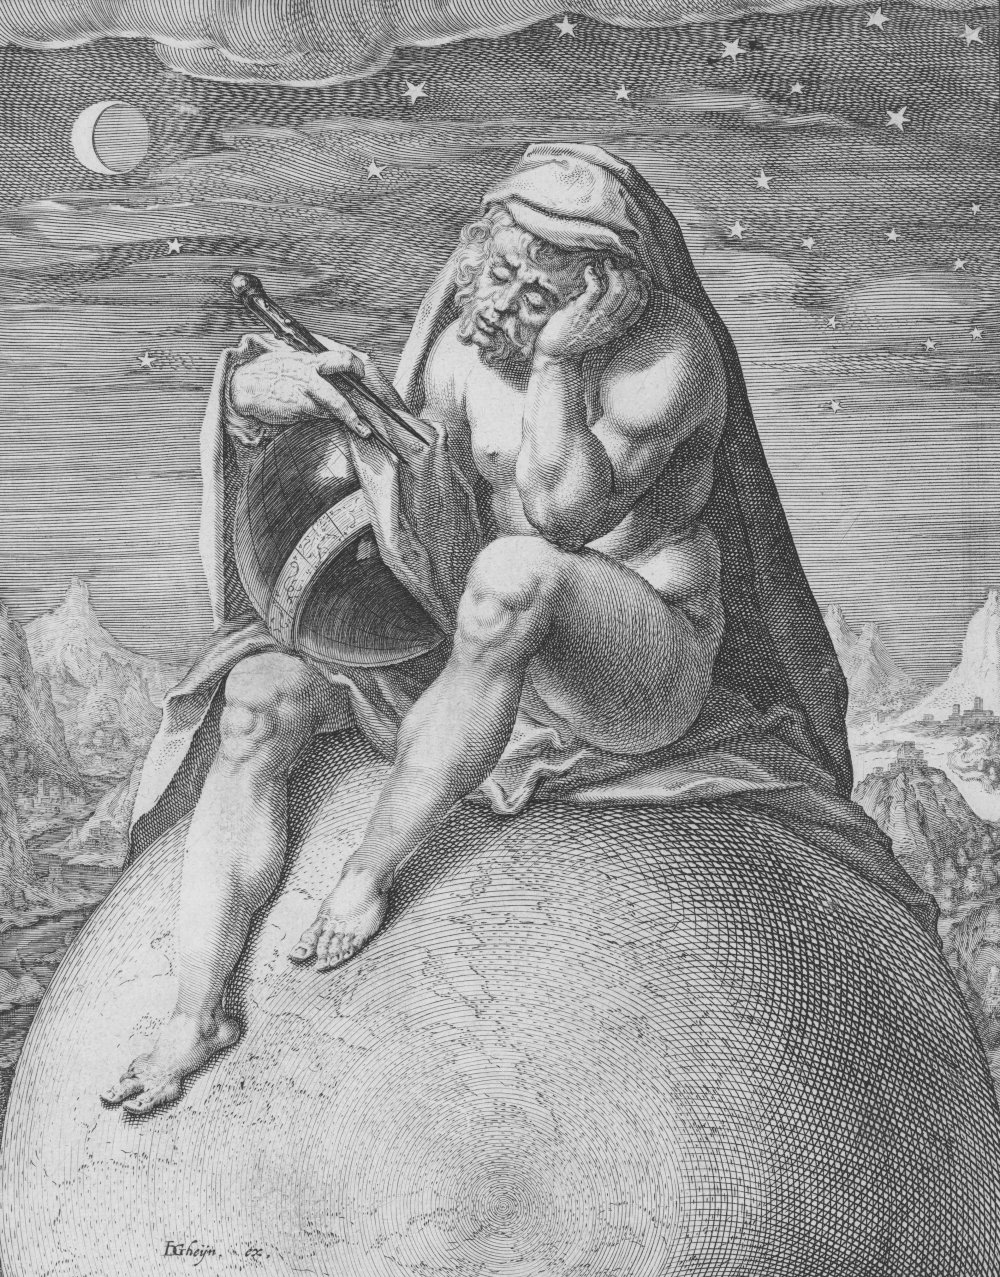
\includegraphics[keepaspectratio,width=\textwidth]{MelancholicTemperament-small.jpg}
  \captionart{MelancholicTemperament}
  \label{fig:melancholictemperament}
\end{figure}

% Force float here
\clearpage{}
\thispagestyle{titleontop}

\section[Melancholic Disposition]{Melancholy in Disposition, improperly so called, Equivocations.}
\lettrine{M}{elancholy}, the subject of our present discourse, is either in
disposition or habit. In disposition, is that transitory melancholy
which goes and comes upon every small occasion of sorrow, need,
sickness, trouble, fear, grief, passion, or perturbation of the mind,
any manner of care, discontent, or thought, which causeth anguish,
dullness, heaviness and vexation of spirit, any ways opposite to
pleasure, mirth, joy, delight, causing frowardness in us, or a dislike.
In which equivocal and improper sense, we call him melancholy that is
dull, sad, sour, lumpish, ill disposed, solitary, any way moved, or
displeased. And from these melancholy dispositions, \authorfootnote{925}no man living
is free, no stoic, none so wise, none so happy, none so patient, so
generous, so godly, so divine, that can vindicate himself; so well
composed, but more or less, some time or other he feels the smart of
it. Melancholy in this sense is the character of mortality. \authorfootnote{926}Man
that is born of a woman, is of short continuance, and full of trouble.
Zeno, Cato, Socrates himself, whom \authorfootnote{927}Aelian so highly commends for a
moderate temper, that nothing could disturb him, but going out, and
coming in, still Socrates kept the same serenity of countenance, what
misery soever befell him, (if we may believe Plato his disciple) was
much tormented with it. Q. Metellus, in whom \authorfootnote{928}Valerius gives
instance of all happiness, the most fortunate man then living, born in
that most flourishing city of Rome, of noble parentage, a proper man of
person, well qualified, healthful, rich, honourable, a senator, a
consul, happy in his wife, happy in his children, \etc{} yet this man was
not void of melancholy, he had his share of sorrow. \authorfootnote{929}Polycrates
Samius, that flung his ring into the sea, because he would participate
of discontent with others, and had it miraculously restored to him
again shortly after, by a fish taken as he angled, was not free from
melancholy dispositions. No man can cure himself; the very gods had
bitter pangs, and frequent passions, as their own \authorfootnote{930}poets put upon
them. In general, \authorfootnote{931}as the heaven, so is our life, sometimes fair,
sometimes overcast, tempestuous, and serene; as in a rose, flowers and
prickles; in the year itself, a temperate summer sometimes, a hard
winter, a drought, and then again pleasant showers: so is our life
intermixed with joys, hopes, fears, sorrows, calumnies: \lit{there is a succession of pleasure and pain}{Invicem cedunt dolor et voluptas}.

\authorfootnote{932}---\li{medio de fonte leporum
Surgit amari aliquid, in ipsis floribus angat}.

Even in the midst of laughing there is sorrow, (as Solomon holds\authorfootnote{933}):
even in the midst of all our feasting and jollity, as \Austin{}
infers\authorfootnote{934} in his Com. on the 41st Psalm, there is grief and discontent.
Inter delicias semper aliquid saevi nos strangulat, for a pint of honey
thou shalt here likely find a gallon of gall, for a dram of pleasure a
pound of pain, for an inch of mirth an ell of moan; as ivy doth an oak,
these miseries encompass our life. And it is most absurd and ridiculous
for any mortal man to look for a perpetual tenure of happiness in his
life. Nothing so prosperous and pleasant, but it hath \authorfootnote{935}some
bitterness in it, some complaining, some grudging; it is all
\marginnote{\scriptsize{}bittersweet}\textgreek{γλυκύπικρον}, a mixed passion,
and like a chequer table black and white: men, families, cities, have their falls and wanes; now trines,
sextiles, then quartiles and oppositions. We are not here as those
angels, celestial powers and bodies, sun and moon, to finish our course
without all offence, with such constancy, to continue for so many ages:
but subject to infirmities, miseries, interrupted, tossed and tumbled
up and down, carried about with every small blast, often molested and
disquieted upon each slender occasion, \authorfootnote{936}uncertain, brittle, and so
is all that we trust unto. \authorfootnote{937} And he that knows not this is not
armed to endure it, is not fit to live in this world (as one condoles
our time), he knows not the condition of it, where with a reciprocalty,
pleasure and pain are still united, and succeed one another in a ring.
\li{Exi e mundo}, get thee gone hence if thou canst not brook it; there is
no way to avoid it, but to arm thyself with patience, with magnanimity,
to \authorfootnote{938}oppose thyself unto it, to suffer affliction as a good soldier
of Christ; as Paul adviseth\authorfootnote{939} constantly to bear it. But forasmuch
as so few can embrace this good council of his, or use it aright, but
rather as so many brute beasts give away to their passion, voluntary
subject and precipitate themselves into a labyrinth of cares, woes,
miseries, and suffer their souls to be overcome by them, cannot arm
themselves with that patience as they ought to do, it falleth out
oftentimes that these dispositions become habits, and many affects
contemned (as \Seneca notes\authorfootnote{940}) make a disease. Even as one
distillation, not yet grown to custom, makes a cough; but continual and
inveterate causeth a consumption of the lungs; so do these our
melancholy provocations: and according as the humour itself is
intended, or remitted in men, as their temperature of body, or rational
soul is better able to make resistance; so are they more or less
affected. For that which is but a flea-biting to one, causeth
insufferable torment to another; and which one by his singular
moderation, and well-composed carriage can happily overcome, a second
is no whit able to sustain, but upon every small occasion of
misconceived abuse, injury, grief, disgrace, loss, cross, humour, \etc{}
(if solitary, or idle) yields so far to passion, that his complexion is
altered, his digestion hindered, his sleep gone, his spirits obscured,
and his heart heavy, his hypochondries misaffected; wind, crudity, on a
sudden overtake him, and he himself overcome with melancholy. As it is
with a man imprisoned for debt, if once in the gaol, every creditor
will bring his action against him, and there likely hold him. If any
discontent seize upon a patient, in an instant all other perturbations
(\li{for-qua data porta ruunt}) will set upon him, and then like a lame dog
or broken-winged goose he droops and pines away, and is brought at last
to that ill habit or malady of melancholy itself. So that as the
philosophers make \authorfootnote{941}eight degrees of heat and cold, we may make
eighty-eight of melancholy, as the parts affected are diversely seized
with it, or have been plunged more or less into this infernal gulf, or
waded deeper into it. But all these melancholy fits, howsoever pleasing
at first, or displeasing, violent and tyrannizing over those whom they
seize on for the time; yet these fits I say, or men affected, are but
improperly so called, because they continue not, but come and go, as by
some objects they aye moved. This melancholy of which we are to treat,
is a habit, \li{mosbus sonticus}, or \li{chronicus}, a chronic or continuate
disease, a settled humour, as Aurelianus\authorfootnote{942} and others\authorfootnote{943} call it,
not errant, but fixed; and as it was long increasing, so now being
(pleasant, or painful) grown to an habit, it will hardly be removed.

%SECT. I. MEMB. II.

%SECT. I. MEMB. II. SUBSECT. I.-_Digression of Anatomy_.
\section{Digression of Anatomy.}

\lettrine{B}{efore} I proceed to define the disease of melancholy, what it is, or to
discourse farther of it, I hold it not impertinent to make a brief
digression of the anatomy of the body and faculties of the soul, for
the better understanding of that which is to follow; because many hard
words will often occur, as mirach, hypocondries, emerods, \etc{},
imagination, reason, humours, spirits, vital, natural, animal, nerves,
veins, arteries, chylus, pituita; which by the vulgar will not so
easily be perceived, what they are, how cited, and to what end they
serve. And besides, it may peradventure give occasion to some men to
examine more accurately, search further into this most excellent
subject, and thereupon with that royal \authorfootnote{944}prophet to praise God, (for
a man is fearfully and wonderfully made, and curiously wrought) that
have time and leisure enough, and are sufficiently informed in all
other worldly businesses, as to make a good bargain, buy and sell, to
keep and make choice of a fair hawk, hound, horse, \etc{}. But for such
matters as concern the knowledge of themselves, they are wholly
ignorant and careless; they know not what this body and soul are, how
combined, of what parts and faculties they consist, or how a man
differs from a dog. And what can be more ignominious and filthy (as
\authorfootnote{945}Melancthon well inveighs) than for a man not to know the structure
and composition of his own body, especially since the knowledge of it
tends so much to the preservation, of his health, and information of
his manners? To stir them up therefore to this study, to peruse those
elaborate works of \authorfootnote{946}Galen, Bauhines, Plater, Vesalius, Falopius,
Laurentius, Remelinus, \etc{}, which have written copiously in Latin; or
that which some of our industrious countrymen have done in our mother
tongue, not long since, as that translation of \authorfootnote{947}Columbus and \authorfootnote{948}
Microcosmographia, in thirteen books, I have made this brief
digression. Also because \authorfootnote{949}Wecker, \authorfootnote{950}Melancthon, \authorfootnote{951}Fernelius,
\authorfootnote{952} Fuschius, and those tedious Tracts de Anima (which have more
compendiously handled and written of this matter) are not at all times
ready to be had, to give them some small taste, or notice of the rest,
let this epitome suffice.

%SECT. I. MEMB. II. SUBSECT. II.-_Division of the Body, Humours, Spirits_.
\section[Division of the Body]{Division of the Body, Humours, Spirits.}

\lettrine{O}{f} the parts of the body there may be many divisions: the most approved
is that of \authorfootnote{953}Laurentius, out of Hippocrates: which is, into parts
contained, or containing. Contained, are either humours or spirits.
\subsection{Humours.}
A humour is a liquid or fluent part of the body,
comprehended in it, for the preservation of it; and is either innate or
born with us, or adventitious and acquisite. The radical or innate, is
daily supplied by nourishment, which some call cambium, and make those
secondary humours of ros and gluten to maintain it: or acquisite, to
maintain these four first primary humours, coming and proceeding from
the first concoction in the liver, by which means chylus is excluded.
Some divide them into profitable and excrementitious. But \authorfootnote{954}Crato
out of Hippocrates will have all four to be juice, and not excrements,
without which no living creature can be sustained: which four, though
they be comprehended in the mass of blood, yet they have their several
affections, by which they are distinguished from one another, and from
those adventitious, peccant, or \authorfootnote{955}diseased humours, as Melancthon
calls them.
\subsection{Blood.}
Blood is a hot, sweet, temperate, red humour, prepared in the
mesaraic veins, and made of the most temperate parts of the chylus in
the liver, whose office is to nourish the whole body, to give it
strength and colour, being dispersed by the veins through every part of
it. And from it spirits are first begotten in the heart, which
afterwards by the arteries are communicated to the other parts.
Pituita, or phlegm, is a cold and moist humour, begotten of the colder
part of the chylus (or white juice coming out of the meat digested in
the stomach) in the liver; his office is to nourish and moisten the
members of the body, which as the tongue are moved, that they be not
over dry.

Choler, is hot and dry, bitter, begotten of the hotter parts of the
chylus, and gathered to the gall: it helps the natural heat and senses,
and serves to the expelling of excrements.

\subsection{Melancholy.}
Melancholy, cold and dry, thick, black, and sour,
begotten of the more feculent part of nourishment, and purged from the
spleen, is a bridle to the other two hot humours, blood and choler,
preserving them in the blood, and nourishing the bones. These four
humours have some analogy with the four elements, and to the four ages
in man.

\subsection{Serum, Sweat, Tears.}
To these humours you may add serum, which is
the matter of urine, and those excrementitious humours of the third
concoction, sweat and tears.

\subsection{Spirits.}
Spirit is a most subtle vapour, which is expressed from the
blood, and the instrument of the soul, to perform all his actions; a
common tie or medium between the body and the soul, as some will have
it; or as Paracelsus\authorfootnote{956}, a fourth soul of itself. Melancthon holds
the fountain of those spirits to be the heart, begotten there; and
afterward conveyed to the brain, they take another nature to them. Of
these spirits there be three kinds, according to the three principal
parts, brain, heart, liver; natural, vital, animal. The natural are
begotten in the liver, and thence dispersed through the veins, to
perform those natural actions. The vital spirits are made in the heart
of the natural, which by the arteries are transported to all the other
parts: if the spirits cease, then life ceaseth, as in a syncope or
swooning. The animal spirits formed of the vital, brought up to the
brain, and diffused by the nerves, to the subordinate members, give
sense and motion to them all.

%SECT. I. MEMB. II. SUBSECT. III.-_Similar Parts_.
\section{Similar Parts.}

\subsection{Similar Parts}
\lettrine{C}{ontaining} parts, by reason of their more solid
substance, are either homogeneal or heterogeneal, similar or
dissimilar; so \Aristotle divides them, lib. 1, cap. 1, de Hist.
Animal.; Laurentius, cap. 20, lib. 1. Similar, or homogeneal, are such
as, if they be divided, are still severed into parts of the same
nature, as water into water. Of these some be spermatical, some fleshy
or carnal. \authorfootnote{957}Spermatical are such as are immediately begotten of the
seed, which are bones, gristles, ligaments, membranes, nerves,
arteries, veins, skins, fibres or strings, fat.

\subsection{Bones.}
The bones are dry and hard, begotten of the thickest of the
seed, to strengthen and sustain other parts: some say there be 304,
some 307, or 313 in man's body. They have no nerves in them, and are
therefore without sense.

A gristle is a substance softer than bone, and harder than the rest,
flexible, and serves to maintain the parts of motion.

Ligaments are they that tie the bones together, and other parts to the
bones, with their subserving tendons: membranes' office is to cover the
rest.

Nerves, or sinews, are membranes without, and full of marrow within;
they proceed from the brain, and carry the animal spirits for sense and
motion. Of these some be harder, some softer; the softer serve the
senses, and there be seven pair of them. The first be the optic nerves,
by which we see; the second move the eyes; the third pair serve for the
tongue to taste; the fourth pair for the taste in the palate; the fifth
belong to the ears; the sixth pair is most ample, and runs almost over
all the bowels; the seventh pair moves the tongue. The harder sinews
serve for the motion of the inner parts, proceeding from the marrow in
the back, of whom there be thirty combinations, seven of the neck,
twelve of the breast, \etc{}.

\subsection{Arteries.}
Arteries are long and hollow, with a double skin to convey
the vital spirit; to discern which the better, they say that Vesalius
the anatomist was wont to cut up men alive. \authorfootnote{958}They arise in the left
side of the heart, and are principally two, from which the rest are
derived, aorta and venosa: aorta is the root of all the other, which
serve the whole body; the other goes to the lungs, to fetch air to
refrigerate the heart.

\subsection{Veins.}
Veins are hollow and round, like pipes, arising from the
liver, carrying blood and natural spirits; they feed all the parts. Of
these there be two chief, \emph{Vena porta} and \emph{Vena cava}, from which the
rest are corrivated. That \emph{Vena porta} is a vein coming from the
concave of the liver, and receiving those mesaraical veins, by whom he
takes the chylus from the stomach and guts, and conveys it to the
liver. The other derives blood from the liver to nourish all the other
dispersed members. The branches of that \emph{Vena porta} are the mesaraical
and haemorrhoids. The branches of the \emph{cava} are inward or outward.
Inward, seminal or emulgent. Outward, in the head, arms, feet, \etc{}, and
have several names.

\subsection{Fibrae, Fat, Flesh.}
Fibrae are strings, white and solid, dispersed
through the whole member, and right, oblique, transverse, all which
have their several uses. Fat is a similar part, moist, without blood,
composed of the most thick and unctuous matter of the blood. The
\authorfootnote{959}skin covers the rest, and hath cuticulum, or a little skin tinder
it. Flesh is soft and ruddy, composed of the congealing of blood, \etc{}.

%SECT. I. MEMB. II. SUBSECT. IV.-_Dissimilar Parts_.
\section{Dissimilar Parts.}

\lettrine{D}{issimilar} parts are those which we call organical, or instrumental,
and they be inward or outward. The chiefest outward parts are situate
forward or backward:-forward, the crown and foretop of the head, skull,
face, forehead, temples, chin, eyes, ears, nose, \etc{}, neck, breast,
chest, upper and lower part of the belly, hypocondries, navel, groin,
flank, \etc{}; backward, the hinder part of the head, back, shoulders,
sides, loins, hipbones, os sacrum, buttocks, \etc{}. Or joints, arms,
hands, feet, legs, thighs, knees, \etc{}. Or common to both, which, because
they are obvious and well known, I have carelessly repeated, eaque
praecipua et grandiora tantum; quod reliquum ex libris de anima qui
volet, accipiat.

Inward organical parts, which cannot be seen, are diverse in number, and
have several names, functions, and divisions; but that of
\authorfootnote{960}Laurentius is most notable, into noble or ignoble parts. Of the
noble there be three principal parts, to which all the rest belong, and
whom they serve-brain, heart, liver; according to whose site, three
regions, or a threefold division, is made of the whole body. As first
of the head, in which the animal organs are contained, and brain
itself, which by his nerves give sense and motion to the rest, and is,
as it were, a privy counsellor and chancellor to the heart. The second
region is the chest, or middle belly, in which the heart as king keeps
his court, and by his arteries communicates life to the whole body. The
third region is the lower belly, in which the liver resides as a Legat
a latere, with the rest of those natural organs, serving for
concoction, nourishment, expelling of excrements. This lower region is
distinguished from the upper by the midriff, or diaphragma, and is
subdivided again by \authorfootnote{961}some into three concavities or regions, upper,
middle, and lower. The upper of the hypocondries, in whose right side
is the liver, the left the spleen; from which is denominated
hypochondriacal melancholy. The second of the navel and flanks, divided
from the first by the rim. The last of the water course, which is again
subdivided into three other parts. The Arabians make two parts of this
region, Epigastrium and Hypogastrium, upper or lower. Epigastrium they
call \emph{Mirach}, from whence comes Mirachialis Melancholia, sometimes
mentioned of them. Of these several regions I will treat in brief
apart; and first of the third region, in which the natural organs are
contained.

\subsection[The Lower Region]{De Anima.-The Lower Region, Natural Organs.}
But you that are readers in the meantime, Suppose you were now brought into some sacred temple,
or majestical palace (as Melancthon saith\authorfootnote{962}), to behold not the
matter only, but the singular art, workmanship, and counsel of this our
great Creator. And it is a pleasant and profitable speculation, if it
be considered aright. The parts of this region, which present
themselves to your consideration and view, are such as serve to
nutrition or generation. Those of nutrition serve to the first or
second concoction; as the oesophagus or gullet, which brings meat and
drink into the stomach. The ventricle or stomach, which is seated in
the midst of that part of the belly beneath the midriff, the kitchen,
as it were, of the first concoction, and which turns our meat into
chylus. It hath two mouths, one above, another beneath. The upper is
sometimes taken for the stomach itself; the lower and nether door (as
Wecker calls it) is named Pylorus. This stomach is sustained by a large
kell or caul, called omentum; which some will have the same with
peritoneum, or rim of the belly. From the stomach to the very fundament
are produced the guts, or intestina, which serve a little to alter and
distribute the chylus, and convey away the excrements. They are divided
into small and great, by reason of their site and substance, slender or
thicker: the slender is duodenum, or whole gut, which is next to the
stomach, some twelve inches long, saith \authorfootnote{963} Fuschius. Jejunum, or
empty gut, continuate to the other, which hath many mesaraic veins
annexed to it, which take part of the chylus to the liver from it.
Ilion the third, which consists of many crinkles, which serves with the
rest to receive, keep, and distribute the chylus from the stomach. The
thick guts are three, the blind gut, colon, and right gut. The blind is
a thick and short gut, having one mouth, in which the ilium and colon
meet: it receives the excrements, and conveys them to the colon. This
colon hath many windings, that the excrements pass not away too fast:
the right gut is straight, and conveys the excrements to the fundament,
whose lower part is bound up with certain muscles called sphincters,
that the excrements may be the better contained, until such time as a
man be willing to go to the stool. In the midst of these guts is
situated the mesenterium or midriff, composed of many veins, arteries,
and much fat, serving chiefly to sustain the guts. All these parts
serve the first concoction. To the second, which is busied either in
refining the good nourishment or expelling the bad, is chiefly
belonging the liver, like in colour to congealed blood, the shop of
blood, situate in the right hypochondry, in figure like to a half-moon,
generosum membrum Melancthon styles it, a generous part; it serves to
turn the chylus to blood, for the nourishment of the body. The
excrements of it are either choleric or watery, which the other
subordinate parts convey. The gall placed in the concave of the liver,
extracts choler to it: the spleen, melancholy; which is situate on the
left side, over against the liver, a spongy matter, that draws this
black choler to it by a secret virtue, and feeds upon it, conveying the
rest to the bottom of the stomach, to stir up appetite, or else to the
guts as an excrement. That watery matter the two kidneys expurgate by
those emulgent veins and ureters. The emulgent draw this superfluous
moisture from the blood; the two ureters convey it to the bladder,
which, by reason of his site in the lower belly, is apt to receive it,
having two parts, neck and bottom: the bottom holds the water, the neck
is constringed with a muscle, which, as a porter, keeps the water from
running out against our will.

Members of generation are common to both sexes, or peculiar to one;
which, because they are impertinent to my purpose, I do voluntarily
omit.

\subsection{Middle Region.}
Next in order is the middle region, or chest, which
comprehends the vital faculties and parts; which (as I have said) is
separated from the lower belly by the diaphragma or midriff, which is a
skin consisting of many nerves, membranes; and amongst other uses it
hath, is the instrument of laughing. There is also a certain thin
membrane, full of sinews, which covereth the whole chest within, and is
called pleura, the seat of the disease called pleurisy, when it is
inflamed; some add a third skin, which is termed mediastinus, which
divides the chest into two parts, right and left; of this region the
principal part is the heart, which is the seat and fountain of life, of
heat, of spirits, of pulse and respiration-the sun of our body, the
king and sole commander of it-the seat and organ of all passions and
affections. Primum vivens, ultimum moriens, it lives first, dies last
in all creatures. Of a pyramidical form, and not much unlike to a
pineapple; a part worthy of \authorfootnote{964} admiration, that can yield such
variety of affections, by whose motion it is dilated or contracted, to
stir and command the humours in the body. As in sorrow, melancholy; in
anger, choler; in joy, to send the blood outwardly; in sorrow, to call
it in; moving the humours, as horses do a chariot. This heart, though
it be one sole member, yet it may be divided into two creeks right and
left. The right is like the moon increasing, bigger than the other
part, and receives blood from \emph{vena cava}, distributing some of it to
the lungs to nourish them; the rest to the left side, to engender
spirits. The left creek hath the form of a cone, and is the seat of
life, which, as a torch doth oil, draws blood unto it, begetting of it
spirits and fire; and as fire in a torch, so are spirits in the blood;
and by that great artery called aorta, it sends vital spirits over the
body, and takes air from the lungs by that artery which is called
\emph{venosa}; so that both creeks have their vessels, the right two veins,
the left two arteries, besides those two common anfractuous ears, which
serve them both; the one to hold blood, the other air, for several
uses. The lungs is a thin spongy part, like an ox hoof, (saith
\authorfootnote{965}Fernelius) the town-clerk or crier, (\authorfootnote{966}one terms it) the
instrument of voice, as an orator to a king; annexed to the heart, to
express their thoughts by voice. That it is the instrument of voice, is
manifest, in that no creature can speak, or utter any voice, which
wanteth these lights. It is, besides, the instrument of respiration, or
breathing; and its office is to cool the heart, by sending air unto it,
by the venosal artery, which vein comes to the lungs by that \emph{aspera
arteria} which consists of many gristles, membranes, nerves, taking in
air at the nose and mouth, and by it likewise exhales the fumes of the
heart.

In the upper region serving the animal faculties, the chief organ is
the brain, which is a soft, marrowish, and white substance, engendered
of the purest part of seed and spirits, included by many skins, and
seated within the skull or brain pan; and it is the most noble organ
under heaven, the dwelling-house and seat of the soul, the habitation
of wisdom, memory, judgment, reason, and in which man is most like unto
God; and therefore nature hath covered it with a skull of hard bone,
and two skins or membranes, whereof the one is called \emph{dura mater}, or
meninx, the other \emph{pia mater}. The dura mater is next to the skull,
above the other, which includes and protects the brain. When this is
taken away, the pia mater is to be seen, a thin membrane, the next and
immediate cover of the brain, and not covering only, but entering into
it. The brain itself is divided into two parts, the fore and hinder
part; the fore part is much bigger than the other, which is called the
little brain in respect of it. This fore part hath many concavities
distinguished by certain ventricles, which are the receptacles of the
spirits, brought hither by the arteries from the heart, and are there
refined to a more heavenly nature, to perform the actions of the soul.

Of these ventricles there are three-right, left, and middle. The right
and left answer to their site, and beget animal spirits; if they be any
way hurt, sense and motion ceaseth. These ventricles, moreover, are
held to be the seat of the common sense. The middle ventricle is a
common concourse and cavity of them both, and hath two passages-the one
to receive pituita, and the other extends itself to the fourth creek;
in this they place imagination and cogitation, and so the three
ventricles of the fore part of the brain are used. The fourth creek
behind the head is common to the cerebel or little brain, and marrow of
the backbone, the last and most solid of all the rest, which receives
the animal spirits from the other ventricles, and conveys them to the
marrow in the back, and is the place where they say the memory is
seated.

\section{Of the Soul and her Faculties.}

\lettrine{A}{ccording} to \Aristotle\authorfootnote{967}, the soul is defined to be \textgreek{ἐντελέχεια},
\li{perfectio et actus primus corporis organici, vitam habentis in
potentia}: the perfection or first act of an organical body, having
power of life, which most philosophers approve\authorfootnote{968}. But many doubts
arise about the essence, subject, seat, distinction, and subordinate
faculties of it. For the essence and particular knowledge, of all other
things it is most hard (be it of man or beast) to discern, as
\Aristotle himself\authorfootnote{969}, \authorfootnote{970}Tully, \authorfootnote{971}Picus Mirandula, \authorfootnote{972}Tolet,
and other neoteric philosophers confess:-\authorfootnote{973}We can understand all
things by her, but what she is we cannot apprehend. Some therefore make
one soul, divided into three principal faculties; others, three
distinct souls. Which question of late hath been much controverted by
Picolomineus and Zabarel. \authorfootnote{974} Paracelsus will have four souls, adding
to the three grand faculties a spiritual soul: which opinion of his,
\idxname{campanella}[Campanella][\textlatin{De sensu rerum et magia}], in his book de sensu rerum \authorfootnote{975}much labours to demonstrate
and prove, because carcasses bleed at the sight of the murderer; with
many such arguments And \authorfootnote{976}some again, one soul of all creatures
whatsoever, differing only in organs; and that beasts have reason as
well as men, though, for some defect of organs, not in such measure.

Others make a doubt whether it be all in all, and all in every part;
which is amply discussed in Zabarel amongst the rest. The \authorfootnote{977}common
division of the soul is into three principal faculties-vegetal,
sensitive, and rational, which make three distinct kinds of living
creatures-vegetal plants, sensible beasts, rational men. How these
three principal faculties are distinguished and connected, Humano
ingenio inaccessum videtur, is beyond human capacity, as 
Taurellus\authorfootnote{978}, Philip, Flavins, and others suppose. The inferior may be
alone, but the superior cannot subsist without the other; so sensible
includes vegetal, rational both; which are contained in it (saith
\Aristotle) \li{ut trigonus in tetragono} as a triangle in a quadrangle.
\subsection{Vegetal Soul.}
Vegetal, the first of the three distinct faculties, is
defined to be a substantial act of an organical body, by which it is
nourished, augmented, and begets another like unto itself. In which
definition, three several operations are specified-altrix, auctrix,
procreatrix; the first is \authorfootnote{979}nutrition, whose object is nourishment,
meat, drink, and the like; his organ the liver in sensible creatures;
in plants, the root or sap. His office is to turn the nutriment into
the substance of the body nourished, which he performs by natural heat.
This nutritive operation hath four other subordinate functions or
powers belonging to it-attraction, retention, digestion, expulsion.
\subsection{Attraction.}
\authorfootnote{980}Attraction is a ministering faculty, which, as a
loadstone doth iron, draws meat into the stomach, or as a lamp doth
oil; and this attractive power is very necessary in plants, which suck
up moisture by the root, as, another mouth, into the sap, as a like
stomach.
\subsection{Retention.}
Retention keeps it, being attracted unto the stomach,
until such time it be concocted; for if it should pass away straight,
the body could not be nourished.
\subsection{Digestion.}
Digestion is performed by natural heat; for as the flame
of a torch consumes oil, wax, tallow, so doth it alter and digest the
nutritive matter. Indigestion is opposite unto it, for want of natural
heat. Of this digestion there be three differences-maturation,
elixation, assation.
\subsection{Maturation.}
Maturation is especially observed in the fruits of
trees; which are then said to be ripe, when the seeds are fit to be
sown again. Crudity is opposed to it, which gluttons, epicures, and
idle persons are most subject unto, that use no exercise to stir
natural heat, or else choke it, as too much wood puts out a fire.
\subsection{Elixation.}
Elixation is the seething of meat in the stomach, by the
said natural heat, as meat is boiled in a pot; to which corruption or
putrefaction is opposite.
\subsection{Assation.}
Assation is a concoction of the inward moisture by heat;
his opposite is semiustulation.
\subsection{Order of Concoction fourfold.}
Besides these three several operations
of digestion, there is a fourfold order of concoction:-mastication, or
chewing in the mouth; chilification of this so chewed meat in the
stomach; the third is in the liver, to turn this chylus into blood,
called sanguification; the last is assimilation, which is in every
part.
\subsection{Expulsion.}
Expulsion is a power of nutrition, by which it expels all
superfluous excrements, and relics of meat and drink, by the guts,
bladder, pores; as by purging, vomiting, spitting, sweating, urine,
hairs, nails, \etc{}.
\subsection{Augmentation.}
As this nutritive faculty serves to nourish the body,
so doth the augmenting faculty (the second operation or power of the
vegetal faculty) to the increasing of it in quantity, according to all
dimensions, long, broad, thick, and to make it grow till it come to his
due proportion and perfect shape; which hath his period of
augmentation, as of consumption; and that most certain, as the poet
observes:-
Stat sua cuique dies, breve et irreparabile tempus
Omnibus est vitae.---

A term of life is set to every man,
Which is but short, and pass it no one can.

\subsection{Generation.}
The last of these vegetal faculties is generation, which
begets another by means of seed, like unto itself, to the perpetual
preservation of the species. To this faculty they ascribe three
subordinate operations:-the first to turn nourishment into seed, \etc{}.

\subsection{Life and Death concomitants of the Vegetal Faculties.}
Necessary concomitants or affections of this vegetal faculty are life and his
privation, death. To the preservation of life the natural heat is most
requisite, though siccity and humidity, and those first qualities, be
not excluded. This heat is likewise in plants, as appears by their
increasing, fructifying, \etc{}, though not so easily perceived. In all
bodies it must have radical \authorfootnote{981}moisture to preserve it, that it be
not consumed; to which preservation our clime, country, temperature,
and the good or bad use of those six non-natural things avail much. For
as this natural heat and moisture decays, so doth our life itself; and
if not prevented before by some violent accident, or interrupted
through our own default, is in the end dried up by old age, and
extinguished by death for want of matter, as a lamp for defect of oil
to maintain it.

%SECT. I. MEMB. II. SUBSECT. VI.-_Of the sensible Soul_.
\section{Of the sensible Soul.}

\lettrine{N}{ext} in order is the sensible faculty, which is as far beyond the other
in dignity, as a beast is preferred to a plant, having those vegetal
powers included in it. 'Tis defined an Act of an organical body by
which it lives, hath sense, appetite, judgment, breath, and motion. His
object in general is a sensible or passible quality, because the sense
is affected with it. The general organ is the brain, from which
principally the sensible operations are derived. This sensible soul is
divided into two parts, apprehending or moving. By the apprehensive
power we perceive the species of sensible things present, or absent,
and retain them as wax doth the print of a seal. By the moving, the
body is outwardly carried from one place to another; or inwardly moved
by spirits and pulse. The apprehensive faculty is subdivided into two
parts, inward or outward. Outward, as the five senses, of touching,
hearing, seeing, smelling, tasting, to which you may add Scaliger's
sixth sense of titillation, if you please; or that of speech, which is
the sixth external sense, according to Lullius. Inward are three-common
sense, phantasy, memory. Those five outward senses have their object in
outward things only, and such as are present, as the eye sees no colour
except it be at hand, the ear sound. Three of these senses are of
commodity, hearing, sight, and smell; two of necessity, touch, and
taste, without which we cannot live. Besides, the sensitive power is
active or passive. Active in sight, the eye sees the colour; passive
when it is hurt by his object, as the eye by the sunbeams. According to
that axiom, \li{visibile forte destruit sensum}\authorlatintrans{982}. Or if the object be
not pleasing, as a bad sound to the ear, a stinking smell to the nose,
\etc{}.
\subsection{Sight.}
Of these five senses, sight is held to be most precious, and
the best, and that by reason of his object, it sees the whole body at
once. By it we learn, and discern all things, a sense most excellent
for use: to the sight three things are required; the object, the organ,
and the medium. The object in general is visible, or that which is to
be seen, as colours, and all shining bodies. The medium is the
illumination of the air, which comes from \authorfootnote{983}light, commonly called
diaphanum; for in dark we cannot see. The organ is the eye, and chiefly
the apple of it, which by those optic nerves, concurring both in one,
conveys the sight to the common sense. Between the organ and object a
true distance is required, that it be not too near, or too far off!

Many excellent questions appertain to this sense, discussed by
philosophers: as whether this sight be caused intra mittendo, vel extra
mittendo, \etc{}, by receiving in the visible species, or sending of them
out, which \authorfootnote{984}Plato, \authorfootnote{985}Plutarch, \authorfootnote{986}Macrobius, \authorfootnote{987}Lactantius
and others dispute. And, besides, it is the subject of the
perspectives, of which Alhazen the Arabian, Vitellio, Roger Bacon,
Baptista Porta, Guidus Ubaldus, Aquilonius, \etc{}, have written whole
volumes.
\subsection{Hearing.}
Hearing, a most excellent outward sense, by which we learn
and get knowledge. His object is sound, or that which is heard; the
medium, air; organ, the ear. To the sound, which is a collision of the
air, three things are required; a body to strike, as the hand of a
musician; the body struck, which must be solid and able to resist; as a
bell, lute-string, not wool, or sponge; the medium, the air; which is
inward, or outward; the outward being struck or collided by a solid
body, still strikes the next air, until it come to that inward natural
air, which as an exquisite organ is contained in a little skin formed
like a drum-head, and struck upon by certain small instruments like
drum-sticks, conveys the sound by a pair of nerves, appropriated to
that use, to the common sense, as to a judge of sounds. There is great
variety and much delight in them; for the knowledge of which, consult
with Boethius and other musicians.
\subsection{Smelling.}
Smelling is an outward sense, which apprehends by the
nostrils drawing in air; and of all the rest it is the weakest sense in
men. The organ in the nose, or two small hollow pieces of flesh a
little above it: the medium the air to men, as water to fish: the
object, smell, arising from a mixed body resolved, which, whether it be
a quality, fume, vapour, or exhalation, I will not now dispute, or of
their differences, and how they are caused. This sense is an organ of
health, as sight and hearing, saith \authorfootnote{988}Agellius, are of discipline;
and that by avoiding bad smells, as by choosing good, which do as much
alter and affect the body many times, as diet itself.
\subsection{Taste.}
Taste, a necessary sense, which perceives all savours by the
tongue and palate, and that by means of a thin spittle, or watery
juice. His organ is the tongue with his tasting nerves; the medium, a
watery juice; the object, taste, or savour, which is a quality in the
juice, arising from the mixture of things tasted. Some make eight
species or kinds of savour, bitter, sweet, sharp, salt, \etc{}, all which
sick men (as in an ague) cannot discern, by reason of their organs
misaffected.
\subsection{Touching.}
Touch, the last of the senses, and most ignoble, yet of as
great necessity as the other, and of as much pleasure. This sense is
exquisite in men, and by his nerves dispersed all over the body,
perceives any tactile quality. His organ the nerves; his object those
first qualities, hot, dry, moist, cold; and those that follow them,
hard, soft, thick, thin, \etc{}. Many delightsome questions are moved by
philosophers about these five senses; their organs, objects, mediums,
which for brevity I omit.

%SECT. I. MEMB. II. SUBSECT. VII.-_Of the Inward Senses._
\section{Of the Inward Senses.}

\subsection{Common Sense.}
\lettrine{I}{nner} senses are three in number, so called, because
they be within the brainpan, as common sense, phantasy, memory. Their
objects are not only things present, but they perceive the sensible
species of things to come, past, absent, such as were before in the
sense. This common sense is the judge or moderator of the rest, by whom
we discern all differences of objects; for by mine eye I do not know
that I see, or by mine ear that I hear, but by my common sense, who
judgeth of sounds and colours: they are but the organs to bring the
species to be censured; so that all their objects are his, and all
their offices are his. The fore part of the brain is his organ or seat.
\subsection{Phantasy.}
Phantasy, or imagination, which some call estimative, or
cogitative, (confirmed, saith Fernelius\authorfootnote{989}, by frequent meditation)
is an inner sense which doth more fully examine the species perceived
by common sense, of things present or absent, and keeps them longer,
recalling them to mind again, or making new of his own. In time of
sleep this faculty is free, and many times conceive strange, stupend,
absurd shapes, as in sick men we commonly observe. His organ is the
middle cell of the brain; his objects all the species communicated to
him by the common sense, by comparison of which he feigns infinite
other unto himself. In melancholy men this faculty is most powerful and
strong, and often hurts, producing many monstrous and prodigious
things, especially if it be stirred up by some terrible object,
presented to it from common sense or memory. In poets and painters
imagination forcibly works, as appears by their several fictions,
antics, images: as \Ovid's house of sleep, Psyche's palace in \Apuleius,
\etc{}. In men it is subject and governed by reason, or at least should be;
but in brutes it hath no superior, and is ratio brutorum, all the
reason they have.
\subsection{Memory.}
Memory lays up all the species which the senses have brought
in, and records them as a good register, that they may be forthcoming
when they are called for by phantasy and reason. His object is the same
with phantasy, his seat and organ the back part of the brain.
\subsection[Affections of the Senses]{Affections of the Senses, sleep and waking.}
The affections of these senses are sleep and waking, common to all sensible creatures. Sleep is
a rest or binding of the outward senses, and of the common sense, for
the preservation of body and soul (as Scaliger \authorfootnote{990}defines it); for
when the common sense resteth, the outward senses rest also. The
phantasy alone is free, and his commander reason: as appears by those
imaginary dreams, which are of diverse kinds, natural, divine,
demoniacal, \etc{}, which vary according to humours, diet, actions,
objects, \etc{}, of which Artemidorus, Cardanus, and Sambucus, with their
several interpretators, have written great volumes. This litigation of
senses proceeds from an inhibition of spirits, the way being stopped by
which they should come; this stopping is caused of vapours arising out
of the stomach, filling the nerves, by which the spirits should be
conveyed. When these vapours are spent, the passage is open, and the
spirits perform their accustomed duties: so that waking is the action
and motion of the senses, which the spirits dispersed over all parts
cause.

%SECT. I. MEMB. II. SUBSECT. VIII.-_Of the Moving Faculty_.
\section{Of the Moving Faculty.}

\subsection{Appetite}
\lettrine{T}{his} moving faculty is the other power of the sensitive
soul, which causeth all those inward and outward animal motions in the
body. It is divided into two faculties, the power of appetite, and of
moving from place to place. This of appetite is threefold, so some will
have it; natural, as it signifies any such inclination, as of a stone
to fall downward, and such actions as retention, expulsion, which
depend not on sense, but are vegetal, as the appetite of meat and
drink; hunger and thirst. Sensitive is common to men and brutes.

Voluntary, the third, or intellective, which commands the other two in
men, and is a curb unto them, or at least should be, but for the most
part is captivated and overruled by them; and men are led like beasts
by sense, giving reins to their concupiscence and several lusts. For by
this appetite the soul is led or inclined to follow that good which the
senses shall approve, or avoid that which they hold evil: his object
being good or evil, the one he embraceth, the other he rejecteth;
according to that aphorism, Omnia appetunt bonum, all things seek their
own good, or at least seeming good. This power is inseparable from
sense, for where sense is, there are likewise pleasure and pain. His
organ is the same with the common sense, and is divided into two
powers, or inclinations, concupiscible or irascible: or (as one \authorfootnote{991}
translates it) coveting, anger invading, or impugning. Concupiscible
covets always pleasant and delightsome things, and abhors that which is
distasteful, harsh, and unpleasant. Irascible, quasi \authorfootnote{992} aversans per
iram et odium, as avoiding it with anger and indignation. All
affections and perturbations arise out of these two fountains, which,
although the stoics make light of, we hold natural, and not to be
resisted. The good affections are caused by some object of the same
nature; and if present, they procure joy, which dilates the heart, and
preserves the body: if absent, they cause hope, love, desire, and
concupiscence. The bad are simple or mixed: simple for some bad object
present, as sorrow, which contracts the heart, macerates the soul,
subverts the good estate of the body, hindering all the operations of
it, causing melancholy, and many times death itself; or future, as
fear. Out of these two arise those mixed affections and passions of
anger, which is a desire of revenge; hatred, which is inveterate anger;
zeal, which is offended with him who hurts that he loves; and
\textgreek{ἐπικαιρεκακία}, a compound affection of joy and hate, when we rejoice at
other men's mischief, and are grieved at their prosperity; pride,
self-love, emulation, envy, shame, \etc{}, of which elsewhere.

\emph{Moving from place to place}, is a faculty necessarily following the
other. For in vain were it otherwise to desire and to abhor, if we had
not likewise power to prosecute or eschew, by moving the body from
place to place: by this faculty therefore we locally move the body, or
any part of it, and go from one place to another. To the better
performance of which, three things are requisite: that which moves; by
what it moves; that which is moved. That which moves, is either the
efficient cause, or end. The end is the object, which is desired or
eschewed; as in a dog to catch a hare, \etc{}. The efficient cause in man
is reason, or his subordinate phantasy, which apprehends good or bad
objects: in brutes imagination alone, which moves the appetite, the
appetite this faculty, which by an admirable league of nature, and by
meditation of the spirit, commands the organ by which it moves: and
that consists of nerves, muscles, cords, dispersed through the whole
body, contracted and relaxed as the spirits will, which move the
muscles, or nerves\authorfootnote{993} in the midst of them, and draw the cord, and so
per consequens the joint, to the place intended. That which is moved,
is the body or some member apt to move. The motion of the body is
diverse, as going, running, leaping, dancing, sitting, and such like,
referred to the predicament of situs. Worms creep, birds fly, fishes
swim; and so of parts, the chief of which is respiration or breathing,
and is thus performed. The outward air is drawn in by the vocal artery,
and sent by mediation of the midriff to the lungs, which, dilating
themselves as a pair of bellows, reciprocally fetch it in, and send it
out to the heart to cool it; and from thence now being hot, convey it
again, still taking in fresh. Such a like motion is that of the pulse,
of which, because many have written whole books, I will say nothing.

%SECT. I. MEMB. II. SUBSECT. IX.-_Of the Rational Soul._
\section{Of the Rational Soul.}

\lettrine{I}{n} the precedent subsections I have anatomised those inferior faculties
of the soul; the rational remaineth, a pleasant, but a doubtful subject
(as one terms it\authorfootnote{994}), and with the like brevity to be discussed. Many
erroneous opinions are about the essence and original of it; whether it
be fire, as Zeno held; harmony, as Aristoxenus; number, as Xenocrates;
whether it be organical, or inorganical; seated in the brain, heart or
blood; mortal or immortal; how it comes into the body. Some hold that
it is ex traduce, as Phil. 1. de Anima, Tertullian, Lactantius de
opific. Dei, cap. 19. Hugo, lib. de Spiritu et Anima, Vincentius
Bellavic. spec. natural. lib. 23. cap. 2. et 11. Hippocrates, \Avicenna{},
and many \authorfootnote{995} late writers; that one man begets another, body and
soul; or as a candle from a candle, to be produced from the seed:
otherwise, say they, a man begets but half a man, and is worse than a
beast that begets both matter and form; and, besides, the three
faculties of the soul must be together infused, which is most absurd as
they hold, because in beasts they are begot, the two inferior I mean,
and may not be well separated in men. \authorfootnote{996} Galen supposeth the soul
crasin esse, to be the temperature itself; \textlatin{Trismegistus}, Musaeus,
Orpheus, Homer, Pindarus, Phaerecides Syrus, Epictetus, with the
Chaldees and Egyptians, affirmed the soul to be immortal, as did those
British \authorfootnote{997}Druids of old. The \authorfootnote{998}Pythagoreans defend
Metempsychosis; and Palingenesia, that souls go from one body to
another, epota prius Lethes unda, as men into wolves, bears, dogs,
hogs, as they were inclined in their lives, or participated in
conditions:
---\li{inque ferinas
Possumus ire domus, pecudumque in corpora condi.}\authorlatintrans{999.5}\authorfootnote{999}

\authorfootnote{1000}Lucian's cock was first Euphorbus, a captain:
\li{Ille ego (nam memini) Trojani tempore belli,
Panthoides Euphorbus eram},

a horse, a man, a sponge. Julian the Apostate thought\authorfootnote{1001} Alexander's
soul was descended into his body: Plato in Timaeo, and in his Phaedon (for aught I can perceive),
differs not much from this opinion, that it
was from God at first, and knew all, but being enclosed in the body, it
forgets, and learns anew, which he calls reminiscentia, or recalling,
and that it was put into the body for a punishment; and thence it goes
into a beast's, or man's, as appears by his pleasant fiction de
sortitione animarum, lib. 10. de rep. and after \authorfootnote{1002}ten thousand
years is to return into the former body again,
---\li{post varios annos, per mille figuras,
Rursus ad humanae fertur primordia vitae.}\authorfootnote{1003}

Others deny the immortality of it, which Pomponatus of Padua decided
out of \Aristotle not long since, Plinias Avunculus, cap. 1. lib. 2, et
lib. 7. cap. 55; \Seneca, lib. 7. epist. ad Lucilium, epist. 55;
Dicearchus in Tull. Tusc. Epicurus, Aratus, Hippocrates, Galen,
\Lucretius{}, lib. 1.
(\li{Praeterea gigni pariter cum corpore, et una cresere sentimus, pariterque senescere mentem}\authorlatintrans{1004}.)

Averroes, and I know not how many Neoterics. \authorfootnote{1005}This question of the
immortality of the soul, is diversely and wonderfully impugned and
disputed, especially among the Italians of late, saith Jab. Colerus,
lib. de immort. animae, cap. 1. The popes themselves have doubted of
it: Leo Decimus, that Epicurean pope, as some record of him\authorfootnote{1006},
caused this question to be discussed pro and con before him, and
concluded at last, as a profane and atheistical moderator, with that
verse of Cornelius Gallus, \lit{It began of nothing, and in nothing it ends}{Et redit in nihilum, quod fuit ante nihil}.

It began of nothing, and in nothing it ends. Zeno and his Stoics, as
\Austin{} quotes\authorfootnote{1007} him, supposed the soul so long to continue, till
the body was fully putrified, and resolved into \li{materia prima}: but
after that, in \li{fumos evanescere}, to be extinguished and vanished; and
in the meantime, whilst the body was consuming, it wandered all abroad,
\li{et e longinquo multa annunciare}, and (as that Clazomenian Hermotimus
averred) saw pretty visions, and suffered I know not what. \li{Errant
exangues sine corpore et ossibus umbrae}\authorlatintrans{1008.5}.\authormarginnote{1008}
Others grant the immortality thereof, but they make many fabulous
fictions in the meantime of it, after the departure from the body: like
Plato's Elysian fields, and that Turkey paradise. The souls of good men
they deified; the bad (saith\authorfootnote{1009} \Austin{}) became devils, as they
supposed; with many such absurd tenets, which he hath confuted.
Hierome, \Austin{}, and other Fathers of the church, hold that the soul is
immortal, created of nothing, and so infused into the child or embryo
in his mother's womb, six months after the conception\authorfootnote{1010}; not as
those of brutes, which are \li{ex traduce}, and dying with them vanish into
nothing. To whose divine treatises, and to the Scriptures themselves, I
rejourn all such atheistical spirits, as Tully did Atticus, doubting of
this point, to Plato's Phaedon. Or if they desire philosophical proofs
and demonstrations, I refer them to Niphus, Nic. Faventinus' tracts of
this subject. To Fran. and John Picus in digress: sup. 3. de Anima,
Tholosanus, Eugubinus, To. Soto, Canas, Thomas, Peresius, Dandinus,
Colerus, to that elaborate tract in Zanchius, to Tolet's Sixty Reasons,
and Lessius' Twenty-two Arguments, to prove the immortality of the
soul. \idxname{campanella}[Campanella][\textlatin{De sensu rerum et magia}], lib. de sensu rerum, is large in the same discourse,
Albertinus the Schoolman, Jacob. Nactantus, tom. 2. op. handleth it in
four questions, Antony Brunus, Aonius Palearius, \idxname{mersenne}[Marinus Marcennus],
with many others. This reasonable soul, which \Austin{} calls a spiritual
substance moving itself, is defined by philosophers to be the first
substantial act of a natural, humane, organical body, by which a man
lives, perceives, and understands, freely doing all things, and with
election. Out of which definition we may gather, that this rational
soul includes the powers, and performs the duties of the two other,
which are contained in it, and all three faculties make one soul, which
is inorganical of itself, although it be in all parts, and incorporeal,
using their organs, and working by them. It is divided into two chief
parts, differing in office only, not in essence. The understanding,
which is the rational power apprehending; the will, which is the
rational power moving: to which two, all the other rational powers are
subject and reduced.

%SECT. I. MEMB. II. SUBSECT. X.-_Of the Understanding_.
\section{Of the Understanding.}

\lettrine{U}{nderstanding} is a power of the soul, by which we perceive\authorfootnote{1011}, know,
remember, and judge as well singulars, as universals, having certain
innate notices or beginnings of arts, a reflecting action, by which it
judgeth of his own doings, and examines them. Out of this definition
(besides his chief office, which is to apprehend, judge all that he
performs, without the help of any instruments or organs) three
differences appear betwixt a man and a beast. As first, the sense only
comprehends singularities, the understanding universalities. Secondly,
the sense hath no innate notions. Thirdly, brutes cannot reflect upon
themselves. Bees indeed make neat and curious works, and many other
creatures besides; but when they have done, they cannot judge of them.

His object is God, ens, all nature, and whatsoever is to be understood:
which successively it apprehends. The object first moving the
understanding, is some sensible thing; after by discoursing, the mind
finds out the corporeal substance, and from thence the spiritual. His
actions (some say) are apprehension, composition, division,
discoursing, reasoning, memory, which some include in invention, and
judgment. The common divisions are of the understanding, agent, and
patient; speculative, and practical; in habit, or in act; simple, or
compound. The agent is that which is called the wit of man, acumen or
subtlety, sharpness of invention, when he doth invent of himself
without a teacher, or learns anew, which abstracts those intelligible
species from the phantasy, and transfers them to the passive
understanding, because there is nothing in the understanding\authorfootnote{1012},
which was not first in the sense. That which the imagination hath taken
from the sense, this agent judgeth of, whether it be true or false; and
being so judged he commits it to the passible to be kept. The agent is
a doctor or teacher, the passive a scholar; and his office is to keep
and further judge of such things as are committed to his charge; as a
bare and rased table at first, capable of all forms and notions. Now
these notions are twofold, actions or habits: actions, by which we take
notions of, and perceive things; habits, which are durable lights and
notions, which we may use when we will. Some reckon up eight kinds of
them, sense, experience, intelligence, faith, suspicion, error,
opinion, science; to which are added art, prudency, wisdom: as also
synteresis\authorfootnote{1013}, \li{dictamen rationis}, conscience; so that in all there
be fourteen species of the understanding, of which some are innate, as
the three last mentioned; the other are gotten by doctrine, learning,
and use. Plato will have all to be innate: \Aristotle reckons up but
five intellectual habits; two practical, as prudency, whose end is to
practise; to fabricate; wisdom to comprehend the use and experiments of
all notions and habits whatsoever. Which division of \Aristotle (if it
be considered aright) is all one with the precedent; for three being
innate, and five acquisite, the rest are improper, imperfect, and in a
more strict examination excluded. Of all these I should more amply
dilate, but my subject will not permit. Three of them I will only point
at, as more necessary to my following discourse.

Synteresis, or the purer part of the conscience, is an innate habit,
and doth signify a conversation of the knowledge of the law of God and
Nature, to know good or evil. And (as our divines hold) it is rather in
the understanding than in the will. This makes the major proposition in
a practical syllogism. The dictamen rationis is that which doth
admonish us to do good or evil, and is the minor in the syllogism. The
conscience is that which approves good or evil, justifying or
condemning our actions, and is the conclusion of the syllogism: as in
that familiar example of Regulus the Roman, taken prisoner by the
Carthaginians, and suffered to go to Rome, on that condition he should
return again, or pay so much for his ransom. The synteresis proposeth
the question; his word, oath, promise, is to be religiously kept,
although to his enemy, and that by the law of nature. \authorfootnote{1014}Do not that
to another which thou wouldst not have done to thyself. Dictamen
applies it to him, and dictates this or the like: Regulus, thou wouldst
not another man should falsify his oath, or break promise with thee:
conscience concludes, therefore, Regulus, thou dost well to perform thy
promise, and oughtest to keep thine oath. More of this in \hyperref[ch:religious-melancholy]{Religious
Melancholy}.

%SECT. I. MEMB. II. SUBSECT. XI.-_Of the Will_.
\section{Of the Will.}

\lettrine{W}{ill} is the other power of the rational soul, \authorfootnote{1015}which covets or
avoids such things as have been before judged and apprehended by the
understanding. If good, it approves; if evil, it abhors it: so that his
object is either good or evil. \Aristotle calls this our rational
appetite; for as, in the sensitive, we are moved to good or bad by our
appetite, ruled and directed by sense; so in this we are carried by
reason. Besides, the sensitive appetite hath a particular object, good
or bad; this an universal, immaterial: that respects only things
delectable and pleasant; this honest. Again, they differ in liberty.
The sensual appetite seeing an object, if it be a convenient good,
cannot but desire it; if evil, avoid it: but this is free in his
essence, \authorfootnote{1016}much now depraved, obscured, and fallen from his first
perfection; yet in some of his operations still free, as to go, walk,
move at his pleasure, and to choose whether it will do or not do, steal
or not steal. Otherwise, in vain were laws, deliberations,
exhortations, counsels, precepts, rewards, promises, threats and
punishments: and God should be the author of sin. But in \authorfootnote{1017}
spiritual things we will no good, prone to evil (except we be
regenerate, and led by the Spirit), we are egged on by our natural
concupiscence, and there is \textgreek{ἀταξία}, a confusion in our powers,
\authorfootnote{1018}our whole will is averse from God and his law, not in natural
things only, as to eat and drink, lust, to which we are led headlong by
our temperature and inordinate appetite,

\li{Nec nos obniti contra, nec tendere tantum
Sufficimus}\authorlatintrans{1019.5},-\authorfootnote{1019}

we cannot resist, our concupiscence is originally bad, our heart evil,
the seat of our affections captivates and enforceth our will. So that
in voluntary things we are averse from God and goodness, bad by nature,
by ignorance worse\authorfootnote{1020}, by art, discipline, custom, we get many bad
habits: suffering them to domineer and tyrannise over us; and the devil
is still ready at hand with his evil suggestions, to tempt our depraved
will to some ill-disposed action, to precipitate us to destruction,
except our will be swayed and counterpoised again with some divine
precepts, and good motions of the spirit, which many times restrain,
hinder and check us, when we are in the full career of our dissolute
courses. So David corrected himself, when he had Saul at a vantage.
Revenge and malice were as two violent oppugners on the one side; but
honesty, religion, fear of God, withheld him on the other.
The actions of the will are velle and nolle, to will and nill: which
two words comprehend all, and they are good or bad, accordingly as they
are directed, and some of them freely performed by himself; although
the stoics absolutely deny it, and will have all things inevitably done
by destiny, imposing a fatal necessity upon us, which we may not
resist; yet we say that our will is free in respect of us, and things
contingent, howsoever in respect of God's determinate counsel, they are
inevitable and necessary. Some other actions of the will are performed
by the inferior powers, which obey him, as the sensitive and moving
appetite; as to open our eyes, to go hither and thither, not to touch a
book, to speak fair or foul: but this appetite is many times rebellious
in us, and will not be contained within the lists of sobriety and
temperance. It was (as I said) once well agreeing with reason, and
there was an excellent consent and harmony between them, but that is
now dissolved, they often jar, reason is overborne by passion: Fertur
equis auriga, nec audit currus habenas, as so many wild horses run away
with a chariot, and will not be curbed. We know many times what is
good, but will not do it, as she said,
\li{Trahit invitum nova vis, aliudque cupido,
Mens aliud suadet}\authorfootnote{1021},---

Lust counsels one thing, reason another, there is a new reluctancy in
men. \authorfootnote{1022}\li{Odi, nec possum, cupiens non esse, quod odi}. We cannot
resist, but as Phaedra confessed to her nurse, \authorfootnote{1023}\li{quae loqueris,
vera sunt, sed furor suggerit sequi pejora}: she said well and true, she
did acknowledge it, but headstrong passion and fury made her to do that
which was opposite. So David knew the filthiness of his fact, what a
loathsome, foul, crying sin adultery was, yet notwithstanding he would
commit murder, and take away another man's wife, enforced against
reason, religion, to follow his appetite.

Those natural and vegetal powers are not commanded by will at all; for
who can add one cubit to his stature? These other may, but are not: and
thence come all those headstrong passions, violent perturbations of the
mind; and many times vicious habits, customs, feral diseases; because
we give so much way to our appetite, and follow our inclination, like
so many beasts. The principal habits are two in number, virtue and
vice, whose peculiar definitions, descriptions, differences, and kinds,
are handled at large in the ethics, and are, indeed, the subject of
moral philosophy.

%SECT. I. MEMB. III.

%SECT. I. MEMB. III. SUBSECT. I.-_Definition of Melancholy, Name, Difference_.
\section{Definition of Melancholy, Name, Difference.}\label{sec:definition}

\lettrine{H}{aving} thus briefly anatomised the body and soul of man, as a
preparative to the rest; I may now freely proceed to treat of my
intended object, to most men's capacity; and after many ambages,
perspicuously define what this melancholy is, show his name and
differences. The name is imposed from the matter, and disease
denominated from the material cause: as Bruel observes, \textgreek{Μελανχολία
\textlatin{quasi} \textgreek{Μελαιναχόλη}, from black choler. And whether it be a cause or an
effect, a disease or symptom, let Donatus Altomarus and Salvianus
decide; I will not contend about it. It hath several descriptions,
notations, and definitions. \authorfootnote{1024}Fracastorius, in his second book of
intellect, calls those melancholy, whom abundance of that same depraved
humour of black choler hath so misaffected, that they become mad
thence, and dote in most things, or in all, belonging to election,
will, or other manifest operations of the understanding. \authorfootnote{1025}
Melanelius out of Galen, Ruffus, Aetius, describe it to be a bad and
peevish disease, which makes men degenerate into beasts: Galen, a
privation or infection of the middle cell of the head, \etc{} defining it
from the part affected, which \authorfootnote{1026}Hercules de Saxonia approves, lib.
1. cap. 16. calling it a depravation of the principal function:
Fuschius, lib. 1. cap. 23. Arnoldus Breviar. lib. 1. cap. 18.
Guianerius, and others: By reason of black choler, Paulus adds.
Halyabbas simply calls it a commotion of the mind. Aretaeus, \authorfootnote{1027}a
perpetual anguish of the soul, fastened on one thing, without an ague;
which definition of his, Mercurialis de affect. cap. lib. 1. cap. 10.
taxeth: but Aelianus Montaltus defends, lib. de morb. cap. 1. de Melan.
for sufficient and good. The common sort define it to be a kind of
dotage without a fever, having for his ordinary companions, fear and
sadness, without any apparent occasion. So doth Laurentius, cap. 4.
Piso. lib. 1. cap. 43. Donatus Altomarus, cap. 7. art. medic.
Jacchinus, in com. in lib. 9. Rhasis ad Almansor, cap. 15. Valesius,
exerc. 17. Fuschius, institut. 3. sec. 1. c. 11. \etc{} which common
definition, howsoever approved by most, \authorfootnote{1028}Hercules de Saxonia will
not allow of, nor David Crucius, Theat. morb. Herm. lib. 2. cap. 6. he
holds it insufficient: as rather showing\authorfootnote{1029} what it is not, than
what it is: as omitting the specific difference, the phantasy and
brain: but I descend to particulars. The summum genus is dotage, or
anguish of the mind, saith Aretaeus; of the principal parts, Hercules
de Saxonia adds, to distinguish it from cramp and palsy, and such
diseases as belong to the outward sense and motions [depraved] \authorfootnote{1030}to
distinguish it from folly and madness (which Montaltus makes angor
animi, to separate) in which those functions are not depraved, but
rather abolished; [without an ague] is added by all, to sever it from
frenzy, and that melancholy which is in a pestilent fever. (Fear and
sorrow) make it differ from madness: [without a cause] is lastly
inserted, to specify it from all other ordinary passions of [fear and
sorrow.] We properly call that dotage, as Laurentius interprets
it\authorfootnote{1031}, when some one principal faculty of the mind, as imagination, or
reason, is corrupted, as all melancholy persons have. It is without a
fever, because the humour is most part cold and dry, contrary to
putrefaction. Fear and sorrow are the true characters and inseparable
companions of most melancholy, not all, as Her. de Saxonia, Tract. de
posthumo de Melancholia, cap. 2. well excepts; for to some it is most
pleasant, as to such as laugh most part; some are bold again, and free
from all manner of fear and grief, as hereafter shall be declared.

%SECT. I. MEMB. III. SUBSECT. II.-_Of the part affected. Affection. Parties affected_.
\section{Of the part affected. Affection. Parties affected.}\label{sec:parts-affected}

\lettrine{S}{ome} difference I find amongst writers, about the principal part
affected in this disease, whether it be the brain, or heart, or some
other member. Most are of opinion that it is the brain: for being a
kind of dotage, it cannot otherwise be but that the brain must be
affected, as a similar part, be it by \authorfootnote{1032}consent or essence, not in
his ventricles, or any obstructions in them, for then it would be an
apoplexy, or epilepsy, as Laurentius well observes\authorfootnote{1033}, but in a
cold, dry distemperature of it in his substance, which is corrupt and
become too cold, or too dry, or else too hot, as in madmen, and such as
are inclined to it: and this \authorfootnote{1034} Hippocrates confirms, Galen, the
Arabians, and most of our new writers. Marcus de Oddis (in a
consultation of his, quoted by \authorfootnote{1035}Hildesheim) and five others there
cited are of the contrary part; because fear and sorrow, which are
passions, be seated in the heart. But this objection is sufficiently
answered by \authorfootnote{1036}Montaltus, who doth not deny that the heart is
affected (as Melanelius proves out of Galen\authorfootnote{1037}) by reason of his
vicinity, and so is the midriff and many other parts. They do compati,
and have a fellow feeling by the law of nature: but forasmuch as this
malady is caused by precedent imagination, with the appetite, to whom
spirits obey, and are subject to those principal parts, the brain must
needs primarily be misaffected, as the seat of reason; and then the
heart, as the seat of affection. \authorfootnote{1038}Capivaccius and Mercurialis have
copiously discussed this question, and both conclude the subject is the
inner brain, and from thence it is communicated to the heart and other
inferior parts, which sympathise and are much troubled, especially when
it comes by consent, and is caused by reason of the stomach, or mirach,
as the Arabians term it, whole body, liver, or \authorfootnote{1039}spleen, which are
seldom free, pylorus, mesaraic veins, \etc{}. For our body is like a clock,
if one wheel be amiss, all the rest are disordered; the whole fabric
suffers: with such admirable art and harmony is a man composed, such
excellent proportion, as Ludovicus Vives in his Fable of Man hath
elegantly declared.

As many doubts almost arise about the \authorfootnote{1040}affection, whether it be
imagination or reason alone, or both, Hercules de Saxonia proves it out
of Galen, Aetius, and Altomarus, that the sole fault is in
\authorfootnote{1041}imagination. Bruel is of the same mind: Montaltus in his 2 cap.
of Melancholy confutes this tenet of theirs, and illustrates the
contrary by many examples: as of him that thought himself a shellfish,
of a nun, and of a desperate monk that would not be persuaded but that
he was damned; reason was in fault as well as imagination, which did
not correct this error: they make away themselves oftentimes, and
suppose many absurd and ridiculous things. Why doth not reason detect
the fallacy, settle and persuade, if she be free? \authorfootnote{1042}\Avicenna{}
therefore holds both corrupt, to whom most Arabians subscribe. The same
is maintained by \authorfootnote{1043}Areteus, \authorfootnote{1044}Gorgonius, Guianerius, \etc{}. To end
the controversy, no man doubts of imagination, but that it is hurt and
misaffected here; for the other I determine with \authorfootnote{1045} Albertinus
Bottonus, a doctor of Padua, that it is first in imagination, and
afterwards in reason; if the disease be inveterate, or as it is more or
less of continuance; but by accident, as Herc. de Saxonia adds\authorfootnote{1046};
faith, opinion, discourse, ratiocination, are all accidentally depraved
by the default of imagination.

\subsection{Parties affected.}
To the part affected, I may here add the parties,
which shall be more opportunely spoken of elsewhere, now only
signified. Such as have the moon, Saturn, Mercury misaffected in their
genitures, such as live in over cold or over hot climes: such as are
born of melancholy parents; as offend in those six non-natural things,
are black, or of a high sanguine complexion, \authorfootnote{1047}that have little
heads, that have a hot heart, moist brain, hot liver and cold stomach,
have been long sick: such as are solitary by nature, great students,
given to much contemplation, lead a life out of action, are most
subject to melancholy. Of sexes both, but men more often; yet
\authorfootnote{1048}women misaffected are far more violent, and grievously troubled.
Of seasons of the year, the autumn is most melancholy. Of peculiar
times: old age, from which natural melancholy is almost an inseparable
accident; but this artificial malady is more frequent in such as are of
a \authorfootnote{1049}middle age. Some assign 40 years, Gariopontus 30. Jubertus
excepts neither young nor old from this adventitious. Daniel Sennertus
involves all of all sorts, out of common experience, \li{in omnibus
omnino corporibus cujuscunque constitutionis dominatar}\authorfootnote{1050}. Aetius and
Aretius \authorfootnote{1051}ascribe into the number not only \authorfootnote{1052}discontented,
passionate, and miserable persons, swarthy, black; but such as are most
merry and pleasant, scoffers, and high coloured. Generally, saith
Rhasis, \authorfootnote{1053}the finest wits and most generous spirits, are before
other obnoxious to it; I cannot except any complexion, any condition,
sex, or age, but \authorfootnote{1054}fools and stoics, which, according to
\authorfootnote{1055}Synesius, are never troubled with any manner of passion, but as
Anacreon's cicada, sine sanguine et dolore; similes fere diis sunt.
Erasmus vindicates fools from this melancholy catalogue, because they
have most part moist brains and light hearts; \authorfootnote{1056}they are free from
ambition, envy, shame and fear; they are neither troubled in
conscience, nor macerated with cares, to which our whole life is most
subject.

%SECT. I. MEMB. III. SUBSECT. III.-_Of the Matter of Melancholy_.
\section{Of the Matter of Melancholy.}\label{sec:matter-of-melancholy}

\lettrine{O}{f} the matter of melancholy, there is much question betwixt Avicen and
Galen, as you may read in \authorfootnote{1057}Cardan's Contradictions,
\authorfootnote{1058}Valesius' Controversies, Montanus, Prosper Calenus, Capivaccius,
\authorfootnote{1059}Bright, \authorfootnote{1060}Ficinus, that have written either whole tracts, or
copiously of it, in their several treatises of this subject. \authorfootnote{1061}What
this humour is, or whence it proceeds, how it is engendered in the
body, neither Galen, nor any old writer hath sufficiently discussed, as
Jacchinus thinks: the Neoterics cannot agree. Montanus, in his
Consultations, holds melancholy to be material or immaterial: and so
doth Arculanus: the material is one of the four humours before
mentioned, and natural. The immaterial or adventitious, acquisite,
redundant, unnatural, artificial; which \authorfootnote{1062} Hercules de Saxonia will
have reside in the spirits alone, and to proceed from a hot, cold, dry,
moist distemperature, which, without matter, alter the brain and
functions of it. Paracelsus wholly rejects and derides this division of
four humours and complexions, but our Galenists generally approve of
it, subscribing to this opinion of Montanus.

This material melancholy is either simple or mixed; offending in
quantity or quality, varying according to his place, where it settleth,
as brain, spleen, mesaraic veins, heart, womb, and stomach; or
differing according to the mixture of those natural humours amongst
themselves, or four unnatural adust humours, as they are diversely
tempered and mingled. If natural melancholy abound in the body, which
is cold and dry, so that it be more \authorfootnote{1063}than the body is well able to
bear, it must needs be distempered, saith Faventius, and diseased; and
so the other, if it be depraved, whether it arise from that other
melancholy of choler adust, or from blood, produceth the like effects,
and is, as Montaltus contends, if it come by adustion of humours, most
part hot and dry. Some difference I find, whether this melancholy
matter may be engendered of all four humours, about the colour and
temper of it. Galen holds it may be engendered of three alone,
excluding phlegm, or pituita, whose true assertion \authorfootnote{1064}Valesius and
Menardus stiffly maintain, and so doth Fuschius\authorfootnote{1065}, Montaltus, Montanus\authorfootnote{1066}. How (say they) can white become black? But Hercules de
Saxonia, lib. post. de mela. c. 8, and Cardan\authorfootnote{1067} are of the opposite
part (it may be engendered of phlegm, \li{etsi raro contingat}, though it
seldom come to pass), so is Guianerius\authorfootnote{1068} and Laurentius, c. 1. with
Melanct. in his book de Anima, and Chap. of Humours; he calls it
asininam, dull, swinish melancholy, and saith that he was an eyewitness
of it: so is Wecker\authorfootnote{1069}. From melancholy adust ariseth one kind; from
choler another, which is most brutish; another from phlegm, which is
dull; and the last from blood, which is best. Of these some are cold
and dry, others hot and dry, varying\authorfootnote{1070} according to their mixtures,
as they are intended, and remitted. And indeed as Rodericus a Fons.
cons. 12. l. 1. determines, ichors, and those serous matters being
thickened become phlegm, and phlegm degenerates into choler, choler
adust becomes aeruginosa melancholia, as vinegar out of purest wine
putrified or by exhalation of purer spirits is so made, and becomes
sour and sharp; and from the sharpness of this humour proceeds much
waking, troublesome thoughts and dreams, \etc{} so that I conclude as
before. If the humour be cold, it is, saith Faventinus\authorfootnote{1071}, a cause
of dotage, and produceth milder symptoms: if hot, they are rash, raving
mad, or inclining to it. If the brain be hot, the animal spirits are
hot; much madness follows, with violent actions: if cold, fatuity and
sottishness, Capivaccius\authorfootnote{1072}. The colour of this mixture varies
likewise\authorfootnote{1073} according to the mixture, be it hot or cold; 'tis sometimes
black, sometimes not, Altomarus. The same Melanelius\authorfootnote{1074} proves out
of Galen; and Hippocrates in his Book of Melancholy (if at least it be
his), giving instance in a burning coal, which when it is hot, shines;
when it is cold, looks black; and so doth the humour. This diversity of
melancholy matter produceth diversity of effects. If it be within the
body\authorfootnote{1075}, and not putrified, it causeth black jaundice; if putrified,
a quartan ague; if it break out to the skin, leprosy; if to parts,
several maladies, as scurvy, \etc{}. If it trouble the mind; as it is
diversely mixed, it produceth several kinds of madness and dotage: of
which in their place.

%SECT. I. MEMB. III. SUBSECT. IV.-_Of the species or kinds of Melancholy_.
\section{Of the species or kinds of Melancholy.}

\lettrine{W}{hen} the matter is diverse and confused, how should it otherwise be, but
that the species should be diverse and confused? Many new and old
writers have spoken confusedly of it, confounding melancholy and
madness, as Heurnius\authorfootnote{1076}, Guianerius, Gordonius, Salustius
Salvianus, Jason Pratensis, Savanarola, that will have madness no other
than melancholy in extent, differing (as I have said) in degrees. Some
make two distinct species, as Ruffus Ephesius, an old writer,
Constantinus Africanus, Aretaeus, Aurelianus\authorfootnote{1077}, Paulus
Aegineta\authorfootnote{1078}: others acknowledge a multitude of kinds, and leave them
indefinite, as Aetius in his Tetrabiblos, \Avicenna{}\authorfootnote{1079}, lib. 3. Fen.
1. Tract. 4. cap. 18. Arculanus, cap. 16. in 9. Rasis. Montanus, med.
part. 1. If natural melancholy be adust, it maketh one kind\authorfootnote{1080}; if
blood, another; if choler, a third, differing from the first; and so
many several opinions there are about the kinds, as there be men
themselves. Hercules de Saxonia\authorfootnote{1081} sets down two kinds, material and
immaterial; one from spirits alone, the other from humours and spirits.
Savanarola, Rub. 11. Tract. 6. cap. 1. de aegritud. capitis, will have
the kinds to be infinite; one from the mirach, called myrachialis of
the Arabians; another stomachalis, from the stomach; another from the
liver, heart, womb, haemorrhoids, one beginning\authorfootnote{1082}, another
consummate. Melancthon seconds\authorfootnote{1083} him, as the humour is diversely
adust and mixed, so are the species diverse; but what these men speak of
species I think ought to be understood of symptoms; and so doth \authorfootnote{1084}
Arculanus interpret himself: infinite species, \ie{}, symptoms; and in
that sense, as Jo. Gorrheus acknowledgeth in his medicinal definitions,
the species are infinite, but they may be reduced to three kinds by
reason of their seat; head, body, and hypochrondries. This threefold
division is approved by Hippocrates in his Book of Melancholy, (if it
be his, which some suspect) by Galen, lib. 3. de loc. affectis, cap. 6.
by Alexander, lib. 1. cap. 16. Rasis, lib. 1. Continent. Tract. 9. lib.
1. cap. 16. \Avicenna{} and most of our new writers. Th. Erastus makes two
kinds; one perpetual, which is head melancholy; the other interrupt,
which comes and goes by fits, which he subdivides into the other two
kinds, so that all comes to the same pass. Some again make four or five
kinds, with Rodericus a Castro, de morbis mulier. lib. 2. cap. 3. and
Lod. Mercatus, who in his second book de mulier. affect. cap. 4. will
have that melancholy of nuns, widows, and more ancient maids, to be a
peculiar species of melancholy differing from the rest: some will
reduce enthusiasts, ecstatical and demoniacal persons to this rank,
adding \authorfootnote{1085} love melancholy to the first, and lycanthropia. The most
received division is into three kinds. The first proceeds from the sole
fault of the brain, and is called head melancholy; the second
sympathetically proceeds from the whole body, when the whole
temperature is melancholy: the third ariseth from the bowels, liver,
spleen, or membrane, called mesenterium, named hypochondriacal or windy
melancholy, which Laurentius subdivides\authorfootnote{1086} into three parts, from
those three members, hepatic, splenetic, mesaraic. Love melancholy,
which \Avicenna{} calls ilishi: and Lycanthropia, which he calls
cucubuthe, are commonly included in head melancholy; but of this last,
which Gerardus de Solo calls amoreus, and most knight melancholy, with
that of religious melancholy, virginum et viduarum, maintained by Rod.
a Castro and Mercatus, and the other kinds of love melancholy, I will
speak of apart by themselves in my third partition. The three precedent
species are the subject of my present discourse, which I will anatomise
and treat of through all their causes, symptoms, cures, together and
apart; that every man that is in any measure affected with this malady,
may know how to examine it in himself, and apply remedies unto it.
It is a hard matter, I confess, to distinguish these three species one
from the other, to express their several causes, symptoms, cures, being
that they are so often confounded amongst themselves, having such
affinity, that they can scarce be discerned by the most accurate
physicians; and so often intermixed with other diseases, that the best
experienced have been plunged. Montanus consil. 26, names a patient
that had this disease of melancholy and caninus appetitus both
together; and consil. 23, with vertigo, Julius Caesar Claudinus\authorfootnote{1087}
with stone, gout, jaundice. Trincavellius with an ague, jaundice,
caninus appetitus, \etc{}. Paulus Regoline\authorfootnote{1088}, a great doctor in his
time, consulted in this case, was so confounded with a confusion of
symptoms, that he knew not to what kind of melancholy to refer it.
Trincavellius\authorfootnote{1089}, Fallopius, and Francanzanus, famous doctors in
Italy, all three conferred with about one party, at the same time, gave
three different opinions. And in another place, Trincavellius being
demanded what he thought of a melancholy young man to whom he was sent
for, ingenuously confessed that he was indeed melancholy, but he knew
not to what kind to reduce it. In his seventeenth consultation there is
the like disagreement about a melancholy monk. Those symptoms, which
others ascribe to misaffected parts and humours, Herc. de Saxonia
attributes\authorfootnote{1090} wholly to distempered spirits, and those immaterial, as I
have said. Sometimes they cannot well discern this disease from others.
In Reinerus Solenander's counsels (Sect, consil. 5), he and Dr. Brande
both agreed, that the patient's disease was hypochondriacal melancholy.
Dr. Matholdus said it was asthma, and nothing else. Solenander\authorfootnote{1091}
and Guarionius, lately sent for to the melancholy Duke of Cleve, with
others, could not define what species it was, or agree amongst
themselves. The species are so confounded, as in Caesar Claudinus his
forty-fourth consultation for a Polonian Count, in his judgment
\authorfootnote{1092}he laboured of head melancholy, and that which proceeds from the
whole temperature both at once. I could give instance of some that have
had all three kinds semel et simul, and some successively. So that I
conclude of our melancholy species, as many politicians do\authorfootnote{1093} of
their pure forms of commonwealths, monarchies, aristocracies,
democracies, are most famous in contemplation, but in practice they are
temperate and usually mixed, (so Polybius informeth\authorfootnote{1094} us) as the
Lacedaemonian, the Roman of old, German now, and many others. What
physicians say of distinct species in their books it much matters not,
since that in their patients' bodies they are commonly mixed. In such
obscurity, therefore, variety and confused mixture of symptoms, causes,
how difficult a thing is it to treat of several kinds apart; to make
any certainty or distinction among so many casualties, distractions,
when seldom two men shall be like effected \li{per omnia}? 'Tis hard, I
confess, yet nevertheless I will adventure through the midst of these
perplexities, and, led by the clue or thread of the best writers,
extricate myself out of a labyrinth of doubts and errors, and so
proceed to the causes.


%SECT. II. MEMB. I.

%SECT. II. MEMB. I. SUBSECT. I.-_Causes of Melancholy. God a cause._
\section{Causes of Melancholy. God a cause.}\label{sec:causes-of-melancholy}

\lettrine{I}{t} is in vain to speak of cures, or think of remedies, until such time
as we have considered of the causes, so \authorfootnote{1095}Galen prescribes Glauco:
and the common experience of others confirms that those cures must be
imperfect, lame, and to no purpose, wherein the causes have not first
been searched, as Prosper Calenius well observes\authorfootnote{1096} in his \li{tract de
atra bile} to Cardinal Caesius. Insomuch that Fernelius puts\authorfootnote{1097} a
kind of necessity in the knowledge of the causes, and without which it
is impossible to cure or prevent any manner of disease. Empirics may
ease, and sometimes help, but not thoroughly root out; \lit{if the cause be removed, the effect
is likewise vanquished}{sublata causa
tollitur effectus} as the saying is. It is a most difficult thing (I confess) to be
able to discern these causes whence they are, and in such variety\authorfootnote{1098}
to say what the beginning was. He is happy that can perform it
aright\authorfootnote{1099}. I will adventure to guess as near as I can, and rip them all
up, from the first to the last, general and particular, to every
species, that so they may the better be described.

General causes, are either supernatural, or natural. Supernatural are
from God and his angels, or by God's permission from the devil and his
ministers. That God himself is a cause for the punishment of sin, and
satisfaction of his justice, many examples and testimonies of holy
Scriptures make evident unto us, Ps. \rn{cvii.}, 17. Foolish men are plagued
for their offence, and by reason of their wickedness. Gehazi was
stricken with leprosy, 2 Reg. v. 27. Jehoram with dysentery and flux,
and great diseases of the bowels, 2 Chron. \rn{xxi.} 15. David plagued for
numbering his people, 1 Par. 21. Sodom and Gomorrah swallowed up. And
this disease is peculiarly specified, Psalm \rn{cxxvii.} 12. He brought down
their heart through heaviness. Deut. \rn{xxviii.} 28. He struck them with
madness, blindness, and astonishment of heart. An evil spirit was
sent by the Lord upon Saul, to vex him\authorfootnote{1100}. Nebuchadnezzar did\authorfootnote{1101} eat
grass like an ox, and his heart was made like the beasts of the field.
Heathen stories are full of such punishments. Lycurgus, because he cut
down the vines in the country, was by Bacchus driven into madness: so
was Pentheus and his mother Agave for neglecting their sacrifice.
Censor Fulvius ran mad\authorfootnote{1102} for untiling Juno's temple, to cover a new
one of his own, which he had dedicated to Fortune, and was
confounded\authorfootnote{1103} to death with grief and sorrow of heart. When Xerxes would
have spoiled\authorfootnote{1104} Apollo's temple at Delphos of those infinite riches
it possessed, a terrible thunder came from heaven and struck four
thousand men dead, the rest ran mad. A little after, the like
happened to Brennus\authorfootnote{1105}, lightning, thunder, earthquakes, upon such a
sacrilegious occasion. If we may believe our pontifical writers, they
will relate unto us many strange and prodigious punishments in this
kind, inflicted by their saints. How Clodoveus, sometime king of
France, the son of Dagobert, lost\authorfootnote{1106} his wits for uncovering the body of
St. Denis: and how a sacrilegious Frenchman, that would have
stolen a silver image of St. John, at Birgburge, became frantic\authorfootnote{1107} on a
sudden, raging, and tyrannising over his own flesh: of a Lord of
Rhadnor\authorfootnote{1108}, that coming from hunting late at night, put his dogs into St.
Avan's church, (Llan Avan they called it) and rising betimes next
morning, as hunters use to do, found all his dogs mad, himself being
suddenly strucken blind. Of Tyridates an Armenian king, for
violating some holy nuns, that was punished\authorfootnote{1109} in like sort, with loss of
his wits. But poets and papists may go together for fabulous tales; let
them free their own credits: howsoever they feign of their Nemesis, and
of their saints, or by the devil's means may be deluded; we find it
true, that \lit{He is God the avenger}{ultor a tergo Deus}\authorfootnote{1110}, as David
styles him; and that it is our crying sins that pull this and many
other maladies on our own heads. That he can by his angels, which are
his ministers, strike and heal (saith Dionysius\authorfootnote{1111}) whom he will;
that he can plague us by his creatures, sun, moon, and stars, which he
useth as his instruments, as a husbandman (saith Zanchius) doth a
hatchet: hail, snow, winds, \etc{}. \li{Et conjurati veniunt in classica
venti}\authorfootnote{1112}: as in Joshua's time, as in Pharaoh's reign in Egypt; they are
but as so many executioners of his justice. He can make the proudest
spirits stoop, and cry out with Julian the Apostate, Vicisti Galilaee:
or with Apollo's priest in \Chrysostom{}\authorfootnote{1113}, \lit{What an enemy is this?}{O coelum! o terra! unde
hostis hic?} And pray with David, acknowledging
his power, I am weakened and sore broken, I roar for the grief of mine
heart, mine heart panteth, \etc{}. Psalm \rn{xxxviii.} 8. O Lord, rebuke me not
in thine anger, neither chastise me in thy wrath, Psalm \rn{xxxviii.} 1.
Make me to hear joy and gladness, that the bones which thou hast
broken, may rejoice, Psalm li. 8. and verse 12. Restore to me the joy
of thy salvation, and stablish me with thy free spirit. For these
causes belike \authorfootnote{1114}Hippocrates would have a physician take special
notice whether the disease come not from a divine supernatural cause,
or whether it follow the course of nature. But this is farther
discussed by Fran. Valesius, de sacr. philos. cap. 8. \authorfootnote{1115} Fernelius,
and \authorfootnote{1116}J. Caesar Claudinus, to whom I refer you, how this place of
Hippocrates is to be understood. Paracelsus is of opinion, that such
spiritual diseases (for so he calls them) are spiritually to be cured,
and not otherwise. Ordinary means in such cases will not avail: Non est
reluctandum cum Deo (we must not struggle with God.) When that
monster-taming Hercules overcame all in the Olympics, Jupiter at last
in an unknown shape wrestled with him; the victory was uncertain, till
at length Jupiter descried himself, and Hercules yielded. No striving
with supreme powers. \li{Nil juvat immensos Cratero promittere montes},
physicians and physic can do no good, we must submit\authorfootnote{1117} ourselves
unto the mighty hand of God, acknowledge our offences, call to him for
mercy. If he strike us \li{una eademque manus vulnus opemque feret}, as it
is with them that are wounded with the spear of Achilles, he alone must
help; otherwise our diseases are incurable, and we not to be relieved.

\cleartoleftpage{}
\begin{figure}[p!]
  \begingroup
  \centering
  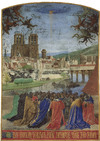
\includegraphics[keepaspectratio,width=\textwidth]{The-Right-Hand-of-God-Protecting-the-Faithful-against-the-Demons-small.jpg}
  \captionart{TheRightHandOfGodAgainstDemons}
  \label{fig:therighthandofgod}
\end{figure}

% Force float here
\clearpage{}
\thispagestyle{titleontop}

%SECT. II. MEMB. I. SUBSECT. II.-_A Digression of the nature of Spirits, bad Angels, or Devils, and how they cause Melancholy_.
\section[Nature of bad Angels, or Devils]{A Digression of the nature of Spirits, bad Angels, or Devils, and how they cause Melancholy.}

\lettrine{H}{ow} far the power of spirits and devils doth extend, and whether they
can cause this, or any other disease, is a serious question, and worthy
to be considered: for the better understanding of which, I will make a
brief digression of the nature of spirits. And although the question be
very obscure, according to Postellus\authormarginnote{1118}, full of controversy and
ambiguity, beyond the reach of human capacity, \lit{I confess I am not able to
understand it}{fateor excedere vires
intentionis meae}, saith \Austin{}\authormarginnote{1119}[2\baselineskip], \li{finitum de infinito non potest statuere}, we can sooner
determine with Tully, \li{de nat. deorum, quid non sint, quam quid sint},
our subtle schoolmen, Cardans, Scaligers, profound Thomists,
Fracastoriana and Ferneliana acies, are weak, dry, obscure, defective
in these mysteries, and all our quickest wits, as an owl's eyes at the
sun's light, wax dull, and are not sufficient to apprehend them; yet,
as in the rest, I will adventure to say something to this point. In
former times, as we read, Acts \rn{xxiii.}, the Sadducees denied that there
were any such spirits, devils, or angels. So did Galen the physician,
the Peripatetics, even \Aristotle himself, as Pomponatius stoutly
maintains, and Scaliger in some sort grants. Though Dandinus the
Jesuit, com. in lib. 2. de anima, stiffly denies it; \li{substantiae
separatae} and intelligences, are the same which Christians call angels,
and Platonists devils, for they name all the spirits, daemones, be they
good or bad angels, as \textlatin{Julius Pollux Onomasticon}, lib. 1. cap. 1.
observes. Epicures and atheists are of the same mind in general,
because they never saw them. Plato, Plotinus, Porphyrius, Jamblichus,
Proclus, insisting in the steps of \textlatin{Trismegistus}, Pythagoras and
Socrates, make no doubt of it: nor Stoics, but that there are such
spirits, though much erring from the truth. Concerning the first
beginning of them, the Talmudists say\authormarginnote{1120} that Adam had a wife called
Lilis, before he married Eve, and of her he begat nothing but devils.
The Turks' Alcoran\authormarginnote{1121}[1\baselineskip] is altogether as absurd and ridiculous in this
point: but the Scripture informs us Christians, how Lucifer, the chief
of them, with his associates, fell\authormarginnote{1122} from heaven for his pride and
ambition; created of God, placed in heaven, and sometimes an angel of
light, now cast down into the lower aerial sublunary parts, or into
hell, and delivered into chains of darkness (2 Pet. \rn{ii.} 4.) to be kept
unto damnation.

\subsection{Nature of Devils.}
There is a foolish opinion which some hold, that
they are the souls of men departed, good and more noble were deified,
the baser grovelled on the ground, or in the lower parts, and were
devils, the which with Tertullian, Porphyrius the philosopher, M.
Tyrius, ser. 27 maintains. These spirits, he saith\authormarginnote{1123}, which we call
angels and devils, are nought but souls of men departed, which either
through love and pity of their friends yet living, help and assist
them, or else persecute their enemies, whom they hated, as Dido
threatened to persecute Aeneas:
\li{Omnibus umbra locis adero: dabis improbe poenas.}

My angry ghost arising from the deep,
Shall haunt thee waking, and disturb thy sleep;
At least my shade thy punishment shall know,
And Fame shall spread the pleasing news below.

They are (as others suppose) appointed by those higher powers to keep
men from their nativity, and to protect or punish them as they see
cause: and are called boni et mali Genii by the Romans. Heroes, lares,
if good, lemures or larvae if bad, by the stoics, governors of
countries, men, cities, saith \Apuleius\authormarginnote{1124}, \li{Deos appellant qui ex
hominum numero juste ac prudenter vitae curriculo gubernato, pro
numine, postea ab hominibus praediti fanis et ceremoniis vulgo
admittuntur, ut in Aegypto Osyris, \etc{}}\authorlatintrans{1124.5}. Praestites, Capella calls them,
which protected particular men as well as princes, Socrates had his
\li{Daemonium Saturninum et ignium}, which of all spirits is best, \li{ad
sublimes cogitationes animum erigentem}, as the Platonists supposed;
Plotinus his, and we Christians our assisting angel, as Andreas
Victorellus, a copious writer of this subject, Lodovicus de La-Cerda,
the Jesuit, in his voluminous tract de Angelo Custode, Zanchius, and
some divines think. But this absurd tenet of Tyreus, Proclus confutes
at large in his book \textlatin{de Anima et daemone}.
Psellus\authorfootnote{1125}, a Christian, and sometimes tutor (saith Cuspinian) to
Michael Parapinatius, Emperor of Greece, a great observer of the nature
of devils, holds\authorfootnote{1126} they are corporeal, and have aerial bodies,
that they are mortal, live and die, (which Martianus Capella likewise
maintains, but our Christian philosophers explode) that they are
nourished and have excrements\authorfootnote{1127}, they feel pain if they be hurt (which
Cardan confirms, and Scaliger justly laughs him to scorn for; \li{Si
pascantur aere, cur non pugnant ob puriorem aera?} \etc{}) or stroken: and
if their bodies be cut, with admirable celerity they come together
again. \Austin{}, in Gen. lib. \rn{iii.} lib. arbit., approves as much, \li{mutata
casu corpora in deteriorem qualitatem aeris spissioris}, so doth
Hierome. Comment. in epist. ad Ephes. cap. 3, Origen, Tertullian,
Lactantius, and many ancient Fathers of the Church: that in their fall
their bodies were changed into a more aerial and gross substance.
Bodine, lib. 4, \textlatin{Theatri Naturae} and David Crusius, \textlatin{Hermeticae
Philosophiae}, lib. 1. cap. 4, by several arguments proves angels and
spirits to be corporeal: \li{quicquid continetur in loco corporeum est; At
spiritus continetur in loco, ergo. Si spiritus sunt quanti}\authorlatintrans{1128}, \li{erunt
corporei: At sunt quanti, ergo. sunt finiti, ergo. quanti, \etc{}.} Bodine
goes\authorfootnote{1129} farther yet, and will have these, \li{Animae separatae genii},
spirits, angels, devils, and so likewise souls of men departed, if
corporeal (which he most eagerly contends) to be of some shape, and
that absolutely round, like Sun and Moon, because that is the most
perfect form, \li{quae nihil habet asperitatis, nihil angulis incisum,
nihil anfractibus involutem, nihil eminens, sed inter corpora perfecta
est perfectissimum}\authorlatintrans{1130}; therefore all spirits are corporeal he
concludes, and in their proper shapes round. That they can assume other
aerial bodies, all manner of shapes at their pleasures, appear in what
likeness they will themselves, that they are most swift in motion, can
pass many miles in an instant, and so likewise transform bodies\authorfootnote{1131}
of others into what shape they please, and with admirable celerity
remove them from place to place; (as the Angel did Habakkuk to Daniel,
and as Philip the deacon was carried away by the Spirit, when he had
baptised the eunuch; so did Pythagoras and Apollonius remove themselves
and others, with many such feats) that they can represent castles in
the air, palaces, armies, spectrums, prodigies, and such strange
objects to mortal men's eyes, cause smells\authorfootnote{1132}, savours, \etc{}, deceive
all the senses; most writers of this subject credibly believe; and that
they can foretell future events, and do many strange miracles. Juno's
image spake to Camillus, and Fortune's statue to the Roman matrons,
with many such. Zanchius, Bodine, Spondanus, and others, are of opinion
that they cause a true metamorphosis, as Nebuchadnezzar was really
translated into a beast, Lot's wife into a pillar of salt; Ulysses'
companions into hogs and dogs, by Circe's charms; turn themselves and
others, as they do witches into cats, dogs, hares, crows, \etc{}. Strozzius
Cicogna hath many examples, lib. \rn{iii.} omnif. mag. cap. 4 and 5, which
he there confutes, as \Austin{} likewise doth, de civ. Dei lib. \rn{xviii.}
That they can be seen when and in what shape, and to whom they will,
saith Psellus, \li{Tametsi nil tale viderim, nec optem videre}, though he
himself never saw them nor desired it; and use sometimes carnal
copulation (as elsewhere I shall prove\authorfootnote{1133} more at large) with women
and men. Many will not believe they can be seen, and if any man shall
say, swear, and stiffly maintain, though he be discreet and wise,
judicious and learned, that he hath seen them, they account him a
timorous fool, a melancholy dizzard, a weak fellow, a dreamer, a sick
or a mad man, they contemn him, laugh him to scorn, and yet Marcus of
his credit told Psellus that he had often seen them. And Leo Suavius, a
Frenchman, c. 8, in Commentar. l. 1. \li{Paracelsi de vita longa}, out of
some Platonists, will have the air to be as full of them as snow
falling in the skies, and that they may be seen, and withal sets down
the means how men may see them; \li{Si irreverberatus oculis sole
splendente versus caelum continuaverint obtutus}\authorlatintrans{1134}, \etc{}, and saith
moreover he tried it, \li{praemissorum feci experimentum}, and it was true,
that the Platonists said. Paracelsus confesseth that he saw them diverse
times, and conferred with them, and so doth Alexander ab
Alexandro\authorfootnote{1135}, that he so found it by experience, when as before he
doubted of it. Many deny it, saith Lavater, \textlatin{de spectris}, part 1. c. 2,
and part 2. c. 11, because they never saw them themselves; but as he
reports at large all over his book, especially c. 19. part 1, they are
often seen and heard, and familiarly converse with men, as Lod. Vives
assureth us, innumerable records, histories, and testimonies evince in
all ages, times, places, and all travellers\authorfootnote{1136} besides; in the West
Indies and our northern climes, \li{Nihil familiarius quam in agris et
urbibus spiritus videre, audire qui vetent, jubeant, \etc{}.} Hieronymus
vita Pauli, Basil ser. 40, Nicephorus, Eusebius, Socrates, Sozomenus,
Jacobus Boissardus\authorfootnote{1137} in his tract de spirituum apparitionibus,
Petrus Loyerus l. \textlatin{de spectris}, Wierus l. 1. have infinite variety of
such examples of apparitions of spirits, for him to read that farther
doubts, to his ample satisfaction. One alone I will briefly insert. A
nobleman in Germany was sent ambassador to the King of Sweden (for his
name, the time, and such circumstances, I refer you to Boissardus, mine
Author\authorfootnote{1138}). After he had done his business, he sailed to Livonia, on
set purpose to see those familiar spirits, which are there said to be
conversant with men, and do their drudgery works. Amongst other
matters, one of them told him where his wife was, in what room, in what
clothes, what doing, and brought him a ring from her, which at his
return, non sine omnium admiratione, he found to be true; and so
believed that ever after, which before he doubted of. Cardan, l. 19. de
subtil, relates of his father, Facius Cardan, that after the accustomed
solemnities, \emph{anno} 1491, 13 August, he conjured up seven devils, in
Greek apparel, about forty years of age, some ruddy of complexion, and
some pale, as he thought; he asked them many questions, and they made
ready answer, that they were aerial devils, that they lived and died as
men did, save that they were far longer lived (700 or 800 years\authorfootnote{1139});
they did as much excel men in dignity as we do juments, and were as far
excelled again of those that were above them; our \authorfootnote{1140}governors and
keepers they are moreover, which Plato in Critias delivered\authorfootnote{1141} of
old, and subordinate to one another, \li{Ut enim homo homini sic daemon
daemoni dominatur}, they rule themselves as well as us, and the spirits
of the meaner sort had commonly such offices, as we make horse-keepers,
neat-herds, and the basest of us, overseers of our cattle; and that we
can no more apprehend their natures and functions, than a horse a
man's. They knew all things, but might not reveal them to men; and
ruled and domineered over us, as we do over our horses; the best kings
amongst us, and the most generous spirits, were not comparable to the
basest of them. Sometimes they did instruct men, and communicate their
skill, reward and cherish, and sometimes, again, terrify and punish, to
keep them in awe, as they thought fit, \li{Nihil magis cupientes} (saith
Lysius, Phis. Stoicorum) \li{quam adorationem hominum}\authorlatintrans{1142}. The same
Author, Cardan, in his Hyperchen, out of the doctrine of Stoics, will
have some of these genii (for so he calls them) to be desirous of
men's company\authorfootnote{1143}, very affable and familiar with them, as dogs are;
others, again, to abhor as serpents, and care not for them. The same
belike Tritemius calls Ignios \li{et sublunares, qui nunquam demergunt ad
inferiora, aut vix ullum habent in terris commercium}: Generally
they far excel men in worth\authorfootnote{1144}, as a man the meanest worm; though some of
them are inferior to those of their own rank in worth, as the
blackguard in a prince's court, and to men again, as some degenerate,
base, rational creatures, are excelled of brute beasts.
That they are mortal, besides these testimonies of Cardan, Martianus,
\etc{}, many other divines and philosophers hold, \li{post prolixum tempus
moriuntur omnes}; The Platonists\authorfootnote{1145}, and some Rabbins, Porphyrius and
Plutarch, as appears by that relation of Thamus: The great God
Pan is dead\authorfootnote{1146}; Apollo Pythius ceased; and so the rest. St. Hierome, in
the life of Paul the Hermit, tells a story how one of them appeared to
St. Anthony in the wilderness, and told him as much. Paracelsus
of our late writers stiffly maintains\authorfootnote{1147} that they are mortal, live and
die as other creatures do. Zozimus, l. 2, farther adds, that religion
and policy dies and alters with them. The Gentiles' gods, he
saith\authorfootnote{1148}, were expelled by Constantine, and together with them. \lit{The fortune
and majesty of the Roman Empire decayed and vanished}{Imperii
Romani majestas, et fortuna interiit, et profligata est}; as that heathen
in Minutius formerly bragged\authorfootnote{1149}, when the Jews were overcome by the
Romans, the Jew's God was likewise captivated by that of Rome; and
Rabsakeh to the Israelites, no God should deliver them out of the hands
of the Assyrians. But these paradoxes of their power, corporeity,
mortality, taking of shapes, transposing bodies, and carnal
copulations, are sufficiently confuted by Zanch. c. 10, l. 4. Pererius
in his comment, and Tostatus questions on the 6th of Gen. Th. Aquin.,
St. \Austin{}, Wierus, Th. Erastus, Delrio, tom. 2, l. 2, quaest. 29;
Sebastian Michaelis, c. 2, de spiritibus, D. Reinolds Lect. 47. They
may deceive the eyes of men, yet not take true bodies, or make a real
metamorphosis; but as Cicogna proves at large, they are
Illusoriae\authorfootnote{1150}, \li{et praestigiatrices transformationes}, omnif. mag.
lib. 4. cap. 4, mere illusions and cozenings, like that tale of Pasetis
obulus in Suidas, or that of Autolicus, Mercury's son, that dwelt in
Parnassus, who got so much treasure by cozenage and stealth. His father
Mercury, because he could leave him no wealth, taught him many fine
tricks to get means, for he could drive away men's cattle\authorfootnote{1151}, and if
any pursued him, turn them into what shapes he would, and so did
mightily enrich himself, \li{hoc astu maximam praedam est adsecutus}. This,
no doubt, is as true as the rest; yet thus much in general. Thomas,
Durand, and others, grant that they have understanding far beyond men,
can probably conjecture and foretell\authorfootnote{1152} many things; they can cause
and cure most diseases, deceive our senses; they have excellent skill
in all Arts and Sciences; and that the most illiterate devil is \lit{more knowing than any man}{Quovis
homine scientior}, as Cicogna maintains\authorfootnote{1153} out of others. They know the virtues of herbs, plants, stones, minerals, \etc{}; of all creatures, birds, beasts, the four
elements, stars, planets, can aptly apply and make use of them as they
see good; perceiving the causes of all meteors, and the like: \li{Dant se
coloribus} (as \Austin{} hath\authorfootnote{1154} it) \li{accommodant se figuris, adhaerent
sonis, subjiciunt se odoribus, infundunt se saporibus, omnes sensus
etiam ipsam intelligentiam daemones fallunt}, they deceive all our
senses, even our understanding itself at once. They can produce\authorfootnote{1155}
miraculous alterations in the air, and most wonderful effects, conquer
armies, give victories, help, further, hurt, cross and alter human
attempts and projects (\li{Dei permissu}) as they see good themselves.
When Charles the Great intended\authorfootnote{1156} to make a channel betwixt the
Rhine and the Danube, look what his workmen did in the day, these
spirits flung down in the night, \li{Ut conatu Rex desisteret, pervicere}.
Such feats can they do. But that which Bodine, l. 4, Theat. nat. thinks
(following Tyrius belike, and the Platonists), they can tell the
secrets of a man's heart, \li{aut cogitationes hominum}, is most false; his
reasons are weak, and sufficiently confuted by Zanch. lib. 4, cap. 9.
Hierom. lib. 2, com. in Mat. ad cap. 15, Athanasius quaest. 27, ad
Antiochum Principem, and others.

\subsection{Orders.}
As for those orders of good and bad devils, which the
Platonists hold, is altogether erroneous, and those Ethnics \li{boni et
mali Genii}, are to be exploded: these heathen writers agree not in this
point among themselves, as Dandinus notes, \li{An sint mali non
conveniunt}\authorfootnote{1157}, some will have all spirits good or bad to us by a mistake,
as if an Ox or Horse could discourse, he would say the Butcher was his
enemy because he killed him, the grazier his friend because he fed him;
a hunter preserves and yet kills his game, and is hated nevertheless of
his game; nec piscatorem piscis amare potest, \etc{}. But Jamblichus,
Psellus, Plutarch, and most Platonists acknowledge bad, et ab eorum
maleficiis cavendum, and we should beware of their wickedness, for they
are enemies of mankind, and this Plato learned in Egypt, that they
quarrelled with Jupiter, and were driven by him down to hell.
That\authorfootnote{1158} which \Apuleius\authorfootnote{1159}, Xenophon, and Plato contend of
Socrates Daemonium, is most absurd: That which Plotinus of his, that he
had likewise Deum pro Daemonio; and that which Porphyry concludes of
them all in general, if they be neglected in their sacrifice they are
angry; nay more, as Cardan in his Hipperchen will, they feed on men's
souls, \li{Elementa sunt plantis elementum, animalibus plantae, hominibus
animalia, erunt et homines aliis, non autem diis, nimis enim remota est
eorum natura a nostra, quapropter daemonibus}: and so belike that we
have so many battles fought in all ages, countries, is to make them a
feast, and their sole delight: but to return to that I said before, if
displeased they fret and chafe, (for they feed belike on the souls of
beasts, as we do on their bodies) and send many plagues amongst us; but
if pleased, then they do much good; is as vain as the rest and confuted
by \Austin{}, l. 9. c. 8. de Civ. Dei. Euseb. l. 4. praepar. Evang. c. 6.
and others. Yet thus much I find, that our schoolmen and other
divines make nine kinds of bad spirits\authorfootnote{1160}, as Dionysius hath done of
angels. In the first rank are those false gods of the gentiles, which
were adored heretofore in several idols, and gave oracles at Delphos,
and elsewhere; whose prince is Beelzebub. The second rank is of liars
and equivocators, as Apollo, Pythius, and the like. The third are those
vessels of anger, inventors of all mischief; as that Theutus in Plato;
Esay calls them vessels of fury\authorfootnote{1161}; their prince is Belial. The
fourth are malicious revenging devils; and their prince is Asmodaeus.
The fifth kind are cozeners, such as belong to magicians and witches;
their prince is Satan. The sixth are those aerial devils that
corrupt the air\authorfootnote{1162} and cause plagues, thunders, fires, \etc{}; spoken
of in the Apocalypse, and Paul to the Ephesians names them the princes
of the air; Meresin is their prince. The seventh is a destroyer,
captain of the furies, causing wars, tumults, combustions, uproars,
mentioned in the Apocalypse; and called Abaddon. The eighth is that
accusing or calumniating devil, whom the Greeks call \textgreek{Διαβολος}, that
drives men to despair. The ninth are those tempters in several kinds,
and their prince is Mammon. Psellus makes six kinds, yet none above the
Moon: Wierus in his Pseudo-monarchia Daemonis, out of an old book,
makes many more divisions and subordinations, with their several names,
numbers, offices, \etc{}, but Gazaeus cited by Lipsius\authorfootnote{1163} will have all
places full of angels, spirits, and devils, above and beneath the
Moon, ethereal and aerial\authorfootnote{1164}, which \Austin{} cites out of Varro l. 7.
de Civ. Dei, c. 6. The celestial devils above, and aerial beneath, or,
as some will, gods above, Semi-dei or half gods beneath, Lares, Heroes,
Genii, which climb higher, if they lived well, as the Stoics held; but
grovel on the ground as they were baser in their lives, nearer to the
earth: and are Manes, Lemures, Lamiae, \etc{}. They will have no
place\authorfootnote{1165} but all full of spirits, devils, or some other inhabitants;
\li{Plenum Caelum, aer, aqua terra, et omnia sub terra}, saith
Gazaeus\authorfootnote{1166}; though Anthony Rusca in his book de Inferno, lib. \rn{v.}
cap. 7. would confine them to the middle region, yet they will have
them everywhere. Not so much as a hair-breadth empty in heaven, earth,
or waters, above or under the earth. The air is not so full of flies in
summer, as it is at all times of invisible devils: this
Paracelsus stiffly maintains\authorfootnote{1167}, and that they have every one their
several chaos, others will have infinite worlds, and each world his
peculiar spirits, gods, angels, and devils to govern and punish it.
\li{Singula nonnulli credunt quoque sidera posse
Dici orbes, terramque appellant sidus opacum,
Cui minimus divum praesit.}\authorfootnote{1168}---

Some persons believe each star to be a world, and this earth an opaque
star, over which the least of the gods presides.

Gregorius Tholsanus makes\authorfootnote{1169} seven kinds of ethereal spirits or
angels, according to the number of the seven planets, Saturnine,
Jovial, Martial, of which Cardan discourseth lib. 20. de subtil. he
calls them substantias primas, Olympicos daemones Tritemius, qui
praesunt Zodiaco, \etc{}, and will have them to be good angels above,
devils beneath the Moon, their several names and offices he there sets
down, and which Dionysius of Angels, will have several spirits for
several countries, men, offices, \etc{}, which live about them, and as so
many assisting powers cause their operations, will have in a word,
innumerable, as many of them as there be stars in the skies.
Marcilius Ficinus seems to second\authorfootnote{1170} this opinion, out of Plato, or
from himself, I know not, (still ruling their inferiors, as they do
those under them again, all subordinate, and the nearest to the earth
rule us, whom we subdivide into good and bad angels, call gods or
devils, as they help or hurt us, and so adore, love or hate) but it is
most likely from Plato, for he relying wholly on Socrates, \li{quem mori
potius quam mentiri voluisse scribit}, whom he says would rather die
than tell a falsehood, out of Socrates' authority alone, made nine
kinds of them: which opinion belike Socrates took from Pythagoras, and
he from \textlatin{Trismegistus}, he from Zoroastes, first God, second idea, 3.
Intelligences, 4. Arch-Angels, 5. Angels, 6. Devils, 7. Heroes, 8.
Principalities, 9. Princes: of which some were absolutely good, as
gods, some bad, some indifferent \li{inter deos et homines}, as heroes and
daemons, which ruled men, and were called \li{genii}, or as Proclus\authorfootnote{1171}
and Jamblichus will, the middle betwixt God and men. Principalities and
princes, which commanded and swayed kings and countries; and had
several places in the spheres perhaps, for as every sphere is higher,
so hath it more excellent inhabitants: which belike is that Galilaeus a
Galileo and Kepler aims at in his \textlatin{nuncio Syderio}, when he will have
Saturnine\authorfootnote{1172} and Jovial inhabitants: and which Tycho Brahe doth in
some sort touch or insinuate in one of his epistles: but these things
Zanchius justly explodes\authorfootnote{1173}, cap. 3. lib. 4. P. Martyr, in 4. Sam. 28.

So that according to these men the number of ethereal spirits must
needs be infinite: for if that be true that some of our mathematicians
say: if a stone could fall from the starry heaven, or eighth sphere,
and should pass every hour an hundred miles, it would be 65 years, or
more, before it would come to ground, by reason of the great distance
of heaven from earth, which contains as some say 170 millions 800
miles, besides those other heavens, whether they be crystalline or
watery which Maginus adds, which peradventure holds as much more, how
many such spirits may it contain? And yet for all this Thomas
Albertus\authorfootnote{1174}, and most hold that there be far more angels than devils.

\subsection{Sublunary devils, and their kinds.}
But be they more or less, \lit{what is beyond our comprehension does not
concern us}{Quod supra nos nihil ad nos}. Howsoever as Martianus foolishly supposeth, \li{Aetherii
Daemones non curant res humanas}, they care not for us, do not attend
our actions, or look for us, those ethereal spirits have other worlds
to reign in belike or business to follow. We are only now to speak in
brief of these sublunary spirits or devils: for the rest, our divines
determine that the devil had no power over stars, or heavens;
\lit{by their charms (verses) they can seduce the moon from the heavens}{Carminibus coelo possunt deducere lunam}\authorfootnote{1175}, \etc{}. Those are poetical
fictions, and that they can \lit{stop rivers and turn the stars backward in their courses}{sistere aquam fluviis, et vertere
sidera retro}\authorfootnote{1176}, \etc{}, as Canadia in \Horace{}, 'tis all false. They are confined
until the day of judgment to this sublunary world\authorfootnote{1177}, and can work no
farther than the four elements, and as God permits them. Wherefore of
these sublunary devils, though others divide them otherwise according
to their several places and offices, Psellus makes six kinds, fiery,
aerial, terrestrial, watery, and subterranean devils, besides those
fairies, satyrs, nymphs, \etc{}.

Fiery spirits or devils are such as commonly work by blazing stars,
fire-drakes, or \li{ignes fatui}; which lead men often in \li{flumina aut
praecipitia}, saith Bodine, lib. 2. Theat. Naturae, fol. 221. \lit{whom if travellers wish to keep off they must pronounce the name of God with a clear voice, or adore him with their faces in contact with the ground, \etc{}}{Quos inquit arcere si volunt viatores, clara voce Deum appellare aut pronam
facie terram contingente adorare oportet, et hoc amuletum majoribus
nostris acceptum ferre debemus}, \etc{}; likewise they
counterfeit suns and moons, stars oftentimes, and sit on ship masts: \li{In
navigiorum summitatibus visuntur}; and are called \li{dioscuri}, as Eusebius
l. contra Philosophos, c. \rn{xlviii.} informeth us, out of the authority of
Zenophanes; or little clouds, \li{ad motum nescio quem volantes}; which
never appear, saith Cardan, but they signify some mischief or other to
come unto men, though some again will have them to pretend good, and
victory to that side they come towards in sea fights, St. Elmo's fires
they commonly call them, and they do likely appear after a sea storm;
Radzivilius, the Polonian duke, calls this apparition, Sancti Germani
sidus; and saith moreover that he saw the same after in a storm, as he
was sailing, 1582, from Alexandria to Rhodes. Our stories are
full\authorfootnote{1178} of such apparitions in all kinds. Some think they keep their
residence in that Hecla, a mountain in Iceland, Aetna in Sicily,
Lipari, Vesuvius, \etc{}. These devils were worshipped heretofore by that
superstitious Pyromanteia\authormarginnote{1179} and the like.

Aerial spirits or devils, are such as keep quarter most part in the
air\authorfootnote{1180}, cause many tempests, thunder, and lightnings, tear oaks,
fire steeples, houses, strike men and beasts, make it rain stones, as
in Livy's time, wool, frogs, \etc{}. Counterfeit armies in the air, strange
noises, swords, \etc{}, as at Vienna before the coming of the Turks, and
many times in Rome, as Scheretzius l. de spect. c. 1. part 1. Lavater
de spect. part. 1. c. 17. Julius Obsequens, an old Roman, in his book
of prodigies, \emph{ab urb. cond.} 505. Machiavel hath illustrated\authorfootnote{1181} by
many examples, and Josephus, in his book de bello Judaico, before the
destruction of Jerusalem. All which Guil. Postellus, in his first book,
c. 7, \textlatin{de orbis concordia}, useth as an effectual argument (as indeed it
is) to persuade them that will not believe there be spirits or devils.
They cause whirlwinds on a sudden, and tempestuous storms; which though
our meteorologists generally refer to natural causes, yet I am of
Bodine's mind, Theat. Nat. l. 2. they are more often caused by those
aerial devils, in their several quarters; for Tempestatibus se
ingerunt, saith \authorfootnote{1182} Rich. Argentine; as when a desperate man makes
away with himself, which by hanging or drowning they frequently do, as
Kommanus observes, \textlatin{de mirac. mort. part. 7, c. 76. tripudium agentes},
dancing and rejoicing at the death of a sinner. These can corrupt the
air, and cause plagues, sickness, storms, shipwrecks, fires,
inundations. At Mons Draconis in Italy, there is a most memorable
example in Jovianus Pontanus\authorfootnote{1183}: and nothing so familiar (if we may
believe those relations of \textlatin{Saxo Grammaticus, Olaus Magnus, Damianus} A.
Goes) as for witches and sorcerers, in Lapland, Lithuania, and all over
Scandia, to sell winds to mariners, and cause tempests, which Marcus
Paulus the Venetian relates likewise of the Tartars. These kind of
devils are much delighted in sacrifices\authorfootnote{1184} (saith Porphyry), held
all the world in awe, and had several names, idols, sacrifices, in
Rome, Greece, Egypt, and at this day tyrannise over, and deceive those
Ethnics and Indians, being adored and worshipped for gods\authorfootnote{1185}. For
the Gentiles' gods were devils (as \textlatin{Trismegistus} confesseth\authorfootnote{1186} in his
Asclepius), and he himself could make them come to their images by
magic spells: and are now as much respected by our papists (saith
Pictorius\authorfootnote{1187}) under the name of saints. These are they which Cardan
thinks desire so much carnal copulation with witches (Incubi and
Succubi), transform bodies, and are so very cold, if they be touched;
and that serve magicians. His father had one of them (as he is not
ashamed to relate), an aerial devil\authorfootnote{1188}, bound to him for twenty and
eight years. As Agrippa's dog had a devil tied to his collar; some
think that Paracelsus (or else Erastus belies him) had one confined to
his sword pummel; others wear them in rings, \etc{}. Jannes and Jambres did
many things of old by their help; Simon Magus, Cinops, Apollonius
Tianeus, Jamblichus, and Tritemius of late, that showed Maximilian the
emperor his wife, after she was dead; Et verrucam in collo ejus (saith
Godolman\authorfootnote{1189}) so much as the wart in her neck. Delrio, lib. 2. hath
diverse examples of their feats: Cicogna, lib. 3. cap. 3. and Wierus in
his book \textlatin{de praestig. daemonum. Boissardus de magis et veneficis}.
Water-devils are those Naiads or water nymphs which have been
heretofore conversant about waters and rivers. The water (as Paracelsus
thinks) is their chaos, wherein they live; some call them fairies, and
say that Habundia is their queen; these cause inundations, many times
shipwrecks, and deceive men diverse ways, as Succuba, or otherwise,
appearing most part (saith Tritemius) in women's shapes.

Paracelsus hath several stories\authorfootnote{1190} of them that have lived and been
married to mortal men, and so continued for certain years with them,
and after, upon some dislike, have forsaken them. Such a one as
Aegeria, with whom Numa was so familiar, Diana, Ceres, \etc{}. Olaus
Magnus hath\authorfootnote{1191} a long narration of one Hotherus, a king of Sweden, that
having lost his company, as he was hunting one day, met with these
water nymphs or fairies, and was feasted by them; and Hector Boethius,
or Macbeth, and Banquo, two Scottish lords, that as they were wandering
in the woods, had their fortunes told them by three strange women. To
these, heretofore, they did use to sacrifice, by that \textgreek{ὑδρομαντέια}, or
divination by waters.

Terrestrial devils are those Lares\authorfootnote{1192}, genii, fauns, satyrs, 
wood-nymphs\authorfootnote{1193}, foliots, fairies, Robin Goodfellows, trulli, \etc{}, which as
they are most conversant with men, so they do them most harm. Some
think it was they alone that kept the heathen people in awe of old, and
had so many idols and temples erected to them. Of this range was Dagon
amongst the Philistines, Bel amongst the Babylonians, Astartes amongst
the Sidonians, Baal amongst the Samaritans, Isis and Osiris amongst the
Egyptians, \etc{}; some put our fairies\authorfootnote{1194} into this rank, which have
been in former times adored with much superstition, with sweeping their
houses, and setting of a pail of clean water, good victuals, and the
like, and then they should not be pinched, but find money in their
shoes, and be fortunate in their enterprises. These are they that dance
on heaths and greens, as Lavater thinks\authorfootnote{1195} with Tritemius, and as
Olaus Magnus adds\authorfootnote{1196}, leave that green circle, which we commonly
find in plain fields, which others hold to proceed from a meteor
falling, or some accidental rankness of the ground, so nature sports
herself; they are sometimes seen by old women and children. Hierom.
Pauli, in his description of the city of Bercino in Spain, relates how
they have been familiarly seen near that town, about fountains and
hills; \li{Nonnunquam} (saith Tritemius) \li{in sua latibula montium
simpliciores homines ducant, stupenda mirantibus ostentes miracula,
nolarum sonitus, spectacula}\authorlatintrans{1197}. Giraldus Cambrensis gives
instance in a monk of Wales that was so deluded. Paracelsus
reckons\authorfootnote{1198} up many places in Germany, where they do usually walk in little
coats, some two feet long. A bigger kind there is of them called with
us hobgoblins, and Robin Goodfellows, that would in those superstitious
times grind corn for a mess of milk, cut wood, or do any manner of
drudgery work. They would mend old irons in those Aeolian isles of
Lipari, in former ages, and have been often seen and heard.
Tholosanus calls\authorfootnote{1199} them trullos and Getulos, and saith, that in his
days they were common in many places of France. Dithmarus Bleskenius,
in his description of Iceland, reports for a certainty, that almost in
every family they have yet some such familiar spirits; and Felix
Malleolus, in his book de crudel. daemon. affirms as much, that these
trolli or telchines are very common in Norway, and seen\authorfootnote{1200} to do
drudgery work; to draw water, saith Wierus, lib. 1. cap. 22, dress
meat, or any such thing. Another sort of these there are, which
frequent forlorn houses\authormarginnote{1201}, which the Italians call foliots, most
part innoxious, Cardan holds\authorfootnote{1202}; They will make strange noises in
the night, howl sometimes pitifully, and then laugh again, cause great
flame and sudden lights, fling stones, rattle chains, shave men, open
doors and shut them, fling down platters, stools, chests, sometimes
appear in the likeness of hares, crows, black dogs, \etc{} of which read
Pet Thyraeus the Jesuit\authorfootnote{1203}, in his \textlatin{Tract, de locis infestis, part.
1. et cap. 4}, who will have them to be devils or the souls of damned
men that seek revenge, or else souls out of purgatory that seek ease;
for such examples peruse Sigismundus Scheretzius\authorfootnote{1204}, \textlatin{lib. de
spectris, part 1. c. 1.} which he saith he took out of Luther most part;
there be many instances. Plinius Secundus remembers\authorfootnote{1205} such a house
at Athens, which Athenodorus the philosopher hired, which no man durst
inhabit for fear of devils. \Austin{}, \textlatin{de Civ. Dei. lib. 22, cap. 1.}
relates as much of Hesperius the Tribune's house, at Zubeda, near their
city of Hippos, vexed with evil spirits, to his great hindrance, \li{Cum
afflictione animalium et servorum suorum.} Many such instances are to be
read in Niderius Formicar, lib. 5. cap. \rn{xii.} 3. \etc{}. Whether I may call
these Zim and Ochim, which Isaiah, cap. \rn{xiii.} 21. speaks of, I make a
doubt. See more of these in the said Scheretz. lib. 1. de spect. cap.
4. he is full of examples. These kind of devils many times appear to
men, and affright them out of their wits, sometimes walking at
noonday\authorfootnote{1206}, sometimes at nights, counterfeiting dead men's ghosts,
as that of Caligula, which (saith Suetonius) was seen to walk in
Lavinia's garden, where his body was buried, spirits haunted, and the
house where he died, \li{Nulla nox sine terrore transacta, donec
incendio consumpta}\authorfootnote{1207}; every night this happened, there was no quietness,
till the house was burned. About Hecla, in Iceland, ghosts commonly
walk, \li{animas mortuorum simulantes}, saith Joh. Anan, lib. 3. de nat.
daem. Olaus. lib. 2. cap. 2. Natal Tallopid. lib. de apparit. spir.
Kornmannus de mirac. mort. part. 1. cap. 44. such sights are frequently
seen circa sepulchra et monasteria, saith Lavat. lib. 1. cap. 19. in
monasteries and about churchyards, \lit{marshes, great buildings,
solitary places, or remarkable as the scene of some murder}{loca paludinosa, ampla aedificia,
solitaria, et caede hominum notata}, \etc{}. Thyreus
adds, \lit{where some very heinous crime was
committed, there the impious and infamous generally dwell}{ubi gravius peccatum est commissum, impii, pauperum oppressores
et nequiter insignes habitant}. These
spirits often foretell men's deaths by several signs, as knocking,
groanings, \etc{} though Rich. Argentine\authorfootnote{1208}, c. 18. \textlatin{de praestigiis
daemonum}, will ascribe these predictions to good angels, out of the
authority of Ficinus and others; \lit{prodigies frequently occur at the deaths of
illustrious men}{prodigia in obitu principum saepius
contingunt}, \etc{}, as in the Lateran church in Rome\authorfootnote{1209}, the popes'
deaths are foretold by Sylvester's tomb. Near Rupes Nova in Finland, in
the kingdom of Sweden, there is a lake, in which, before the governor
of the castle dies, a spectrum, in the habit of Arion with his harp,
appears, and makes excellent music, like those blocks in Cheshire,
which (they say) presage death to the master of the family; or that
oak\authorfootnote{1210} in Lanthadran park in Cornwall, which foreshows as much. Many
families in Europe are so put in mind of their last by such
predictions, and many men are forewarned (if we may believe Paracelsus)
by familiar spirits in diverse shapes, as cocks, crows, owls, which
often hover about sick men's chambers, vel quia morientium foeditatem
sentiunt, as Baracellus conjectures\authorfootnote{1211}, \li{et ideo super tectum
infirmorum crocitant}, because they smell a corse; or for that (as
\authorfootnote{1212}Bernardinus de Bustis thinketh) God permits the devil to appear
in the form of crows, and such like creatures, to scare such as live
wickedly here on earth. A little before Tully's death (saith Plutarch)
the crows made a mighty noise about him, tumultuose perstrepentes, they
pulled the pillow from under his head. Rob. Gaguinus, hist. Franc. lib.
8, telleth such another wonderful story at the death of Johannes de
Monteforti, a French lord, \emph{anno} 1345, \lit{a
multitude of crows alighted on the house of the dying man, such as no
one imagined existed in France}{tanta corvorum multitudo
aedibus morientis insedit, quantam esse in Gallia nemo judicasset}. Such prodigies are very frequent in
authors. See more of these in the said Lavater, \textlatin{Thyreus de locis
infestis, part 3, cap. 58. Pictorius, Delrio, Cicogna, lib. 3, cap. 9.}
Necromancers take upon them to raise and lay them at their pleasures:
and so likewise, those which Mizaldus calls ambulones, that walk about
midnight on great heaths and desert places, which (saith \authorfootnote{1213}Lavater)
draw men out of the way, and lead them all night a byway, or quite bar
them of their way; these have several names in several places; we
commonly call them Pucks. In the deserts of Lop, in Asia, such
illusions of walking spirits are often perceived, as you may read in M.
Paulus the Venetian his travels; if one lose his company by chance,
these devils will call him by his name, and counterfeit voices of his
companions to seduce him. Hieronym. Pauli, in his book of the hills of
Spain, relates of a great \authorfootnote{1214}mount in Cantabria, where such
spectrums are to be seen; Lavater and Cicogna have variety of examples
of spirits and walking devils in this kind. Sometimes they sit by the
highway side, to give men falls, and make their horses stumble and
start as they ride (if you will believe the relation of that holy man
Ketellus in \authorfootnote{1215}Nubrigensis), that had an especial grace to see
devils, Gratiam divinitus collatam, and talk with them, Et impavidus
cum spiritibus sermonem miscere, without offence, and if a man curse or
spur his horse for stumbling, they do heartily rejoice at it; with many
such pretty feats.

Subterranean devils are as common as the rest, and do as much harm.
Olaus Magnus, lib. 6, cap. 19, make six kinds of them; some bigger,
some less. These (saith \authorfootnote{1216}Munster) are commonly seen about mines of
metals, and are some of them noxious; some again do no harm. The
metal-men in many places account it good luck, a sign of treasure and
rich ore when they see them. Georgius Agricola, in his book de
subterraneis animantibus, cap. 37, reckons two more notable kinds of
them, which he calls \authorfootnote{1217}getuli and cobali, both are clothed after
the manner of metal-men, and will many times imitate their works. Their
office, as Pictorius and Paracelsus think, is to keep treasure in the
earth, that it be not all at once revealed; and besides, \authorfootnote{1218}Cicogna
avers that they are the frequent causes of those horrible earthquakes
which often swallow up, not only houses, but whole islands and cities;
in his third book, cap. 11, he gives many instances.

The last are conversant about the centre of the earth to torture the
souls of damned men to the day of judgment; their egress and regress
some suppose to be about Etna, Lipari, Mons Hecla in Iceland, Vesuvius,
Terra del Fuego, \etc{}, because many shrieks and fearful cries are
continually heard thereabouts, and familiar apparitions of dead men,
ghosts and goblins.

\subsection{Their Offices, Operations, Study.}
Thus the devil reigns, and in a thousand several shapes, as a roaring lion still seeks whom he may
devour, 1 Pet. \rn{v.}, by sea, land, air, as yet unconfined, though \authorfootnote{1219}
some will have his proper place the air; all that space between us and
the moon for them that transgressed least, and hell for the wickedest
of them, Hic velut in carcere ad finem mundi, tunc in locum funestiorum
trudendi, as \Austin{} holds de Civit. Dei, c. 22, lib. 14, cap. 3 et 23;
but be where he will, he rageth while he may to comfort himself, as
\authorfootnote{1220} Lactantius thinks, with other men's falls, he labours all he can
to bring them into the same pit of perdition with him. For \authorfootnote{1221}men's
miseries, calamities, and ruins are the devil's banqueting dishes. By
many temptations and several engines, he seeks to captivate our souls.
The Lord of Lies, saith \authorfootnote{1222}\Austin{}, as he was deceived himself, he
seeks to deceive others, the ringleader to all naughtiness, as he did
by Eve and Cain, Sodom and Gomorrah, so would he do by all the world.
Sometimes he tempts by covetousness, drunkenness, pleasure, pride, \etc{},
errs, dejects, saves, kills, protects, and rides some men, as they do
their horses. He studies our overthrow, and generally seeks our
destruction; and although he pretend many times human good, and
vindicate himself for a god by curing of several diseases, aegris
sanitatem, et caecis luminis usum restituendo, as \Austin{} declares, lib.
10, de civit Dei, cap. 6, as Apollo, Aesculapius, Isis, of old have
done; divert plagues, assist them in wars, pretend their happiness, yet
nihil his impurius, scelestius, nihil humano generi infestius, nothing
so impure, nothing so pernicious, as may well appear by their
tyrannical and bloody sacrifices of men to Saturn and Moloch, which are
still in use among those barbarous Indians, their several deceits and
cozenings to keep men in obedience, their false oracles, sacrifices,
their superstitious impositions of fasts, penury, \etc{}. Heresies,
superstitious observations of meats, times, \etc{}, by which they \authorfootnote{1223}
crucify the souls of mortal men, as shall be showed in \hyperref[ch:religious-melancholy]{our Treatise of
Religious Melancholy}. \li{Modico adhuc tempore sinitur malignari}, as Bernard expresseth it\authorfootnote{1224}, by God's permission he rageth a while, hereafter
to be confined to hell and darkness, which is prepared for him and his
angels, Mat. \rn{xxv.}

How far their power doth extend it is hard to determine; what the
ancients held of their effects, force and operations, I will briefly
show you: Plato in Critias, and after him his followers, gave out that
these spirits or devils, were men's governors and keepers, our lords
and masters, as we are of our cattle. \authorfootnote{1225}They govern provinces and
kingdoms by oracles, auguries, dreams, rewards and punishments,
prophecies, inspirations, sacrifices, and religious superstitions,
varied in as many forms as there be diversity of spirits; they send
wars, plagues, peace, sickness, health, dearth, plenty, \authorfootnote{1226}Adstantes
hic jam nobis, spectantes, et arbitrantes, \etc{} as appears by those
histories of Thucydides, Livius, Dionysius Halicarnassus, with many
others that are full of their wonderful stratagems, and were therefore
by those Roman and Greek commonwealths adored and worshipped for gods
with prayers and sacrifices, \etc{}. \authorfootnote{1227}In a word, \li{Nihil magis quaerunt
quam metum et admirationem hominum}\authorlatintrans{1228}; and as another hath it, \li{Dici
non potest, quam impotenti ardore in homines dominium, et Divinos
cultus maligni spiritus affectent}\authorlatintrans{1229}. Tritemius in his book de
septem secundis, assigns names to such angels as are governors of
particular provinces, by what authority I know not, and gives them
several jurisdictions. Asclepiades a Grecian, Rabbi Achiba the Jew,
Abraham Avenezra, and Rabbi Azariel, Arabians, (as I find them cited by
\authorfootnote{1230}Cicogna) farther add, that they are not our governors only, Sed
ex eorum concordia et discordia, boni et mali affectus promanant, but
as they agree, so do we and our princes, or disagree; stand or fall.
Juno was a bitter enemy to Troy, Apollo a good friend, Jupiter
indifferent, Aequa Venus Teucris, Pallas iniqua fuit; some are for us
still, some against us, Premente Deo, fert Deus alter opem. Religion,
policy, public and private quarrels, wars are procured by them, and
they are \authorfootnote{1231}delighted perhaps to see men fight, as men are with
cocks, bulls and dogs, bears, \etc{}, plagues, dearths depend on them, our
bene and male esse, and almost all our other peculiar actions (for as
Anthony Rusea contends, lib. 5, cap. 18, every man hath a good and a
bad angel attending on him in particular, all his life long, which
Jamblichus calls \li{daemonem}), preferments, losses, weddings, deaths,
rewards and punishments, and as Proclus will\authorfootnote{1232}, all offices
whatsoever, \li{alii genetricem, alii opificem potestatem habent}, \etc{} and
several names they give them according to their offices, as Lares,
Indegites, Praestites, \etc{}. When the Arcades in that battle at Cheronae,
which was fought against King Philip for the liberty of Greece, had
deceitfully carried themselves, long after, in the very same place,
\li{Diis Graeciae, ultoribus} (saith mine author) they were miserably slain
by Metellus the Roman: so likewise, in smaller matters, they will have
things fall out, as these boni and mali genii favour or dislike us:
Saturni non conveniunt Jovialibus, \etc{}. He that is Saturninus shall
never likely be preferred. \authorfootnote{1233}That base fellows are often advanced,
undeserving Gnathoes, and vicious parasites, whereas discreet, wise,
virtuous and worthy men are neglected and unrewarded; they refer to
those domineering spirits, or subordinate Genii; as they are inclined,
or favour men, so they thrive, are ruled and overcome; for as
\authorfootnote{1234}Libanius supposeth in our ordinary conflicts and contentions,
\lit{one genius yields and is overcome by another}{Genius Genio cedit et obtemperat}. All
particular events almost they refer to these private spirits; and (as
Paracelsus adds) they direct, teach, inspire, and
instruct men. Never was any man extraordinary famous in any art,
action, or great commander, that had not familiarem daemonem to inform
him, as Numa, Socrates, and many such, as Cardan illustrates, cap. 128,
\textlatin{Arcanis prudentiae civilis}, \authorfootnote{1235} \li{Speciali siquidem gratia, se a Deo
donari asserunt magi, a Geniis caelestibus instrui, ab iis doceri}. But
these are most erroneous paradoxes, \li{ineptae et fabulosae nugae},
rejected by our divines and Christian churches. 'Tis true they have, by
God's permission, power over us, and we find by experience, that they
can \authorfootnote{1236}hurt not our fields only, cattle, goods, but our bodies and
minds. At Hammel in Saxony, \emph{anno} 1484. 20 \emph{Junii}, the devil, in
likeness of a pied piper, carried away 130 children that were never
after seen. Many times men are \authorfootnote{1237}affrighted out of their wits,
carried away quite, as Scheretzius illustrates, lib. 1, c. \rn{iv.}, and
severally molested by his means, Plotinus the Platonist, lib. 14,
advers. Gnos. laughs them to scorn, that hold the devil or spirits can
cause any such diseases. Many think he can work upon the body, but not
upon the mind. But experience pronounceth otherwise, that he can work
both upon body and mind. Tertullian is of this opinion, c. 22.
\authorfootnote{1238}That he can cause both sickness and health, and that secretly.
\authorfootnote{1239}Taurellus adds by clancular poisons he can infect the bodies, and
hinder the operations of the bowels, though we perceive it not, closely
creeping into them, saith \authorfootnote{1240}Lipsius, and so crucify our souls: Et
nociva melancholia furiosos efficit. For being a spiritual body, he
struggles with our spirits, saith Rogers, and suggests (according to
\authorfootnote{1241}Cardan, \li{verba sine voce, species sine visu}, envy, lust, anger,
\etc{}) as he sees men inclined.

The manner how he performs it, Biarmannus in his Oration against
Bodine, sufficiently declares. \authorfootnote{1242}He begins first with the phantasy,
and moves that so strongly, that no reason is able to resist. Now the
phantasy he moves by mediation of humours; although many physicians are
of opinion, that the devil can alter the mind, and produce this disease
of himself. Quibusdam medicorum visum, saith \authorfootnote{1243}\Avicenna{}, quod
Melancholia contingat a daemonio. Of the same mind is Psellus and
Rhasis the Arab. lib. 1. Tract. 9. Cont. \authorfootnote{1244}That this disease
proceeds especially from the devil, and from him alone. Arculanus, cap.
6. in 9. Rhasis, Aelianus Montaltus, in his 9. cap. Daniel Sennertus,
lib. 1. part. 2. cap. 11. confirm as much, that the devil can cause
this disease; by reason many times that the parties affected prophesy,
speak strange language, but non sine interventu humoris, not without
the humour, as he interprets himself; no more doth \Avicenna{}, si
contingat a daemonio, sufficit nobis ut convertat complexionem ad
choleram nigram, et sit causa ejus propinqua cholera nigra; the
immediate cause is choler adust, which \authorfootnote{1245} Pomponatius likewise
labours to make good: Galgerandus of Mantua, a famous physician, so
cured a demoniacal woman in his time, that spake all languages, by
purging black choler, and thereupon belike this humour of melancholy is
called balneum diaboli, the devil's bath; the devil spying his
opportunity of such humours drives them many times to despair, fury,
rage, \etc{}, mingling himself among these humours. This is that which
Tertullian avers, Corporibus infligunt acerbos casus, animaeque
repentinos, membra distorquent, occulte repentes, \etc{} and which Lemnius
goes about to prove, Immiscent se mali Genii pravis humoribus, atque
atrae, bili, \etc{}. And \authorfootnote{1246}Jason Pratensis, that the devil, being a
slender incomprehensible spirit, can easily insinuate and wind himself
into human bodies, and cunningly couched in our bowels vitiate our
healths, terrify our souls with fearful dreams, and shake our minds
with furies. And in another place, These unclean spirits settled in our
bodies, and now mixed with our melancholy humours, do triumph as it
were, and sport themselves as in another heaven. Thus he argues, and
that they go in and out of our bodies, as bees do in a hive, and so
provoke and tempt us as they perceive our temperature inclined of
itself, and most apt to be deluded. \authorfootnote{1247} Agrippa and \authorfootnote{1248}Lavater
are persuaded, that this humour invites the devil to it, wheresoever it
is in extremity, and of all other, melancholy persons are most subject
to diabolical temptations and illusions, and most apt to entertain
them, and the Devil best able to work upon them. But whether by
obsession, or possession, or otherwise, I will not determine; 'tis a
difficult question. Delrio the Jesuit, Tom. 3. lib. 6. Springer and his
colleague, mall. malef. Pet. Thyreus the Jesuit, \textlatin{lib. de daemoniacis,
de locis infestis, de Terrificationibus nocturnis, Hieronymus Mengus
Flagel. daem.} and others of that rank of pontifical writers, it seems,
by their exorcisms and conjurations approve of it, having forged many
stories to that purpose. A nun did eat a lettuce \authorfootnote{1249}without grace,
or signing it with the sign of the cross, and was instantly possessed.
Durand. lib. 6. Rationall. c. 86. numb. 8. relates that he saw a wench
possessed in Bononia with two devils, by eating an unhallowed
pomegranate, as she did afterwards confess, when she was cured by
exorcisms. And therefore our Papists do sign themselves so often with
the sign of the cross, \li{Ne daemon ingredi ausit}, and exorcise all manner
of meats, as being unclean or accursed otherwise, as Bellarmine
defends. Many such stories I find amongst pontifical writers, to prove
their assertions, let them free their own credits; some few I will
recite in this kind out of most approved physicians. Cornelius Gemma,
lib. 2. de nat. mirac. c. 4. relates of a young maid, called Katherine
Gualter, a cooper's daughter, \emph{an.} 1571. that had such strange
passions and convulsions, three men could not sometimes hold her; she
purged a live eel, which he saw, a foot and a half long, and touched it
himself; but the eel afterwards vanished; she vomited some twenty-four
pounds of fulsome stuff of all colours, twice a day for fourteen days;
and after that she voided great balls of hair, pieces of wood, pigeon's
dung, parchment, goose dung, coals; and after them two pounds of pure
blood, and then again coals and stones, or which some had inscriptions
bigger than a walnut, some of them pieces of glass, brass, \etc{} besides
paroxysms of laughing, weeping and ecstasies, \etc{}. \lit{this I saw with horror}{Et hoc (inquit) cum
horore vidi}. They could do no good on her by
physic, but left her to the clergy. Marcellus Donatus, lib. 2. c. 1. de
med. mirab. hath such another story of a country fellow, that had four
knives in his belly, Instar serrae dentatos, indented like a saw, every
one a span long, and a wreath of hair like a globe, with much baggage
of like sort, wonderful to behold: how it should come into his guts, he
concludes, \lit{could assuredly only have been through the artifice of the devil}{Certe non alio quam daemonis astutia et dolo}. Langius, Epist. med. lib. 1. Epist. 38. hath many relations to this effect, and
so hath Christophorus a Vega: Wierus, Skenkius, Scribanius, all agree
that they are done by the subtlety and illusion of the devil. If you
shall ask a reason of this, 'tis to exercise our patience; for as
\authorfootnote{1250}Tertullian holds, \li{Virtus non est virtus, nisi comparem habet
aliquem, in quo superando vim suam ostenda}t 'tis to try us and our
faith, 'tis for our offences, and for the punishment of our sins, by
God's permission they do it, \li{Carnifices vindictae justae Dei}, as
\authorfootnote{1251}Tolosanus styles them, Executioners of his will; or rather as
David, Ps. 78. ver. 49. He cast upon them the fierceness of his anger,
indignation, wrath, and vexation, by sending out of evil angels: so did
he afflict Job, Saul, the Lunatics and demoniacal persons whom Christ
cured, Mat. \rn{iv.} 8. Luke \rn{iv.} 11. Luke \rn{xiii.} Mark \rn{ix.} Tobit. \rn{viii.} 3. \etc{}.
This, I say, happeneth for a punishment of sin, for their want of
faith, incredulity, weakness, distrust, \etc{}.

\cleartoleftpage{}
\begin{figure}[p]
  \begingroup
  \centering
  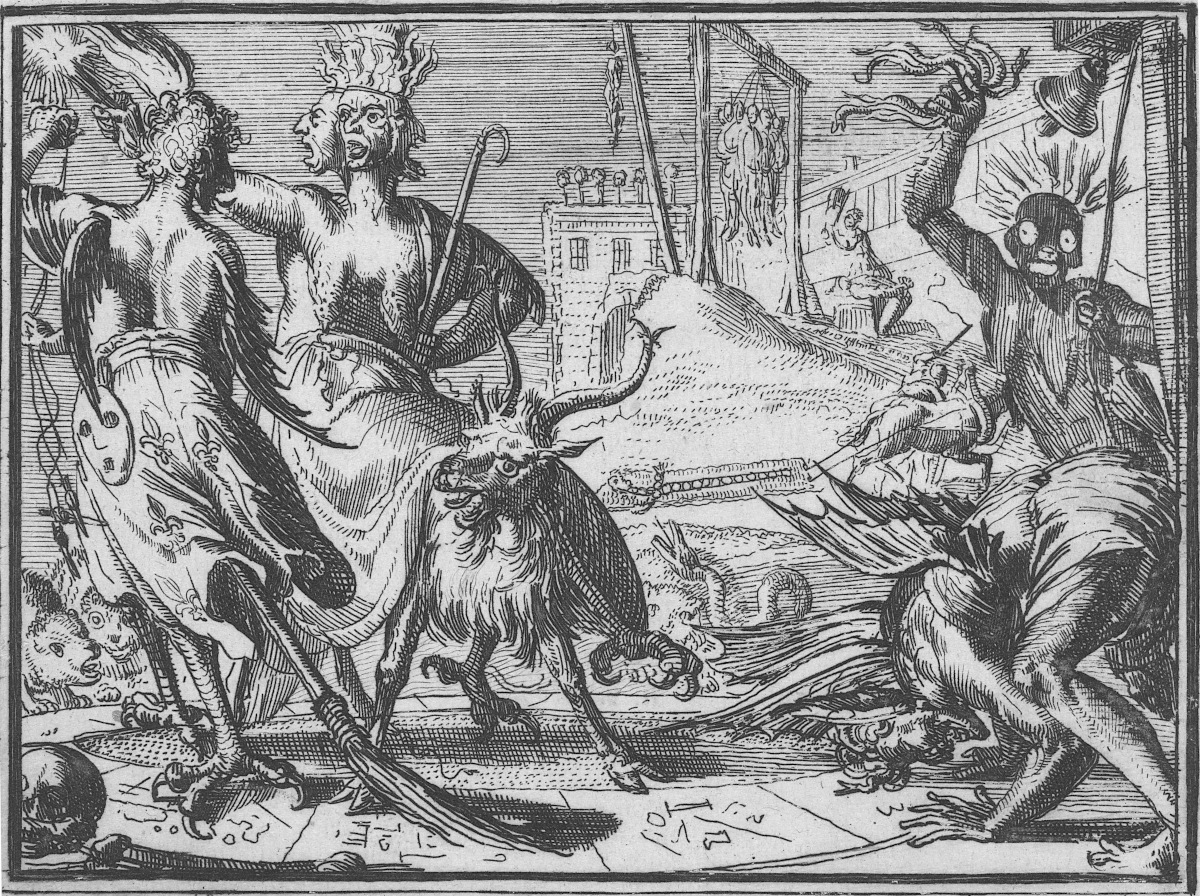
\includegraphics[keepaspectratio,width=\textwidth]{DeHorlende-small.jpg}
  \captionart{DeHorlendeKollendans}
  \label{fig:dehorlende}
\end{figure}

% Force float here
\clearpage{}
\thispagestyle{titleontop}

%SECT. II. MEMB. I. SUBSECT. III.-_Of Witches and Magicians, how they cause Melancholy_.
\section[Witches and Magicians]{Of Witches and Magicians, how they cause Melancholy.}

\lettrine{Y}{ou} have heard what the devil can do of himself, now you shall hear
what he can perform by his instruments, who are many times worse (if it
be possible) than he himself, and to satisfy their revenge and lust
cause more mischief, \li{Multa enim mala non egisset daemon, nisi
provocatus a sagis}, as Erastus thinks\authorfootnote{1252}; much harm had never been
done, had he not been provoked by witches to it. He had not appeared in
Samuel's shape, if the Witch of Endor had let him alone; or represented
those serpents in Pharaoh's presence, had not the magicians urged him
unto it; \li{Nec morbos vel hominibus, vel brutis infligeret} (Erastus
maintains) \li{si sagae quiescerent}; men and cattle might go free, if the
witches would let him alone. Many deny witches at all, or if there be
any they can do no harm; of this opinion is Wierus, lib. 3. cap. 53. \textlatin{de
praestig. daem.} \Austin{} Lerchemer a Dutch writer, Biarmanus, Ewichius,
Euwaldus, our countryman Scot; with him in \Horace{},
\li{Somnia, terrores Magicos, miracula, sagas,
Nocturnos Lemures, portentaque Thessala risu
Excipiunt.}---

\begin{verse}
Say, can you laugh indignant at the schemes\\*
Of magic terrors, visionary dreams,\\*
Portentous wonders, witching imps of Hell,\\*
The nightly goblin, and enchanting spell?
\end{verse}

They laugh at all such stories; but on the contrary are most lawyers,
divines, physicians, philosophers, \Austin{}, Hemingius, Danaeus,
Chytraeus, Zanchius, Aretius, \etc{}. Delrio, Springer, \authorfootnote{1253}Niderius,
lib. 5. Fornicar. Guiatius, Bartolus, consil. 6. tom. 1. Bodine,
daemoniant. lib 2. cap. 8. Godelman, Damhoderius, \etc{}. Paracelsus,
Erastus, Scribanius, Camerarius, \etc{}. The parties by whom the devil
deals, may be reduced to these two, such as command him in show at
least, as conjurors, and magicians, whose detestable and horrid
mysteries are contained in their book called \authorfootnote{1254}Arbatell; \li{daemonis
enim advocati praesto sunt, seque exorcismis et conjurationibus quasi
cogi patiuntur, ut miserum magorum genus, in impietate detineant.} Or
such as are commanded, as witches, that deal \li{ex parte} implicite, or
explicite, as the king\authormarginnote{1255} hath well defined; many subdivisions there
are, and many several species of sorcerers, witches, enchanters,
charmers, \etc{}. They have been tolerated heretofore some of them; and
magic hath been publicly professed in former times, in Salamanca\authormarginnote{1256},
Krakow\authormarginnote{1257}[2\baselineskip], and other places, though after censured by several
Universities\authormarginnote{1258}[3\baselineskip], and now generally contradicted, though practised by
some still, maintained and excused, \li{Tanquam res secreta quae non nisi
viris magnis et peculiari beneficio de Coelo instructis communicatur} (I
use \authorfootnote{1259}Boesartus his words) and so far approved by some princes, \li{Ut
nihil ausi aggredi in politicis, in sacris, in consiliis, sine eorum
arbitrio}; they consult still with them, and dare indeed do nothing
without their advice. Nero and Heliogabalus, Maxentius, and Julianus
Apostata, were never so much addicted to magic of old, as some of our
modern princes and popes themselves are nowadays. Erricus, King of
Sweden, had an \authorfootnote{1260}enchanted cap, by virtue of which, and some
magical murmur or whispering terms, he could command spirits, trouble
the air, and make the wind stand which way he would, insomuch that when
there was any great wind or storm, the common people were wont to say,
the king now had on his conjuring cap. But such examples are infinite.
That which they can do, is as much almost as the devil himself, who is
still ready to satisfy their desires, to oblige them the more unto him.
They can cause tempests, storms, which is familiarly practised by
witches in Norway, Iceland, as I have proved. They can make friends
enemies, and enemies friends by philters; \authorfootnote{1261}Turpes amores
conciliare, enforce love, tell any man where his friends are, about
what employed, though in the most remote places; and if they will,
\authorfootnote{1262}bring their sweethearts to them by night, upon a goat's back
flying in the air. Sigismund Scheretzius, part. 1. cap. 9. de spect.
reports confidently, that he conferred with sundry such, that had been
so carried many miles, and that he heard witches themselves confess as
much; hurt and infect men and beasts, vines, corn, cattle, plants, make
women abortive, not to conceive, \authorfootnote{1263}barren, men and women unapt and
unable, married and unmarried, fifty several ways, saith Bodine, lib.
2. c. 2. fly in the air, meet when and where they will, as Cicogna
proves, and Lavat. \textlatin{de spec}. part. 2. c. 17. steal young children out of
their cradles, \li{ministerio daemonum}, and put deformed in their rooms,
which we call changelings, saith \authorfootnote{1264}Scheretzius, part. 1. c. 6. make
men victorious, fortunate, eloquent; and therefore in those ancient
monomachies and combats they were searched of old, \authorfootnote{1265}they had no
magical charms; they can make \authorfootnote{1266}stick frees, such as shall endure a
rapier's point, musket shot, and never be wounded: of which read more
in Boissardus, cap. 6. de Magia, the manner of the adjuration, and by
whom 'tis made, where and how to be used in expeditionibus bellicis,
praeliis, duellis, \etc{}, with many peculiar instances and examples; they
can walk in fiery furnaces, make men feel no pain on the rack, aut
alias torturas sentire; they can stanch blood, \authorfootnote{1267}represent dead
men's shapes, alter and turn themselves and others into several forms,
at their pleasures. \authorfootnote{1268}Agaberta, a famous witch in Lapland, would do
as much publicly to all spectators, Modo Pusilla, modo anus, modo
procera ut quercus, modo vacca, avis, coluber, \etc{}. Now young, now old,
high, low, like a cow, like a bird, a snake, and what not? She could
represent to others what forms they most desired to see, show them
friends absent, reveal secrets, maxima omnium admiratione, \etc{}. And yet
for all this subtlety of theirs, as Lipsius well observes, Physiolog.
Stoicor. lib. 1. cap. 17. neither these magicians nor devils themselves
can take away gold or letters out of mine or Crassus' chest, et
Clientelis suis largiri, for they are base, poor, contemptible fellows
most part; as Bodine notes\authorfootnote{1269}, they can do nothing in Judicum
decreta aut poenas, in regum concilia vel arcana, nihil in rem
nummariam aut thesauros, they cannot give money to their clients, alter
judges' decrees, or councils of kings, these minuti Genii cannot do it,
altiores Genii hoc sibi adservarunt, the higher powers reserve these
things to themselves. Now and then peradventure there may be some more
famous magicians like Simon Magus, \authorfootnote{1270}Apollonius Tyaneus, Pasetes,
Jamblichus, \authorfootnote{1271}Odo de Stellis, that for a time can build castles in
the air, represent armies, \etc{}, as they are \authorfootnote{1272}said to have done,
command wealth and treasure, feed thousands with all variety of meats
upon a sudden, protect themselves and their followers from all princes'
persecutions, by removing from place to place in an instant, reveal
secrets, future events, tell what is done in far countries, make them
appear that died long since, and do many such miracles, to the world's
terror, admiration and opinion of deity to themselves, yet the devil
forsakes them at last, they come to wicked ends, and raro aut nunquam
such impostors are to be found. The vulgar sort of them can work no
such feats. But to my purpose, they can, last of all, cure and cause
most diseases to such as they love or hate, and this of
\authorfootnote{1273}melancholy amongst the rest. Paracelsus, Tom. 4. de morbis
amentium, Tract. 1. in express words affirms; Multi fascinantur in
melancholiam, many are bewitched into melancholy, out of his
experience. The same saith Danaeus, lib. 3. de sortiariis. Vidi,
inquit, qui Melancholicos morbos gravissimos induxerunt: I have seen
those that have caused melancholy in the most grievous manner,
\authorfootnote{1274}dried up women's paps, cured gout, palsy; this and apoplexy,
falling sickness, which no physic could help, solu tactu, by touch
alone. Ruland in his 3 Cent. Cura 91. gives an instance of one David
Helde, a young man, who by eating cakes which a witch gave him, mox
delirare coepit, began to dote on a sudden, and was instantly mad: F.
H. D. in \authorfootnote{1275}Hildesheim, consulted about a melancholy man, thought
his disease was partly magical, and partly natural, because he vomited
pieces of iron and lead, and spake such languages as he had never been
taught; but such examples are common in Scribanius, Hercules de
Saxonia, and others. The means by which they work are usually charms,
images, as that in Hector Boethius of King Duffe; characters stamped of
sundry metals, and at such and such constellations, knots, amulets,
words, philters, \etc{}, which generally make the parties affected,
melancholy; as Monavius discourseth\authorfootnote{1276} at large in an epistle of his
to Acolsius, giving instance in a Bohemian baron that was so troubled
by a philter taken. Not that there is any power at all in those spells,
charms, characters, and barbarous words; but that the devil doth use
such means to delude them. \li{Ut fideles inde magos} (saith Libanius\authormarginnote{1277})
\li{in officio retineat, tum in consortium malefactorum vocet.}

\cleartoleftpage{}
\begin{figure}[p]
  \begingroup
  \centering
  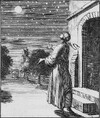
\includegraphics[keepaspectratio,width=\textwidth]{Woman-stars-small.jpg}
  \captionart{WomanStars}
  \label{fig:womanstars}
\end{figure}

% Force float here
\clearpage{}
\thispagestyle{titleontop}

%SECT. II. MEMB. I. SUBSECT. IV.-_Stars a cause. Signs from Physiognomy, Metoposcopy, Chiromancy_.
\section[Heavens, Planets, Stars]{Stars a cause. Signs from Physiognomy, Metoposcopy, Chiromancy.}\label{sec:heavens-planets-stars}

\lettrine{N}{atural} causes are either primary and universal, or secondary and more
particular. Primary causes are the heavens, planets, stars, \etc{}, by
their influence (as our astrologers hold) producing this and such like
effects. I will not here stand to discuss obiter, whether stars be
causes, or signs; or to apologise for judical astrology. If either
Sextus Empericus, Picus Mirandula, Sextus ab Heminga, Pererius,
Erastus, Chambers, \etc{}, have so far prevailed with any man, that he
will attribute no virtue at all to the heavens, or to sun, or moon,
more than he doth to their signs at an innkeeper's post, or tradesman's
shop, or generally condemn all such astrological aphorisms approved by
experience: I refer him to Bellantius, Pirovanus, Marascallerus,
Goclenius, Sir Christopher Heidon, \etc{}. If thou shalt ask me what I
think, I must answer, \lit{for I am conversant with these learned errors}{nam et doctis hisce erroribus versatus sum}, they do incline, but not
compel; no necessity at all: \li{agunt non cogunt}:\authormarginnote{1278} and so gently
incline, that a wise man may resist them; \li{sapiens dominabitur astris}:
they rule us, but God rules them. All this (methinks) \authorfootnote{1279}Joh. de
Indagine hath comprised in brief, \li{Quaeris a me quantum in nobis
operantur astra?} \etc{}. Wilt thou know how far the stars work upon us? I
say they do but incline, and that so gently, that if we will be ruled
by reason, they have no power over us; but if we follow our own nature,
and be led by sense, they do as much in us as in brute beasts, and we
are no better. So that, I hope, I may justly conclude with
Cajetan\authorfootnote{1280}, \li{Coelum est vehiculum divinae virtutis}, \etc{}, that the
heaven is God's instrument, by mediation of which he governs and
disposeth these elementary bodies; or a great book, whose letters are
the stars (as one calls it), wherein are written many strange things
for such as can read, or an excellent harp\authorfootnote{1281}, made by an eminent
workman, on which, he that can but play, will make most admirable
music. But to the purpose.

Paracelsus is of opinion\authorfootnote{1282}, that a physician without the knowledge
of stars can neither understand the cause or cure of any disease,
either of this or gout, not so much as toothache; except he see the
peculiar geniture and scheme of the party effected. And for this proper
malady, he will have the principal and primary cause of it proceed from
the heaven, ascribing more to stars than humours, and that the
constellation alone many times produceth melancholy\authorfootnote{1283}, all other causes
set apart. He gives instance in lunatic persons, that are deprived of
their wits by the moon's motion; and in another place refers all to the
ascendant, and will have the true and chief cause of it to be sought
from the stars. Neither is it his opinion only, but of many Galenists
and philosophers, though they do not so peremptorily maintain as much.
This variety of melancholy symptoms proceeds from the stars, saith
\authorfootnote{1284}Melancthon: the most generous melancholy, as that of Augustus,
comes from the conjunction of Saturn and Jupiter in Libra: the bad, as
that of Catiline's, from the meeting of Saturn and the moon in Scorpio.
Jovianus Pontanus, in his tenth book, and thirteenth chapter de rebus
coelestibus, discourseth to this purpose at large, Ex atra bile varii
generantur morbi, \etc{}, \authorfootnote{1285}many diseases proceed from black choler,
as it shall be hot or cold; and though it be cold in its own nature,
yet it is apt to be heated, as water may be made to boil, and burn as
bad as fire; or made cold as ice: and thence proceed such variety of
symptoms, some mad, some solitary, some laugh, some rage, \etc{}.

\begin{figure}[p]
  \begingroup
  \centering
  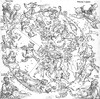
\includegraphics[keepaspectratio,width=\textwidth]{SkyMap-small.jpg}
  \captionart{SkyMap}
  \label{fig:skymap}
\end{figure}

The cause of all which intemperance he will have chiefly and primarily proceed
from the heavens, \authorfootnote{1286}from the position of Mars, Saturn, and Mercury.
His aphorisms be these, \authorfootnote{1287}Mercury in any geniture, if he shall be
found in Virgo, or Pisces his opposite sign, and that in the horoscope,
irradiated by those quartile aspects of Saturn or Mars, the child shall
be mad or melancholy. Again, \authorfootnote{1288}He that shall have Saturn and Mars,
the one culminating, the other in the fourth house, when he shall be
born, shall be melancholy, of which he shall be cured in time, if
Mercury behold them. If the moon be in conjunction or opposition\authorfootnote{1289}
at the birth time with the sun, Saturn or Mars, or in a quartile aspect
with them (\li{e malo coeli loco}, Leovitius adds), many diseases are
signified, especially the head and brain is like to be misaffected with
pernicious humours, to be melancholy, lunatic, or mad, Cardan adds,
quarta luna natos, eclipses, earthquakes. Garcaeus and Leovitius will
have the chief judgment to be taken from the lord of the geniture, or
where there is an aspect between the moon and Mercury, and neither
behold the horoscope, or Saturn and Mars shall be lord of the present
conjunction or opposition in Sagittarius or Pisces, of the sun or moon,
such persons are commonly epileptic, dote, demoniacal, melancholy: but
see more of these aphorisms in the above-named Pontanus. Garcaeus, cap.
23. de Jud. genitur. Schoner. lib. 1. cap. 8, which he hath gathered
out of \authorfootnote{1290}Ptolemy, Albubater, and some other Arabians, Junctine,
Ranzovius, Lindhout, Origen, \etc{}. But these men you will reject
peradventure, as astrologers, and therefore partial judges; then hear
the testimony of physicians, Galenists themselves. \authorfootnote{1291}Carto
confesseth the influence of stars to have a great hand to this peculiar
disease, so doth Jason Pratensis, Lonicerius praefat. de Apoplexia,
Ficinus, Fernelius, \etc{}. \authorfootnote{1292}P. Cnemander acknowledgeth the stars an
universal cause, the particular from parents, and the use of the six
non-natural things. Baptista Port. mag. l. 1. c. 10, 12, 15, will have
them causes to every particular individium. Instances and examples, to
evince the truth of those aphorisms, are common amongst those
astrologian treatises. Cardan, in his thirty-seventh geniture, gives
instance in Matth. Bolognius. Camerar. hor. natalit. centur. 7. genit.
6. et 7. of Daniel Gare, and others; but see Garcaeus, cap. 33. Luc.
Gauricus, Tract. 6. de Azemenis, \etc{}. The time of this melancholy is,
when the significators of any geniture are directed according to art,
as the hor: moon, hylech, \etc{} to the hostile beams or terms of \saturn{} and \mars{}
especially, or any fixed star of their nature, or if \saturn{} by his
revolution or transitus, shall offend any of those radical promissors
in the geniture.

Other signs there are taken from physiognomy, metoposcopy, chiromancy,
which because Joh. de Indagine, and Rotman, the landgrave of Hesse his
mathematician, not long since in his Chiromancy; Baptista Porta, in his
celestial Physiognomy, have proved to hold great affinity with
astrology, to satisfy the curious, I am the more willing to insert.
The general notions \authorfootnote{1293}physiognomers give, be these; black colour
argues natural melancholy; so doth leanness, hirsuteness, broad veins,
much hair on the brows, saith \authorfootnote{1294}Gratanarolus, cap. 7, and a little
head, out of \Aristotle, high sanguine, red colour, shows head
melancholy; they that stutter and are bald, will be soonest melancholy (as \Avicenna{} supposeth), by reason of the dryness of their brains; but
he that will know more of the several signs of humour and wits out of
physiognomy, let him consult with old Adamantus and Polemus, that
comment, or rather paraphrase upon \Aristotle's Physiognomy, Baptista
Porta's four pleasant books, Michael Scot de secretis naturae, John de
Indagine, Montaltus, Antony Zara. anat. ingeniorum, sect. 1. memb. 13.
et lib. 4. Chiromancy hath these aphorisms to foretell melancholy, Tasneir. lib.
5. cap. 2, who hath comprehended the sum of John de Indagine:
Tricassus, Corvinus, and others in his book, thus hath it; \authorfootnote{1295}The
Saturnine line going from the rascetta through the hand, to Saturn's
mount, and there intersected by certain little lines, argues
melancholy; so if the vital and natural make an acute angle, Aphorism
100. The saturnine, hepatic, and natural lines, making a gross triangle
in the hand, argue as much; which Goclenius, cap. 5. Chiros. repeats
verbatim out of him. In general they conclude all, that if Saturn's
mount be full of many small lines and intersections, \authorfootnote{1296}such men are
most part melancholy, miserable and full of disquietness, care and
trouble, continually vexed with anxious and bitter thoughts, always
sorrowful, fearful, suspicious; they delight in husbandry, buildings,
pools, marshes, springs, woods, walks, \etc{}. Thaddaeus Haggesius, in his
Metoposcopia, hath certain aphorisms derived from Saturn's lines in the
forehead, by which he collects a melancholy disposition; and
\authorfootnote{1297}Baptista Porta makes observations from those other parts of the
body, as if a spot be over the spleen; \authorfootnote{1298}or in the nails; if it
appear black, it signifieth much care, grief, contention, and
melancholy; the reason he refers to the humours, and gives instance in
himself, that for seven years space he had such black spots in his
nails, and all that while was in perpetual lawsuits, controversies for
his inheritance, fear, loss of honour, banishment, grief, care, \etc{} and
when his miseries ended, the black spots vanished. Cardan, in his book
de libris propriis, tells such a story of his own person, that a little
before his son's death, he had a black spot, which appeared in one of
his nails; and dilated itself as he came nearer to his end. But I am
over tedious in these toys, which howsoever, in some men's too severe
censures, they may be held absurd and ridiculous, I am the bolder to
insert, as not borrowed from circumforanean rogues and gipsies, but out
of the writings of worthy philosophers and physicians, yet living some
of them, and religious professors in famous universities, who are able
to patronise that which they have said, and vindicate themselves from
all cavillers and ignorant persons.

%SECT. II. MEMB. I. SUBSECT. V.-_Old age a cause_.
\section{Old age a cause.}

\lettrine{S}{econdary} peculiar causes efficient, so called in respect of the other
precedent, are either congenitae, internae, innatae, as they term them,
inward, innate, inbred; or else outward and adventitious, which happen
to us after we are born: congenite or born with us, are either natural,
as old age, or praeter naturam (as Fernelius calls\authorfootnote{1299} it) that
distemperature, which we have from our parent's seed, it being an
hereditary disease. The first of these, which is natural to all, and
which no man living can avoid, is \authorfootnote{1300}old age, which being cold and
dry, and of the same quality as melancholy is, must needs cause it, by
diminution of spirits and substance, and increasing of adust humours;
therefore \authorfootnote{1301} Melancthon avers out of \Aristotle, as an undoubted
truth, Senes plerunque delirasse in senecta, that old men familiarly
dote, ob atram bilem, for black choler, which is then superabundant in
them: and Rhasis, that Arabian physician, in his Cont. lib. 1. cap. 9,
calls it \authorfootnote{1302}a necessary and inseparable accident, to all old and
decrepit persons. After seventy years (as the Psalmist saith) \authorfootnote{1303}all
is trouble and sorrow; and common experience confirms the truth of it
in weak and old persons, especially such as have lived in action all
their lives, had great employment, much business, much command, and
many servants to oversee, and leave off ex abrupto; as Charles
the Fifth did\authorfootnote{1304} to King Philip, resign up all on a sudden; they are
overcome with melancholy in an instant: or if they do continue in such
courses, they dote at last (\li{senex bis puer}), and are not able to
manage their estates through common infirmities incident in their age;
full of ache, sorrow and grief, children again, dizzards, they carl
many times as they sit, and talk to themselves, they are angry,
waspish, displeased with every thing, suspicious of all, wayward,
covetous, hard (saith Tully), self-willed, superstitious,
self-conceited, braggers and admirers of themselves, as Balthazar
Castilio hath truly noted\authorfootnote{1305} of them.\authorfootnote{1306}This natural infirmity is most
eminent in old women, and such as are poor, solitary, live in most base
esteem and beggary, or such as are witches; insomuch that Wierus,
Baptista Porta, Ulricus Molitor, Edwicus, do refer all that witches are
said to do, to imagination alone, and this humour of melancholy. And
whereas it is controverted, whether they can bewitch cattle to death,
ride in the air upon a cowl-staff out of a chimney-top, transform
themselves into cats, dogs, \etc{}, translate bodies from place to place,
meet in companies, and dance, as they do, or have carnal copulation
with the devil, they ascribe all to this redundant melancholy, which
domineers in them, to \authorfootnote{1307} somniferous potions, and natural causes,
the devil's policy. Non laedunt omnino (saith Wierus) aut quid mirum
faciunt, (de Lamiis, lib. 3. cap. 36), ut putatur, solam vitiatam
habent phantasiam; they do no such wonders at all, only their
\authorfootnote{1308}brains are crazed. \authorfootnote{1309}They think they are witches, and can do
hurt, but do not. But this opinion Bodine, Erastus, Danaeus,
Scribanius, Sebastian Michaelis, \idxname{campanella}[Campanella][\textlatin{De sensu rerum et magia}] \textlatin{de Sensu rerum}, lib. 4.
cap. 9. \authorfootnote{1310}Dandinus the Jesuit, lib. 2. de Animae explode;
\authorfootnote{1311}Cicogna confutes at large. That witches are melancholy, they deny
not, but not out of corrupt phantasy alone, so to delude themselves and
others, or to produce such effects.

%SECT. II. MEMB. I. SUBSECT. VI.-_Parents a cause by Propagation_.
\section{Parents a cause by Propagation.}

\lettrine{T}{hat} other inward inbred cause of Melancholy is our temperature, in
whole or part, which we receive from our parents, which \authorfootnote{1312}Fernelius
calls Praeter naturam, or unnatural, it being an hereditary disease;
for as he justifies \authorfootnote{1313}Quale parentum maxime patris semen obtigerit,
tales evadunt similares spermaticaeque paries, quocunque etiam morbo
Pater quum generat tenetur, cum semine transfert, in Prolem; such as
the temperature of the father is, such is the son's, and look what
disease the father had when he begot him, his son will have after him;
\authorfootnote{1314}and is as well inheritor of his infirmities, as of his lands. And
where the complexion and constitution of the father is corrupt, there
(\authorfootnote{1315}saith Roger Bacon) the complexion and constitution of the son
must needs be corrupt, and so the corruption is derived from the father
to the son. Now this doth not so much appear in the composition of the
body, according to that of Hippocrates, \authorfootnote{1316}in habit, proportion,
scars, and other lineaments; but in manners and conditions of the mind,
Et patrum in natos abeunt cum semine mores.
Seleucus had an anchor on his thigh, so had his posterity, as Trogus
records, lib. 15. Lepidus, in \Pliny{} l. 7. c. 17, was purblind, so was
his son. That famous family of Aenobarbi were known of old, and so
surnamed from their red beards; the Austrian lip, and those Indian flat
noses are propagated, the Bavarian chin, and goggle eyes amongst the
Jews, as Buxtorfius observes\authorfootnote{1317}; their voice, pace, gesture, looks,
are likewise derived with all the rest of their conditions and
infirmities; such a mother, such a daughter; their very
\authorfootnote{1318}affections Lemnius contends to follow their seed, and the malice
and bad conditions of children are many times wholly to be imputed to
their parents; I need not therefore make any doubt of Melancholy, but
that it is an hereditary disease. \authorfootnote{1319} Paracelsus in express words
affirms it, lib. de morb. amentium to. 4. tr. 1; so doth \authorfootnote{1320}Crato in
an Epistle of his to Monavius. So doth Bruno Seidelius in his book de
morbo incurab. Montaltus proves, cap. 11, out of Hippocrates and
Plutarch, that such hereditary dispositions are frequent, et hanc
(inquit) fieri reor ob participatam melancholicam intemperantiam
(speaking of a patient) I think he became so by participation of
Melancholy. Daniel Sennertus, lib. 1. part 2. cap. 9, will have his
melancholy constitution derived not only from the father to the son,
but to the whole family sometimes; Quandoque totis familiis
hereditativam, \authorfootnote{1321}Forestus, in his medicinal observations,
illustrates this point, with an example of a merchant, his patient,
that had this infirmity by inheritance; so doth Rodericus a Fonseca,
tom. 1. consul. 69, by an instance of a young man that was so affected
ex matre melancholica, had a melancholy mother, et victu melancholico,
and bad diet together. Ludovicus Mercatus, a Spanish physician, in that
excellent Tract which he hath lately written of hereditary diseases,
tom. 2. oper. lib. 5, reckons up leprosy, as those \authorfootnote{1322}Galbots in
Gascony, hereditary lepers, pox, stone, gout, epilepsy, \etc{}. Amongst the
rest, this and madness after a set time comes to many, which he calls a
miraculous thing in nature, and sticks for ever to them as an incurable
habit. And that which is more to be wondered at, it skips in some
families the father, and goes to the son, \authorfootnote{1323}or takes every other,
and sometimes every third in a lineal descent, and doth not always
produce the same, but some like, and a symbolizing disease. These
secondary causes hence derived, are commonly so powerful, that (as
\authorfootnote{1324}Wolfius holds) saepe mutant decreta siderum, they do often alter
the primary causes, and decrees of the heavens. For these reasons,
belike, the Church and commonwealth, human and Divine laws, have
conspired to avoid hereditary diseases, forbidding such marriages as
are any whit allied; and as Mercatus adviseth all families to take
such, si fieri possit quae maxime distant natura, and to make choice of
those that are most differing in complexion from them; if they love
their own, and respect the common good. And sure, I think, it hath been
ordered by God's especial providence, that in all ages there should be
(as usually there is) once in \authorfootnote{1325}600 years, a transmigration of
nations, to amend and purify their blood, as we alter seed upon our
land, and that there should be as it were an inundation of those
northern Goths and Vandals, and many such like people which came out of
that continent of Scandia and Sarmatia (as some suppose) and overran,
as a deluge, most part of Europe and Africa, to alter for our good, our
complexions, which were much defaced with hereditary infirmities, which
by our lust and intemperance we had contracted. A sound generation of
strong and able men were sent amongst us, as those northern men usually
are, innocuous, free from riot, and free from diseases; to qualify and
make us as those poor naked Indians are generally at this day; and
those about Brazil (as a late \authorfootnote{1326}writer observes), in the Isle of
Maragnan, free from all hereditary diseases, or other contagion,
whereas without help of physic they live commonly 120 years or more, as
in the Orcades and many other places. Such are the common effects of
temperance and intemperance, but I will descend to particular, and show
by what means, and by whom especially, this infirmity is derived unto
us.

\li{Filii ex senibus nati, raro sunt firmi temperamenti}, old men's children
are seldom of a good temperament, as Scoltzius supposeth, consult. 177,
and therefore most apt to this disease; and as Levinus Lemnius
farther adds\authorfootnote{1327}, old men beget most part wayward, peevish, sad, melancholy
sons, and seldom merry. He that begets a child on a full stomach, will
either have a sick child, or a crazed son (as Cardan thinks\authorfootnote{1328}),
contradict. med. lib. 1. contradict. 18, or if the parents be sick, or
have any great pain of the head, or megrim, headache, (Hieronymus
Wolfius \authorfootnote{1329}doth instance in a child of Sebastian Castalio's); if a
drunken man get a child, it will never likely have a good brain, as
Gellius argues, lib. 12. cap. 1. Ebrii gignunt Ebrios, one drunkard
begets another, saith \authorfootnote{1330}Plutarch, symp. lib. 1. quest. 5, whose
sentence \authorfootnote{1331}Lemnius approves, l. 1. c. 4. Alsarius Crutius, Gen. de
qui sit med. cent. 3. fol. 182. Macrobius, lib. 1. \Avicenna{}, lib. 3.
Fen. 21. Tract 1. cap. 8, and \Aristotle himself, sect. 2. prob. 4,
foolish, drunken, or hair-brain women, most part bring forth children
like unto themselves, morosos et languidos, and so likewise he that
lies with a menstruous woman. Intemperantia veneris, quam in nautis
praesertim insectatur \authorfootnote{1332} Lemnius, qui uxores ineunt, nulla menstrui
decursus ratione habita nec observato interlunio, praecipua causa est,
noxia, pernitiosa, concubitum hunc exitialem ideo, et pestiferum vocat.
\authorfootnote{1333}Rodoricus a Castro Lucitanus, detestantur ad unum omnes medici,
tum et quarta luna concepti, infelices plerumque et amentes, deliri,
stolidi, morbosi, impuri, invalidi, tetra lue sordidi minime vitales,
omnibus bonis corporis atque animi destituti: ad laborem nati, si
seniores, inquit Eustathius, ut Hercules, et alii. \authorfootnote{1334}Judaei maxime
insectantur foedum hunc, et immundum apud Christianas Concubitum, ut
illicitum abhorrent, et apud suos prohibent; et quod Christiani toties
leprosi, amentes, tot morbili, impetigines, alphi, psorae, cutis et
faciei decolorationes, tam multi morbi epidemici, acerbi, et venenosi
sint, in hunc immundum concubitum rejiciunt, et crudeles in pignora
vocant, qui quarta, luna profluente hac mensium illuvie concubitum hunc
non perhorrescunt. Damnavit olim divina Lex et morte mulctavit
hujusmodi homines, Lev. 18, 20, et inde nati, siqui deformes aut
mutili, pater dilapidatus, quod non contineret ab \authorfootnote{1335} immunda
muliere. Gregorius Magnus, petenti Augustino nunquid apud
\authorfootnote{1336}Britannos hujusmodi concubitum toleraret, severe prohibuit viris
suis tum misceri foeminas in consuetis suis menstruis, \etc{}. I spare to
English this which I have said. Another cause some give, inordinate
diet, as if a man eat garlic, onions, fast overmuch, study too hard, be
over-sorrowful, dull, heavy, dejected in mind, perplexed in his
thoughts, fearful, \etc{}, their children (saith \authorfootnote{1337}Cardan subtil. lib.
18) will be much subject to madness and melancholy; for if the spirits
of the brain be fuzzled, or misaffected by such means, at such a time,
their children will be fuzzled in the brain: they will be dull, heavy,
timorous, discontented all their lives. Some are of opinion, and
maintain that paradox or problem, that wise men beget commonly fools;
Suidas gives instance in Aristarchus the Grammarian, duos reliquit
Filios Aristarchum et Aristachorum, ambos stultos; and which
\authorfootnote{1338}Erasmus urgeth in his Moria, fools beget wise men. Card. subt. l.
12, gives this cause, Quoniam spiritus sapientum ob studium
resolvuntur, et in cerebrum feruntur a corde: because their natural
spirits are resolved by study, and turned into animal; drawn from the
heart, and those other parts to the brain. Lemnius subscribes to that
of Cardan, and assigns this reason, Quod persolvant debitum languide,
et obscitanter, unde foetus a parentum generositate desciscit: they pay
their debt (as Paul calls it) to their wives remissly, by which means
their children are weaklings, and many times idiots and fools.
Some other causes are given, which properly pertain, and do proceed
from the mother: if she be over-dull, heavy, angry, peevish,
discontented, and melancholy, not only at the time of conception, but
even all the while she carries the child in her womb (saith Fernelius,
path. l. 1, 11) her son will be so likewise affected, and worse, as
\authorfootnote{1339}Lemnius adds, l. 4. c. 7, if she grieve overmuch, be disquieted,
or by any casualty be affrighted and terrified by some fearful object,
heard or seen, she endangers her child, and spoils the temperature of
it; for the strange imagination of a woman works effectually upon her
infant, that as Baptista Porta proves, Physiog. caelestis l. 5. c. 2,
she leaves a mark upon it, which is most especially seen in such as
prodigiously long for such and such meats, the child will love those
meats, saith Fernelius, and be addicted to like humours: \authorfootnote{1340}if a
great-bellied woman see a hare, her child will often have a harelip, as
we call it. Garcaeus, de Judiciis geniturarum, cap. 33, hath a
memorable example of one Thomas Nickell, born in the city of
Brandeburg, 1551, \authorfootnote{1341}that went reeling and staggering all the days
of his life, as if he would fall to the ground, because his mother
being great with child saw a drunken man reeling in the street. Such
another I find in Martin Wenrichius, com. de ortu monstrorum, c. 17, I
saw (saith he) at Wittenberg, in Germany, a citizen that looked like a
carcass; I asked him the cause, he replied, \authorfootnote{1342}His mother, when she
bore him in her womb, saw a carcass by chance, and was so sore
affrighted with it, that ex eo foetus ei assimilatus, from a ghastly
impression the child was like it.

So many several ways are we plagued and punished for our father's
defaults; insomuch that as Fernelius truly saith, \authorfootnote{1343}It is the
greatest part of our felicity to be well born, and it were happy for
human kind, if only such parents as are sound of body and mind should
be suffered to marry. An husbandman will sow none but the best and
choicest seed upon his land, he will not rear a bull or a horse, except
he be right shapen in all parts, or permit him to cover a mare, except
he be well assured of his breed; we make choice of the best rams for
our sheep, rear the neatest kine, and keep the best dogs, Quanto id
diligentius in procreandis liberis observandum? And how careful then
should we be in begetting of our children? In former times some
\authorfootnote{1344}countries have been so chary in this behalf, so stern, that if a
child were crooked or deformed in body or mind, they made him away; so
did the Indians of old by the relation of Curtius, and many other
well-governed commonwealths, according to the discipline of those
times. Heretofore in Scotland, saith \authorfootnote{1345}Hect. Boethius, if any were
visited with the falling sickness, madness, gout, leprosy, or any such
dangerous disease, which was likely to be propagated from the father to
the son, he was instantly gelded; a woman kept from all company of men;
and if by chance having some such disease, she were found to be with
child, she with her brood were buried alive: and this was done for the
common good, lest the whole nation should be injured or corrupted. A
severe doom you will say, and not to be used amongst Christians, yet
more to be looked into than it is. For now by our too much facility in
this kind, in giving way for all to marry that will, too much liberty
and indulgence in tolerating all sorts, there is a vast confusion of
hereditary diseases, no family secure, no man almost free from some
grievous infirmity or other, when no choice is had, but still the
eldest must marry, as so many stallions of the race; or if rich, be
they fools or dizzards, lame or maimed, unable, intemperate, dissolute,
exhaust through riot, as he said, \authorfootnote{1346}jura haereditario sapere
jubentur; they must be wise and able by inheritance: it comes to pass
that our generation is corrupt, we have many weak persons, both in body
and mind, many feral diseases raging amongst us, crazed families,
parentes, peremptores; our fathers bad, and we are like to be worse.

%SECT. II. MEMB. II.

%SECT. II. MEMB. II. SUBSECT. I.-_Bad Diet a cause. Substance. Quality of Meats_.
\section[Bad Diet]{Bad Diet a cause. Substance. Quality of Meats.}\label{sec:bad-diet}

\lettrine{A}{ccording} to my proposed method, having opened hitherto these secondary
causes, which are inbred with us, I must now proceed to the outward and
adventitious, which happen unto us after we are born. And those are
either evident, remote, or inward, antecedent, and the nearest:
continent causes some call them. These outward, remote, precedent
causes are subdivided again into necessary and not necessary. Necessary
(because we cannot avoid them, but they will alter us, as they are
used, or abused) are those six non-natural things, so much spoken of
amongst physicians, which are principal causes of this disease. For
almost in every consultation, whereas they shall come to speak of the
causes, the fault is found, and this most part objected to the patient;
Peccavit circa res sex non naturales: he hath still offended in one of
those six. Montanus, consil. 22, consulted about a melancholy Jew,
gives that sentence, so did Frisemelica in the same place; and in his
244 counsel, censuring a melancholy soldier, assigns that reason of his
malady, \authorfootnote{1347}he offended in all those six non-natural things, which
were the outward causes, from which came those inward obstructions; and
so in the rest.

These six non-natural things are diet, retention and evacuation, which
are more material than the other because they make new matter, or else
are conversant in keeping or expelling of it. The other four are air,
exercise, sleeping, waking, and perturbations of the mind, which only
alter the matter. The first of these is diet, which consists in meat
and drink, and causeth melancholy, as it offends in substance, or
accidents, that is, quantity, quality, or the like. And well it may be
called a material cause, since that, as Fernelius holds\authorfootnote{1348}, it hath
such a power in begetting of diseases, and yields the matter and
sustenance of them; for neither air, nor perturbations, nor any of
those other evident causes take place, or work this effect, except the
constitution of body, and preparation of humours, do concur. That a man
may say, this diet is the mother of diseases, let the father be what he
will, and from this alone, melancholy and frequent other maladies
arise. Many physicians, I confess, have written copious volumes of this
one subject, of the nature and qualities of all manner of meats; as
namely, Galen, Isaac the Jew, Halyabbas, \Avicenna{}, Mesue, also four
Arabians, Gordonius, Villanovanus, Wecker, Johannes Bruerinus,
sitologia de Esculentis et Poculentis, Michael Savanarola, Tract 2. c.
8, Anthony Fumanellus, lib. de regimine senum, Curio in his comment on
Schola Salerna, Godefridus Steckius arte med., Marcilius Cognatus,
Ficinus, Ranzovius, Fonseca, Lessius, Magninus, regim. sanitatis,
Frietagius, Hugo Fridevallius, \etc{}, besides many other in
\authorfootnote{1349}English, and almost every peculiar physician, discourseth at
large of all peculiar meats in his chapter of melancholy: yet because
these books are not at hand to every man, I will briefly touch what
kind of meats engender this humour, through their several species, and
which are to be avoided. How they alter and change the matter, spirits
first, and after humours, by which we are preserved, and the
constitution of our body, Fernelius and others will show you. I hasten
to the thing itself: and first of such diet as offends in substance.

\subsection{Beef.}
Beef, a strong and hearty meat (cold in the first degree, dry
in the second, saith \textlatin{Gal. l. 3. c. 1. de alim. fac.}) is condemned by
him and all succeeding Authors, to breed gross melancholy blood: good
for such as are sound, and of a strong constitution, for labouring men
if ordered aright, corned, young, of an ox (for all gelded meats in
every species are held best), or if old, \authorfootnote{1350}such as have been tired
out with labour, are preferred. Aubanus and Sabellicus commend Portugal
beef to be the most savoury, best and easiest of digestion; we commend
ours: but all is rejected, and unfit for such as lead a resty life, any
ways inclined to melancholy, or dry of complexion: \li{Tales} (Galen thinks)
\li{de facile melancholicis aegritudinibus capiuntur}.
\begin{figure}[H]
  \begingroup
  \centering
  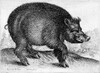
\includegraphics[keepaspectratio,width=\textwidth]{wild-boar-small.jpg}
  \captionart{WildBoar}
  \label{fig:wildboar}
\end{figure}
\subsection{Pork.}
Pork, of all meats, is most nutritive in his own nature,
\authorfootnote{1351} but altogether unfit for such as live at ease, are any ways
unsound of body or mind: too moist, full of humours, and therefore
\lit{naught for queasy stomachs, insomuch that frequent use of it may breed a quartan ague}{noxia delicatis, ex earum usu ut dubitetur an febris quartana generetur}, saith Savanarola.
\subsection{Goat.}
Savanarola discommends goat's flesh, and so doth
\authorfootnote{1352}\textlatin{Bruerinus, l. 13. c. 19}, calling it a filthy beast, and rammish:
and therefore supposeth it will breed rank and filthy substance; yet
kid, such as are young and tender, Isaac accepts, Bruerinus and Galen,
\textlatin{l. 1. c. 1. de alimentorum facultatibus.}
\subsection{Hart.}
\emph{Hart} and \emph{red deer} \authorfootnote{1353}hath an evil name: it yields gross
nutriment: a strong and great grained meat, next unto a horse. Which
although some countries eat, as Tartars, and they of China; yet \authorfootnote{1354}
Galen condemns. Young foals are as commonly eaten in Spain as red deer,
and to furnish their navies, about Malaga especially, often used; but
such meats ask long baking, or seething, to qualify them, and yet all
will not serve.

\emph{Venison, Fallow Deer}. All venison is melancholy, and begets bad blood;
a pleasant meat: in great esteem with us (for we have more parks in
England than there are in all Europe besides) in our solemn feasts.
'Tis somewhat better hunted than otherwise, and well prepared by
cookery; but generally bad, and seldom to be used.
\subsection{Hare.}
\emph{Hare}, a black meat, melancholy, and hard of digestion, it
breeds incubus, often eaten, and causeth fearful dreams, so doth all
venison, and is condemned by a jury of physicians. Mizaldus and some
others say, that hare is a merry meat, and that it will make one fair,
as Martial's epigram testifies to Gellia; but this is per accidens,
because of the good sport it makes, merry company and good discourse
that is commonly at the eating of it, and not otherwise to be
understood.

\subsection{Conies.}
\authorfootnote{1355}\emph{Conies} are of the nature of hares. Magninus compares
them to beef, pig, and goat, Reg. sanit. part. 3. c. 17; yet young
rabbits by all men are approved to be good.
Generally, all such meats as are hard of digestion breed melancholy.
Areteus, lib. 7. cap. 5, reckons up heads and feet, \authorfootnote{1356}bowels,
brains, entrails, marrow, fat, blood, skins, and those inward parts, as
heart, lungs, liver, spleen, \etc{}. They are rejected by Isaac, lib. 2.
part. 3, Magninus, part. 3. cap. 17, Bruerinus, lib. 12, Savanarola,
Rub. 32. Tract. 2.

\subsection{Milk.}
\emph{Milk}, and all that comes of milk, as butter and cheese, curds,
\etc{}, increase melancholy (whey only excepted, which is most wholesome):
\authorfootnote{1357}some except asses' milk. The rest, to such as are sound, is
nutritive and good, especially for young children, but because soon
turned to corruption, \authorfootnote{1358}not good for those that have unclean
stomachs, are subject to headache, or have green wounds, stone, \etc{}. Of
all cheeses, I take that kind which we call Banbury cheese to be the
best, ex vetustis pessimus, the older, stronger, and harder, the worst,
as Langius discourseth in his Epistle to Melancthon, cited by Mizaldus,
Isaac, p. 5. Gal. 3. de cibis boni succi. \etc{}.

\begin{figure}[H]
  \begingroup
  \centering
  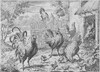
\includegraphics[keepaspectratio,width=\textwidth]{chickens-small.jpg}
  \captionart{Chickens}
  \label{fig:chickens}
\end{figure}

\subsection{Fowl.}
Amongst fowl, \authorfootnote{1359}peacocks and pigeons, all fenny fowl are
forbidden, as ducks, geese, swans, herons, cranes, coots, didappers,
water-hens, with all those teals, curs, sheldrakes, and peckled fowls,
that come hither in winter out of Scandia, Muscovy, Greenland,
Friesland, which half the year are covered all over with snow, and
frozen up. Though these be fair in feathers, pleasant in taste, and
have a good outside, like hypocrites, white in plumes, and soft, their
flesh is hard, black, unwholesome, dangerous, melancholy meat; Gravant
et putrefaciant stomachum, saith Isaac, part. 5. de vol., their young
ones are more tolerable, but young pigeons he quite disapproves.

\begin{figure}[H]
  \begingroup
  \centering
  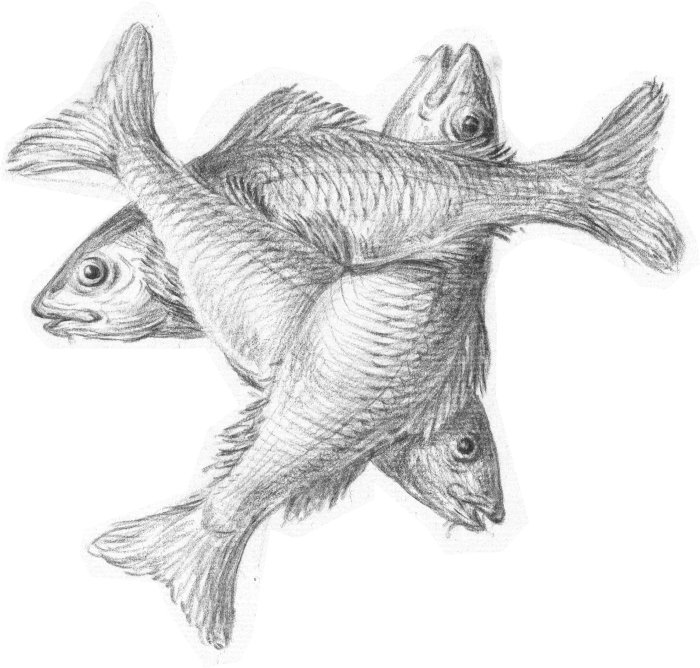
\includegraphics[keepaspectratio,width=0.7\textwidth]{Three-fishes-arranged-crosswise-small.jpg}
  \captionart{ThreeFishes}
  \label{fig:threefishes}
\end{figure}

\subsection{Fishes.}\label{sec:fishes}
Rhasis and \authorfootnote{1360}Magninus discommend all fish, and say, they
breed viscosities, slimy nutriment, little and humorous nourishment.
Savanarola adds, cold, moist: and phlegmatic, Isaac; and therefore
unwholesome for all cold and melancholy complexions: others make a
difference, rejecting only amongst freshwater fish, eel, tench,
lamprey, crawfish (which Bright approves, cap. 6), and such as are bred
in muddy and standing waters, and have a taste of mud, as Franciscus
Bonsuetus poetically defines, Lib. de aquatilibus.
%
\begin{latin}
\begin{verse}
Nam pisces omnes, qui stagna, lacusque frequentant,\\*
Semper plus succi deterioris habent.
\end{verse}
\end{latin}
\translationrule
\begin{verse}
All fish, that standing pools, and lakes frequent,\\*
Do ever yield bad juice and nourishment.
\end{verse}

Lampreys, Paulus Jovius, c. 34. de piscibus fluvial., highly magnifies,
and saith, None speak against them, but inepti et scrupulosi, some
scrupulous persons; but \authorfootnote{1361}eels, c. 33, he abhorreth in all places,
at all times, all physicians detest them, especially about the
solstice. Gomesius, lib. 1. c. 22, de sale, doth immoderately extol
sea-fish, which others as much vilify, and above the rest, dried,
soused, indurate fish, as ling, fumados, red-herrings, sprats,
stock-fish, haberdine, poor-John, all shellfish. \authorfootnote{1362}Tim. Bright
excepts lobster and crab. Messarius commends salmon, which Bruerinus
contradicts, lib. 22. c. 17. Magninus rejects conger, sturgeon, turbot,
mackerel, skate.

Carp is a fish of which I know not what to determine. Franciscus
Bonsuetus accounts it a muddy fish. Hippolitus Salvianus, in his Book
de Piscium natura et praeparatione, which was printed at Rome in folio,
1554, with most elegant pictures, esteems carp no better than a slimy
watery meat. Paulus Jovius on the other side, disallowing tench,
approves of it; so doth Dubravius in his Books of Fishponds. Freitagius
\authorfootnote{1363}extols it for an excellent wholesome meat, and puts it amongst
the fishes of the best rank; and so do most of our country gentlemen,
that store their ponds almost with no other fish. But this controversy
is easily decided, in my judgment, by Bruerinus, l. 22. c. 13. The
difference riseth from the site and nature of pools, \authorfootnote{1364}sometimes
muddy, sometimes sweet; they are in taste as the place is from whence
they be taken. In like manner almost we may conclude of other fresh
fish. But see more in Rondoletius, Bellonius, Oribasius, lib. 7. cap.
22, Isaac, l. 1, especially Hippolitus Salvianus, who is instar omnium
solus, \etc{}. Howsoever they may be wholesome and approved, much use of
them is not good; P. Forestus, in his medicinal observations,
\authorfootnote{1365}relates, that Carthusian friars, whose living is most part fish,
are more subject to melancholy than any other order, and that he found
by experience, being sometimes their physician ordinary at Delft, in
Holland. He exemplifies it with an instance of one Buscodnese, a
Carthusian of a ruddy colour, and well liking, that by solitary living,
and fish-eating, became so misaffected.

\subsection{Herbs.}
Amongst herbs to be eaten I find gourds, cucumbers,
coleworts, melons, disallowed, but especially cabbage. It causeth
troublesome dreams, and sends up black vapours to the brain. Galen,
loc. affect. l. 3. c. 6, of all herbs condemns cabbage; and Isaac, lib.
2. c. 1. Animae gravitatem facit, it brings heaviness to the soul. Some
are of opinion that all raw herbs and salads breed melancholy blood,
except bugloss and lettuce. Crato, consil. 21. lib. 2, speaks against
all herbs and worts, except borage, bugloss, fennel, parsley, dill,
balm, succory. Magninus, regim. sanitatis, part. 3. cap. 31. Omnes
herbae simpliciter malae, via cibi; all herbs are simply evil to feed
on (as he thinks). So did that scoffing cook in \authorfootnote{1366}\Plautus{} hold:
Non ego coenam condio ut alii coqui solent,
Qui mihi condita prata in patinis proferunt,
Boves qui convivas faciunt, herbasque aggerunt.


Like other cooks I do not supper dress,
That put whole meadows into a platter,

And make no better of their guests than beeves,
With herbs and grass to feed them fatter.

Our Italians and Spaniards do make a whole dinner of herbs and salads
(which our said \Plautus{} calls coenas terrestras, \Horace{}, coenas sine
sanguine), by which means, as he follows it,
\authorfootnote{1367}Hic homines tam brevem vitam colunt-
Qui herbas hujusmodi in alvum suum congerunt,
Formidolosum dictu, non esu modo,
Quas herbas pecudes non edunt, homines edunt.

Their lives, that eat such herbs, must needs be short,
And 'tis a fearful thing for to report,
That men should feed on such a kind of meat,
Which very juments would refuse to eat.

\authorfootnote{1368}They are windy, and not fit therefore to be eaten of all men raw,
though qualified with oil, but in broths, or otherwise. See more of
these in every \authorfootnote{1369}husbandman, and herbalist.
\subsection{Roots.}
Roots, Etsi quorundam gentium opes sint, saith Bruerinus, the
wealth of some countries, and sole food, are windy and bad, or
troublesome to the head: as onions, garlic, scallions, turnips,
carrots, radishes, parsnips: Crato, lib. 2. consil. 11, disallows all
roots, though \authorfootnote{1370} some approve of parsnips and potatoes.
\authorfootnote{1371}Magninus is of Crato's opinion, \authorfootnote{1372}They trouble the mind,
sending gross fumes to the brain, make men mad, especially garlic,
onions, if a man liberally feed on them a year together. Guianerius,
tract. 15. cap. 2, complains of all manner of roots, and so doth
Bruerinus, even parsnips themselves, which are the best, Lib. 9. cap.
14.
\subsection{Fruits.}
\li{Pastinacarum usus succos gignit improbos}. Crato, consil. 21.
lib. 1, utterly forbids all manner of fruits, as pears, apples, plums,
cherries, strawberries, nuts, medlars, serves, \etc{}. Sanguinem inficiunt,
saith Villanovanus, they infect the blood, and putrefy it, Magninus
holds, and must not therefore be taken via cibi, aut quantitate magna,
not to make a meal of, or in any great quantity. \authorfootnote{1373}Cardan makes
that a cause of their continual sickness at Fessa in Africa, because
they live so much on fruits, eating them thrice a day. Laurentius
approves of many fruits, in his \emph{Tract of Melancholy}, which others
disallow, and amongst the rest apples, which some likewise commend,
sweetings, pearmains, pippins, as good against melancholy; but to him
that is any way inclined to, or touched with this malady,
\authorfootnote{1374}Nicholas Piso in his \emph{Practics}, forbids all fruits, as windy, or
to be sparingly eaten at least, and not raw. Amongst other fruits,
\authorfootnote{1375}Bruerinus, out of Galen, excepts grapes and figs, but I find them
likewise rejected.

\subsection{Pulse.}
All \footnoteA{Dried legume. \theeditor{}}{pulse} are naught, beans, peas, vetches, \etc{}, they fill
the brain (saith Isaac) with gross fumes, breed black thick blood, and
cause troublesome dreams. And therefore, that which Pythagoras said to
his scholars of old, may be for ever applied to melancholy men, A fabis
abstinete, eat no peas, nor beans; yet to such as will needs eat them,
I would give this counsel, to prepare them according to those rules
that Arnoldus Villanovanus, and Frietagius prescribe, for eating, and
dressing. fruits, herbs, roots, pulse, \etc{}

\subsection{Spices.}
Spices cause hot and head melancholy, and are for that cause
forbidden by our physicians to such men as are inclined to this malady,
as pepper, ginger, cinnamon, cloves, mace, dates, \etc{} honey and sugar.
Some except honey;\authorfootnote{1376} to those that are cold, it may be tolerable,
but \latininlinetrans{sweets turn into bile}{Dulcia se in bilem vertunt},\authormarginnote{1377} they
are obstructive. Crato therefore forbids all spice, in a consultation
of his, for a melancholy schoolmaster, Omnia aromatica et quicquid
sanguinem adurit: so doth Fernelius, consil. 45. Guianerius, tract 15.
cap. 2. Mercurialis, cons. 189. To these I may add all sharp and sour
things, luscious and over-sweet, or fat, as oil, vinegar, verjuice,
mustard, salt; as sweet things are obstructive, so these are corrosive.
Gomesius, in his books, de sale, l. 1. c. 21, highly commends salt; so
doth Codronchus in his tract, de sale Absynthii, Lemn. l. 3. c. 9. de
occult. nat. mir. yet common experience finds salt, and salt-meats, to
be great procurers of this disease. And for that cause belike those
Egyptian priests abstained from salt, even so much, as in their bread,
ut sine perturbatione anima esset, saith mine author, that their souls
might be free from perturbations.

\subsection{Bread.}
Bread that is made of baser grain, as peas, beans, oats, rye,
or \authorfootnote{1378}over-hard baked, crusty, and black, is often spoken against,
as causing melancholy juice and wind. Joh. Mayor, in the first book of
his History of Scotland, contends much for the wholesomeness of oaten
bread: it was objected to him then living at Paris in France, that his
countrymen fed on oats, and base grain, as a disgrace; but he doth
ingenuously confess, Scotland, Wales, and a third part of England, did
most part use that kind of bread, that it was as wholesome as any
grain, and yielded as good nourishment. And yet Wecker out of Galen
calls it horsemeat, and fitter for juments than men to feed on. But
read Galen himself, Lib. 1. De cibis boni et mali succi, more largely
discoursing of corn and bread.

\subsection{Wine.}
All black wines, over-hot, compound, strong thick drinks, as
Muscadine, Malmsey, Alicant, Rumney, Brownbastard, Metheglen, and the
like, of which they have thirty several kinds in Muscovy, all such made
drinks are hurtful in this case, to such as are hot, or of a sanguine
choleric complexion, young, or inclined to head-melancholy. For many
times the drinking of wine alone causeth it. Arculanus, c. 16. in 9.
Rhasis, puts in \authorfootnote{1379}wine for a great cause, especially if it be
immoderately used. Guianerius, tract. 15. c. 2, tells a story of two
Dutchmen, to whom he gave entertainment in his house, that \authorfootnote{1380}in one
month's space were both melancholy by drinking of wine, one did nought
but sing, the other sigh. Galen, l. de causis morb. c. 3. Matthiolus on
Dioscorides, and above all other Andreas Bachius, l. 3. 18, 19, 20,
have reckoned upon those inconveniences that come by wine: yet
notwithstanding all this, to such as are cold, or sluggish melancholy,
a cup of wine is good physic, and so doth Mercurialis grant, consil.
25, in that case, if the temperature be cold, as to most melancholy men
it is, wine is much commended, if it be moderately used.
\subsection{Cider, Perry.}

Cider and perry are both cold and windy drinks, and
for that cause to be neglected, and so are all those hot spiced strong
drinks.

\paragraph{Beer} Beer, if it be over-new or over-stale, over-strong, or not
sodden, smell of the cask, sharp, or sour, is most unwholesome, frets,
and galls, \etc{}. Henricus Ayrerus, in a \authorfootnote{1381}consultation of his, for
one that laboured of hypochondriacal melancholy, discommends beer. So
doth \authorfootnote{1382} Crato in that excellent counsel of his, Lib. 2. consil. 21,
as too windy, because of the hop. But he means belike that thick black
Bohemian beer used in some other parts of \authorfootnote{1383}Germany.
---nil spissius illa
Dum bibitur, nil clarius est dum mingitur, unde
Constat, quod multas faeces in corpore linquat.

Nothing comes in so thick,
Nothing goes out so thin,
It must needs follow then
The dregs are left within.

As that \authorfootnote{1384}old poet scoffed, calling it Stygiae monstrum conforme
paludi, a monstrous drink, like the river Styx. But let them say as
they list, to such as are accustomed unto it, 'tis a most wholesome (so
\authorfootnote{1385} \idxname{polydorevergil}[Polydore Virgil] calleth it) and a pleasant drink, it is more
subtle and better, for the hop that rarefies it, hath an especial
virtue against melancholy, as our herbalists confess, Fuchsius
approves, Lib. 2. sec. 2. instit. cap. 11, and many others.

\paragraph{Waters} Standing waters, thick and ill-coloured, such as come forth of
pools, and moats, where hemp hath been steeped, or slimy fishes live,
are most unwholesome, putrefied, and full of mites, creepers, slimy,
muddy, unclean, corrupt, impure, by reason of the sun's heat, and
still-standing; they cause foul distemperatures in the body and mind of
man, are unfit to make drink of, to dress meat with, or to be
\authorfootnote{1386}used about men inwardly or outwardly. They are good for many
domestic uses, to wash horses, water cattle, \etc{}, or in time of
necessity, but not otherwise. Some are of opinion, that such fat
standing waters make the best beer, and that seething doth defecate it,
as Cardan holds\authorfootnote{1387}, Lib. 13. subtil. It mends the substance, and
savour of it, but it is a paradox. Such beer may be stronger, but not
so wholesome as the other, as Jobertus truly justifieth\authorfootnote{1388} out of
Galen, Paradox, dec. 1. Paradox 5, that the seething of such impure
waters doth not purge or purify them, \Pliny{}, lib. 31. c. 3, is of the
same tenet, and P. Crescentius, agricult. lib. 1. et lib. 4. c. 11. et
c. 45. Pamphilius Herilachus, l. 4. de not. aquarum, such waters are
naught, not to be used, and by the testimony of \authorfootnote{1389}Galen, breed
agues, dropsies, pleurisies, splenetic and melancholy passions, hurt
the eyes, cause a bad temperature, and ill disposition of the whole
body, with bad colour. This Jobertus stiffly maintains, Paradox, lib.
1. part. 5, that it causeth blear eyes, bad colour, and many loathsome
diseases to such as use it: this which they say, stands with good
reason; for as geographers relate, the water of Astracan breeds worms
in such as drink it. \authorfootnote{1390} Axius, or as now called Verduri, the
fairest river in Macedonia, makes all cattle black that taste of it.
Aleacman now Peleca, another stream in Thessaly, turns cattle most part
white, si polui ducas, L. Aubanus Rohemus refers that \authorfootnote{1391}struma or
poke of the Bavarians and Styrians to the nature of their waters, as
\authorfootnote{1392}Munster doth that of Valesians in the Alps, and \authorfootnote{1393}Bodine
supposeth the stuttering of some families in Aquitania, about Labden,
to proceed from the same cause, and that the filth is derived from the
water to their bodies. So that they that use filthy, standing,
ill-coloured, thick, muddy water, must needs have muddy, ill-coloured,
impure, and infirm bodies. And because the body works upon the mind,
they shall have grosser understandings, dull, foggy, melancholy
spirits, and be really subject to all manner of infirmities.

To these noxious simples, we may reduce an infinite number of compound,
artificial, made dishes, of which our cooks afford us a great variety,
as tailors do fashions in our apparel. Such are \authorfootnote{1394}puddings stuffed
with blood, or otherwise composed; baked, meats, soused indurate meats,
fried and broiled buttered meats; condite, powdered, and over-dried,
\authorfootnote{1395}all cakes, simnels, buns, cracknels made with butter, spice, \etc{},
fritters, pancakes, pies, sausages, and those several sauces, sharp, or
over-sweet, of which scientia popinae, as \Seneca calls it, hath served
those \authorfootnote{1396} Apician tricks, and perfumed dishes, which Adrian the
sixth Pope so much admired in the accounts of his predecessor Leo
Decimus; and which prodigious riot and prodigality have invented in
this age. These do generally engender gross humours, fill the stomach
with crudities, and all those inward parts with obstructions. Montanus,
consil. 22, gives instance, in a melancholy Jew, that by eating such
tart sauces, made dishes, and salt meats, with which he was overmuch
delighted, became melancholy, and was evil affected. Such examples are
familiar and common.

%SECT. II. MEMB. II. SUBSECT. II.-_Quantity of Diet a Cause._
\section{Quantity of Diet a Cause.}

\lettrine{T}{here} is not so much harm proceeding from the substance itself of meat,
and quality of it, in ill-dressing and preparing, as there is from the
quantity, disorder of time and place, unseasonable use of it, \authorfootnote{1397}
intemperance, overmuch, or overlittle taking of it. A true saying it
is, Plures crapula quam gladius. This gluttony kills more than the
sword, this omnivorantia et homicida gula, this all-devouring and
murdering gut. And that of \authorfootnote{1398}\Pliny{} is truer, Simple diet is the
best; heaping up of several meats is pernicious, and sauces worse; many
dishes bring many diseases. \authorfootnote{1399}Avicen cries out, That nothing is
worse than to feed on many dishes, or to protract the time of meats
longer than ordinary; from thence proceed our infirmities, and 'tis the
fountain of all diseases, which arise out of the repugnancy of gross
humours. Thence, saith \authorfootnote{1400} Fernelius, come crudities, wind,
oppilations, cacochymia, plethora, cachexia, bradiopepsia, \authorfootnote{1401}Hinc
subitae, mortes, atque intestata senectus, sudden death, \etc{}, and what
not.

As a lamp is choked with a multitude of oil, or a little fire with
overmuch wood quite extinguished, so is the natural heat with
immoderate eating, strangled in the body. Pernitiosa sentina est
abdomen insaturabile: one saith, An insatiable paunch is a pernicious
sink, and the fountain of all diseases, both of body and mind.
\authorfootnote{1402}Mercurialis will have it a peculiar cause of this private
disease; Solenander, consil. 5. sect. 3, illustrates this of
Mercurialis, with an example of one so melancholy, ab intempestivis
commessationibus, unseasonable feasting. \authorfootnote{1403}Crato confirms as much,
in that often cited counsel, 21. lib. 2, putting superfluous eating for
a main cause. But what need I seek farther for proofs? Hear
\authorfootnote{1404}Hippocrates himself, lib. 2. aphor. 10, Impure bodies the more
they are nourished, the more they are hurt, for the nourishment is
putrefied with vicious humours.

\begin{figure}[H]
  \begingroup
  \centering
  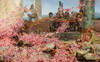
\includegraphics[keepaspectratio,width=\textwidth]{heliogabalus-small.jpg}
  \captionart{Heliogabalus}
  \label{fig:heliogabalus}
\end{figure}

And yet for all this harm, which apparently follows surfeiting and
drunkenness, see how we luxuriate and rage in this kind; read what
Johannes Stuckius hath written lately of this subject, in his great
volume De Antiquorum Conviviis, and of our present age; Quam
\authorfootnote{1405}portentosae coenae, prodigious suppers, \authorfootnote{1406}Qui dum invitant ad
coenam efferunt ad sepulchrum, what Fagos, Epicures, Apetios,
Heliogabalus, our times afford? Lucullus' ghost walks still,\footnoteA{\scriptsize{}Roman politician and famed gastronome. As recorded in Plutarch's Parallel Lives, on an occasion without dinner guests his servant prepared a plain course. Lucullus reprimanded him: \lit{What, did not you know, then, that today Lucullus dines with Lucullus?}{Quid ais, inquit iratus Lucullus, au nesciebas Lucullum hodie cenaturum esse apud Lucullum}. Plutarch, Life of Lucullus, 41.1–6.} and every
man desires to sup in Apollo; Aesop's costly dish is ordinarily served
up. \li{Magis illa juvant, quae pluris emuntur}\authorlatintrans{1407.5}.\authormarginnote{1407} The dearest cates are
best, and 'tis an ordinary thing to bestow twenty or thirty pounds on a
dish, some thousand crowns upon a dinner: \authorfootnote{1408}Mully-Hamet, king of
Fez and Morocco, spent three pounds on the sauce of a capon: it is
nothing in our times, we scorn all that is cheap. We loathe the very
\authorfootnote{1409}light (some of us, as \Seneca notes) because it comes free, and we
are offended with the sun's heat, and those cool blasts, because we buy
them not. This air we breathe is so common, we care not for it; nothing
pleaseth but what is dear. And if we be \authorfootnote{1410}witty in anything, it is
ad gulam: If we study at all, it is erudito luxu, to please the palate,
and to satisfy the gut. A cook of old was a base knave (as Livy
complains\authorfootnote{1411}), but now a great man in request; cookery is become an art, a
noble science: cooks are gentlemen: Venter Deus: They wear their brains
in their bellies, and their guts in their heads, as Agrippa taxed\authorfootnote{1412}
some parasites of his time, rushing on their own destruction, as if a
man should run upon the point of a sword, usque dum rumpantur comedunt,

They eat till they burst: \authorfootnote{1413}All day, all night, let the physician
say what he will, imminent danger, and feral diseases are now ready to
seize upon them, that will eat till they vomit, Edunt ut vomant, vomut
ut edant, saith \Seneca; which Dion relates of Vitellius, Solo transitu
ciborum nutriri judicatus: His meat did pass through and away, or till
they burst again. \authorfootnote{1414}Strage animantium ventrem onerant, and rake
over all the world, as so many \authorfootnote{1415}slaves, belly-gods, and
land-serpents, Et totus orbis ventri nimis angustus, the whole world
cannot satisfy their appetite. \authorfootnote{1416}Sea, land, rivers, lakes, \etc{}, may
not give content to their raging guts. To make up the mess, what
immoderate drinking in every place? Senem potum pota trahebat anus, how
they flock to the tavern: as if they were fruges consumere nati, born
to no other end but to eat and drink, like Offellius Bibulus, that
famous Roman parasite, Qui dum vixit, aut bibit aut minxit; as so many
casks to hold wine, yea worse than a cask, that mars wine, and itself
is not marred by it, yet these are brave men, Silenus Ebrius was no
braver. Et quae fuerunt vitia, mores sunt: 'tis now the fashion of our
times, an honour: Nunc vero res ista eo rediit (as \Chrysostom{} serm. 30.
in v. Ephes. comments) Ut effeminatae ridendaeque ignaviae loco
habeatur, nolle inebriari; 'tis now come to that pass that he is no
gentleman, a very milk-sop, a clown, of no bringing up, that will not
drink; fit for no company; he is your only gallant that plays it off
finest, no disparagement now to stagger in the streets, reel, rave,
\etc{}, but much to his fame and renown; as in like case Epidicus told
Thesprio his fellow-servant, in the \authorfootnote{1417}Poet. Aedipol facinus
improbum, one urged, the other replied, At jam alii fecere idem, erit
illi illa res honori, 'tis now no fault, there be so many brave
examples to bear one out; 'tis a credit to have a strong brain, and
carry his liquor well; the sole contention who can drink most, and fox
his fellow the soonest. 'Tis the summum bonum of our tradesmen, their
felicity, life, and soul, Tanta dulcedine affectant, saith \Pliny{}, lib.
14. cap. 12. Ut magna pars non aliud vitae praemium intelligat, their
chief comfort, to be merry together in an alehouse or tavern, as our
modern Muscovites do in their mead-inns, and Turks in their
coffeehouses, which much resemble our taverns; they will labour hard
all day long to be drunk at night, and spend totius anni labores, as
St. Ambrose adds, in a tippling feast; convert day into night, as
\Seneca taxes some in his times, Pervertunt officia anoctis et lucis;
when we rise, they commonly go to bed, like our antipodes,
Nosque ubi primus equis oriens afflavit anhelis,
Illis sera rubens ascendit lumina vesper.

So did Petronius in Tacitus, Heliogabalus in Lampridius.
\authorfootnote{1418}---Noctes vigilibat ad ipsum
Mane, diem totum stertebat?---

---He drank the night away
Till rising dawn, then snored out all the day.

Snymdiris the Sybarite never saw the sun rise or set so much as once in
twenty years. Verres, against whom Tully so much inveighs, in winter he
never was extra tectum vix extra lectum, never almost out of bed,
\authorfootnote{1419} still wenching and drinking; so did he spend his time, and so do
myriads in our days. They have gymnasia bibonum, schools and
rendezvous; these centaurs and Lapithae toss pots and bowls as so many
balls; invent new tricks, as sausages, anchovies, tobacco, caviar,
pickled oysters, herrings, fumados, \etc{}: innumerable salt meats to
increase their appetite, and study how to hurt themselves by taking
antidotes \authorfootnote{1420}to carry their drink the better; \authorfootnote{1421}and when nought
else serves, they will go forth, or be conveyed out, to empty their
gorge, that they may return to drink afresh. They make laws, insanas
leges, contra bibendi fallacias, and \authorfootnote{1422}brag of it when they have
done, crowning that man that is soonest gone, as their drunken
predecessors have done, -\authorfootnote{1423}quid ego video? Ps. Cum corona Pseudolum
ebrium tuum-. And when they are dead, will have a can of wine with
\authorfootnote{1424}Maron's old woman to be engraven on their tombs. So they triumph
in villainy, and justify their wickedness; with Rabelais, that French
Lucian, drunkenness is better for the body than physic, because there
be more old drunkards than old physicians. Many such frothy arguments
they have, \authorfootnote{1425}inviting and encouraging others to do as they do, and
love them dearly for it (no glue like to that of good fellowship). So
did Alcibiades in Greece; Nero, Bonosus, Heliogabalus in Rome, or
Alegabalus rather, as he was styled of old (as Ignatius proves\authorfootnote{1426}
out of some old coins). So do many great men still, as
\authorfootnote{1427}Heresbachius observes. When a prince drinks till his eyes stare,
like Bitias in the Poet,
\authorfootnote{1428}---(ille impiger hausit
Spumantem vino pateram.)

---a thirsty soul;
He took challenge and embrac'd the bowl;
With pleasure swill'd the gold, nor ceased to draw
Till he the bottom of the brimmer saw.

and comes off clearly, sound trumpets, fife and drums, the spectators
will applaud him, the \authorfootnote{1429}bishop himself (if he belie them not) with
his chaplain will stand by and do as much, O dignum principe haustum,
'twas done like a prince. Our Dutchmen invite all comers with a pail
and a dish, Velut infundibula integras obbas exhauriunt, et in
monstrosis poculis, ipsi monstrosi monstrosius epotant, making barrels
of their bellies. Incredibile dictu, as one of their own
countrymen\authorfootnote{1430} complains: \authorfootnote{1431}Quantum liquoris immodestissima gens
capiat, \etc{}. How they love a man that will be drunk, crown him and
honour him for it, hate him that will not pledge him, stab him, kill
him: a most intolerable offence, and not to be forgiven. \authorfootnote{1432}He is a
mortal enemy that will not drink with him, as Munster relates of the
Saxons. So in Poland, he is the best servitor, and the honestest
fellow, saith Alexander Gaguinus, \authorfootnote{1433} that drinketh most healths to
the honour of his master, he shall be rewarded as a good servant, and
held the bravest fellow that carries his liquor best, when a brewer's
horse will bear much more than any sturdy drinker, yet for his noble
exploits in this kind, he shall be accounted a most valiant man, for
\authorfootnote{1434}Tam inter epulas fortis vir esse potest ac in bello, as much
valour is to be found in feasting as in fighting, and some of our city
captains, and carpet knights will make this good, and prove it. Thus
they many times wilfully pervert the good temperature of their bodies,
stifle their wits, strangle nature, and degenerate into beasts.
Some again are in the other extreme, and draw this mischief on their
heads by too ceremonious and strict diet, being over-precise,
cockney-like, and curious in their observation of meats, times, as that
Medicina statica prescribes, just so many ounces at dinner, which
Lessius enjoins, so much at supper, not a little more, nor a little
less, of such meat, and at such hours, a diet-drink in the morning,
cock-broth, China-broth, at dinner, plum-broth, a chicken, a rabbit,
rib of a rack of mutton, wing of a capon, the merry-thought of a hen,
\etc{}; to sounder bodies this is too nice and most absurd. Others offend
in overmuch fasting: pining adays, saith \authorfootnote{1435} Guianerius, and waking
anights, as many Moors and Turks in these our times do. Anchorites,
monks, and the rest of that superstitious rank (as the same Guianerius
witnesseth, that he hath often seen to have happened in his time)
through immoderate fasting, have been frequently mad. Of such men
belike Hippocrates speaks, l. Aphor. 5, when as he saith, \authorfootnote{1436}they
more offend in too sparing diet, and are worse damnified, than they
that feed liberally, and are ready to surfeit.

%SECT. II. MEMB. II. SUBSECT. III.-_Custom of Diet, Delight, Appetite, Necessity, how they cause or hinder_.
\section{Custom of Diet, Delight, Appetite, Necessity, how they cause or hinder.}

\lettrine{N}{o} rule is so general, which admits not some exception; to this,
therefore, which hath been hitherto said (for I shall otherwise put
most men out of commons) and those inconveniences which proceed from
the substance of meats, an intemperate or unseasonable use of them,
custom somewhat detracts and qualifies, according to that of
Hippocrates, 2 Aphoris. 50. \authorfootnote{1437} Such things as we have been long
accustomed to, though they be evil in their own nature, yet they are
less offensive. Otherwise it might well be objected that it were a mere
\authorfootnote{1438}tyranny to live after those strict rules of physic; for custom
\authorfootnote{1439}doth alter nature itself, and to such as are used to them it
makes bad meats wholesome, and unseasonable times to cause no disorder.
Cider and perry are windy drinks, so are all fruits windy in
themselves, cold most part, yet in some shires of \authorfootnote{1440}England,
Normandy in France, Guipuscoa in Spain, 'tis their common drink, and
they are no whit offended with it. In Spain, Italy, and Africa, they
live most on roots, raw herbs, camel's \authorfootnote{1441}milk, and it agrees well
with them: which to a stranger will cause much grievance. In Wales,
lacticiniis vescuntur, as Humphrey Llwyd confesseth, a Cambro-Briton
himself, in his elegant epistle to Abraham Ortelius, they live most on
white meats: in Holland on fish, roots, \authorfootnote{1442}butter; and so at this
day in Greece, as Bellonius observes\authorfootnote{1443}, they had much rather feed
on fish than flesh. With us, Maxima pars victus in carne consistit, we
feed on flesh most part, saith \authorfootnote{1444}\idxname{polydorevergil}[Polydore Virgil], as all northern
countries do; and it would be very offensive to us to live after their
diet, or they to live after ours. We drink beer, they wine; they use
oil, we butter; we in the north are \authorfootnote{1445}great eaters; they most
sparing in those hotter countries; and yet they and we following our
own customs are well pleased. An Ethiopian of old seeing an European
eat bread, wondered, quomodo stercoribus vescentes viverimus, how we
could eat such kind of meats: so much differed his countrymen from ours
in diet, that as mine \authorfootnote{1446}author infers, si quis illorum victum apud
nos aemulari vellet; if any man should so feed with us, it would be all
one to nourish, as Cicuta, Aconitum, or Hellebore itself. At this day
in China the common people live in a manner altogether on roots and
herbs, and to the wealthiest, horse, ass, mule, dogs, cat-flesh, is as
delightsome as the rest, so \authorfootnote{1447}Mat. Riccius the Jesuit relates, who
lived many years amongst them. The Tartars eat raw meat, and most
commonly \authorfootnote{1448}horse-flesh, drink milk and blood, as the nomades of
old. Et lac concretum cum sanguine potat equino. They scoff at our
Europeans for eating bread, which they call tops of weeds, and horse
meat, not fit for men; and yet Scaliger accounts them a sound and witty
nation, living a hundred years; even in the civilest country of them
they do thus, as Benedict the Jesuit observed in his travels, from the
great Mogul's Court by land to Pekin, which Riccius contends to be the
same with Cambulu in Cataia. In Scandia their bread is usually dried
fish, and so likewise in the Shetland Isles; and their other fare, as
in Iceland, saith \authorfootnote{1449}Dithmarus Bleskenius, butter, cheese, and fish;
their drink water, their lodging on the ground. In America in many
places their bread is roots, their meat palmettos, pinas, potatoes,
\etc{}, and such fruits. There be of them too that familiarly drink
\authorfootnote{1450}salt seawater all their lives, eat \authorfootnote{1451}raw meat, grass, and
that with delight. With some, fish, serpents, spiders: and in diverse
places they \authorfootnote{1452}eat man's flesh, raw and roasted, even the Emperor
\authorfootnote{1453}Montezuma himself. In some coasts, again, \authorfootnote{1454}one tree yields
them cocoanuts, meat and drink, fire, fuel, apparel; with his leaves,
oil, vinegar, cover for houses, \etc{}, and yet these men going naked,
feeding coarse, live commonly a hundred years, are seldom or never
sick; all which diet our physicians forbid. In Westphalia they feed
most part on fat meats and worts, knuckle deep, and call it
\authorfootnote{1455}cerebrum Iovis: in the Low Countries with roots, in Italy frogs
and snails are used. The Turks, saith Busbequius, delight most in fried
meats. In Muscovy, garlic and onions are ordinary meat and sauce, which
would be pernicious to such as are unaccustomed to them, delightsome to
others; and all is \authorfootnote{1456}because they have been brought up unto it.
Husbandmen, and such as labour, can eat fat bacon, salt gross meat,
hard cheese, \etc{}, (O dura messorum illa), coarse bread at all times, go
to bed and labour upon a full stomach, which to some idle persons would
be present death, and is against the rules of physic, so that custom is
all in all. Our travellers find this by common experience when they
come in far countries, and use their diet, they are suddenly offended,
\authorfootnote{1457}as our Hollanders and Englishmen when they touch upon the coasts
of Africa, those Indian capes and islands, are commonly molested with
calentures, fluxes, and much distempered by reason of their fruits.
\authorfootnote{1458}Peregrina, etsi suavia solent vescentibus perturbationes insignes
adferre, strange meats, though pleasant, cause notable alterations and
distempers. On the other side, use or custom mitigates or makes all
good again. Mithridates by often use, which \Pliny{} wonders at, was able
to drink poison; and a maid, as Curtius records, sent to Alexander from
King Porus, was brought up with poison from her infancy. The Turks,
saith Bellonius, lib. 3. c. 15, eat opium familiarly, a dram at once,
which we dare not take in grains. \authorfootnote{1459}Garcias ab Horto writes of one
whom he saw at Goa in the East Indies, that took ten drams of opium in
three days; and yet consulto loquebatur, spake understandingly, so much
can custom do. \authorfootnote{1460} Theophrastus speaks of a shepherd that could eat
hellebore in substance. And therefore Cardan concludes out of Galen,
Consuetudinem utcunque ferendam, nisi valde malam. Custom is howsoever
to be kept, except it be extremely bad: he adviseth all men to keep
their old customs, and that by the authority of \authorfootnote{1461}Hippocrates
himself, Dandum aliquid tempori, aetati regioni, consuetudini, and
therefore to \authorfootnote{1462}continue as they began, be it diet, bath, exercise,
\etc{}, or whatsoever else.

Another exception is delight, or appetite, to such and such meats:
though they be hard of digestion, melancholy; yet as Fuchsius excepts,
cap. 6. lib. 2. Instit. sect. 2, \authorfootnote{1463}The stomach doth readily digest,
and willingly entertain such meats we love most, and are pleasing to
us, abhors on the other side such as we distaste. Which Hippocrates
confirms, Aphoris. 2. 38. Some cannot endure cheese, out of a secret
antipathy; or to see a roasted duck, which to others is a
\authorfootnote{1464}delightsome meat.

The last exception is necessity, poverty, want, hunger, which drives
men many times to do that which otherwise they are loath, cannot
endure, and thankfully to accept of it: as beverage in ships, and in
sieges of great cities, to feed on dogs, cats, rats, and men
themselves. Three outlaws in \authorfootnote{1465}Hector Boethius, being driven to
their shifts, did eat raw flesh, and flesh of such fowl as they could
catch, in one of the Hebrides for some few months. These things do
mitigate or disannul that which hath been said of melancholy meats, and
make it more tolerable; but to such as are wealthy, live plenteously,
at ease, may take their choice, and refrain if they will, these viands
are to be forborne, if they be inclined to, or suspect melancholy, as
they tender their healths: Otherwise if they be intemperate, or
disordered in their diet, at their peril be it. Qui monet amat, Ave et
cave.

He who advises is your friend
Farewell, and to your health attend.


%SECT. II. MEMB. II. SUBSECT. IV.-_Retention and Evacuation a cause, and how_.
\section{Retention and Evacuation a cause, and how.}

\lettrine{O}{f} retention and evacuation, there be diverse kinds, which are either
concomitant, assisting, or sole causes many times of melancholy. \authorfootnote{1466}
Galen reduceth defect and abundance to this head; others \authorfootnote{1467}All that
is separated, or remains.

\subsection{Costiveness.}

In the first rank of these, I may well reckon up
costiveness, and keeping in of our ordinary excrements, which as it
often causeth other diseases, so this of melancholy in particular.
\authorfootnote{1468}Celsus, lib. 1. cap. 3, saith, It produceth inflammation of the
head, dullness, cloudiness, headache, \etc{}. Prosper Calenus, lib. de atra
bile, will have it distemper not the organ only, \authorfootnote{1469}but the mind
itself by troubling of it: and sometimes it is a sole cause of madness,
as you may read in the first book of \authorfootnote{1470}Skenkius's Medicinal
Observations. A young merchant going to Nordeling fair in Germany, for
ten days' space never went to stool; at his return he was
\authorfootnote{1471}grievously melancholy, thinking that he was robbed, and would not
be persuaded but that all his money was gone; his friends thought he
had some philtrum given him, but Cnelius, a physician, being sent for,
found his \authorfootnote{1472}costiveness alone to be the cause, and thereupon gave
him a clyster, by which he was speedily recovered. Trincavellius,
consult. 35. lib. 1, saith as much of a melancholy lawyer, to whom he
administered physic, and Rodericus a Fonseca, consult. 85. tom. 2,
\authorfootnote{1473}of a patient of his, that for eight days was bound, and therefore
melancholy affected. Other retentions and evacuations there are, not
simply necessary, but at some times; as Fernelius accounts them, Path.
lib. 1. cap. 15, as suppression of haemorrhoids, monthly issues in
women, bleeding at nose, immoderate or no use at all of Venus: or any
other ordinary issues.

\authorfootnote{1474}Detention of haemorrhoids, or monthly issues, Villanovanus
Breviar. lib. 1. cap. 18. Arculanus, cap. 16. in 9. Rhasis, Vittorius
Faventinus, pract. mag. tract. 2. cap. 15. Bruel, \etc{} put for ordinary
causes. Fuchsius, l. 2. sect. 5. c. 30, goes farther, and saith,
\authorfootnote{1475}That many men unseasonably cured of the haemorrhoids have been
corrupted with melancholy, seeking to avoid Scylla, they fall into
Charybdis. Galen, l. de hum. commen. 3. ad text. 26, illustrates this
by an example of Lucius Martius, whom he cured of madness, contracted
by this means: And \authorfootnote{1476} Skenkius hath two other instances of two
melancholy and mad women, so caused from the suppression of their
months. The same may be said of bleeding at the nose, if it be suddenly
stopped, and have been formerly used, as Villanovanus urgeth\authorfootnote{1477}: And
\authorfootnote{1478}Fuchsius, lib. 2. sect. 5. cap. 33, stiffly maintains, That
without great danger, such an issue may not be stayed.

Venus omitted produceth like effects. Mathiolus, epist. 5. l. penult.,
\authorfootnote{1479}avoucheth of his knowledge, that some through bashfulness
abstained from venery, and thereupon became very heavy and dull; and
some others that were very timorous, melancholy, and beyond all measure
sad. Oribasius, med. collect. l. 6. c. 37, speaks of some, \authorfootnote{1480}That
if they do not use carnal copulation, are continually troubled with
heaviness and headache; and some in the same case by intermission of
it. Not use of it hurts many, Arculanus, c. 6. in 9. Rhasis, et
Magninus, part. 3. cap. 5, think, because it \authorfootnote{1481}sends up poisoned
vapours to the brain and heart. And so doth Galen himself hold, That if
this natural seed be over-long kept (in some parties) it turns to
poison. Hieronymus Mercurialis, in his chapter of melancholy, cites it
for an especial cause of this malady, \authorfootnote{1482}priapismus, satyriasis, \etc{}.
Haliabbas, 5. Theor. c. 36, reckons up this and many other diseases.
Villanovanus Breviar. l. 1. c. 18, saith, He knew \authorfootnote{1483}many monks and
widows grievously troubled with melancholy, and that from this sole
cause. \authorfootnote{1484}Ludovicus Mercatus, l. 2. de mulierum affect. cap. 4, and
Rodericus a Castro, de morbis mulier. l. 2. c. 3, treat largely of this
subject, and will have it produce a peculiar kind of melancholy in
stale maids, nuns, and widows, Ob suppressionem mensium et venerem
omissam, timidae, moestae anxiae, verecundae, suspicioscae, languentes,
consilii inopes, cum summa vitae et rerum meliorum desperatione, \etc{},
they are melancholy in the highest degree, and all for want of
husbands. Aelianus Montaltus, cap. 37. de melanchol., confirms as much
out of Galen; so doth Wierus, Christophorus a Vega de art. med. lib. 3.
c. 14, relates many such examples of men and women, that he had seen so
melancholy. Felix Plater in the first book of his Observations,
\authorfootnote{1485}tells a story of an ancient gentleman in Alsatia, that married a
young wife, and was not able to pay his debts in that kind for a long
time together, by reason of his several infirmities: but she, because
of this inhibition of Venus, fell into a horrible fury, and desired
every one that came to see her, by words, looks, and gestures, to have
to do with her, \etc{}. \authorfootnote{1486}Bernardus Paternus, a physician, saith, He
knew a good honest godly priest, that because he would neither
willingly marry, nor make use of the stews, fell into grievous
melancholy fits. Hildesheim, spicel. 2, hath such another example of an
Italian melancholy priest, in a consultation had \emph{Anno} 1580. Jason
Pratensis gives instance in a married man, that from his wife's death
abstaining, \authorfootnote{1487}after marriage, became exceedingly melancholy,
Rodericus a Fonseca in a young man so misaffected, Tom. 2. consult. 85.
To these you may add, if you please, that conceited tale of a Jew, so
visited in like sort, and so cured, out of Poggius Florentinus.
Intemperate Venus is all but as bad in the other extreme. Galen, l. 6.
de mortis popular. sect. 5. text. 26, reckons up melancholy amongst
those diseases which are \authorfootnote{1488}exasperated by venery: so doth \Avicenna{},
2, 3, c. 11. Oribasius, loc. citat. Ficinus, lib. 2. de sanitate
tuenda. Marsilius Cognatus, Montaltus, cap. 27. Guianerius, Tract. 3.
cap. 2. Magninus, cap. 5. part. 3. \authorfootnote{1489}gives the reason, because
\authorfootnote{1490}it infrigidates and dries up the body, consumes the spirits; and
would therefore have all such as are cold and dry to take heed of and
to avoid it as a mortal enemy. Jacchinus in 9 Rhasis, cap. 15, ascribes
the same cause, and instanceth in a patient of his, that married a
young wife in a hot summer, \authorfootnote{1491}and so dried himself with
chamber-work, that he became in short space from melancholy, mad: he
cured him by moistening remedies. The like example I find in Laelius a
Fonte Eugubinus, consult. 129, of a gentleman of Venice, that upon the
same occasion was first melancholy, afterwards mad. Read in him the
story at large.

Any other evacuation stopped will cause it, as well as these above
named, be it bile, \authorfootnote{1492}ulcer, issue, \etc{}. Hercules de Saxonia, lib. 1.
c. 16, and Gordonius, verify this out of their experience. They saw one
wounded in the head who as long as the sore was open, Lucida habuit
mentis intervalla, was well; but when it was stopped, Rediit
melancholia, his melancholy fit seized on him again.
Artificial evacuations are much like in effect, as hot houses, baths,
bloodletting, purging, unseasonably and immoderately used. \authorfootnote{1493}Baths
dry too much, if used in excess, be they natural or artificial, and
offend extreme hot, or cold; \authorfootnote{1494}one dries, the other refrigerates
overmuch. Montanus, consil. 137, saith, they overheat the liver. Joh.
Struthius, Stigmat. artis. l. 4. c. 9, contends, \authorfootnote{1495}that if one stay
longer than ordinary at the bath, go in too oft, or at unseasonable
times, he putrefies the humours in his body. To this purpose writes
Magninus, l. 3. c. 5. Guianerius, Tract. 15. c. 21, utterly disallows
all hot baths in melancholy adust. \authorfootnote{1496}I saw (saith he) a man that
laboured of the gout, who to be freed of this malady came to the bath,
and was instantly cured of his disease, but got another worse, and that
was madness. But this judgment varies as the humour doth, in hot or
cold: baths may be good for one melancholy man, bad for another; that
which will cure it in this party, may cause it in a second.

\subsection{Phlebotomy.}
Phlebotomy, many times neglected, may do much harm to
the body, when there is a manifest redundance of bad humours, and
melancholy blood; and when these humours heat and boil, if this be not
used in time, the parties affected, so inflamed, are in great danger to
be mad; but if it be unadvisedly, importunely, immoderately used, it
doth as much harm by refrigerating the body, dulling the spirits, and
consuming them: as Joh. \authorfootnote{1497}Curio in his 10th chapter well
reprehends, such kind of letting blood doth more hurt than good:
\authorfootnote{1498}The humours rage much more than they did before, and is so far
from avoiding melancholy, that it increaseth it, and weakeneth the
sight. \authorfootnote{1499}Prosper Calenus observes as much of all phlebotomy, except
they keep a very good diet after it; yea, and as Leonartis
Jacchinus speaks\authorfootnote{1500} out of his own experience, \authorfootnote{1501}The blood is much
blacker to many men after their letting of blood than it was at first.
For this cause belike Salust. Salvinianus, l. 2. c. 1, will admit or
hear of no bloodletting at all in this disease, except it be manifest
it proceed from blood: he was (it appears) by his own words in that
place, master of an hospital of mad men, \authorfootnote{1502}and found by long
experience, that this kind of evacuation, either in head, arm, or any
other part, did more harm than good. To this opinion of his,
\authorfootnote{1503}Felix Plater is quite opposite, though some wink at, disallow and
quite contradict all phlebotomy in melancholy, yet by long experience I
have found innumerable so saved, after they had been twenty, nay, sixty
times let blood, and to live happily after it. It was an ordinary thing
of old, in Galen's time, to take at once from such men six pounds of
blood, which now we dare scarce take in ounces: sed viderint medici;
great books are written of this subject.

Purging upward and downward, in abundance of bad humours omitted, may
be for the worst; so likewise as in the precedent, if overmuch, too
frequent or violent, it \authorfootnote{1504}weakeneth their strength, saith Fuchsius,
l. 2. sect., 2 c. 17, or if they be strong or able to endure physic,
yet it brings them to an ill habit, they make their bodies no better
than apothecaries' shops, this and such like infirmities must needs
follow.

%SECT. II. MEMB. II. SUBSECT. V.-_Bad Air, a cause of Melancholy_.
\section{Bad Air, a cause of Melancholy.}

\lettrine{A}{ir} is a cause of great moment, in producing this, or any other
disease, being that it is still taken into our bodies by respiration,
and our more inner parts. \authorfootnote{1505}If it be impure and foggy, it dejects
the spirits, and causeth diseases by infection of the heart, as Paulus
hath it, lib. 1. c. 49. \Avicenna{}, lib. 1. Gal. de san. tuenda.
Mercurialis, Montaltus, \etc{}. \authorfootnote{1506}Fernelius saith, A thick air
thickeneth the blood and humours. \authorfootnote{1507}Lemnius reckons up two main
things most profitable, and most pernicious to our bodies; air and
diet: and this peculiar disease, nothing sooner causeth \authorfootnote{1508}(Jobertus
holds) than the air wherein we breathe and live. \authorfootnote{1509}Such as is the
air, such be our spirits; and as our spirits, such are our humours. It
offends commonly if it be too \authorfootnote{1510}hot and dry, thick, fuliginous,
cloudy, blustering, or a tempestuous air. Bodine in his fifth Book, De
repub. cap. 1, 5, of his Method of History, proves that hot countries
are most troubled with melancholy, and that there are therefore in
Spain, Africa, and Asia Minor, great numbers of mad men, insomuch that
they are compelled in all cities of note, to build peculiar hospitals
for them. Leo \authorfootnote{1511}Afer, lib. 3. de Fessa urbe, Ortelius and Zuinger,
confirm as much: they are ordinarily so choleric in their speeches,
that scarce two words pass without railing or chiding in common talk,
and often quarrelling in their streets. \authorfootnote{1512}Gordonius will have every
man take notice of it: Note this (saith he) that in hot countries it is
far more familiar than in cold. Although this we have now said be not
continually so, for as Acosta truly saith\authorfootnote{1513}, under the Equator
itself, is a most temperate habitation, wholesome air, a paradise of
pleasure: the leaves ever green, cooling showers. But it holds in such
as are intemperately hot, as Johannes a Meggen found\authorfootnote{1514} in Cyprus,
others in Malta, Aupulia, and the \authorfootnote{1515}Holy Land, where at some
seasons of the year is nothing but dust, their rivers dried up, the air
scorching hot, and earth inflamed; insomuch that many pilgrims going
barefoot for devotion sake, from Joppa to Jerusalem upon the hot sands,
often run mad, or else quite overwhelmed with sand, profundis arenis,
as in many parts of Africa, Arabia Deserta, Bactriana, now Charassan,
when the west wind blows \li{Involuti arenis transeuntes necantur}\authorlatintrans{1516.5}.\authormarginnote{1516}

\authorfootnote{1517}Hercules de Saxonia, a professor in Venice, gives this cause why
so many Venetian women are melancholy, Quod diu sub sole degant, they
tarry too long in the sun. Montanus, consil. 21, amongst other causes
assigns this; Why that Jew his patient was mad, Quod tam multum
exposuit se calori et frigori: he exposed himself so much to heat and
cold, and for that reason in Venice, there is little stirring in those
brick paved streets in summer about noon, they are most part then
asleep: as they are likewise in the great Mogol's countries, and all
over the East Indies. At Aden in Arabia, as Lodovicus

Vertomannus relates\authorfootnote{1518} in his travels, they keep their markets in the
night, to avoid extremity of heat; and in Ormus, like cattle in a
pasture, people of all sorts lie up to the chin in water all day long.
At Braga in Portugal; Burgos in Castile; Messina in Sicily, all over
Spain and Italy, their streets are most part narrow, to avoid the
sunbeams. The Turks wear great turbans ad fugandos solis radios, to
refract the sunbeams; and much inconvenience that hot air of Bantam in
Java yields to our men, that sojourn there for traffic; where it is so
hot, \authorfootnote{1519}that they that are sick of the pox, lie commonly bleaching
in the sun, to dry up their sores. Such a complaint I read of those
isles of Cape Verde, fourteen degrees from the Equator, they do male
audire: \authorfootnote{1520}One calls them the unhealthiest clime of the world, for
fluxes, fevers, frenzies, calentures, which commonly seize on seafaring
men that touch at them, and all by reason of a hot distemperature of
the air. The hardiest men are offended with this heat, and stiffest
clowns cannot resist it, as Constantine affirms, Agricult. l. 2. c. 45.
They that are naturally born in such air, may not \authorfootnote{1521}endure it, as
Niger records of some part of Mesopotamia, now called Diarbecha:
Quibusdam in locis saevienti aestui adeo subjecta est, ut pleraque
animalia fervore solis et coeli extinguantur, 'tis so hot there in some
places, that men of the country and cattle are killed with it; and
\authorfootnote{1522}Adricomius of Arabia Felix, by reason of myrrh, frankincense, and
hot spices there growing, the air is so obnoxious to their brains, that
the very inhabitants at some times cannot abide it, much less weaklings
and strangers. \authorfootnote{1523}Amatus Lusitanus, cent. 1. curat. 45, reports of a
young maid, that was one Vincent a currier's daughter, some thirteen
years of age, that would wash her hair in the heat of the day (in July)
and so let it dry in the sun, \authorfootnote{1524}to make it yellow, but by that
means tarrying too long in the heat, she inflamed her head, and made
herself mad.

Cold air in the other extreme is almost as bad as hot, and so doth
Montaltus esteem of it, c. 11, if it be dry withal. In those northern
countries, the people are therefore generally dull, heavy, and many
witches, which (as I have before quoted) Saxo Grammaticus, Olaus,
Baptista Porta ascribe to melancholy. But these cold climes are more
subject to natural melancholy (not this artificial) which is cold and
dry: for which cause \authorfootnote{1525}Mercurius Britannicus belike puts melancholy
men to inhabit just under the Pole. The worst of the three is a
\authorfootnote{1526}thick, cloudy, misty, foggy air, or such as come from fens,
moorish grounds, lakes, muck-hills, draughts, sinks, where any
carcasses, or carrion lies, or from whence any stinking fulsome smell
comes: Galen, \Avicenna{}, Mercurialis, new and old physicians, hold that
such air is unwholesome, and engenders melancholy, plagues, and what
not? \authorfootnote{1527}Alexandretta, an haven-town in the Mediterranean Sea, Saint
John de Ulloa, an haven in Nova-Hispania, are much condemned for a bad
air, so are Durazzo in Albania, Lithuania, Ditmarsh, Pomptinae Paludes
in Italy, the territories about Pisa, Ferrara, \etc{}. Romney Marsh with
us; the Hundreds in Essex, the fens in Lincolnshire. Cardan, de rerum
varietate, l. 17, c. 96, finds fault with the sight of those rich, and
most populous cities in the Low Countries, as Bruges, Ghent, Amsterdam,
Leiden, Utrecht, \etc{} the air is bad; and so at Stockholm in Sweden;
Regium in Italy, Salisbury with us, Hull and Lynn: they may be
commodious for navigation, this new kind of fortification, and many
other good necessary uses; but are they so wholesome? Old Rome hath
descended from the hills to the valley, 'tis the site of most of our
new cities, and held best to build in plains, to take the opportunity
of rivers. Leander Albertus pleads hard for the air and site of Venice,
though the black moorish lands appear at every low water: the sea,
fire, and smoke (as he thinks) qualify the air; and \authorfootnote{1528}some suppose,
that a thick foggy air helps the memory, as in them of Pisa in Italy;
and our Camden, out of Plato, commends the site of Cambridge, because
it is so near the fens. But let the site of such places be as it may,
how can they be excused that have a delicious seat, a pleasant air, and
all that nature can afford, and yet through their own nastiness, and
sluttishness, immund and sordid manner of life, suffer their air to
putrefy, and themselves to be chocked up? Many cities in Turkey do male
audire in this kind: Constantinople itself, where commonly carrion lies
in the street. Some find the same fault in Spain, even in Madrid, the
king's seat, a most excellent air, a pleasant site; but the inhabitants
are slovens, and the streets uncleanly kept.

A troublesome tempestuous air is as bad as impure, rough and foul
weather, impetuous winds, cloudy dark days, as it is commonly with us,
\li{Coelum visu foedum}, \authorfootnote{1529}\idxname{polydorevergil}[Polydore] calls it a filthy sky, \li{et in quo
facile generantur nubes}; as Tully's brother Quintus wrote to him in
Rome, being then quaestor in Britain. In a thick and cloudy air (saith
Lemnius) men are tetric, sad, and peevish: And if the western winds
blow, and that there be a calm, or a fair sunshine day, there is a kind
of alacrity in men's minds; it cheers up men and beasts: but if it be a
turbulent, rough, cloudy, stormy weather, men are sad, lumpish, and
much dejected, angry, waspish, dull, and melancholy. This was
\Virgil{}'s experiment of old,\authormarginnote{1530}
%
\begin{latin}%
\begin{verse}%
Verum ubi tempestas, et coeli mobilis humor\\*
Mutavere vices, et Jupiter humidus Austro,\\*
Vertuntur species animorum, et pectore motus\\*
Concipiunt alios---\\!
\end{verse}%
\end{latin}%
\translationrule%
\begin{verse}%
But when the face of Heaven changed is\\*
To tempests, rain, from season fair:\\!

Our minds are altered, and in our breasts\\*
Forthwith some new conceits appear.\\!
\end{verse}%

And who is not weather-wise against such and such conjunctions of
planets, moved in foul weather, dull and heavy in such tempestuous
seasons? \authorfootnote{1531} \li{Gelidum contristat Aquarius annum}: the time requires,
and the autumn breeds it; winter is like unto it, ugly, foul, squalid,
the air works on all men, more or less, but especially on such as are
melancholy, or inclined to it, as Lemnius holds, \authorfootnote{1532}They are most
moved with it, and those which are already mad, rave downright, either
in, or against a tempest. Besides, the devil many times takes his
opportunity of such storms, and when the humours by the air be stirred,
he goes in with them, exagitates our spirits, and vexeth our souls; as
the sea waves, so are the spirits and humours in our bodies tossed with
tempestuous winds and storms. To such as are melancholy therefore,
Montanus, consil. 24, will have tempestuous and rough air to be
avoided, and consil. 27, all night air, and would not have them to walk
abroad, but in a pleasant day. Lemnius, l. 3. c. 3, discommends the
south and eastern winds, commends the north. Montanus, consil. 31.
\authorfootnote{1533}Will not any windows to be opened in the night. Consil. 229. et
consil. 230, he discommends especially the south wind, and nocturnal
air: So doth \authorfootnote{1534}Plutarch. The night and darkness makes men sad, the
like do all subterranean vaults, dark houses in caves and rocks, desert
places cause melancholy in an instant, especially such as have not been
used to it, or otherwise accustomed. Read more of air in Hippocrates,
Aetius, l. 3. a c. 171. ad 175. Oribasius, a c. 1. ad 21. \Avicenna{} l. 1.
can. Fen. 2. doc. 2. Fen. 1. c. 123 to the 12, \etc{}.

%SECT. II. MEMB. II. SUBSECT. VI.-_Immoderate Exercise a cause, and how. Solitariness, Idleness_.
\section[Immoderate Exercise, Idleness]{Immoderate Exercise a cause, and how. Solitariness, Idleness.}

\lettrine{N}{othing} so good but it may be abused: nothing better than exercise (if
opportunely used) for the preservation of the body: nothing so bad if
it be unseasonable. violent, or overmuch. Fernelius out of Galen, Path.
lib. 1. c. 16, saith, \authorfootnote{1535}That much exercise and weariness consumes
the spirits and substance, refrigerates the body; and such humours
which Nature would have otherwise concocted and expelled, it stirs up
and makes them rage: which being so enraged, diversely affect and
trouble the body and mind. So doth it, if it be unseasonably used, upon
a full stomach, or when the body is full of crudities, which Fuchsius
so much inveighs against, lib. 2. instit. sec. 2. c. 4, giving that for
a cause, why schoolboys in Germany are so often scabbed, because they
use exercise presently after meats. \authorfootnote{1536}Bayerus puts in a caveat
against such exercise, because it \authorfootnote{1537}corrupts the meat in the
stomach, and carries the same juice raw, and as yet undigested, into
the veins (saith Lemnius), which there putrefies and confounds the
animal spirits. Crato, consil. 21. l. 2, \authorfootnote{1538}protests against all
such exercise after meat, as being the greatest enemy to concoction
that may be, and cause of corruption of humours, which produce this,
and many other diseases. Not without good reason then doth Salust.
Salvianus, l. 2. c. 1, and Leonartus Jacchinus, in 9. Rhasis,
Mercurialis, Arcubanus, and many other, set down \authorfootnote{1539}immoderate
exercise as a most forcible cause of melancholy.

Opposite to exercise is idleness (the badge of gentry) or want of
exercise, the bane of body and mind, the nurse of naughtiness,
stepmother of discipline, the chief author of all mischief, one of the
seven deadly sins, and a sole cause of this and many other maladies,
the devil's cushion, as Gualter calls it\authorfootnote{1540}, his pillow and chief
reposal. For the mind can never rest, but still meditates on one thing
or other, except it be occupied about some honest business, of his own
accord it rusheth into melancholy. \authorfootnote{1541}As too much and violent
exercise offends on the one side, so doth an idle life on the other
(saith Crato), it fills the body full of phlegm, gross humours, and all
manner of obstructions, rheums, catarrhs, \etc{}. Rhasis, cont. lib. 1.
tract. 9, accounts of it as the greatest cause of melancholy. \authorfootnote{1542}I
have often seen (saith he) that idleness begets this humour more than
anything else. Montaltus, c. 1, seconds him out of his experience,
\authorfootnote{1543}They that are idle are far more subject to melancholy than such
as are conversant or employed about any office or business.
\authorfootnote{1544}Plutarch reckons up idleness for a sole cause of the sickness of
the soul: There are they (saith he) troubled in mind, that have no
other cause but this. Homer, Iliad. 1, brings in Achilles eating of his
own heart in his idleness, because he might not fight. Mercurialis,
consil. 86, for a melancholy young man urgeth, \authorfootnote{1545}it as a chief
cause; why was he melancholy? because idle. Nothing begets it sooner,
increaseth and continueth it oftener than idleness.\authorfootnote{1546}A disease
familiar to all idle persons, an inseparable companion to such as live
at ease, Pingui otio desidiose agentes, a life out of action, and have
no calling or ordinary employment to busy themselves about, that have
small occasions; and though they have, such is their laziness,
dullness, they will not compose themselves to do aught; they cannot
abide work, though it be necessary; easy as to dress themselves, write
a letter, or the like; yet as he that is benumbed with cold sits still
shaking, that might relieve himself with a little exercise or stirring,
do they complain, but will not use the facile and ready means to do
themselves good; and so are still tormented with melancholy. Especially
if they have been formerly brought up to business, or to keep much
company, and upon a sudden come to lead a sedentary life; it crucifies
their souls, and seizeth on them in an instant; for whilst they are any
ways employed, in action, discourse, about any business, sport or
recreation, or in company to their liking, they are very well; but if
alone or idle, tormented instantly again; one day's solitariness, one
hour's sometimes, doth them more harm, than a week's physic, labour,
and company can do good. Melancholy seizeth on them forthwith being
alone, and is such a torture, that as wise \Seneca well saith, Malo mihi
male quam molliter esse, I had rather be sick than idle. This idleness
is either of body or mind. That of body is nothing but a kind of
benumbing laziness, intermitting exercise, which, if we may believe
\authorfootnote{1547}Fernelius, causeth crudities, obstructions, excremental humours,
quencheth the natural heat, dulls the spirits, and makes them unapt to
do any thing whatsoever.
\authorfootnote{1548}Neglectis urenda filix innascitur agris.

---for, a neglected field
Shall for the fire its thorns and thistles yield.

As fern grows in untilled grounds, and all manner of weeds, so do gross
humours in an idle body, Ignavum corrumpunt otia corpus. A horse in a
stable that never travels, a hawk in a mew that seldom flies, are both
subject to diseases; which left unto themselves, are most free from any
such encumbrances. An idle dog will be mangy, and how shall an idle
person think to escape? Idleness of the mind is much worse than this of
the body; wit without employment is a disease \authorfootnote{1549}Aerugo animi,
rubigo ingenii: the rust of the soul, \authorfootnote{1550}a plague, a hell itself,
Maximum animi nocumentum, Galen, calls it. \authorfootnote{1551}As in a standing pool,
worms and filthy creepers increase, (et vitium capiunt ni moveantur
aquae, the water itself putrefies, and air likewise, if it be not
continually stirred by the wind) so do evil and corrupt thoughts in an
idle person, the soul is contaminated. In a commonwealth, where is no
public enemy, there is likely civil wars, and they rage upon
themselves: this body of ours, when it is idle, and knows not how to
bestow itself, macerates and vexeth itself with cares, griefs, false
fears, discontents, and suspicions; it tortures and preys upon his own
bowels, and is never at rest. Thus much I dare boldly say; he or she
that is idle, be they of what condition they will, never so rich, so
well allied, fortunate, happy, let them have all things in abundance
and felicity that heart can wish and desire, all contentment, so long
as he or she or they are idle, they shall never be pleased, never well
in body and mind, but weary still, sickly still, vexed still, loathing
still, weeping, sighing, grieving, suspecting, offended with the world,
with every object, wishing themselves gone or dead, or else earned away
with some foolish phantasy or other. And this is the true cause that so
many great men, ladies, and gentlewomen, labour of this disease in
country and city; for idleness is an appendix to nobility; they count
it a disgrace to work, and spend all their days in sports, recreations,
and pastimes, and will therefore take no pains; be of no vocation: they
feed liberally, fare well, want exercise, action, employment (for to
work, I say, they may not abide), and Company to their desires, and
thence their bodies become full of gross humours, wind, crudities;
their minds disquieted, dull, heavy, \etc{} care, jealousy, fear of some
diseases, sullen fits, weeping fits seize too \authorfootnote{1552}familiarly on them.
For what will not fear and phantasy work in an idle body? what
distempers will they not cause? when the children of \authorfootnote{1553} Israel
murmured against Pharaoh in Egypt, he commanded his officers to double
their task, and let them get straw themselves, and yet make their full
number of bricks; for the sole cause why they mutiny, and are evil at
ease, is, they are idle. When you shall hear and see so many
discontented persons in all places where you come, so many several
grievances, unnecessary complaints, fears, suspicions, \authormarginnote{1554}the best
means to redress it is to set them awork, so to busy their minds; for
the truth is, they are idle. Well they may build castles in the air for
a time, and sooth up themselves with fantastical and pleasant humours,
but in the end they will prove as bitter as gall, they shall be still I
say discontent, suspicious, \authorfootnote{1555}fearful, jealous, sad, fretting and
vexing of themselves; so long as they be idle, it is impossible to
please them, Otio qui nescit uti, plus habet negotii quam qui negotium
in negotio, as that \authorfootnote{1556}Agellius could observe: He that knows not how
to spend his time, hath more business, care, grief, anguish of mind,
than he that is most busy in the midst of all his business. Otiosus
animus nescit quid volet: An idle person (as he follows it) knows not
when he is well, what he would have, or whither he would go, Quum illuc
ventum est, illinc lubet, he is tired out with everything, displeased
with all, weary of his life: Nec bene domi, nec militiae, neither at
home nor abroad, errat, et praeter vitam vivitur, he wanders and lives
besides himself. In a word, What the mischievous effects of laziness
and idleness are, I do not find any where more accurately expressed,
than in these verses of Philolaches in the \authorfootnote{1557}Comical Poet, which
for their elegancy I will in part insert.

\begin{latin}
\settowidth{\versewidth}{Quisque laudat fabrum, atque exemplum expetit, \etc{}.}
\begin{verse}[\versewidth]
Novarum aedium esse arbitror similem ego hominem,\\*
Quando hic natus est: Ei rei argumenta dicam.\\*
Aedes quando sunt ad amussim expolitae,\\*
Quisque laudat fabrum, atque exemplum expetit, \etc{}.\\*
At ubi illo migrat nequam homo indiligensque, \etc{}.\\*
Tempestas venit, confringit tegulas, imbricesque,\\*
Putrifacit aer operam fabri, \etc{}.\\*
Dicam ut homines similes esse aedium arbitremini,\\*
Fabri parentes fundamentum substruunt liberorum,\\*
Expoliunt, docent literas, nec parcunt sumptui,\\*
Ego autem sub fabrorum potestate frugi fui,\\*
Postquam autem migravi in ingenium meum,\\*
Perdidi operam fabrorum illico oppido,\\*
Venit ignavia, ea mihi tempestas fuit,\\*
Adventuque suo grandinem et imbrem attulit,\\*
Illa mihi virtutem deturbavit, \etc{}.\\!
\end{verse}
\end{latin}

A young man is like a fair new house, the carpenter leaves it well
built, in good repair, of solid stuff; but a bad tenant lets it rain
in, and for want of reparation, fall to decay, \etc{}. Our parents, tutors,
friends, spare no cost to bring us up in our youth, in all manner of
virtuous education; but when we are left to ourselves, idleness as a
tempest drives all virtuous motions out of our minds, et nihili sumus,
on a sudden, by sloth and such bad ways, we come to nought.
Cousin german to idleness, and a concomitant cause, which goes hand in
hand with it, is \authorfootnote{1558}nimia solitudo, too much solitariness, by the
testimony of all physicians, cause and symptom both; but as it is here
put for a cause, it is either coact, enforced, or else voluntary.
Enforced solitariness is commonly seen in students, monks, friars,
anchorites, that by their order and course of life must abandon all
company, society of other men, and betake themselves to a private cell:
Otio superstitioso seclusi, as Bale and Hospinian well term it, such as
are the Carthusians of our time, that eat no flesh (by their order),
keep perpetual silence, never go abroad. Such as live in prison, or
some desert place, and cannot have company, as many of our country
gentlemen do in solitary houses, they must either be alone without
companions, or live beyond their means, and entertain all comers as so
many hosts, or else converse with their servants and hinds, such as are
unequal, inferior to them, and of a contrary disposition: or else as
some do, to avoid solitariness, spend their time with lewd fellows in
taverns, and in alehouses, and thence addict themselves to some
unlawful disports, or dissolute courses. Diverse again are cast upon
this rock of solitariness for want of means, or out of a strong
apprehension of some infirmity, disgrace, or through bashfulness,
rudeness, simplicity, they cannot apply themselves to others' company.
Nullum solum infelici gratius solitudine, ubi nullus sit qui miseriam
exprobret; this enforced solitariness takes place, and produceth his
effect soonest in such as have spent their time jovially, peradventure
in all honest recreations, in good company, in some great family or
populous city, and are upon a sudden confined to a desert country
cottage far off, restrained of their liberty, and barred from their
ordinary associates; solitariness is very irksome to such, most
tedious, and a sudden cause of great inconvenience.

Voluntary solitariness is that which is familiar with melancholy, and
gently brings on like a Siren, a shoeing-horn, or some sphinx to this
irrevocable gulf, \authorfootnote{1559}a primary cause, Piso calls it; most pleasant
it is at first, to such as are melancholy given, to lie in bed whole
days, and keep their chambers, to walk alone in some solitary grove,
betwixt wood and water, by a brook side, to meditate upon some
delightsome and pleasant subject, which shall affect them most;
amabilis insania, et mentis gratissimus error: a most incomparable
delight it is so to melancholise, and build castles in the air, to go
smiling to themselves, acting an infinite variety of parts, which they
suppose and strongly imagine they represent, or that they see acted or
done: Blandae quidem ab initio, saith Lemnius, to conceive and meditate
of such pleasant things, sometimes, \authorfootnote{1560}present, past, or to come, as
Rhasis speaks. So delightsome these toys are at first, they could spend
whole days and nights without sleep, even whole years alone in such
contemplations, and fantastical meditations, which are like unto
dreams, and they will hardly be drawn from them, or willingly
interrupt, so pleasant their vain conceits are, that they hinder their
ordinary tasks and necessary business, they cannot address themselves
to them, or almost to any study or employment, these fantastical and
bewitching thoughts so covertly, so feelingly, so urgently, so
continually set upon, creep in, insinuate, possess, overcome, distract,
and detain them, they cannot, I say, go about their more necessary
business, stave off or extricate themselves, but are ever musing,
melancholising, and carried along, as he (they say) that is led round
about a heath with a Puck in the night, they run earnestly on in this
labyrinth of anxious and solicitous melancholy meditations, and cannot
well or willingly refrain, or easily leave off, winding and unwinding
themselves, as so many clocks, and still pleasing their humours, until
at last the scene is turned upon a sudden, by some bad object, and they
being now habituated to such vain meditations and solitary places, can
endure no company, can ruminate of nothing but harsh and distasteful
subjects. Fear, sorrow, suspicion, subrusticus pudor, discontent,
cares, and weariness of life surprise them in a moment, and they can
think of nothing else, continually suspecting, no sooner are their eyes
open, but this infernal plague of melancholy seizeth on them, and
terrifies their souls, representing some dismal object to their minds,
which now by no means, no labour, no persuasions they can avoid, haeret
lateri lethalis arundo, (the arrow of death still remains in the side),
they may not be rid of it, \authorfootnote{1561}they cannot resist. I may not deny but
that there is some profitable meditation, contemplation, and kind of
solitariness to be embraced, which the fathers so highly commended,
\authorfootnote{1562} Hierom, \Chrysostom{}, Cyprian, \Austin{}, in whole tracts, which
Petrarch, Erasmus, Stella, and others, so much magnify in their books;
a paradise, a heaven on earth, if it be used aright, good for the body,
and better for the soul: as many of those old monks used it, to divine
contemplations, as Simulus, a courtier in Adrian's time, Diocletian the
emperor, retired themselves, \etc{}, in that sense, Vatia solus scit
vivere, Vatia lives alone, which the Romans were wont to say, when they
commended a country life. Or to the bettering of their knowledge, as
\Democritus{}, Cleanthes, and those excellent philosophers have ever done,
to sequester themselves from the tumultuous world, or as in \Pliny{}'s
villa Laurentana, Tully's Tusculan, Jovius' study, that they might
better vacare studiis et Deo, serve God, and follow their studies.
Methinks, therefore, our too zealous innovators were not so well
advised in that general subversion of abbeys and religious houses,
promiscuously to fling down all; they might have taken away those gross
abuses crept in amongst them, rectified such inconveniences, and not so
far to have raved and raged against those fair buildings, and
everlasting monuments of our forefathers' devotion, consecrated to
pious uses; some monasteries and collegiate cells might have been well
spared, and their revenues otherwise employed, here and there one, in
good towns or cities at least, for men and women of all sorts and
conditions to live in, to sequester themselves from the cares and
tumults of the world, that were not desirous, or fit to marry; or
otherwise willing to be troubled with common affairs, and know not well
where to bestow themselves, to live apart in, for more conveniency,
good education, better company sake, to follow their studies (I say),
to the perfection of arts and sciences, common good, and as some truly
devoted monks of old had done, freely and truly to serve God. For these
men are neither solitary, nor idle, as the poet made answer to the
husbandman in Aesop, that objected idleness to him; he was never so
idle as in his company; or that Scipio Africanus in \authorfootnote{1563}Tully,
Nunquam minus solus, quam cum solus; nunquam minus otiosus, quam quum
esset otiosus; never less solitary, than when he was alone, never more
busy, than when he seemed to be most idle. It is reported by Plato in
his dialogue de Amore, in that prodigious commendation of Socrates, how
a deep meditation coming into Socrates' mind by chance, he stood still
musing, eodem vestigio cogitabundus, from morning to noon, and when as
then he had not yet finished his meditation, perstabat cogitans, he so
continued till the evening, the soldiers (for he then followed the
camp) observed him with admiration, and on set purpose watched all
night, but he persevered immovable ad exhortim solis, till the sun rose
in the morning, and then saluting the sun, went his ways. In what
humour constant Socrates did thus, I know not, or how he might be
affected, but this would be pernicious to another man; what intricate
business might so really possess him, I cannot easily guess; but this
is otiosum otium, it is far otherwise with these men, according to
\Seneca, Omnia nobis mala solitudo persuadet; this solitude undoeth us,
pugnat cum vita sociali; 'tis a destructive solitariness. These men are
devils alone, as the saying is, Homo solus aut Deus, aut Daemon: a man
alone, is either a saint or a devil, mens ejus aut languescit, aut
tumescit; and \authorfootnote{1564}Vae soli in this sense, woe be to him that is so
alone. These wretches do frequently degenerate from men, and of
sociable creatures become beasts, monsters, inhumane, ugly to behold,
Misanthropi; they do even loathe themselves, and hate the company of
men, as so many Timons, Nebuchadnezzars, by too much indulging to these
pleasing humours, and through their own default. So that which
Mercurialis, consil. 11, sometimes expostulated with his melancholy
patient, may be justly applied to every solitary and idle person in
particular. \authorfootnote{1565}Natura de te videtur conqueri posse, \etc{}. Nature may
justly complain of thee, that whereas she gave thee a good wholesome
temperature, a sound body, and God hath given thee so divine and
excellent a soul, so many good parts, and profitable gifts, thou hast
not only contemned and rejected, but hast corrupted them, polluted
them, overthrown their temperature, and perverted those gifts with
riot, idleness, solitariness, and many other ways, thou art a traitor
to God and nature, an enemy to thyself and to the world. Perditio tua
ex te; thou hast lost thyself wilfully, cast away thyself, thou thyself
art the efficient cause of thine own misery, by not resisting such vain
cogitations, but giving way unto them.

%SECT. II. MEMB. II. SUBSECT. VII.-_Sleeping and Waking, Causes_.
\section{Sleeping and Waking, Causes.}

\lettrine{W}{hat} I have formerly said of exercise, I may now repeat of sleep.
Nothing better than moderate sleep, nothing worse than it, if it be in
extremes, or unseasonably used. It is a received opinion, that a
melancholy man cannot sleep overmuch; Somnus supra modum prodest, as an
only antidote, and nothing offends them more, or causeth this malady
sooner, than waking, yet in some cases sleep may do more harm than
good, in that phlegmatic, swinish, cold, and sluggish melancholy which
Melancthon speaks of, that thinks of waters, sighing most part, \etc{}.
\authorfootnote{1566}It dulls the spirits, if overmuch, and senses; fills the head
full of gross humours; causeth distillations, rheums, great store of
excrements in the brain, and all the other parts, as Fuchsius
speaks\authorfootnote{1567} of them, that sleep like so many dormice. Or if it be used in
the daytime, upon a full stomach, the body ill-composed to rest, or
after hard meats, it increaseth fearful dreams, incubus, night walking,
crying out, and much unquietness; such sleep prepares the body, as
\authorfootnote{1568}one observes, to many perilous diseases. But, as I have said,
waking overmuch, is both a symptom, and an ordinary cause. It causeth
dryness of the brain, frenzy, dotage, and makes the body dry, lean,
hard, and ugly to behold, as Lemnius hath\authorfootnote{1569} it. The temperature of
the brain is corrupted by it, the humours adust, the eyes made to sink
into the head, choler increased, and the whole body inflamed: and, as
may be added out of Galen, 3. de sanitate tuendo, \Avicenna{} 3. 1.
\authorfootnote{1570}It overthrows the natural heat, it causeth crudities, hurts,
concoction, and what not? Not without good cause therefore Crato,
consil. 21. lib. 2; Hildesheim, spicel. 2. de delir. et Mania,
Jacchinus, Arculanus on Rhasis, Guianerius and Mercurialis, reckon up
this overmuch waking as a principal cause.

%SECT. II. MEMB. III.

%SECT. II. MEMB. III. SUBSECT. I.-_Passions and Perturbations of the Mind, how they cause Melancholy_.
\section{Passions and Perturbations of the Mind, how they cause Melancholy.}

\lettrine{A}{s} that gymnosophist in \authorfootnote{1571}Plutarch made answer to Alexander
(demanding which spake best), Every one of his fellows did speak better
than the other: so may I say of these causes; to him that shall require
which is the greatest, every one is more grievous than other, and this
of passion the greatest of all. A most frequent and ordinary cause of
melancholy, \authorfootnote{1572} fulmen perturbationum (Picolomineus calls it) this
thunder and lightning of perturbation, which causeth such violent and
speedy alterations in this our microcosm, and many times subverts the
good estate and temperature of it. For as the body works upon the mind
by his bad humours, troubling the spirits, sending gross fumes into the
brain, and so per consequens disturbing the soul, and all the faculties
of it,

---\li{Corpus onustum,
Hesternis vitiis animum quoque praegravat una}\authorlatintrans{1573.5},\authormarginnote{1573}

with fear, sorrow, \etc{}, which are ordinary symptoms of this disease: so
on the other side, the mind most effectually works upon the body,
producing by his passions and perturbations miraculous alterations, as
melancholy, despair, cruel diseases, and sometimes death itself.
Insomuch that it is most true which Plato saith in his Charmides, omnia
corporis mala ab anima procedere; all the \authorfootnote{1574}mischiefs of the body
proceed from the soul: and \Democritus{} in \authorfootnote{1575}Plutarch urgeth,
Damnatam iri animam a corpore, if the body should in this behalf bring
an action against the soul, surely the soul would be cast and
convicted, that by her supine negligence had caused such
inconveniences, having authority over the body, and using it for an
instrument, as a smith doth his hammer (saith \authorfootnote{1576}Cyprian), imputing
all those vices and maladies to the mind. Even so doth
\authorfootnote{1577}Philostratus, non coinquinatur corpus, nisi consensuanimae; the
body is not corrupted, but by the soul. Lodovicus Vives will have such
turbulent commotions proceed from ignorance and indiscretion. \authorfootnote{1578}All
philosophers impute the miseries of the body to the soul, that should
have governed it better, by command of reason, and hath not done it.

The Stoics are altogether of opinion (as Lipsius\authorfootnote{1579} and
Picolomineus\authorfootnote{1580} record), that a wise man should be \textgreek{ἀπαθής}, without
all manner of passions and perturbations whatsoever, as \Seneca
reports\authorfootnote{1581} of Cato, the \authorfootnote{1582} Greeks of Socrates, and \authorfootnote{1583}Io. Aubanus
of a nation in Africa, so free from passion, or rather so stupid, that
if they be wounded with a sword, they will only look back.
\authorfootnote{1584}Lactantius, 2 instit., will exclude fear from a wise man: others
except all, some the greatest passions. But let them dispute how they
will, set down in Thesi, give precepts to the contrary; we find that of
\authorfootnote{1585}Lemnius true by common experience; No mortal man is free from
these perturbations: or if he be so, sure he is either a god, or a
block. They are born and bred with us, we have them from our parents by
inheritance. A parentibus habemus malum hunc assem, saith
\authorfootnote{1586}Pelezius, Nascitur una nobiscum, aliturque, 'tis propagated from
Adam, Cain was melancholy, \authorfootnote{1587}as \Austin{} hath it, and who is not?
Good discipline, education, philosophy, divinity (I cannot deny), may
mitigate and restrain these passions in some few men at some times, but
most part they domineer, and are so violent, \authorfootnote{1588}that as a torrent
(torrens velut aggere rupto) bears down all before, and overflows his
banks, \latininlinetrans{lays waste the fields, prostrates the crops}sternit agros, sternit sata}, they overwhelm reason, judgment, and pervert the
temperature of the body; \li{Fertur equis auriga, nec audit currus
habenas}\authorfootnote{1589}. Now such a man (saith \Austin{}\authorfootnote{1590}) that is so led, in a wise
man's eye, is no better than he that stands upon his head. It is
doubted by some, \li{Gravioresne morbi a perturbationibus, an ab humoribus},
whether humours or perturbations cause the more grievous maladies. But
we find that of our Saviour, Mat. \rn{xxvi.} 41, most true, The spirit is
willing, the flesh is weak, we cannot resist; and this of \authorfootnote{1591}Philo
Judeus, Perturbations often offend the body, and are most frequent
causes of melancholy, turning it out of the hinges of his health. Vives
compares them to \authorfootnote{1592}Winds upon the sea, some only move as those
great gales, but others turbulent quite overturn the ship. Those which
are light, easy, and more seldom, to our thinking, do us little harm,
and are therefore contemned of us: yet if they be reiterated, \authorfootnote{1593}as
the rain (saith \Austin{}) doth a stone, so do these perturbations
penetrate the mind: \authorfootnote{1594}and (as one observes) produce a habit of
melancholy at the last, which having gotten the mastery in our souls,
may well be called diseases.
How these passions produce this effect, \authorfootnote{1595}Agrippa hath handled at
large, Occult. Philos. l. 11. c. 63. Cardan, l. 14. subtil. Lemnius, l.
1. c. 12, de occult. nat. mir. et lib. 1. cap. 16. Suarez, Met. disput.
18. sect. 1. art. 25. T. Bright, cap. 12. of his Melancholy Treatise.
Wright the Jesuit, in his Book of the Passions of the Mind, \etc{}. Thus in
brief, to our imagination cometh by the outward sense or memory, some
object to be known (residing in the foremost part of the brain), which
he misconceiving or amplifying presently communicates to the heart, the
seat of all affections. The pure spirits forthwith flock from the brain
to the heart, by certain secret channels, and signify what good or bad
object was presented; \authorfootnote{1596}which immediately bends itself to
prosecute, or avoid it; and withal, draweth with it other humours to
help it: so in pleasure, concur great store of purer spirits; in
sadness, much melancholy blood; in ire, choler. If the imagination be
very apprehensive, intent, and violent, it sends great store of spirits
to, or from the heart, and makes a deeper impression, and greater
tumult, as the humours in the body be likewise prepared, and the
temperature itself ill or well disposed, the passions are longer and
stronger; so that the first step and fountain of all our grievances in
this kind, is \li{laesa imaginatio}\authorfootnote{1597}, which misinforming the heart,
causeth all these distemperatures, alteration and confusion of spirits
and humours. By means of which, so disturbed, concoction is hindered,
and the principal parts are much debilitated; as Dr. Navarra well
declared\authorfootnote{1598}, being consulted by Montanus about a melancholy Jew. The
spirits so confounded, the nourishment must needs be abated, bad
humours increased, crudities and thick spirits engendered with
melancholy blood. The other parts cannot perform their functions,
having the spirits drawn from them by vehement passion, but fail in
sense and motion; so we look upon a thing, and see it not; hear, and
observe not; which otherwise would much affect us, had we been free. I
may therefore conclude with \authorfootnote{1599}Arnoldus, Maxima vis est phantasiae,
et huic uni fere, non autem corporis intemperiei, omnis melancholiae
causa est ascribenda: Great is the force of imagination, and much more
ought the cause of melancholy to be ascribed to this alone, than to the
distemperature of the body. Of which imagination, because it hath so
great a stroke in producing this malady, and is so powerful of itself,
it will not be improper to my discourse, to make a brief digression,
and speak of the force of it, and how it causeth this alteration. Which
manner of digression, howsoever some dislike, as frivolous and
impertinent, yet I am of \authorfootnote{1600}Beroaldus's opinion, Such digressions do
mightily delight and refresh a weary reader, they are like sauce to a
bad stomach, and I do therefore most willingly use them.

%SECT. II. MEMB. III. SUBSECT. II.-_Of the Force of Imagination_.
\section{Of the Force of Imagination.}\label{sec:of-the-force-of-imagination}

\lettrine{W}{hat} imagination is, I have sufficiently declared in my digression of
the anatomy of the soul. I will only now point at the wonderful effects
and power of it; which, as it is eminent in all, so most especially it
rageth in melancholy persons, in keeping the species of objects so
long, mistaking, amplifying them by continual and \authorfootnote{1601}strong
meditation, until at length it produceth in some parties real effects,
causeth this, and many other maladies. And although this phantasy of
ours be a subordinate faculty to reason, and should be ruled by it, yet
in many men, through inward or outward distemperatures, defect of
organs, which are unapt, or otherwise contaminated, it is likewise
unapt, or hindered, and hurt. This we see verified in sleepers, which
by reason of humours and concourse of vapours troubling the phantasy,
imagine many times absurd and prodigious things, and in such as are
troubled with incubus, or witch-ridden (as we call it), if they lie on
their backs, they suppose an old woman rides, and sits so hard upon
them, that they are almost stifled for want of breath; when there is
nothing offends, but a concourse of bad humours, which trouble the
phantasy. This is likewise evident in such as walk in the night in
their sleep, and do strange feats: \authorfootnote{1602}these vapours move the
phantasy, the phantasy the appetite, which moving the animal spirits
causeth the body to walk up and down as if they were awake. Fracast. l.
3. de intellect, refers all ecstasies to this force of imagination,
such as lie whole days together in a trance: as that priest whom
\authorfootnote{1603}Celsus speaks of, that could separate himself from his senses
when he list, and lie like a dead man, void of life and sense. Cardan
brags of himself, that he could do as much, and that when he list. Many
times such men when they come to themselves, tell strange things of
heaven and hell, what visions they have seen; as that St. Owen, in
Matthew Paris, that went into St. Patrick's purgatory, and the monk of
Evesham in the same author. Those common apparitions in Bede and
Gregory, Saint Bridget's revelations, Wier. l. 3. de lamiis, c. 11.
Caesar Vanninus, in his Dialogues, \etc{} reduceth (as I have formerly
said), with all those tales of witches' progresses, dancing, riding,
transformations, operations, \etc{} to the force of \authorfootnote{1604} imagination,
and the \authorfootnote{1605}devil's illusions. The like effects almost are to be seen
in such as are awake: how many chimeras, antics, golden mountains and
castles in the air do they build unto themselves? I appeal to painters,
mechanicians, mathematicians. Some ascribe all vices to a false and
corrupt imagination, anger, revenge, lust, ambition, covetousness,
which prefers falsehood before that which is right and good, deluding
the soul with false shows and suppositions. \authorfootnote{1606}Bernardus Penottus
will have heresy and superstition to proceed from this fountain; as he
falsely imagineth, so he believeth; and as he conceiveth of it, so it
must be, and it shall be, contra gentes, he will have it so. But most
especially in passions and affections, it shows strange and evident
effects: what will not a fearful man conceive in the dark? What strange
forms of bugbears, devils, witches, goblins? Lavater imputes the
greatest cause of spectrums, and the like apparitions, to fear, which
above all other passions begets the strongest imagination (saith
\authorfootnote{1607}Wierus), and so likewise love, sorrow, joy, \etc{}. Some die
suddenly, as she that saw her son come from the battle at Cannae, \etc{}.
Jacob the patriarch, by force of imagination, made speckled lambs,
laying speckled rods before his sheep. Persina, that Ethiopian queen in
Heliodorus, by seeing the picture of Persius and Andromeda, instead of
a blackamoor, was brought to bed of a fair white child. In imitation of
whom belike, a hard-favoured fellow in Greece, because he and his wife
were both deformed, to get a good brood of children, Elegantissimas
imagines in thalamo collocavit, \etc{} hung the fairest pictures he could
buy for money in his chamber, That his wife by frequent sight of them,
might conceive and bear such children. And if we may believe Bale, one
of Pope Nicholas the Third's concubines by seeing of \authorfootnote{1608}a bear was
brought to bed of a monster. If a woman (saith \authorfootnote{1609} Lemnius), at the
time of her conception think of another man present or absent, the
child will be like him. Great-bellied women, when they long, yield us
prodigious examples in this kind, as moles, warts, scars, harelips,
monsters, especially caused in their children by force of a depraved
phantasy in them: Ipsam speciem quam animo effigiat, faetui inducit:
She imprints that stamp upon her child which she \authorfootnote{1610}conceives unto
herself. And therefore Lodovicus Vives, lib. 2. de Christ, faem., gives
a special caution to great-bellied women, \authorfootnote{1611}that they do not admit
such absurd conceits and cogitations, but by all means avoid those
horrible objects, heard or seen, or filthy spectacles. Some will laugh,
weep, sigh, groan, blush, tremble, sweat, at such things as are
suggested unto them by their imagination. \Avicenna{} speaks of one that
could cast himself into a palsy when he list; and some can imitate the
tunes of birds and beasts that they can hardly be discerned:
Dagebertus' and Saint Francis' scars and wounds, like those of Christ's
(if at the least any such were), \authorfootnote{1612}Agrippa supposeth to have
happened by force of imagination: that some are turned to wolves, from
men to women, and women again to men (which is constantly believed) to
the same imagination; or from men to asses, dogs, or any other shapes.
\authorfootnote{1613}Wierus ascribes all those famous transformations to imagination;
that in hydrophobia they seem to see the picture of a dog, still in
their water, \authorfootnote{1614}that melancholy men and sick men conceive so many
fantastical visions, apparitions to themselves, and have such absurd
apparitions, as that they are kings, lords, cocks, bears, apes, owls;
that they are heavy, light, transparent, great and little, senseless
and dead (as shall be showed more at large, in our \authorfootnote{1615} sections of
symptoms), can be imputed to nought else, but to a corrupt, false, and
violent imagination. It works not in sick and melancholy men only, but
even most forcibly sometimes in such as are sound: it makes them
suddenly sick, and \authorfootnote{1616}alters their temperature in an instant. And
sometimes a strong conceit or apprehension, as Valesius proves\authorfootnote{1617},
will take away diseases: in both kinds it will produce real effects.
Men, if they see but another man tremble, giddy or sick of some fearful
disease, their apprehension and fear is so strong in this kind, that
they will have the same disease. Or if by some soothsayer, wiseman,
fortune-teller, or physician, they be told they shall have such a
disease, they will so seriously apprehend it, that they will instantly
labour of it. A thing familiar in China (saith Riccius the Jesuit),
\authorfootnote{1618}If it be told them they shall be sick on such a day, when that
day comes they will surely be sick, and will be so terribly afflicted,
that sometimes they die upon it. Dr. Cotta in his discovery of ignorant
practitioners of physic, cap. 8, hath two strange stories to this
purpose, what fancy is able to do. The one of a parson's wife in
Northamptonshire, \emph{An.} 1607, that coming to a physician, and told by
him that she was troubled with the sciatica, as he conjectured (a
disease she was free from), the same night after her return, upon his
words, fell into a grievous fit of a sciatica: and such another example
he hath of another good wife, that was so troubled with the cramp,
after the same manner she came by it, because her physician did but
name it. Sometimes death itself is caused by force of phantasy. I have
heard of one that coming by chance in company of him that was thought
to be sick of the plague (which was not so) fell down suddenly dead.
Another was sick of the plague with conceit. One seeing his fellow let
blood falls down in a swoon. Another (saith \authorfootnote{1619}Cardan out of
\Aristotle), fell down dead (which is familiar to women at any ghastly
sight), seeing but a man hanged. A Jew in France (saith \authorfootnote{1620}Lodovicus
Vives), came by chance over a dangerous passage or plank, that lay over
a brook in the dark, without harm, the next day perceiving what danger
he was in, fell down dead. Many will not believe such stories to be
true, but laugh commonly, and deride when they hear of them; but let
these men consider with themselves, as Peter Byarus illustrates\authorfootnote{1621}
it, If they were set to walk upon a plank on high, they would be giddy,
upon which they dare securely walk upon the ground. Many (saith
Agrippa), \authorfootnote{1622}strong-hearted men otherwise, tremble at such sights,
dazzle, and are sick, if they look but down from a high place, and what
moves them but conceit? As some are so molested by phantasy; so some
again, by fancy alone, and a good conceit, are as easily recovered. We
see commonly the toothache, gout, falling-sickness, biting of a mad
dog, and many such maladies cured by spells, words, characters, and
charms, and many green wounds by that now so much used Unguentum
Armarium, magnetically cured, which Crollius and Goclenius in a book of
late hath defended, Libavius in a just tract as stiffly contradicts,
and most men controvert. All the world knows there is no virtue in such
charms or cures, but a strong conceit and opinion alone, as
\authorfootnote{1623}Pomponatius holds, which forceth a motion of the humours,
spirits, and blood, which takes away the cause of the malady from the
parts affected. The like we may say of our magical effects,
superstitious cures, and such as are done by mountebanks and wizards.
As by wicked incredulity many men are hurt (so saith \authorfootnote{1624}Wierus of
charms, spells, \etc{}), we find in our experience, by the same means many
are relieved. An empiric oftentimes, and a silly chirurgeon, doth more
strange cures than a rational physician. Nymannus gives a reason,
because the patient puts his confidence in him, \authorfootnote{1625} which \Avicenna{}
prefers before art, precepts, and all remedies whatsoever. 'Tis opinion
alone (saith \authorfootnote{1626}Cardan), that makes or mars physicians, and he doth
the best cures, according to Hippocrates, in whom most trust. So
diversely doth this phantasy of ours affect, turn, and wind, so
imperiously command our bodies, which as another \authorfootnote{1627}Proteus, or a
chameleon, can take all shapes; and is of such force (as Ficinus adds),
that it can work upon others, as well as ourselves. How can otherwise
blear eyes in one man cause the like affection in another? Why doth one
man's yawning \authorfootnote{1628}make another yawn? One man's pissing provoke a
second many times to do the like? Why doth scraping of trenchers offend
a third, or hacking of files? Why doth a carcass bleed when the
murderer is brought before it, some weeks after the murder hath been
done? Why do witches and old women fascinate and bewitch children: but
as Wierus, Paracelsus, Cardan, Mizaldus, Valleriola, Caesar Vanninus,
\idxname{campanella}[Campanella], and many philosophers think, the forcible imagination of
the one party moves and alters the spirits of the other. Nay more, they
can cause and cure not only diseases, maladies, and several
infirmities, by this means, as \Avicenna{}, de anim. l. 4. sect. 4,
supposeth in parties remote, but move bodies from their places, cause
thunder, lightning, tempests, which opinion Alkindus, Paracelsus, and
some others, approve of. So that I may certainly conclude this strong
conceit or imagination is astrum hominis, and the rudder of this our
ship, which reason should steer, but, overborne by phantasy, cannot
manage, and so suffers itself, and this whole vessel of ours to be
overruled, and often overturned. Read more of this in Wierus, l. 3. de
Lamiis, c. 8, 9, 10. Franciscus Valesius, med. controv. l. 5. cont. 6.
Marcellus Donatus, l. 2. c. 1. de hist. med. mirabil. Levinus Lemnius,
de occult. nat. mir. l. 1. c. 12. Cardan, l. 18. de rerum var. Corn.
Agrippa, de occult. plilos. cap. 64, 65. Camerarius, 1 cent. cap. 54.
horarum subcis. Nymannus, morat. de Imag. Laurentius, and him that is
instar omnium, Fienus, a famous physician of Antwerp, that wrote three
books de viribus imaginationis. I have thus far digressed, because this
imagination is the medium deferens of passions, by whose means they
work and produce many times prodigious effects: and as the phantasy is
more or less intended or remitted, and their humours disposed, so do
perturbations move, more or less, and take deeper impression.

%SECT. II. MEMB. III. SUBSECT. III.-_Division of Perturbations_.
\section{Division of Perturbations.}

\lettrine{P}{erturbations} and passions, which trouble the phantasy, though they
dwell between the confines of sense and reason, yet they rather follow
sense than reason, because they are drowned in corporeal organs of
sense. They are commonly \authorfootnote{1629}reduced into two inclinations, irascible
and concupiscible. The Thomists subdivide them into eleven, six in the
coveting, and five in the invading. \Aristotle reduceth all to pleasure
and pain, Plato to love and hatred, \authorfootnote{1630}Vives to good and bad. If
good, it is present, and then we absolutely joy and love; or to come,
and then we desire and hope for it. If evil, we absolute hate it; if
present, it is by sorrow; if to come fear. These four passions
\authorfootnote{1631}Bernard compares to the wheels of a chariot, by which we are
carried in this world. All other passions are subordinate unto these
four, or six, as some will: love, joy, desire, hatred, sorrow, fear;
the rest, as anger, envy, emulation, pride, jealousy, anxiety, mercy,
shame, discontent, despair, ambition, avarice, \etc{}, are reducible unto
the first; and if they be immoderate, they \authorfootnote{1632}consume the spirits,
and melancholy is especially caused by them. Some few discreet men
there are, that can govern themselves, and curb in these inordinate
affections, by religion, philosophy, and such divine precepts, of
meekness, patience, and the like; but most part for want of government,
out of indiscretion, ignorance, they suffer themselves wholly to be led
by sense, and are so far from repressing rebellious inclinations, that
they give all encouragement unto them, leaving the reins, and using all
provocations to further them: bad by nature, worse by art, discipline,
\authorfootnote{1633}custom, education, and a perverse will of their own, they follow
on, wheresoever their unbridled affections will transport them, and do
more out of custom, self-will, than out of reason. Contumax voluntas,
as Melancthon calls it, malum facit: this stubborn will of ours
perverts judgment, which sees and knows what should and ought to be
done, and yet will not do it. Mancipia gulae, slaves to their several
lusts and appetite, they precipitate and plunge \authorfootnote{1634}themselves into a
labyrinth of cares, blinded with lust, blinded with ambition;
\authorfootnote{1635}They seek that at God's hands which they may give unto
themselves, if they could but refrain from those cares and
perturbations, wherewith they continually macerate their minds. But
giving way to these violent passions of fear, grief, shame, revenge,
hatred, malice, \etc{}, they are torn in pieces, as Actaeon was with his
dogs, and \authorfootnote{1636}crucify their own souls.

%SECT. II. MEMB. III. SUBSECT. IV.-_Sorrow a Cause of Melancholy_.
\section{Sorrow a Cause of Melancholy.}

\subsection{Sorrow. Insanus dolor.}
\lettrine{I}{n} this catalogue of passions, which so much torment the soul of man, and cause
this malady (for I will briefly speak of them all, and in their order), the
first place in this irascible appetite, may justly be challenged by sorrow. An
inseparable companion, \authorfootnote{1637}The mother and daughter of melancholy,
her epitome, symptom, and chief cause: as Hippocrates hath it, they beget one
another, and tread in a ring, for sorrow is both cause and symptom of this
disease. How it is a symptom shall be shown in its place.
That it is a cause all the world acknowledgeth, \li{Dolor nonnullis insaniae causa
fuit, et aliorum morborum insanabilium}, saith Plutarch to Apollonius; a
cause of madness, a cause of many other diseases, a sole cause of this
mischief, \authorfootnote{1638}Lemnius calls it. So doth Rhasis, cont. l. 1. tract. 9.
Guianerius, Tract. 15. c. 5, And if it take root once, it ends in
despair, as Felix Plater observes\authorfootnote{1639}, and as in \authorfootnote{1640}Cebes' table,
may well be coupled with it. \authorfootnote{1641}\Chrysostom{}, in his seventeenth
epistle to Olympia, describes it to be a cruel torture of the soul, a
most inexplicable grief, poisoned worm, consuming body and soul, and
gnawing the very heart, a perpetual executioner, continual night,
profound darkness, a whirlwind, a tempest, an ague not appearing,
heating worse than any fire, and a battle that hath no end. It
crucifies worse than any tyrant; no torture, no strappado, no bodily
punishment is like unto it. 'Tis the eagle without question which the
poets feigned to gnaw \authorfootnote{1642}Prometheus' heart, and no heaviness is like
unto the heaviness of the heart, Eccles. \rn{xxv.} 15, 16. \authorfootnote{1643}Every
perturbation is a misery, but grief a cruel torment, a domineering
passion: as in old Rome, when the Dictator was created, all inferior
magistracies ceased; when grief appears, all other passions vanish. It
dries up the bones, saith Solomon, cap. 17. Prov., makes them
hollow-eyed, pale, and lean, furrow-faced, to have dead looks, wrinkled
brows, shrivelled cheeks, dry bodies, and quite perverts their
temperature that are misaffected with it. As Eleonara, that exiled
mournful duchess (in our English Ovid\authorfootnote{1644}), laments to her noble
husband Humphrey, Duke of Gloucester,

\begin{verse}
Sawest thou those eyes in whose sweet cheerful look\\*
Duke Humphrey once such joy and pleasure took,\\*
Sorrow hath so despoil'd me of all grace,\\*
Thou couldst not say this was my Elnor's face.\\*
Like a foul Gorgon,--\\!
\end{verse}

\authorfootnote{1645}It hinders concoction, refrigerates the heart, takes away
stomach, colour, and sleep, thickens the blood (\authorfootnote{1646}Fernelius, l. 1.
c. 18. \textlatin{de morb. causis}), contaminates the spirits. (Piso\authorfootnote{1647}.)
Overthrows the natural heat, perverts the good estate of body and mind,
and makes them weary of their lives, cry out, howl and roar for very
anguish of their souls. David confessed as much, Psalm \rn{xxxviii.} 8, I
have roared for the very disquietness of my heart. And Psalm \rn{cxix.} 4,
part 4 v. My soul melteth away for very heaviness, v. 38. I am like a
bottle in the smoke. Antiochus complained that he could not sleep, and
that his heart fainted for grief, \authorfootnote{1648}Christ himself, vir dolorum,
out of an apprehension of grief, did sweat blood, Mark \rn{xiv.} His soul
was heavy to the death, and no sorrow was like unto his. Crato, consil.
24. l. 2, gives instance in one that was so melancholy by reason of
\authorfootnote{1649}grief; and Montanus, consil. 30, in a noble matron, \authorfootnote{1650}that
had no other cause of this mischief. I. S. D. in Hildesheim, fully
cured a patient of his that was much troubled with melancholy, and for
many years, \authorfootnote{1651}but afterwards, by a little occasion of sorrow, he
fell into his former fits, and was tormented as before. Examples are
common, how it causeth melancholy, \authorfootnote{1652}desperation, and sometimes
death itself; for (Eccles. \rn{xxxviii.} 15) Of heaviness comes death;
worldly sorrow causeth death. 2 Cor. \rn{vii.} 10, Psalm \rn{xxxi.} 10, My life
is wasted with heaviness, and my years with mourning. Why was Hecuba
said to be turned to a dog? Niobe into a stone? but that for grief she
was senseless and stupid. Severus the Emperor \authorfootnote{1653} died for grief;
and how \authorfootnote{1654}many myriads besides? \li{Tanta illi est feritas, tanta est
insania luctus}\authorlatintrans{1655}. Melancthon gives a reason of it, \authorfootnote{1656}the
gathering of much melancholy blood about the heart, which collection
extinguisheth the good spirits, or at least dulleth them, sorrow
strikes the heart, makes it tremble and pine away, with great pain; and
the black blood drawn from the spleen, and diffused under the ribs, on
the left side, makes those perilous hypochondriacal convulsions, which
happen to them that are troubled with sorrow.

\cleartoleftpage{}
\begin{figure}[p]
  \begingroup
  \centering
  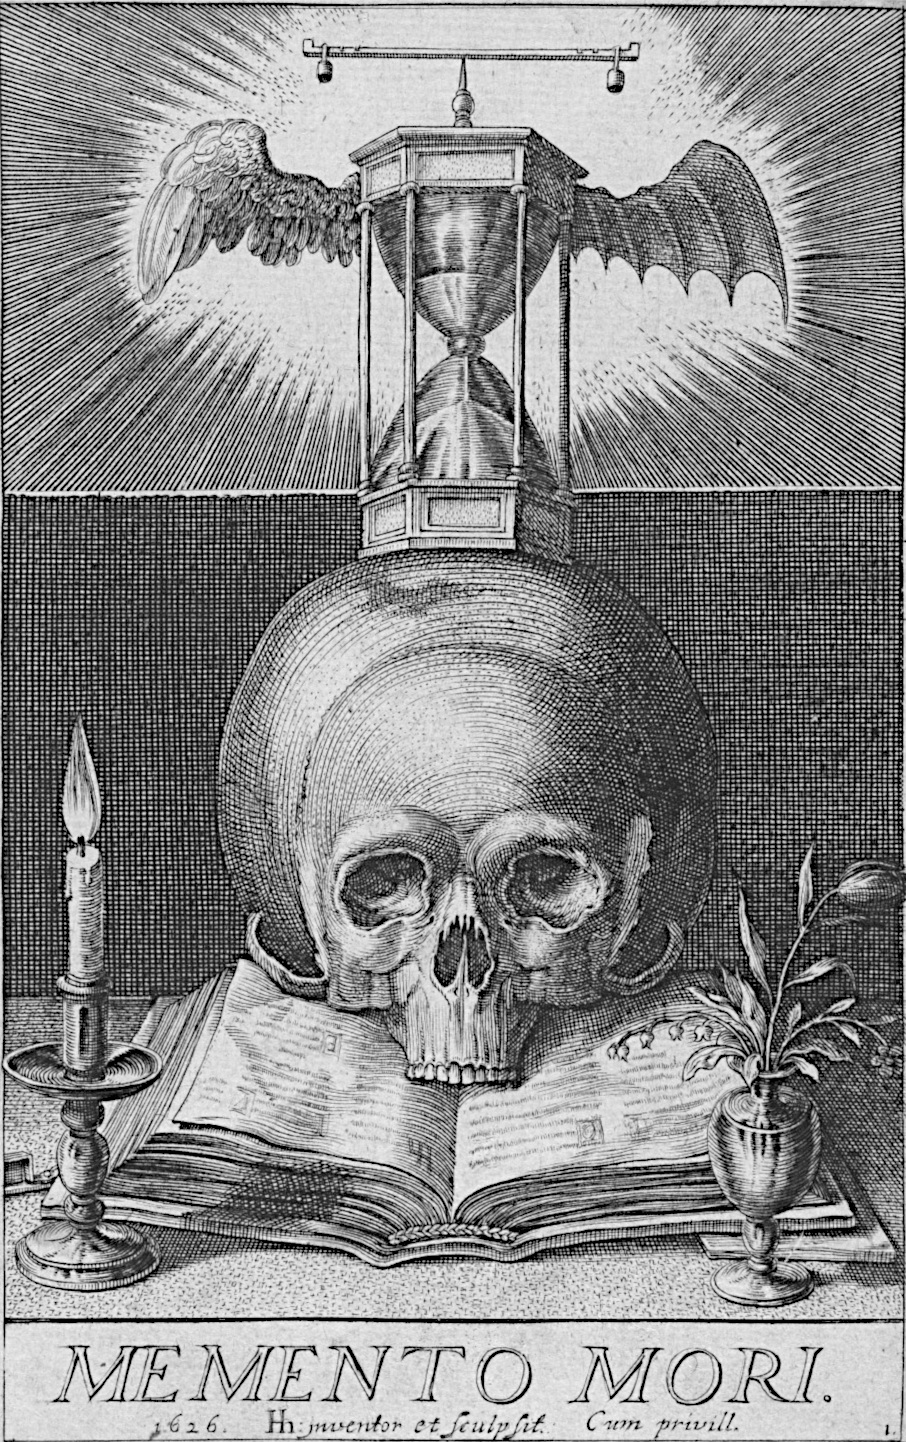
\includegraphics[keepaspectratio,width=\textwidth]{memento-mori-small.jpg}
  \captionart{MementoMori}
  \label{fig:mementomori}
\end{figure}

\clearpage{}
\thispagestyle{titleontop}
%SECT. II. MEMB. III. SUBSECT. V.-_Fear, a Cause_.
\section{Fear, a Cause.}

\lettrine{C}{ousin} german to sorrow, is fear, or rather a sister, fidus Achates,
and continual companion, an assistant and a principal agent in
procuring of this mischief; a cause and symptom as the other. In a
word, as \Virgil{}\authorfootnote{1657} of the Harpies, I may justly say of them both,
\li{Tristius haud illis monstrum, nec saevior ulla
Pestis et ira Deum stygiis sese extulit undis}.

A sadder monster, or more cruel plague so fell,
Or vengeance of the gods, ne'er came from Styx or Hell.

This foul fiend of fear was worshipped heretofore as a god by the
Lacedaemonians, and most of those other torturing \authorfootnote{1658}affections, and
so was sorrow amongst the rest, under the name of Angerona Dea, they
stood in such awe of them, as \Austin{}, de Civitat. Dei, lib. 4. cap. 8,
noteth out of Varro, fear was commonly \authorfootnote{1659}adored and painted in
their temples with a lion's head; and as Macrobius records, l. 10.
Saturnalium; \authorfootnote{1660}In the calends of January, Angerona had her holy
day, to whom in the temple of Volupia, or goddess of pleasure, their
augurs and bishops did yearly sacrifice; that, being propitious to
them, she might expel all cares, anguish, and vexation of the mind for
that year following. Many lamentable effects this fear causeth in men,
as to be red, pale, tremble, sweat, \authorfootnote{1661}it makes sudden cold and heat
to come over all the body, palpitation of the heart, syncope, \etc{}. It
amazeth many men that are to speak, or show themselves in public
assemblies, or before some great personages, as Tully confessed of
himself, that he trembled still at the beginning of his speech; and
Demosthenes, that great orator of Greece, before Philippus. It
confounds voice and memory, as Lucian wittily brings in Jupiter
Tragoedus, so much afraid of his auditory, when he was to make a speech
to the rest of the Gods, that he could not utter a ready word, but was
compelled to use Mercury's help in prompting. Many men are so amazed
and astonished with fear, they know not where they are, what they say,
\authorfootnote{1662}what they do, and that which is worst, it tortures them many days
before with continual affrights and suspicion. It hinders most
honourable attempts, and makes their hearts ache, sad and heavy. They
that live in fear are never free, \authorfootnote{1663}resolute, secure, never merry,
but in continual pain: that, as Vives truly said, Nulla est miseria
major quam metus, no greater misery, no rack, nor torture like unto it,
ever suspicious, anxious, solicitous, they are childishly drooping
without reason, without judgment, \authorfootnote{1664}especially if some terrible
object be offered, as Plutarch hath it. It causeth oftentimes sudden
madness, and almost all manner of diseases, as I have sufficiently
illustrated in my \authorfootnote{1665} digression of the force of imagination, and
shall do more at large in my section of \authorfootnote{1666}terrors. Fear makes our
imagination conceive what it list, invites the devil to come to us, as
\authorfootnote{1667}Agrippa and Cardan avouch, and tyranniseth over our phantasy more
than all other affections, especially in the dark. We see this verified
in most men, as Lavater saith\authorfootnote{1668}, Quae metuunt, fingunt; what they
fear they conceive, and feign unto themselves; they think they see
goblins, hags, devils, and many times become melancholy thereby.
Cardan, subtil. lib. 18, hath an example of such an one, so caused to
be melancholy (by sight of a bugbear) all his life after. Augustus
Caesar durst not sit in the dark, nisi aliquo assidente, saith
\authorfootnote{1669}Suetonius, Nunquam tenebris exigilavit. And 'tis strange what
women and children will conceive unto themselves, if they go over a
churchyard in the night, lie, or be alone in a dark room, how they
sweat and tremble on a sudden. Many men are troubled with future
events, foreknowledge of their fortunes, destinies, as Severus the
Emperor, Adrian and Domitian, Quod sciret ultimum vitae diem, saith
Suetonius, valde solicitus, much tortured in mind because he foreknew
his end; with many such, of which I shall speak more opportunely in
another place.\authorfootnote{1670} Anxiety, mercy, pity, indignation, \etc{}, and such
fearful branches derived from these two stems of fear and sorrow, I
voluntarily omit; read more of them in \authorfootnote{1671}Carolus Pascalius,
\authorfootnote{1672}Dandinus, \etc{}.

%SECT. II. MEMB. III. SUBSECT. VI.-_Shame and Disgrace, Causes_.
\section{Shame and Disgrace, Causes.}

\lettrine{S}{hame} and disgrace cause most violent passions and bitter pangs. Ob
pudorem et dedecus publicum, ob errorum commissum saepe moventur
generosi animi (Felix Plater, lib. 3. de alienat mentis.) Generous
minds are often moved with shame, to despair for some public disgrace.
And he, saith Philo, lib. 2. de provid. dei, \authorfootnote{1673}that subjects
himself to fear, grief, ambition, shame, is not happy, but altogether
miserable, tortured with continual labour, care, and misery. It is as
forcible a batterer as any of the rest: \authorfootnote{1674}Many men neglect the
tumults of the world, and care not for glory, and yet they are afraid
of infamy, repulse, disgrace (Tul. offic. l. 1), they can severely
contemn pleasure, bear grief indifferently, but they are quite
\authorfootnote{1675}battered and broken, with reproach and obloquy: (siquidem vita et
fama pari passu ambulant) and are so dejected many times for some
public injury, disgrace, as a box on the ear by their inferior, to be
overcome of their adversary, foiled in the field, to be out in a
speech, some foul fact committed or disclosed, \etc{} that they dare not
come abroad all their lives after, but melancholise in corners, and
keep in holes. The most generous spirits are most subject to it;
Spiritus altos frangit et generosos: Hieronymus. \Aristotle, because he
could not understand the motion of Euripus, for grief and shame drowned
himself: Caelius Rodigimus antiquar. lec. lib. 29. cap. 8. Homerus
pudore consumptus, was swallowed up with this passion of shame \authorfootnote{1676}
because he could not unfold the fisherman's riddle. Sophocles killed
himself, \authorfootnote{1677}for that a tragedy of his was hissed off the stage:
Valer. max. lib. 9. cap. 12. Lucretia stabbed herself, and so did
\authorfootnote{1678}Cleopatra, when she saw that she was reserved for a triumph, to
avoid the infamy. Antonius the Roman, \authorfootnote{1679}after he was overcome of
his enemy, for three days' space sat solitary in the fore-part of the
ship, abstaining from all company, even of Cleopatra herself, and
afterwards for very shame butchered himself, Plutarch, vita ejus.
Apollonius Rhodius \authorfootnote{1680}wilfully banished himself, forsaking his
country, and all his dear friends, because he was out in reciting his
poems, Plinius, lib. 7. cap. 23. Ajax ran mad, because his arms were
adjudged to Ulysses. In China 'tis an ordinary thing for such as are
excluded in those famous trials of theirs, or should take degrees, for
shame and grief to lose their wits, \authorfootnote{1681}Mat Riccius expedit. ad
Sinas, l. 3. c. 9. Hostratus the friar took that book which Reuclin had
writ against him, under the name of Epist. obscurorum virorum, so to
heart, that for shame and grief he made away with himself, \authorfootnote{1682}Jovius
in elogiis. A grave and learned minister, and an ordinary preacher at
Alcmar in Holland, was (one day as he walked in the fields for his
recreation) suddenly taken with a lax or looseness, and thereupon
compelled to retire to the next ditch; but being \authorfootnote{1683}surprised at
unawares, by some gentlewomen of his parish wandering that way, was so
abashed, that he did never after show his head in public, or come into
the pulpit, but pined away with melancholy: (Pet. Forestus med.
observat. lib. 10. observat. 12.) So shame amongst other passions can
play his prize.

I know there be many base, impudent, brazenfaced rogues, that will
\authorfootnote{1684} Nulla pallescere culpa, be moved with nothing, take no infamy or
disgrace to heart, laugh at all; let them be proved perjured,
stigmatised, convict rogues, thieves, traitors, lose their ears, be
whipped, branded, carted, pointed at, hissed, reviled, and derided with
\authorfootnote{1685}Ballio the Bawd in \Plautus{}, they rejoice at it, Cantores probos;
babe and Bombax, what care they? We have too many such in our times,
---\li{Exclamat Melicerta perisse}
---\li{Frontem de rebus.}\authormarginnote{1686}

Yet a modest man, one that hath grace, a generous spirit, tender of his
reputation, will be deeply wounded, and so grievously affected with it,
that he had rather give myriads of crowns, lose his life, than suffer
the least defamation of honour, or blot in his good name. And if so be
that he cannot avoid it, as a nightingale, \li{Que cantando victa moritur}
(saith Mizaldus\authorfootnote{1687}), dies for shame if another bird sing better, he
languisheth and pineth away in the anguish of his spirit.

\cleartoleftpage{}
\begin{figure}[p]
  \begingroup
  \centering
  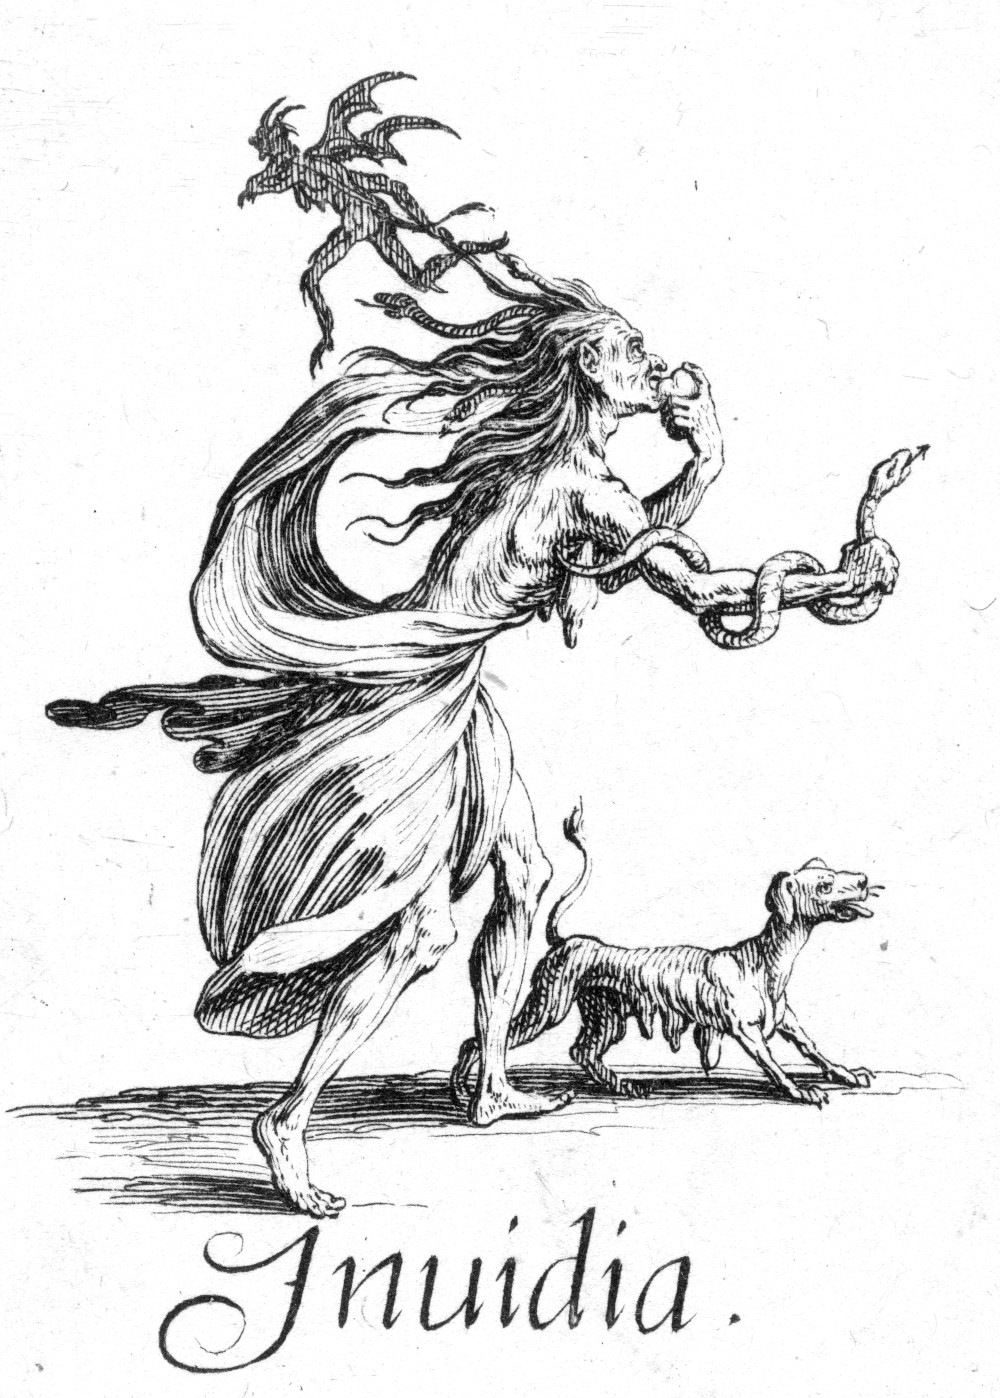
\includegraphics[keepaspectratio,width=0.9\textwidth]{nvidia-small.jpg}
  \captionart{Invidia}
  \label{fig:invidia}
\end{figure}

% Force float here
\clearpage{}
\thispagestyle{titleontop}

%SECT. II. MEMB. III. SUBSECT. VII.-_Envy, Malice, Hatred, Causes_.
\section{Envy, Malice, Hatred, Causes.}
\lettrine{E}{nvy} and malice are two links of this chain, and both, as Guianerius,
Tract. 15. cap. 2, proves out of Galen, 3 Aphorism, com. 22, \authorfootnote{1688}
cause this malady by themselves, especially if their bodies be
otherwise disposed to melancholy. 'Tis Valescus de Taranta, and Felix
Platerus' observation, \authorfootnote{1689}Envy so gnaws many men's hearts, that they
become altogether melancholy. And therefore belike Solomon, Prov. xiv.
13, calls it, the rotting of the bones, Cyprian, vulnus occultum;
\authorfootnote{1690}---Siculi non invenere tyranni
Majus tormentum---

The Sicilian tyrants never invented the like torment. It crucifies
their souls, withers their bodies, makes them hollow-eyed, \authorfootnote{1691}pale,
lean, and ghastly to behold, Cyprian, ser. 2. de zelo et livore.
\authorfootnote{1692}As a moth gnaws a garment, so, saith \Chrysostom{}, doth envy
consume a man; to be a living anatomy: a skeleton, to be a lean and
\authorfootnote{1693}pale carcass, quickened with a \authorfootnote{1694}fiend, Hall in Charact. for
so often as an envious wretch sees another man prosper, to be enriched,
to thrive, and be fortunate in the world, to get honours, offices, or
the like, he repines and grieves.

\begin{verse}
---\textlatin{intabescitque videndo\\*
  Successus hominum-suppliciumque suum est}\authorlatintrans{1695.5}.\authorfootnote{1695}
\end{verse}

He tortures himself if his equal, friend, neighbour, be preferred,
commended, do well; if he understand of it, it galls him afresh; and no
greater pain can come to him than to hear of another man's well-doing;
'tis a dagger at his heart every such object. He looks at him as they
that fell down in Lucian's rock of honour, with an envious eye, and
will damage himself, to do another a mischief: Atque cadet subito, dum
super hoste cadat. As he did in Aesop, lose one eye willingly, that his
fellow might lose both, or that rich man in \authorfootnote{1696}Quintilian that
poisoned the flowers in his garden, because his neighbour's bees should
get no more honey from them. His whole life is sorrow, and every word
he speaks a satire: nothing fats him but other men's ruins. For to
speak in a word, envy is nought else but Tristitia de bonis alienis,
sorrow for other men's good, be it present, past, or to come: et
gaudium de adversis, and \authorfootnote{1697}joy at their harms, opposite to mercy,
\authorfootnote{1698}which grieves at other men's mischances, and misaffects the body
in another kind; so Damascen defines it, lib. 2. de orthod. fid.
Thomas, 2. 2. quaest. 36. art. 1. \Aristotle, l. 2. Rhet. c. 4. et 10.
Plato Philebo. Tully, 3. Tusc. Greg. Nic. l. de virt. animae, c. 12.
Basil, de Invidia. Pindarus Od. 1. ser. 5, and we find it true. 'Tis a
common disease, and almost natural to us, as Tacitus holds\authorfootnote{1699}, to
envy another man's prosperity. And 'tis in most men an incurable
disease. \authorfootnote{1700}I have read, saith Marcus Aurelius, Greek, Hebrew,
Chaldee authors; I have consulted with many wise men for a remedy for
envy, I could find none, but to renounce all happiness, and to be a
wretch, and miserable for ever. 'Tis the beginning of hell in this
life, and a passion not to be excused. \authorfootnote{1701}Every other sin hath some
pleasure annexed to it, or will admit of an excuse; envy alone wants
both. Other sins last but for awhile; the gut may be satisfied, anger
remits, hatred hath an end, envy never ceaseth. Cardan, lib. 2. de sap.
Divine and humane examples are very familiar; you may run and read
them, as that of Saul and David, Cain and Abel, angebat illum non
proprium peccatum, sed fratris prosperitas, saith Theodoret, it was his
brother's good fortune galled him. Rachel envied her sister, being
barren, Gen. \rn{xxx.} Joseph's brethren him, Gen. \rn{xxxvii.} David had a touch
of this vice, as he confesseth, \authorfootnote{1702}Psal. 37. \authorfootnote{1703}Jeremy and
\authorfootnote{1704}Habakkuk, they repined at others' good, but in the end they
corrected themselves, Psal. 75, fret not thyself, \etc{}. Domitian spited
Agricola for his worth, \authorfootnote{1705}that a private man should be so much
glorified. \authorfootnote{1706}Cecinna was envied of his fellow-citizens, because he
was more richly adorned. But of all others, \authorfootnote{1707}women are most weak,
ob pulchritudinem invidae sunt foeminae (Musaeus) aut amat, aut odit,
nihil est tertium (Granatensis.) They love or hate, no medium amongst
them. Implacabiles plerumque laesae mulieres, Agrippina like, \authorfootnote{1708}A
woman, if she see her neighbour more neat or elegant, richer in tires,
jewels, or apparel, is enraged, and like a lioness sets upon her
husband, rails at her, scoffs at her, and cannot abide her; so the
Roman ladies in Tacitus did at Solonina, Cecinna's wife, \authorfootnote{1709}because
she had a better horse, and better furniture, as if she had hurt them
with it; they were much offended. In like sort our gentlewomen do at
their usual meetings, one repines or scoffs at another's bravery and
happiness. Myrsine, an Attic wench, was murdered of her fellows, \authorfootnote{1710}
because she did excel the rest in beauty, Constantine, Agricult. l. 11.
c. 7. Every village will yield such examples.

%SECT. II. MEMB. III. SUBSECT. VIII.-_Emulation, Hatred, Faction, Desire of Revenge, Causes_.
\section{Emulation, Hatred, Faction, Desire of Revenge, Causes.}

\lettrine{O}{ut} of this root of envy \authorfootnote{1711}spring those feral branches of faction,
hatred, livor, emulation, which cause the like grievances, and are,
serrae animae, the saws of the soul, \authorfootnote{1712}consternationis pleni
affectus, affections full of desperate amazement; or as Cyprian
describes emulation, it is \authorfootnote{1713}a moth of the soul, a consumption, to
make another man's happiness his misery, to torture, crucify, and
execute himself, to eat his own heart. Meat and drink can do such men
no good, they do always grieve, sigh, and groan, day and night without
intermission, their breast is torn asunder: and a little after,
\authorfootnote{1714}Whomsoever he is whom thou dost emulate and envy, he may avoid
thee, but thou canst neither avoid him nor thyself; wheresoever thou
art he is with thee, thine enemy is ever in thy breast, thy destruction
is within thee, thou art a captive, bound hand and foot, as long as
thou art malicious and envious, and canst not be comforted. It was the
devil's overthrow; and whensoever thou art thoroughly affected with
this passion, it will be thine. Yet no perturbation so frequent, no
passion so common.
%
\begin{verse}
\textgreek[variant=ancient]{Καὶ κεραμεὺς κεραμεῖ κοτέει\\
καὶ τεκτονι τέκτων},\\
\textgreek[variant=ancient]{Καὶ πτωχὸς πτωχῷ φθονέει\\
καὶ ἀοίδος ἀοιδῶ.}\authorfootnote{1715}
\end{verse}
\translationrule
\begin{verse}
A potter emulates a potter:\\
One smith envies another:\\

A beggar emulates a beggar;\\
A singing man his brother.\\
\end{verse}

Every society, corporation, and private family is full of it, it takes
hold almost of all sorts of men, from the prince to the ploughman, even
amongst gossips it is to be seen, scarce three in a company but there
is siding, faction, emulation, between two of them, some simultas, jar,
private grudge, heart-burning in the midst of them. Scarce two
gentlemen dwell together in the country, (if they be not near kin or
linked in marriage) but there is emulation betwixt them and their
servants, some quarrel or some grudge betwixt their wives or children,
friends and followers, some contention about wealth, gentry,
precedency, \etc{}, by means of which, like the frog in \authorfootnote{1716}Aesop, that
would swell till she was as big as an ox, burst herself at last; they
will stretch beyond their fortunes, callings, and strive so long that
they consume their substance in lawsuits, or otherwise in hospitality,
feasting, fine clothes, to get a few bombast titles, for ambitiosa
paupertate laboramus omnes, to outbrave one another, they will tire
their bodies, macerate their souls, and through contentions or mutual
invitations beggar themselves. Scarce two great scholars in an age, but
with bitter invectives they fall foul one on the other, and their
adherents; Scotists, Thomists, Reals, Nominals, Plato and \Aristotle,
Galenists and Paracelsians, \etc{}, it holds in all professions.
Honest \authorfootnote{1717}emulation in studies, in all callings is not to be
disliked, 'tis ingeniorum cos, as one calls it, the whetstone of wit,
the nurse of wit and valour, and those noble Romans out of this spirit
did brave exploits. There is a modest ambition, as Themistocles was
roused up with the glory of Miltiades; Achilles' trophies moved
Alexander,

\li{Ambire semper stulta confidentia est,
Ambire nunquam deses arrogantia est}\authorlatintrans{1718.5}.\authormarginnote{1718}

'Tis a sluggish humour not to emulate or to sue at all, to withdraw
himself, neglect, refrain from such places, honours, offices, through
sloth, niggardliness, fear, bashfulness, or otherwise, to which by his
birth, place, fortunes, education, he is called, apt, fit, and well
able to undergo; but when it is immoderate, it is a plague and a
miserable pain. What a deal of money did Henry \rn{VIII.} and Francis \rn{I.}
king of France, spend at that \authorfootnote{1719}famous interview? and how many vain
courtiers, seeking each to outbrave other, spent themselves, their
livelihood and fortunes, and died beggars? \authorfootnote{1720}Adrian the Emperor was
so galled with it, that he killed all his equals; so did Nero. This
passion made \authorfootnote{1721}Dionysius the tyrant banish Plato and Philoxenus the
poet, because they did excel and eclipse his glory, as he thought; the
Romans exile Coriolanus, confine Camillus, murder Scipio; the Greeks by
ostracism to expel Aristides, Nicias, Alcibiades, imprison Theseus,
make away Phocion, \etc{}. When Richard I. and Philip of France were fellow
soldiers together, at the siege of Acon in the Holy Land, and Richard
had approved himself to be the more valiant man, insomuch that all
men's eyes were upon him, it so galled Philip, Francum urebat Regis
victoria, saith mine \authorfootnote{1722}author, tam aegre ferebat Richardi gloriam,
ut carpere dicta, calumniari facta; that he cavilled at all his
proceedings, and fell at length to open defiance; he could contain no
longer, but hasting home, invaded his territories, and professed open
war. Hatred stirs up contention, Prov. x. 12, and they break out at
last into immortal enmity, into virulency, and more than Vatinian hate
and rage; \authorfootnote{1723}they persecute each other, their friends, followers,
and all their posterity, with bitter taunts, hostile wars, scurrile
invectives, libels, calumnies, fire, sword, and the like, and will not
be reconciled. Witness that Guelph and Ghibelline faction in Italy;
that of the Adurni and Fregosi in Genoa; that of Cneius Papirius, and
Quintus Fabius in Rome; Caesar and Pompey; Orleans and Burgundy in
France; York and Lancaster in England: yea, this passion so
rageth\authorfootnote{1724}many times, that it subverts not men only, and families,
but even populous cities. \authorfootnote{1725}Carthage and Corinth can witness as
much, nay, flourishing kingdoms are brought into a wilderness by it.
This hatred, malice, faction, and desire of revenge, invented first all
those racks and wheels, strappadoes, brazen bulls, feral engines,
prisons, inquisitions, severe laws to macerate and torment one another.
How happy might we be, and end our time with blessed days and sweet
content, if we could contain ourselves, and, as we ought to do, put up
injuries, learn humility, meekness, patience, forget and forgive, as in
\authorfootnote{1726}God's word we are enjoined, compose such final controversies
amongst ourselves, moderate our passions in this kind, and think better
of others, as Paul would have\authorfootnote{1727} us, than of ourselves: be of like
affection one towards another, and not avenge ourselves, but have peace
with all men. But being that we are so peevish and perverse, insolent
and proud, so factious and seditious, so malicious and envious; we do
invicem angariare, maul and vex one another, torture, disquiet, and
precipitate ourselves into that gulf of woes and cares, aggravate our
misery and melancholy, heap upon us hell and eternal damnation.

%SECT. II. MEMB. III. SUBSECT. IX.-_Anger, a Cause_.
\section{Anger, a Cause.}

\lettrine{A}{nger}, a perturbation, which carries the spirits outwards, preparing
the body to melancholy, and madness itself: Ira furor brevis est, anger
is temporary madness; and as Picolomineus accounts it\authorfootnote{1728}, one of the
three most violent passions. \authorfootnote{1729}Areteus sets it down for an especial
cause (so doth \Seneca, ep. 18. l. 1), of this malady. \authorfootnote{1730}Magninus
gives the reason, Ex frequenti ira supra modum calefiunt; it overheats
their bodies, and if it be too frequent, it breaks out into manifest
madness, saith St. Ambrose. 'Tis a known saying, Furor fit Iaesa
saepius palienlia, the most patient spirit that is, if he be often
provoked, will be incensed to madness; it will make a devil of a saint:
and therefore Basil (belike) in his Homily de Ira, calls it tenebras
rationis, morbum animae, et daemonem pessimum; the darkening of our
understanding, and a bad angel. \authorfootnote{1731}Lucian, in Abdicato, tom. 1, will
have this passion to work this effect, especially in old men and women.
Anger and calumny (saith he) trouble them at first, and after a while
break out into madness: many things cause fury in women, especially if
they love or hate overmuch, or envy, be much grieved or angry; these
things by little and little lead them on to this malady. From a
disposition they proceed to an habit, for there is no difference
between a mad man, and an angry man, in the time of his fit; anger, as
Lactantius describes it, L. de Ira Dei, ad Donatum, c. 5, is
\authorfootnote{1732}saeva animi tempestas, \etc{}, a cruel tempest of the mind; making
his eye sparkle fire, and stare, teeth gnash in his head, his tongue
stutter, his face pale, or red, and what more filthy imitation can be
of a mad man?
\authorfootnote{1733}Ora tument ira, fervescunt sanguine venae,
Lumina Gorgonio saevius angue micant.

They are void of reason, inexorable, blind, like beasts and monsters
for the time, say and do they know not what, curse, swear, rail, fight,
and what not? How can a mad man do more? as he said in the comedy,
\authorfootnote{1734} Iracundia non sum apud me, I am not mine own man. If these fits
be immoderate, continue long, or be frequent, without doubt they
provoke madness. Montanus, consil. 21, had a melancholy Jew to his
patient, he ascribes this for a principal cause: Irascebatur levibus de
causis, he was easily moved to anger. Ajax had no other beginning of
his madness; and Charles the Sixth, that lunatic French king, fell into
this misery, out of the extremity of his passion, desire of revenge and
malice, \authorfootnote{1735}incensed against the duke of Britain, he could neither
eat, drink, nor sleep for some days together, and in the end, about the
calends of July, 1392, he became mad upon his horseback, drawing his
sword, striking such as came near him promiscuously, and so continued
all the days of his life, Aemil., lib. 10. Gal. hist. Aegesippus de
exid. urbis Hieros, l. 1. c. 37, hath such a story of Herod, that out
of an angry fit, became mad, \authorfootnote{1736}leaping out of his bed, he killed
Jossippus, and played many such bedlam pranks, the whole court could
not rule him for a long time after: sometimes he was sorry and
repented, much grieved for that he had done, Postquam deferbuit ira, by
and by outrageous again. In hot choleric bodies, nothing so soon
causeth madness, as this passion of anger, besides many other diseases,
as Pelesius observes, cap. 21. l. 1. de hum. affect. causis; Sanguinem
imminuit, fel auget: and as Valesius controverts\authorfootnote{1737}, Med. controv.,
lib. 5. contro. 8, many times kills them quite out. If this were the
worst of this passion, it were more tolerable, \authorfootnote{1738}but it ruins and
subverts whole towns, \authorfootnote{1739}cities, families, and kingdoms; Nulla
pestis humano generi pluris stetit, saith \Seneca, de Ira, lib. 1. No
plague hath done mankind so much harm. Look into our histories, and you
shall almost meet with no other subject, but what a company \authorfootnote{1740}of
harebrains have done in their rage. We may do well therefore to put
this in our procession amongst the rest; From all blindness of heart,
from pride, vainglory, and hypocrisy, from envy, hatred and malice,
anger, and all such pestiferous perturbations, good Lord deliver us.

%SECT. II. MEMB. III. SUBSECT. X.-_Discontents, Cares, Miseries, \&c. Causes_.
\section{Discontents, Cares, Miseries, \&c. Causes.}

\lettrine{D}{iscontents}, cares, crosses, miseries, or whatsoever it is, that shall
cause any molestation of spirits, grief, anguish, and perplexity, may
well be reduced to this head (preposterously placed here in some men's
judgments they may seem), yet in that \Aristotle in his \authorfootnote{1741}Rhetoric
defines these cares, as he doth envy, emulation, \etc{} still by grief, I
think I may well rank them in this irascible row; being that they are
as the rest, both causes and symptoms of this disease, producing the
like inconveniences, and are most part accompanied with anguish and
pain. The common etymology will evince it, Cura quasi cor uro, Dementes
curae, insomnes curae, damnosae curae, tristes, mordaces, carnifices,
\etc{} biting, eating, gnawing, cruel, bitter, sick, sad, unquiet, pale,
tetric, miserable, intolerable cares, as the poets \authorfootnote{1742}call them,
worldly cares, and are as many in number as the sea sands. \authorfootnote{1743}Galen,
Fernelius, Felix Plater, Valescus de Taranta, \etc{}, reckon afflictions,
miseries, even all these contentions, and vexations of the mind, as
principal causes, in that they take away sleep, hinder concoction, dry
up the body, and consume the substance of it. They are not so many in
number, but their causes be as diverse, and not one of a thousand free
from them, or that can vindicate himself, whom that Ate dea,
\authorfootnote{1744}Per hominum capita molliter ambulans,
Plantas pedum teneras habens:

Over men's heads walking aloft,
With tender feet treading so soft,

Homer's Goddess Ate hath not involved into this discontented
\authorfootnote{1745}rank, or plagued with some misery or other. Hyginus, fab. 220, to
this purpose hath a pleasant tale. Dame Cura by chance went over a
brook, and taking up some of the dirty slime, made an image of it;
Jupiter eftsoons coming by, put life to it, but Cura and Jupiter could
not agree what name to give him, or who should own him; the matter was
referred to Saturn as judge; he gave this arbitrement: his name shall
be Homo ab humo, Cura eum possideat quamdiu vivat, Care shall have him
whilst he lives, Jupiter his soul, and Tellus his body when he dies.
But to leave tales. A general cause, a continuate cause, an inseparable
accident, to all men, is discontent, care, misery; were there no other
particular affliction (which who is free from?) to molest a man in this
life, the very cogitation of that common misery were enough to
macerate, and make him weary of his life; to think that he can never be
secure, but still in danger, sorrow, grief, and persecution. For to
begin at the hour of his birth, as \Pliny{} doth elegantly describe\authorfootnote{1746}
it, he is born naked, and falls \authorfootnote{1747}a whining at the very first: he
is swaddled, and bound up like a prisoner, cannot help himself, and so
he continues to his life's end. Cujusque ferae pabulum, saith
\authorfootnote{1748}\Seneca, impatient of heat and cold, impatient of labour,
impatient of idleness, exposed to fortune's contumelies. To a naked
mariner \Lucretius{} compares him, cast on shore by shipwreck, cold and
comfortless in an unknown land: \authorfootnote{1749}no estate, age, sex, can secure
himself from this common misery. A man that is born of a woman is of
short continuance, and full of trouble, Job \rn{xiv.} 1, 22. And while his
flesh is upon him he shall be sorrowful, and while his soul is in him
it shall mourn. All his days are sorrow and his travels griefs: his
heart also taketh not rest in the night. Eccles. \rn{ii.} 23, and \rn{ii.} 11.
All that is in it is sorrow and vexation of spirit. \authorfootnote{1750}Ingress,
progress, regress, egress, much alike: blindness seizeth on us in the
beginning, labour in the middle, grief in the end, error in all. What
day ariseth to us without some grief, care, or anguish? Or what so
secure and pleasing a morning have we seen, that hath not been overcast
before the evening? One is miserable, another ridiculous, a third
odious. One complains of this grievance, another of that. Aliquando
nervi, aliquando pedes vexant, (\Seneca) nunc distillatio, nunc epatis
morbus; nunc deest, nunc superest sanguis: now the head aches, then the
feet, now the lungs, then the liver, \etc{}. Huic sensus exuberat, sed est
pudori degener sanguis, \etc{}. He is rich, but base born; he is noble, but
poor; a third hath means, but he wants health peradventure, or wit to
manage his estate; children vex one, wife a second, \etc{}. Nemo facile cum
conditione sua concordat, no man is pleased with his fortune, a pound
of sorrow is familiarly mixed with a dram of content, little or no joy,
little comfort, but \authorfootnote{1751}everywhere danger, contention, anxiety, in
all places: go where thou wilt, and thou shalt find discontents, cares,
woes, complaints, sickness, diseases, encumbrances, exclamations: If
thou look into the market, there (saith \authorfootnote{1752} \Chrysostom{}) is brawling
and contention; if to the court, there knavery and flattery, \etc{}; if to
a private man's house, there's cark and care, heaviness, \etc{}. As he said
of old,
\authorfootnote{1753}Nil homine in terra spirat miserum magis alma?

No creature so miserable as man, so generally molested, \authorfootnote{1754}in
miseries of body, in miseries of mind, miseries of heart, in miseries
asleep, in miseries awake, in miseries wheresoever he turns, as Bernard
found, Nunquid tentatio est vita humana super terram? A mere temptation
is our life (\Austin{}, confess. lib. 10. cap. 28), \li{catena perpetuorum
malorum, et quis potest molestias et difficultates pati?} Who can endure
the miseries of it? \authorfootnote{1755}In prosperity we are insolent and
intolerable, dejected in adversity, in all fortunes foolish and
miserable. \authorfootnote{1756}In adversity I wish for prosperity, and in prosperity
I am afraid of adversity. What mediocrity may be found? Where is no
temptation? What condition of life is free? \authorfootnote{1757}Wisdom hath labour
annexed to it, glory, envy; riches and cares, children and
encumbrances, pleasure and diseases, rest and beggary, go together: as
if a man were therefore born (as the Platonists hold) to be punished in
this life for some precedent sins. Or that, as \Pliny{} complains\authorfootnote{1758},
Nature may be rather accounted a stepmother, than a mother unto us, all
things considered: no creature's life so brittle, so full of fear, so
mad, so furious; only man is plagued with envy, discontent, griefs,
covetousness, ambition, superstition. Our whole life is an Irish sea,
wherein there is nought to be expected but tempestuous storms and
troublesome waves, and those infinite,

\li{Tantum malorum pelagus aspicio,
Ut non sit inde enatandi copia}\authorlatintrans{1759.5},\authormarginnote{1759}

no halcyonian times, wherein a man can hold himself secure, or agree
with his present estate; but as Boethius infers, \authorfootnote{1760}there is
something in every one of us which before trial we seek, and having
tried abhor: \authorfootnote{1761} we earnestly wish, and eagerly covet, and are
eftsoons weary of it. Thus between hope and fear, suspicions, angers,
\authorfootnote{1762}Inter spemque metumque, timores inter et iras, betwixt falling
in, falling out, \etc{}, we bangle away our best days, befool out our
times, we lead a contentious, discontent, tumultuous, melancholy,
miserable life; insomuch, that if we could foretell what was to come,
and it put to our choice, we should rather refuse than accept of this
painful life. In a word, the world itself is a maze, a labyrinth of
errors, a desert, a wilderness, a den of thieves, cheaters, \etc{}, full
of filthy puddles, horrid rocks, precipitiums, an ocean of adversity,
an heavy yoke, wherein infirmities and calamities overtake, and follow
one another, as the sea waves; and if we scape Scylla, we fall foul on
Charybdis, and so in perpetual fear, labour, anguish, we run from one
plague, one mischief, one burden to another, duram servientes
servitutem, and you may as soon separate weight from lead, heat from
fire, moistness from water, brightness from the sun, as misery,
discontent, care, calamity, danger, from a man. Our towns and cities
are but so many dwellings of human misery. In which grief and sorrow
(\authorfootnote{1763}as he right well observes out of Solon) innumerable troubles,
labours of mortal men, and all manner of vices, are included, as in so
many pens. Our villages are like molehills, and men as so many emmets,
busy, busy still, going to and fro, in and out, and crossing one
another's projects, as the lines of several sea-cards cut each other in
a globe or map. Now light and merry, but (\authorfootnote{1764}as one follows it)
by-and-by sorrowful and heavy; now hoping, then distrusting; now
patient, tomorrow crying out; now pale, then red; running, sitting,
sweating, trembling, halting, \etc{}. Some few amongst the rest, or perhaps
one of a thousand, may be Pullus Jovis, in the world's esteem, Gallinae
filius albae, an happy and fortunate man, ad invidiam felix, because
rich, fair, well allied, in honour and office; yet peradventure ask
himself, and he will say, that of all others \authorfootnote{1765}he is most miserable
and unhappy. A fair shoe, Hic soccus novus, elegans, as he \authorfootnote{1766}said,
sed nescis ubi urat, but thou knowest not where it pincheth. It is not
another man's opinion can make me happy: but as \Seneca well hath\authorfootnote{1767}
it, He is a miserable wretch that doth not account himself happy,
though he be sovereign lord of a world: he is not happy, if he think
himself not to be so; for what availeth it what thine estate is, or
seem to others, if thou thyself dislike it? A common humour it is of
all men to think well of other men's fortunes, and dislike their own:
\authorfootnote{1768}Cui placet alterius, sua nimirum est odio sors; but \authorfootnote{1769}qui fit
Mecoenas, \etc{}, how comes it to pass, what's the cause of it? Many men
are of such a perverse nature, they are well pleased with nothing
(saith Theodoret\authorfootnote{1770}), neither with riches nor poverty, they
complain when they are well and when they are sick, grumble at all
fortunes, prosperity and adversity; they are troubled in a cheap year,
in a barren, plenty or not plenty, nothing pleaseth them, war nor
peace, with children, nor without. This for the most part is the humour
of us all, to be discontent, miserable, and most unhappy, as we think
at least; and show me him that is not so, or that ever was otherwise.
Quintus Metellus his felicity is infinitely admired amongst the Romans,
insomuch that as Paterculus mentioneth\authorfootnote{1771} of him, you can scarce
find of any nation, order, age, sex, one for happiness to be compared
unto him: he had, in a word, Bona animi, corporis et fortunae, goods of
mind, body, and fortune, so had P. Mutianus, \authorfootnote{1772}Crassus. Lampsaca,
that Lacedaemonian lady, was such another in \authorfootnote{1773}\Pliny{}'s conceit, a
king's wife, a king's mother, a king's daughter: and all the world
esteemed as much of Polycrates of Samos. The Greeks brag of their
Socrates, Phocion, Aristides; the Psophidians in particular of their
Aglaus, Omni vita felix, ab omni periculo immunis (which by the way
Pausanias held impossible;) the Romans of their \authorfootnote{1774} Cato, Curius,
Fabricius, for their composed fortunes, and retired estates, government
of passions, and contempt of the world: yet none of all these were
happy, or free from discontent, neither Metellus, Crassus, nor
Polycrates, for he died a violent death, and so did Cato; and how much
evil doth Lactantius and Theodoret speak of Socrates, a weak man, and
so of the rest. There is no content in this life, but as he said\authorfootnote{1775},
All is vanity and vexation of spirit; lame and imperfect. Hadst thou
Sampson's hair, Milo's strength, Scanderbeg's arm, Solomon's wisdom,
Absalom's beauty, Croesus' wealth, Pasetis obulum, Caesar's valour,
Alexander's spirit, Tully's or Demosthenes' eloquence, Gyges' ring,
Perseus' Pegasus, and Gorgon's head, Nestor's years to come, all this
would not make thee absolute; give thee content, and true happiness in
this life, or so continue it. Even in the midst of all our mirth,
jollity, and laughter, is sorrow and grief, or if there be true
happiness amongst us, 'tis but for a time,
\authorfootnote{1776}Desinat in piscem mulier formosa superne:

A handsome woman with a fish's tail, a fair morning turns to a lowering afternoon. Brutus and Cassius, once
renowned, both eminently happy, yet you shall scarce find two (saith
Paterculus) quos fortuna maturius destiturit, whom fortune sooner
forsook. Hannibal, a conqueror all his life, met with his match, and
was subdued at last, Occurrit forti, qui mage fortis erit. One is
brought in triumph, as Caesar into Rome, Alcibiades into Athens,
coronis aureis donatus, crowned, honoured, admired; by-and-by his
statues demolished, he hissed out, massacred, \etc{}. \authorfootnote{1777}Magnus
Gonsalva, that famous Spaniard, was of the prince and people at first
honoured, approved; forthwith confined and banished. Admirandas
actiones; graves plerunque sequuntur invidiae, et acres calumniae: 'tis
Polybius his observation, grievous enmities, and bitter calumnies,
commonly follow renowned actions. One is born rich, dies a beggar;
sound today, sick tomorrow; now in most flourishing estate, fortunate
and happy, by-and-by deprived of his goods by foreign enemies, robbed
by thieves, spoiled, captivated, impoverished, as they of \authorfootnote{1778}Rabbah
put under iron saws, and under iron harrows, and under axes of iron,
and cast into the tile kiln,

\begin{verse}
\textlatin{Quid me felicem toties jactastis amici},\\
\textlatin{Qui cecidit, stabili non erat ille gradu.}\authorfootnote{1779}
\end{verse}

He that erst marched like Xerxes with innumerable armies, as rich as
Croesus, now shifts for himself in a poor cock-boat, is bound in iron
chains, with Bajazet the Turk, and a footstool with Aurelian, for a
tyrannising conqueror to trample on. So many casualties there are, that
as \Seneca said of a city consumed with fire, Una dies interest inter
maximum civitatem et nullam, one day betwixt a great city and none: so
many grievances from outward accidents, and from ourselves, our own
indiscretion, inordinate appetite, one day betwixt a man and no man.
And which is worse, as if discontents and miseries would not come fast
enough upon us: homo homini daemon, we maul, persecute, and study how
to sting, gall, and vex one another with mutual hatred, abuses,
injuries; preying upon and devouring as so many, \authorfootnote{1780}ravenous birds;
and as jugglers, panders, bawds, cozening one another; or raging as
\authorfootnote{1781}wolves, tigers, and devils, we take a delight to torment one
another; men are evil, wicked, malicious, treacherous, and
\authorfootnote{1782}naught, not loving one another, or loving themselves, not
hospitable, charitable, nor sociable as they ought to be, but
counterfeit, dissemblers, ambidexters, all for their own ends,
hard-hearted, merciless, pitiless, and to benefit themselves, they care
not what mischief they procure to others. \authorfootnote{1783}Praxinoe and Gorgo in
the poet, when they had got in to see those costly sights, they then
cried bene est, and would thrust out all the rest: when they are rich
themselves, in honour, preferred, full, and have even that they would,
they debar others of those pleasures which youth requires, and they
formerly have enjoyed. He sits at table in a soft chair at ease, but he
doth remember in the mean time that a tired waiter stands behind him,
an hungry fellow ministers to him full, he is athirst that gives him
drink (saith \authorfootnote{1784}Epictetus) and is silent whilst he speaks his
pleasure: pensive, sad, when he laughs. Pleno se proluit auro: he
feasts, revels, and profusely spends, hath variety of robes, sweet
music, ease, and all the pleasure the world can afford, whilst many an
hunger-starved poor creature pines in the street, wants clothes to
cover him, labours hard all day long, runs, rides for a trifle, fights
peradventure from sun to sun, sick and ill, weary, full of pain and
grief, is in great distress and sorrow of heart. He loathes and scorns
his inferior, hates or emulates his equal, envies his superior, insults
over all such as are under him, as if he were of another species, a
demigod, not subject to any fall, or human infirmities. Generally they
love not, are not beloved again: they tire out others' bodies with
continual labour, they themselves living at ease, caring for none else,
sibi nati; and are so far many times from putting to their helping
hand, that they seek all means to depress, even most worthy and well
deserving, better than themselves, those whom they are by the laws of
nature bound to relieve and help, as much as in them lies, they will
let them caterwaul, starve, beg, and hang, before they will any ways
(though it be in their power) assist or ease: \authorfootnote{1785}so unnatural are
they for the most part, so unregardful; so hard-hearted, so churlish,
proud, insolent, so dogged, of so bad a disposition. And being so
brutish, so devilishly bent one towards another, how is it possible but
that we should be discontent of all sides, full of cares, woes, and
miseries?

If this be not a sufficient proof of their discontent and misery,
examine every condition and calling apart. Kings, princes, monarchs,
and magistrates seem to be most happy, but look into their estate, you
shall \authorfootnote{1786}find them to be most encumbered with cares, in perpetual
fear, agony, suspicion, jealousy: that, as he said\authorfootnote{1787} of a crown, if
they knew but the discontents that accompany it, they would not stoop
to take it up. Quem mihi regent dabis (saith \Chrysostom{}) non curis
plenum? What king canst thou show me, not full of cares? \authorfootnote{1788}Look not
on his crown, but consider his afflictions; attend not his number of
servants, but multitude of crosses. Nihil aliud potestas culminis, quam
tempestas mentis, as Gregory seconds him; sovereignty is a tempest of
the soul: Sylla like they have brave titles, but terrible fits:
splendorem titulo, cruciatum animo: which made \authormarginnote{1789}Demosthenes vow,
si vel ad tribunal, vel ad interitum duceretur: if to be a judge, or to
be condemned, were put to his choice, he would be condemned. Rich men
are in the same predicament; what their pains are, stulti nesciunt,
ipsi sentiunt: they feel, fools perceive not, as I shall prove
elsewhere, and their wealth is brittle, like children's rattles: they
come and go, there is no certainty in them: those whom they elevate,
they do as suddenly depress, and leave in a vale of misery. The middle
sort of men are as so many asses to bear burdens; or if they be free,
and live at ease, they spend themselves, and consume their bodies and
fortunes with luxury and riot, contention, emulation, \etc{}. The poor I
reserve for another \authorfootnote{1790}place and their discontents.
For particular professions, I hold as of the rest, there's no content
or security in any; on what course will you pitch, how resolve? to be a
divine, 'tis contemptible in the world's esteem; to be a lawyer, 'tis
to be a wrangler; to be a physician, \authorfootnote{1791}pudet lotii, 'tis loathed; a
philosopher, a madman; an alchemist, a beggar; a poet, esurit, an
hungry jack; a musician, a player; a schoolmaster, a drudge; an
husbandman, an emmet; a merchant, his gains are uncertain; a
mechanician, base; a chirurgeon, fulsome; a tradesman, a \authorfootnote{1792}liar; a
tailor, a thief; a serving-man, a slave; a soldier, a butcher; a smith,
or a metalman, the pot's never from his nose; a courtier a parasite, as
he could find no tree in the wood to hang himself; I can show no state
of life to give content. The like you may say of all ages; children
live in a perpetual slavery, still under that tyrannical government of
masters; young men, and of riper years, subject to labour, and a
thousand cares of the world, to treachery, falsehood, and cozenage,
%
\begin{verse}
---\textlatin{Incedit per ignes},\\
\textlatin{Suppositos cineri doloso},\authorfootnote{1793}
\end{verse}
\translationrule
\begin{verse}
---you incautious tread\\
On fires, with faithless ashes overhead.
\end{verse}

\authorfootnote{1794}old are full of aches in their bones, cramps and convulsions,
silicernia, dull of hearing, weak sighted, hoary, wrinkled, harsh, so
much altered as that they cannot know their own face in a glass, a
burthen to themselves and others, after 70 years, all is sorrow (as
David hath it), they do not live but linger. If they be sound, they
fear diseases; if sick, weary of their lives: Non est vivere, sed
valere vita. One complains of want, a second of servitude,
\authorfootnote{1795}another of a secret or incurable disease; of some deformity of
body, of some loss, danger, death of friends, shipwreck, persecution,
imprisonment, disgrace, repulse, \authorfootnote{1796} contumely, calumny, abuse,
injury, contempt, ingratitude, unkindness, scoffs, flouts, unfortunate
marriage, single life, too many children, no children, false servants,
unhappy children, barrenness, banishment, oppression, frustrate hopes
and ill-success, \etc{}.
%
\begin{verse}
\textlatin{Talia de genere hoc adeo sunt multa, loquacem ut}\\
\textlatin{Delassare valent Fabium}.---\authorfootnote{1797}
\end{verse}
\translationrule
\begin{verse}
But, every various instance to repeat,\\
Would tire even Fabius of incessant prate.
\end{verse}

Talking Fabius will be tired before he can tell half of them; they are
the subject of whole volumes, and shall (some of them) be more
opportunely dilated elsewhere. In the meantime thus much I may say of
them, that generally they crucify the soul of man, \authorfootnote{1798}attenuate our
bodies, dry them, wither them, shrivel them up like old apples, make
them as so many anatomies (\authorfootnote{1799}ossa atque pellis est totus, ita curis
macet) they cause tempus foedum et squalidum, cumbersome days,
ingrataque tempora, slow, dull, and heavy times: make us howl, roar,
and tear our hairs, as sorrow did in \authorfootnote{1800}Cebes' table, and groan for
the very anguish of our souls. Our hearts fail us as David's did, Psal.
\rn{xl.} 12, for innumerable troubles that compassed him; and we are ready
to confess with Hezekiah, Isaiah \rn{lviii.} 17, behold, for felicity I had
bitter grief; to weep with Heraclitus, to curse the day of our birth
with Jeremy, \rn{xx.} 14, and our stars with Job: to hold that axiom of
Silenus, \authorfootnote{1801}better never to have been born, and the best next of
all, to die quickly: or if we must live, to abandon the world, as Timon
did; creep into caves and holes, as our anchorites; cast all into the
sea, as Crates Thebanus; or as Theombrotus Ambrociato's 400 auditors,
precipitate ourselves to be rid of these miseries.

%SECT. II. MEMB. III. SUBSECT. XI.-_Concupiscible Appetite, as Desires, Ambition, Causes_.
\section{Concupiscible Appetite, as Desires, Ambition, Causes.}

\lettrine{T}{hese} \footnoteA{worthy of being desired. \theeditor{}}{concupiscible} and \footnoteA{irritable. \theeditor{}}{irascible} appetites are as the two twists of a
rope, mutually mixed one with the other, and both twining about the
heart: both good, as \Austin{}, holds, l. 14. c. 9. de civ. Dei, \authorfootnote{1802}if
they be moderate; both pernicious if they be exorbitant. This
concupiscible appetite, howsoever it may seem to carry with it a show
of pleasure and delight, and our concupiscences most part affect us
with content and a pleasing object, yet if they be in extremes, they
rack and wring us on the other side. A true saying it is, Desire hath
no rest; is infinite in itself, endless; and as one calls\authorfootnote{1803} it, a
perpetual rack, \authorfootnote{1804}or horse-mill, according to \Austin{}, still going
round as in a ring. They are not so continual, as diverse, \li{felicius
atomos denumerare possem}, saith Bernard\authorfootnote{1805}, \li{quam motus cordis; nunc
haec, nunc illa cogito}, you may as well reckon up the motes in the sun
as them. It extends itself to everything\authorfootnote{1806}, as Guianerius will have
it, that is superfluously sought after:' or to any \authorfootnote{1807}fervent
desire, as Fernelius interprets it; be it in what kind soever, it
tortures if immoderate, and is (according to Plater\authorfootnote{1808} and others)
an especial cause of melancholy. \li{Multuosis concupiscentiis dilaniantur
cogitationes meae}, \Austin{} confessed\authorfootnote{1809}, that he was torn a pieces
with his manifold desires: and so doth Bernard complain\authorfootnote{1810}, that he
could not rest for them a minute of an hour: this I would have, and
that, and then I desire to be such and such. 'Tis a hard matter
therefore to confine them, being they are so various and many,
impossible to apprehend all. I will only insist upon some few of the
chief, and most noxious in their kind, as that exorbitant appetite and
desire of honour, which we commonly call ambition; love of money, which
is covetousness, and that greedy desire of gain: self-love, pride, and
inordinate desire of vainglory or applause, love of study in excess;
love of women (which will require a just volume of itself), of the
other I will briefly speak, and in their order.

Ambition, a proud covetousness, or a dry thirst of honour, a great
torture of the mind, composed of envy, pride, and covetousness, a
gallant madness, one defines\authorfootnote{1811} it a pleasant poison, Ambrose, a
canker of the soul, an hidden plague: Bernard\authorfootnote{1812}, a secret poison,
the father of livor, and mother of hypocrisy, the moth of holiness, and
cause of madness, crucifying and disquieting all that it takes hold of.
\Seneca calls it\authorfootnote{1813}, \li{rem solicitam, timidam, vanam, ventosam}, a windy
thing, a vain, solicitous, and fearful thing. For commonly they that,
like Sisyphus, roll this restless stone of ambition, are in a perpetual
agony, still perplexed\authorfootnote{1814}, \li{semper taciti, tritesque recedunt}
(\Lucretius{}), doubtful, timorous, suspicious, loath to offend in word or
deed, still cogging and colloguing, embracing, capping, cringing,
applauding, flattering, fleering, visiting, waiting at men's doors,
with all affability, counterfeit honesty and humility. If that
will not serve\authorfootnote{1815}, if once this humour (as Cyprian describes\authorfootnote{1816} it)
possess his thirsty soul, ambitionis salsugo ubi bibulam animam
possidet, by hook and by crook he will obtain it, and from his hole he
will climb to all honours and offices, if it be possible for him to get
up, flattering one, bribing another, he will leave no means unessay'd
to win all. It is a wonder to see how slavishly these kind of men
subject themselves\authorfootnote{1817}, when they are about a suit, to every inferior
person; what pains they will take, run, ride, cast, plot, countermine,
protest and swear, vow, promise, what labours undergo, early up, down
late; how obsequious and affable they are, how popular and courteous,
how they grin and fleer upon every man they meet; with what feasting
and inviting, how they spend themselves and their fortunes, in seeking
that many times, which they had much better be without; as Cyneas
the orator told\authorfootnote{1818} Pyrrhus: with what waking nights, painful hours,
anxious thoughts, and bitterness of mind, \li{inter spemque metumque},
distracted and tired, they consume the interim of their time. There can
be no greater plague for the present. If they do obtain their suit,
which with such cost and solicitude they have sought, they are not so
freed, their anxiety is anew to begin, for they are never satisfied,
\li{nihil aliud nisi imperium spirant}, their thoughts, actions, endeavours
are all for sovereignty and honour, like Lues Sforza\authorfootnote{1819} that huffing
Duke of Milan, a man of singular wisdom, but profound ambition, born to
his own, and to the destruction of Italy, though it be to their own
ruin, and friends' undoing, they will contend, they may not cease, but
as a dog in a wheel, a bird in a cage, or a squirrel in a chain, so
Budaeus compares\authorfootnote{1820} them; they climb and climb still\authorfootnote{1821}, with
much labour, but never make an end, never at the top. A knight would be
a baronet, and then a lord, and then a viscount, and then an earl, \etc{};
a doctor, a dean, and then a bishop; from tribune to praetor; from
bailiff to major; first this office, and then that; as Pyrrhus in
Plutarch\authorfootnote{1822}, they will first have Greece, then Africa, and then
Asia, and swell with Aesop's frog so long, till in the end they burst,
or come down with Sejanus, ad Gemonias scalas, and break their own
necks; or as Evangelus the piper in Lucian, that blew his pipe so long,
till he fell down dead. If he chance to miss, and have a canvass, he is
in a hell on the other side; so dejected, that he is ready to hang
himself, turn heretic, Turk, or traitor in an instant. Enraged against
his enemies, he rails, swears, fights, slanders, detracts, envies,
murders: and for his own part, si appetitum explere non potest, furore
corripitur; if he cannot satisfy his desire (as Bodine writes\authorfootnote{1823}) he
runs mad. So that both ways, hit or miss, he is distracted so long as
his ambition lasts, he can look for no other but anxiety and care,
discontent and grief in the meantime, madness itself\authorfootnote{1824}, or violent
death in the end. The event of this is common to be seen in populous
cities, or in princes' courts, for a courtier's life (as Budaeus
describes it) is a \footnoteA{a hodgepodge; jumble; confused medley. \theeditor{}}{gallimaufry} of ambition\authorfootnote{1825}, lust, fraud,
imposture, dissimulation, detraction, envy, pride; \authorfootnote{1826}the court, a
common conventicle of flatterers, time-servers, politicians, \etc{}; or as
\authorfootnote{1827} Anthony Perez will, the suburbs of hell itself. If you will see
such discontented persons, there you shall likely find them. And
which he observed of the markets of old Rome\authorfootnote{1828},
%
\begin{latin}
\begin{quote}
Qui perjurum convenire vult hominem, mitto in Comitium;
Qui mendacem et gloriosum, apud Cluasinae sacrum;
Dites, damnosos maritos, sub basilica quaerito, \etc{}.
\end{quote}
\end{latin}
\translationrule
\begin{quote}
Perjured knaves, knights of the post, liars, crackers, bad husbands,
\etc{} keep their several stations; they do still, and always did in every
commonwealth.
\end{quote}

%SECT. II. MEMB. III. SUBSECT. XII.-_Φιλαργυρία, Covetousness, a Cause_.
\section{\textgreek{Φιλαργυρία}, Covetousness, a Cause.}

\lettrine{P}{lutarch}, in his book\authorfootnote{1829} whether the diseases of the body be more
grievous than those of the soul, is of opinion, if you will examine all
the causes of our miseries in this life, you shall find them most part
to have had their beginning from stubborn anger, that furious desire of
contention, or some unjust or immoderate affection, as covetousness,
\etc{}. From whence are wars and contentions amongst you? \authorfootnote{1830}St. James
asks: I will add usury, fraud, rapine, simony, oppression, lying,
swearing, bearing false witness, \etc{} are they not from this fountain of
covetousness, that greediness in getting, tenacity in keeping,
sordidity in spending; that they are so wicked, \authorfootnote{1831}unjust against
God, their neighbour, themselves; all comes hence. The desire of money
is the root of all evil, and they that lust after it, pierce themselves
through with many sorrows, 1 Tim. vi. 10. Hippocrates therefore in his
Epistle to Crateva, an herbalist, gives him this good counsel, that if
it were possible, \authorfootnote{1832} amongst other herbs, he should cut up that
weed of covetousness by the roots, that there be no remainder left, and
then know this for a certainty, that together with their bodies, thou
mayst quickly cure all the diseases of their minds. For it is indeed
the pattern, image, epitome of all melancholy, the fountain of many
miseries, much discontented care and woe; this inordinate, or
immoderate desire of gain, to get or keep money, as Bonaventure
defines\authorfootnote{1833} it: or, as \Austin{} describes it, a madness of the soul, Gregory
a torture; \Chrysostom{}, an insatiable drunkenness; Cyprian, blindness,
speciosum supplicium, a plague subverting kingdoms, families, an
\authorfootnote{1834}incurable disease; Budaeus, an ill habit, \authorfootnote{1835}yielding to no
remedies: neither Aesculapius nor Plutus can cure them: a continual
plague, saith Solomon, and vexation of spirit, another hell. I know
there be some of opinion, that covetous men are happy, and worldly,
wise, that there is more pleasure in getting of wealth than in
spending, and no delight in the world like unto it. 'Twas Bias'
problem\authorfootnote{1836} of old, With what art thou not weary? with getting money. What
is most delectable? to gain. What is it, trow you, that makes a poor
man labour all his lifetime, carry such great burdens, fare so hardly,
macerate himself, and endure so much misery, undergo such base offices
with so great patience, to rise up early, and lie down late, if there
were not an extraordinary delight in getting and keeping of money? What
makes a merchant that hath no need, satis superque domi, to range all
over the world, through all those intemperate \authorfootnote{1837}Zones of heat and
cold; voluntarily to venture his life, and be content with such
miserable famine, nasty usage, in a stinking ship; if there were not a
pleasure and hope to get money, which doth season the rest, and
mitigate his indefatigable pains? What makes them go into the bowels of
the earth, an hundred fathom deep, endangering their dearest lives,
enduring damps and filthy smells, when they have enough already, if
they could be content, and no such cause to labour, but an
extraordinary delight they take in riches. This may seem plausible at
first show, a popular and strong argument; but let him that so thinks,
consider better of it, and he shall soon perceive, that it is far
otherwise than he supposeth; it may be haply pleasing at the first, as
most part all melancholy is. For such men likely have some lucida
intervalla, pleasant symptoms intermixed; but you must note that of
\authorfootnote{1838}\Chrysostom{}, 'Tis one thing to be rich, another to be covetous:
generally they are all fools, dizzards, madmen, \authorfootnote{1839}miserable
wretches, living besides themselves, sine arte fruendi, in perpetual
slavery, fear, suspicion, sorrow, and discontent, plus aloes quam
mellis habent; and are indeed, rather possessed by their money, than
possessors: as Cyprian hath\authorfootnote{1840} it, \li{mancipati pecuniis}; bound
prentice to their goods, as \Pliny{}\authorfootnote{1841}; or as \Chrysostom{}, servi
divitiarum, slaves and drudges to their substance; and we may conclude
of them all, as Valerius doth\authorfootnote{1842} of Ptolomaeus king of Cyprus, He
was in title a king of that island, but in his mind, a miserable drudge
of money:
\authorfootnote{1843}---potiore metallis
libertate carens---

wanting his liberty, which is better than gold. Damasippus the Stoic,
in \Horace{}, proves that all mortal men dote by fits, some one way, some
another, but that covetous men \authorfootnote{1844}are madder than the rest; and he
that shall truly look into their estates, and examine their symptoms,
shall find no better of them, but that they are all \authorfootnote{1845}fools, as
Nabal was, Re et nomine (1. Reg. 15.) For what greater folly can there
be, or \authorfootnote{1846} madness, than to macerate himself when he need not? and
when, as Cyprian notes, \authorfootnote{1847}he may be freed from his burden, and
eased of his pains, will go on still, his wealth increasing, when he
hath enough, to get more, to live besides himself, to starve his
genius, keep back from his wife \authorfootnote{1848}and children, neither letting
them nor other friends use or enjoy that which is theirs by right, and
which they much need perhaps; like a hog, or dog in the manger, he doth
only keep it, because it shall do nobody else good, hurting himself and
others: and for a little momentary pelf, damn his own soul? They are
commonly sad and tetric by nature, as Achab's spirit was because he
could not get Naboth's vineyard, (1. Reg. 22.) and if he lay out his
money at any time, though it be to necessary uses, to his own
children's good, he brawls and scolds, his heart is heavy, much
disquieted he is, and loath to part from it: \li{Miser abstinet et timet
uti}.\authorfootnote{1848.8} He is of a wearish, dry, pale constitution, and cannot sleep
for cares and worldly business; his riches, saith Solomon, will not let
him sleep, and unnecessary business which he heapeth on himself; or if
he do sleep, 'tis a very unquiet, interrupt, unpleasing sleep: with his
bags in his arms,
---congestis undique sacc
indormit inhians,---

And though he be at a banquet, or at some merry feast, he sighs for
grief of heart (as Cyprian hath\authorfootnote{1849} it) and cannot sleep though it be
upon a down bed; his wearish body takes no rest, \authorfootnote{1850}troubled in his
abundance, and sorrowful in plenty, unhappy for the present, and more
unhappy in the life to come. Basil. He is a perpetual drudge,
\authorfootnote{1851}restless in his thoughts, and never satisfied, a slave, a wretch,
a dust-worm, semper quod idolo suo immolet, sedulus observat Cypr.
prolog. ad sermon still seeking what sacrifice he may offer to his
golden god, per fas et nefas, he cares not how, his trouble is endless,
\authorfootnote{1852}crescunt divitiae, tamen curtae nescio quid semper abest rei: his
wealth increaseth, and the more he hath, the more \authorfootnote{1853}he wants: like
Pharaoh's lean kine, which devoured the fat, and were not satisfied.
\authorfootnote{1854}\Austin{} therefore defines covetousness, quarumlibet rerum
inhonestam et insatiabilem cupiditatem a dishonest and insatiable
desire of gain; and in one of his epistles compares it to hell;
\authorfootnote{1855}which devours all, and yet never hath enough, a bottomless pit,
an endless misery; in quem scopulum avaritiae cadaverosi senes
utplurimum impingunt, and that which is their greatest corrosive, they
are in continual suspicion, fear, and distrust, He thinks his own wife
and children are so many thieves, and go about to cozen him, his
servants are all false:
%
\begin{verse}
\textlatin{Rem suam periisse, seque eradicarier},\\
\textlatin{Et divum atque hominum clamat continuo fidem},\\
\textlatin{De suo tigillo si qua exit foras}.
\end{verse}
\translationrule
\begin{verse}
If his doors creek, then out he cries anon,\\
His goods are gone, and he is quite undone.
\end{verse}

Timidus Plutus, an old proverb, As fearful as Plutus: so doth
Aristophanes and Lucian bring him in fearful still, pale, anxious,
suspicious, and trusting no man, \authorfootnote{1856}They are afraid of tempests for
their corn; they are afraid of their friends lest they should ask
something of them, beg or borrow; they are afraid of their enemies lest
they hurt them, thieves lest they rob them; they are afraid of war and
afraid of peace, afraid of rich and afraid of poor; afraid of all. Last
of all, they are afraid of want, that they shall die beggars, which
makes them lay up still, and dare not use that they have: what if a
dear year come, or dearth, or some loss? and were it not that they are
both to \authorfootnote{1857}lay out money on a rope, they would be hanged forthwith,
and sometimes die to save charges, and make away themselves, if their
corn and cattle miscarry; though they have abundance left, as
\authorfootnote{1858}Agellius notes. \authorfootnote{1859}Valerius makes mention of one that in a
famine sold a mouse for 200 pence, and famished himself: such are their
cares, \authorfootnote{1860}griefs and perpetual fears. These symptoms are elegantly
expressed by Theophrastus in his character of a covetous man;
\authorfootnote{1861}lying in bed, he asked his wife whether she shut the trunks and
chests fast, the cap-case be sealed, and whether the hall door be
bolted; and though she say all is well, he riseth out of his bed in his
shirt, barefoot and barelegged, to see whether it be so, with a dark
lantern searching every corner, scarce sleeping a wink all night.
Lucian in that pleasant and witty dialogue called Gallus, brings in
Mycillus the cobbler disputing with his cock, sometimes Pythagoras;
where after much speech pro and con, to prove the happiness of a mean
estate, and discontents of a rich man, Pythagoras' cock in the end, to
illustrate by examples that which he had said, brings him to Gnyphon
the usurer's house at midnight, and after that to Encrates; whom, they
found both awake, casting up their accounts, and telling of their
money, \authorfootnote{1862}lean, dry, pale and anxious, still suspecting lest
somebody should make a hole through the wall, and so get in; or if a
rat or mouse did but stir, starting upon a sudden, and running to the
door to see whether all were fast. \Plautus{}, in his Aulularia, makes old
Euclio \authorfootnote{1863}commanding Staphyla his wife to shut the doors fast, and
the fire to be put out, lest anybody should make that an errand to come
to his house: when he washed his hands, \authorfootnote{1864}he was loath to fling
away the foul water, complaining that he was undone, because the smoke
got out of his roof. And as he went from home, seeing a crow scratch
upon the muck-hill, returned in all haste, taking it for malum omen, an
ill sign, his money was digged up; with many such. He that will but
observe their actions, shall find these and many such passages not
feigned for sport, but really performed, verified indeed by such
covetous and miserable wretches, and that it is,
\authorfootnote{1865}---manifesta phrenesis
Ut locuples moriaris egenti vivere fato.

A mere madness, to live like a wretch, and die rich.

%SECT. II. MEMB. III. SUBSECT. XIII.-_Love of Gaming, \etc{} and pleasures immoderate; Causes_.
\section[Love of Gaming]{Love of Gaming, \etc{} and pleasures immoderate; Causes.}

\lettrine{I}{t} is a wonder to see, how many poor, distressed, miserable wretches,
one shall meet almost in every path and street, begging for an alms,
that have been well descended, and sometimes in flourishing estate, now
ragged, tattered, and ready to be starved, lingering out a painful
life, in discontent and grief of body and mind, and all through
immoderate lust, gaming, pleasure and riot. 'Tis the common end of all
sensual epicures and brutish prodigals, that are stupefied and carried
away headlong with their several pleasures and lusts. Cebes in his
table, St. Ambrose in his second book of Abel and Cain, and amongst the
rest Lucian in his tract de Mercede conductis, hath excellent well
deciphered such men's proceedings in his picture of Opulentia, whom he
feigns to dwell on the top of a high mount, much sought after by many
suitors; at their first coming they are generally entertained by
pleasure and dalliance, and have all the content that possibly may be
given, so long as their money lasts: but when their means fail, they
are contemptibly thrust out at a back door, headlong, and there left to
shame, reproach, despair. And he at first that had so many attendants,
parasites, and followers, young and lusty, richly arrayed, and all the
dainty fare that might be had, with all kind of welcome and good
respect, is now upon a sudden stripped of all, \authorfootnote{1866}pale, naked, old,
diseased and forsaken, cursing his stars, and ready to strangle
himself; having no other company but repentance, sorrow, grief,
derision, beggary, and contempt, which are his daily attendants to his
life's end. As the \authorfootnote{1867}prodigal son had exquisite music, merry
company, dainty fare at first; but a sorrowful reckoning in the end; so
have all such vain delights and their followers. \authorfootnote{1868}Tristes
voluptatum exitus, et quisquis voluptatum suarum reminisci volet,
intelliget, as bitter as gall and wormwood is their last; grief of
mind, madness itself. The ordinary rocks upon which such men do impinge
and precipitate themselves, are cards, dice, hawks, and hounds, Insanum
venandi studium, one calls it, insanae substructiones: their mad
structures, disports, plays, \etc{}, when they are unseasonably used,
imprudently handled, and beyond their fortunes. Some men are consumed
by mad fantastical buildings, by making galleries, cloisters, terraces,
walks, orchards, gardens, pools, rillets, bowers, and such like places
of pleasure; Inutiles domos, \authorfootnote{1869}Xenophon calls them, which howsoever
they be delightsome things in themselves, and acceptable to all
beholders, an ornament, and benefiting some great men: yet unprofitable
to others, and the sole overthrow of their estates. Forestus in his
observations hath an example of such a one that became melancholy upon
the like occasion, having consumed his substance in an unprofitable
building, which would afterward yield him no advantage. Others, I say,
are \authorfootnote{1870} overthrown by those mad sports of hawking and hunting;
honest recreations, and fit for some great men, but not for every base
inferior person; whilst they will maintain their falconers, dogs, and
hunting nags, their wealth, saith \authorfootnote{1871}Salmutze, runs away with
hounds, and their fortunes fly away with hawks. They persecute beasts
so long, till in the end they themselves degenerate into beasts, as
\authorfootnote{1872}Agrippa taxeth them, \authorfootnote{1873}Actaeon like, for as he was eaten to
death by his own dogs, so do they devour themselves and their
patrimonies, in such idle and unnecessary disports, neglecting in the
mean time their more necessary business, and to follow their vocations.
Over-mad too sometimes are our great men in delighting, and doting too
much on it. \authorfootnote{1874}When they drive poor husbandmen from their tillage,
as Sarisburiensis objects\authorfootnote{1875}, Polycrat. l. 1. c. 4, fling down
country farms, and whole towns, to make parks, and forests, starving
men to feed beasts, and \authorfootnote{1876}punishing in the mean time such a man
that shall molest their game, more severely than him that is otherwise
a common hacker, or a notorious thief. But great men are some ways to
be excused, the meaner sort have no evasion why they should not be
counted mad. Poggius the Florentine tells a merry story to this
purpose, condemning the folly and impertinent business of such kind of
persons. A physician of Milan, saith he, that cured mad men, had a pit
of water in his house, in which he kept his patients, some up to the
knees, some to the girdle, some to the chin, pro modo insaniae, as they
were more or less affected. One of them by chance, that was well
recovered, stood in the door, and seeing a gallant ride by with a hawk
on his fist, well mounted, with his spaniels after him, would needs
know to what use all this preparation served; he made answer to kill
certain fowls; the patient demanded again, what his fowl might be worth
which he killed in a year; he replied 5 or 10 crowns; and when he urged
him farther what his dogs, horse, and hawks stood him in, he told him
400 crowns; with that the patient bad be gone, as he loved his life and
welfare, for if our master come and find thee here, he will put thee in
the pit amongst mad men up to the chin: taxing the madness and folly of
such vain men that spend themselves in those idle sports, neglecting
their business and necessary affairs. Leo Decimus, that hunting pope,
is much discommended by \authorfootnote{1877}Jovius in his life, for his immoderate
desire of hawking and hunting, in so much that (as he saith) he would
sometimes live about Ostia weeks and months together, leave suitors
\authorfootnote{1878}unrespected, bulls and pardons unsigned, to his own prejudice,
and many private men's loss. \authorfootnote{1879}And if he had been by chance crossed
in his sport, or his game not so good, he was so impatient, that he
would revile and miscall many times men of great worth with most bitter
taunts, look so sour, be so angry and waspish, so grieved and molested,
that it is incredible to relate it. But if he had good sport, and been
well pleased, on the other side, incredibili munificentia, with
unspeakable bounty and munificence he would reward all his fellow
hunters, and deny nothing to any suitor when he was in that mood. To
say truth, 'tis the common humour of all gamesters, as Galataeus
observes, if they win, no men living are so jovial and merry, but
\authorfootnote{1880}if they lose, though it be but a trifle, two or three games at
tables, or a dealing at cards for two pence a game, they are so
choleric and testy that no man may speak with them, and break many
times into violent passions, oaths, imprecations, and unbeseeming
speeches, little differing from mad men for the time. Generally of all
gamesters and gaming, if it be excessive, thus much we may conclude,
that whether they win or lose for the present, their winnings are not
Munera fortunae, sed insidiae as that wise \Seneca determines, not
fortune's gifts, but baits, the common catastrophe is \authorfootnote{1881}beggary,
\authorfootnote{1882}Ut pestis vitam, sic adimit alea pecuniam, as the plague takes
away life, doth gaming goods, for \authorfootnote{1883} omnes nudi, inopes et egeni;
\authorfootnote{1884}Alea Scylla vorax, species certissima furti,
Non contenta bonis animum quoque perfida mergit,
Foeda, furax, infamis, iners, furiosa, ruina.

For a little pleasure they take, and some small gains and gettings now
and then, their wives and children are ringed in the meantime, and they
themselves with loss of body and soul rue it in the end. I will say
nothing of those prodigious prodigals, perdendae pecuniae, genitos, as
he \authorfootnote{1885} taxed Anthony, Qui patrimonium sine ulla fori calumnia
amittunt, saith \authorfootnote{1886}Cyprian, and \authorfootnote{1887}mad sybaritical spendthrifts,
Quique una comedunt patrimonia coena; that eat up all at a breakfast,
at a supper, or amongst bawds, parasites, and players, consume
themselves in an instant, as if they had flung it into \authorfootnote{1888}Tiber,
with great wages, vain and idle expenses, \etc{}, not themselves only, but
even all their friends, as a man desperately swimming drowns him that
comes to help him, by suretyship and borrowing they will willingly undo
all their associates and allies. \authorfootnote{1889} Irati pecuniis, as he saith,
angry with their money: \authorfootnote{1890}what with a wanton eye, a liquorish
tongue, and a gamesome hand, when they have indiscreetly impoverished
themselves, mortgaged their wits, together with their lands, and
entombed their ancestors' fair possessions in their bowels, they may
lead the rest of their days in prison, as many times they do; they
repent at leisure; and when all is gone begin to be thrifty: but Sera
est in fundo parsimonia, 'tis then too late to look about; their
\authorfootnote{1891}end is misery, sorrow, shame, and discontent. And well they
deserve to be infamous and discontent. \authorfootnote{1892}Catamidiari in
Amphitheatro, as by Adrian the emperor's edict they were of old,
decoctores bonorum suorum, so he calls them, prodigal fools, to be
publicly shamed, and hissed out of all societies, rather than to be
pitied or relieved. \authorfootnote{1893}The Tuscans and Boetians brought their
bankrupts into the marketplace in a bier with an empty purse carried
before them, all the boys following, where they sat all day
circumstante plebe, to be infamous and ridiculous. At \authorfootnote{1894}Padua in
Italy they have a stone called the stone of turpitude, near the
senate-house, where spendthrifts, and such as disclaim non-payment of
debts, do sit with their hinder parts bare, that by that note of
disgrace others may be terrified from all such vain expense, or
borrowing more than they can tell how to pay. The \authorfootnote{1895}civilians of
old set guardians over such brain-sick prodigals, as they did over
madmen, to moderate their expenses, that they should not so loosely
consume their fortunes, to the utter undoing of their families.
I may not here omit those two main plagues, and common dotages of human
kind, wine and women, which have infatuated and besotted myriads of
people; they go commonly together.

\li{Qui vino indulget, quemque aloa decoquit, ille
In venerem putret}\authorlatintrans{1896.5}---\authormarginnote{1896}

To whom is sorrow, saith Solomon, Pro. \rn{xxiii.} 39, to whom is woe, but
to such a one as loves drink? it causeth torture, (vino tortus et ira)
and bitterness of mind, Sirac. 31. 21. Vinum furoris, Jeremy calls it,
15. cap. wine of madness, as well he may, for insanire facit sanos, it
makes sound men sick and sad, and wise men \authorfootnote{1897}mad, to say and do
they know not what. Accidit hodie terribilis casus (saith \authorfootnote{1898}S.
\Austin{}) hear a miserable accident; Cyrillus' son this day in his drink,
Matrem praegnantem nequiter oppressit, sororem violare voluit, patrem
occidit fere, et duas alias sorores ad mortem vulneravit, would have
violated his sister, killed his father, \etc{}. A true saying it was of
him, Vino dari laetitiam et dolorem, drink causeth mirth, and drink
causeth sorrow, drink causeth poverty and want, (Prov. \rn{xxi.}) shame and
disgrace. Multi ignobiles evasere ob vini potum, et (\Austin{}) amissis
honoribus profugi aberrarunt: many men have made shipwreck of their
fortunes, and go like rogues and beggars, having turned all their
substance into aurum potabile, that otherwise might have lived in good
worship and happy estate, and for a few hours' pleasure, for their
Hilary term's but short, or \authorfootnote{1899}free madness, as \Seneca calls it,
purchase unto themselves eternal tediousness and trouble.
That other madness is on women, Apostatare facit cor, saith the wise
man, \authorfootnote{1900}Atque homini cerebrum minuit. Pleasant at first she is, like
Dioscorides Rhododaphne, that fair plant to the eye, but poison to the
taste, the rest as bitter as wormwood in the end (Prov. \rn{v.} 4.) and
sharp as a two-edged sword, (\rn{vii.} 27.) Her house is the way to hell,
and goes down to the chambers of death. What more sorrowful can be
said? they are miserable in this life, mad, beasts, led like \authorfootnote{1901}oxen
to the slaughter: and that which is worse, whoremasters and drunkards
shall be judged, amittunt gratiam, saith \Austin{}, perdunt gloriam,
incurrunt damnationem aeternam. They lose grace and glory;
\authorfootnote{1902}---brevis illa voluptas
Abrogat aeternum caeli decus---

they gain hell and eternal damnation.

%SECT. II. MEMB. III. SUBSECT. XIV.-_Philautia, or Self-love, Vainglory, Praise, Honour, Immoderate Applause, Pride, overmuch Joy, \etc{}, Causes_.
\section[\textgreek{Φιλαυτία}, or Self-love]{\textgreek{Φιλαυτία}, or Self-love, Vainglory, Praise, Honour, Immoderate Applause, Pride, overmuch Joy, \etc{}, Causes.}
\lettrine{S}{elf-love}, pride, and vainglory, \authorfootnote{1903}caecus amor sui, which
\Chrysostom{} calls one of the devil's three great nets; \authorfootnote{1904}Bernard, an
arrow which pierceth the soul through, and slays it; a sly, insensible
enemy, not perceived, are main causes. Where neither anger, lust,
covetousness, fear, sorrow, \etc{}, nor any other perturbation can lay
hold; this will slyly and insensibly pervert us, Quem non gula vicit,
Philautia, superavit, (saith Cyprian) whom surfeiting could not
overtake, self-love hath overcome. \authorfootnote{1905}He hath scorned all money,
bribes, gifts, upright otherwise and sincere, hath inserted himself to
no fond imagination, and sustained all those tyrannical concupiscences
of the body, hath lost all his honour, captivated by vainglory.
\Chrysostom{}, sup. Io. Tu sola animum mentemque peruris, gloria. A great
assault and cause of our present malady, although we do most part
neglect, take no notice of it, yet this is a violent batterer of our
souls, causeth melancholy and dotage. This pleasing humour; this soft
and whispering popular air, Amabilis insania; this delectable frenzy,
most irrefragable passion, Mentis gratissimus error, this acceptable
disease, which so sweetly sets upon us, ravisheth our senses, lulls our
souls asleep, puffs up our hearts as so many bladders, and that without
all feeling, \authorfootnote{1906}insomuch as those that are misaffected with it,
never so much as once perceive it, or think of any cure. We commonly
love him best in this \authorfootnote{1907}malady, that doth us most harm, and are
very willing to be hurt; adulationibus nostris libentur facemus (saith
\authorfootnote{1908} Jerome) we love him, we love him for it: \authorfootnote{1909}O Bonciari suave,
suave fuit a te tali haec tribui; 'Twas sweet to hear it. And as
\authorfootnote{1910}\Pliny{} doth ingenuously confess to his dear friend Augurinus, all
thy writings are most acceptable, but those especially that speak of
us. Again, a little after to Maximus, \authorfootnote{1911}I cannot express how
pleasing it is to me to hear myself commended. Though we smile to
ourselves, at least ironically, when parasites bedaub us with false
encomiums, as many princes cannot choose but do, Quum tale quid nihil
intra se repererint, when they know they come as far short, as a mouse
to an elephant, of any such virtues; yet it doth us good. Though we
seem many times to be angry, \authorfootnote{1912} and blush at our own praises, yet
our souls inwardly rejoice, it puffs us up; 'tis fallax suavitas,
blandus daemon, makes us swell beyond our bounds, and forget ourselves.
Her two daughters are lightness of mind, immoderate joy and pride, not
excluding those other concomitant vices, which \authorfootnote{1913}Iodocus Lorichius
reckons up; bragging, hypocrisy, peevishness, and curiosity.
Now the common cause of this mischief, ariseth from ourselves or
others, \authorfootnote{1914}we are active and passive. It proceeds inwardly from
ourselves, as we are active causes, from an overweening conceit we have
of our good parts, own worth, (which indeed is no worth) our bounty,
favour, grace, valour, strength, wealth, patience, meekness,
hospitality, beauty, temperance, gentry, knowledge, wit, science, art,
learning, our \authorfootnote{1915} excellent gifts and fortunes, for which,
Narcissus-like, we admire, flatter, and applaud ourselves, and think
all the world esteems so of us; and as deformed women easily believe
those that tell them they be fair, we are too credulous of our own good
parts and praises, too well persuaded of ourselves. We brag and
venditate our \authorfootnote{1916}own works, and scorn all others in respect of us;
Inflati scientia, (saith Paul) our wisdom, \authorfootnote{1917}our learning, all our
geese are swans, and we as basely esteem and vilify other men's, as we
do over-highly prize and value our own. We will not suffer them to be
in secundis, no, not in tertiis; what, Mecum confertur Ulysses? they
are Mures, Muscae, culices prae se, nits and flies compared to his
inexorable and supercilious, eminent and arrogant worship: though
indeed they be far before him. Only wise, only rich, only fortunate,
valorous, and fair, puffed up with this tympany of self-conceit;
\authorfootnote{1918}as that proud Pharisee, they are not (as they suppose) like other
men, of a purer and more precious metal: \authorfootnote{1919}Soli rei gerendi sunt
efficaces, which that wise Periander held of such: \authorfootnote{1920}meditantur
omne qui prius negotium, \etc{}. Novi quendam (saith \authorfootnote{1921}Erasmus) I knew
one so arrogant that he thought himself inferior to no man living, like
\authorfootnote{1922}Callisthenes the philosopher, that neither held Alexander's acts,
or any other subject worthy of his pen, such was his insolency; or
Seleucus king of Syria, who thought none fit to contend with him but
the Romans. \authorfootnote{1923}Eos solos dignos ratus quibuscum de imperio certaret.
That which Tully writ to Atticus long since, is still in force.
\authorfootnote{1924}There was never yet true poet nor orator, that thought any other
better than himself. And such for the most part are your princes,
potentates, great philosophers, historiographers, authors of sects or
heresies, and all our great scholars, as Hierom defines\authorfootnote{1925}; a
natural philosopher is a glorious creature, and a very slave of rumour,
fame, and popular opinion, and though they write de contemptu gloriae,
yet as he observes, they will put their names to their books. Vobis et
famae, me semper dedi, saith Trebellius Pollio, I have wholly
consecrated myself to you and fame. 'Tis all my desire, night and day,
'tis all my study to raise my name. Proud \authorfootnote{1926}\Pliny{} seconds him;
Quamquam O! \etc{} and that vainglorious \authorfootnote{1927}orator is not ashamed to
confess in an Epistle of his to Marcus Lecceius, Ardeo incredibili
cupididate, \etc{}. I burn with an incredible desire to have my \authorfootnote{1928}name
registered in thy book. Out of this fountain proceed all those cracks
and brags,-\authorfootnote{1929}speramus carmina fingi Posse linenda cedro, et leni
servanda cupresso-\authorfootnote{1930}Non usitata nec tenui ferar penna.-nec in terra
morabor longius. Nil parvum aut humili modo, nil mortale loquor. Dicar
qua violens obstrepit Ausidus.-Exegi monumentum aere perennius. Iamque
opus exegi, quod nec Jovis ira, nec ignis, \etc{} cum venit ille dies, \etc{}
parte tamen meliore mei super alta perennis astra ferar, nomenque erit
indelebile nostrum. (This of \Ovid I have paraphrased in English.)

\begin{verse}
And when I am dead and gone,\\
My corpse laid under a stone\\
My fame shall yet survive,\\
And I shall be alive,\\
In these my works for ever,\\
My glory shall persever, \etc{}
\end{verse}

And that of Ennius,
%
\settowidth{\versewidth}{Nemo me lachrymis decoret, neque funera fletu}
\textlatin{\begin{verse}
Nemo me lachrymis decoret,\\
neque funera fletu\\
Faxit, cur?\\
volito docta per ora virum.
\end{verse}}
\translationrule
\settowidth{\versewidth}{Let none shed tears over me, or adorn my bier with sorrow}
\begin{verse}
Let none shed tears over me,\\
or adorn my bier with sorrow\\
because I am eternally in the mouths of men.
\end{verse}

With many such proud strains, and foolish flashes too common with writers. Not so much as Democharis on
the \authorfootnote{1931} Topics, but he will be immortal. Typotius de fama, shall be
famous, and well he deserves, because he writ of fame; and every
trivial poet must be renowned,-Plausuque petit clarescere vulgi. He
seeks the applause of the public. This puffing humour it is, that hath
produced so many great tomes, built such famous monuments, strong
castles, and Mausolean tombs, to have their acts eternised,-Digito
monstrari, et dicier hic est; to be pointed at with the finger, and to
have it said 'there he goes,' to see their names inscribed, as Phryne
on the walls of Thebes, Phryne fecit; this causeth so many bloody
battles,-Et noctes cogit vigilare serenas; and induces us to watch
during calm nights. Long journeys, Magnum iter intendo, sed dat mihi
gloria vires, I contemplate a monstrous journey, but the love of glory
strengthens me for it, gaining honour, a little applause, pride,
self-love, vainglory. This is it which makes them take such pains, and
break out into those ridiculous strains, this high conceit of
themselves, to \authorfootnote{1932}scorn all others; ridiculo fastu et intolerando
contemptu; as Palaemon the grammarian contemned\authorfootnote{1933} Varro, secum et
natas et morituras literas jactans, and brings them to that height of
insolency, that they cannot endure to be contradicted, \authorfootnote{1934}or hear of
anything but their own commendation, which Hierom notes of such kind of
men. And as \Austin{} well seconds\authorfootnote{1935} him, 'tis their sole study day
and night to be commended and applauded. When as indeed, in all wise
men's judgments, \li{quibus cor sapit}, they are \authorfootnote{1936}mad, empty vessels,
funges, beside themselves, derided, \li{et ut Camelus in proverbio quaerens
cornua, etiam quas habebat aures amisit}\authorlatintrans{1937}, their works are toys, as
an almanac out of date, \authorfootnote{1938}\li{authoris pereunt garrulitate sui}, they
seek fame and immortality, but reap dishonour and infamy, they are a
common obloquy, insensati, and come far short of that which they
suppose or expect. \authorfootnote{1939}\li{O puer ut sis vitalis metuo},
---How much I dread
Thy days are short, some lord shall strike thee dead.

Of so many myriads of poets, rhetoricians, philosophers, sophisters, as
\authorfootnote{1940}Eusebius well observes, which have written in former ages, scarce
one of a thousand's works remains, nomina et libri simul cum corporibus
interierunt, their books and bodies are perished together. It is not as
they vainly think, they shall surely be admired and immortal, as one
told Philip of Macedon insultingly, after a victory, that his shadow
was no longer than before, we may say to them,
%
\begin{verse}
\textlatin{Nos demiramur, sed non cum deside vulgo,}\\
\textlatin{Sed velut Harpyas, Gorgonas, et Furias.}
\end{verse}
\translationrule
\begin{verse}
We marvel too, not as the vulgar we,\\
But as we Gorgons, Harpies, or Furies see.
\end{verse}

Or if we do applaud, honour and admire, quota pars, how small a part,
in respect of the whole world, never so much as hears our names, how
few take notice of us, how slender a tract, as scant as Alcibiades'
land in a map! And yet every man must and will be immortal, as he
hopes, and extend his fame to our antipodes, when as half, no not a
quarter of his own province or city, neither knows nor hears of him-but
say they did, what's a city to a kingdom, a kingdom to Europe, Europe
to the world, the world itself that must have an end, if compared to
the least visible star in the firmament, eighteen times bigger than it?
and then if those stars be infinite, and every star there be a sun, as
some will, and as this sun of ours hath his planets about him, all
inhabited, what proportion bear we to them, and where's our glory?
Orbem terrarum victor Romanus habebat, as he cracked in Petronius, all
the world was under Augustus: and so in Constantine's time, Eusebius
brags he governed all the world, universum mundum praeclare admodum
administravit,-et omnes orbis gentes Imperatori subjecti: so of
Alexander it is given out, the four monarchies, \etc{} when as neither
Greeks nor Romans ever had the fifteenth part of the now known world,
nor half of that which was then described. What braggadocios are they
and we then? quam brevis hic de nobis sermo, as he said\authorfootnote{1941},
\authorfootnote{1942}pudebit aucti nominis, how short a time, how little a while doth
this fame of ours continue? Every private province, every small
territory and city, when we have all done, will yield as generous
spirits, as brave examples in all respects, as famous as ourselves,
Cadwallader in Wales, Rollo in Normandy, Robin Hood and Little John,
are as much renowned in Sherwood, as Caesar in Rome, Alexander in
Greece, or his Hephestion, \authorfootnote{1943} Omnis aetas omnisque populus in
exemplum et admirationem veniet, every town, city, book, is full of
brave soldiers, senators, scholars; and though \authorfootnote{1944}Bracyclas was a
worthy captain, a good man, and as they thought, not to be matched in
Lacedaemon, yet as his mother truly said, plures habet Sparta Bracyda
meliores, Sparta had many better men than ever he was; and howsoever
thou admirest thyself, thy friend, many an obscure fellow the world
never took notice of, had he been in place or action, would have done
much better than he or he, or thou thyself.
Another kind of mad men there is opposite to these, that are insensibly
mad, and know not of it, such as contemn all praise and glory, think
themselves most free, when as indeed they are most mad: calcant sed
alio fastu: a company of cynics, such as are monks, hermits,
anchorites, that contemn the world, contemn themselves, contemn all
titles, honours, offices: and yet in that contempt are more proud than
any man living whatsoever. They are proud in humility, proud in that
they are not proud, saepe homo de vanae gloriae contemptu, vanius
gloriatur, as \Austin{} hath it, confess. lib. 10, cap. 38, like Diogenes,
intus gloriantur, they brag inwardly, and feed themselves fat with a
self-conceit of sanctity, which is no better than hypocrisy. They go in
sheep's russet, many great men that might maintain themselves in cloth
of gold, and seem to be dejected, humble by their outward carriage,
when as inwardly they are swollen full of pride, arrogancy, and
self-conceit. And therefore \Seneca adviseth his friend Lucilius,
\authorfootnote{1945}in his attire and gesture, outward actions, especially to avoid
all such things as are more notable in themselves: as a rugged attire,
hirsute head, horrid beard, contempt of money, coarse lodging, and
whatsoever leads to fame that opposite way.

All this madness yet proceeds from ourselves, the main engine which
batters us is from others, we are merely passive in this business: from
a company of parasites and flatterers, that with immoderate praise, and
bombast epithets, glossing titles, false eulogiums, so bedaub and
applaud, gild over many a silly and undeserving man, that they clap him
quite out of his wits. Res imprimis violenta est, as Hierom notes, this
common applause is a most violent thing, laudum placenta, a drum, fife,
and trumpet cannot so animate; that fattens men, erects and dejects
them in an instant. \authorfootnote{1946} Palma negata macrum, donata reducit opimum.
It makes them fat and lean, as frost doth conies. \authorfootnote{1947}And who is that
mortal man that can so contain himself, that if he be immoderately
commended and applauded, will not be moved? Let him be what he will,
those parasites will overturn him: if he be a king, he is one of the
nine worthies, more than a man, a god forthwith,-\authorfootnote{1948}edictum Domini
Deique nostri: and they will sacrifice unto him,

---\li{divinos si tu patiaris honores,
Ultro ipsi dabimus meritasque sacrabimus aras}\authorlatintrans{1949.5}.\authormarginnote{1949}

If he be a soldier, then Themistocles, Epaminondas, Hector, Achilles,
duo fulmina belli, triumviri terrarum, \etc{}, and the valour of both
Scipios is too little for him, he is invictissimus, serenissimus,
multis trophaeus ornatissimus, naturae, dominus, although he be lepus
galeatus, indeed a very coward, a milk-sop, \authorfootnote{1950}and as he said of
Xerxes, postremus in pugna, primus in fuga, and such a one as never
durst look his enemy in the face. If he be a big man, then is he a
Samson, another Hercules; if he pronounce a speech, another Tully or
Demosthenes; as of Herod in the Acts, the voice of God and not of man:
if he can make a verse, Homer, \Virgil{}, \etc{}, And then my silly weak
patient takes all these eulogiums to himself; if he be a scholar so
commended for his much reading, excellent style, method, \etc{}, he will
eviscerate himself like a spider, study to death, Laudatas ostendit
avis Junonia pennas, peacock-like he will display all his feathers. If
he be a soldier, and so applauded, his valour extolled, though it be
impar congressus, as that of Troilus and Achilles, Infelix puer, he
will combat with a giant, run first upon a breach, as another
\authorfootnote{1951}Philippus, he will ride into the thickest of his enemies. Commend
his housekeeping, and he will beggar himself; commend his temperance,
he will starve himself.

---\li{laudataque virtus
Crescit, et immensum gloria calcar habet}\authorlatintrans{1952}.

he is mad, mad, mad, no woe with him:-\li{impatiens consortis erit}, he will
over the \authorfootnote{1953}Alps to be talked of, or to maintain his credit. Commend
an ambitious man, some proud prince or potentate, si plus aequo
lau\-de\-tur (saith \authorfootnote{1954}Erasmus) cristas erigit, exuit hominem, Deum se
putat, he sets up his crest, and will be no longer a man but a God.

\authormarginnote{1955}---\li{nihil est quod credere de se
Non audet quum laudatur diis aequa potestas}\authorlatintrans{1956}.

How did this work with Alexander, that would needs be Jupiter's son,
and go like Hercules in a lion's skin? Domitian a god \authorfootnote{1957}(\li{Dominus
Deus noster sic fieri jubet}), like the \authorfootnote{1958}Persian kings, whose image
was adored by all that came into the city of Babylon. Commodus the
emperor was so gulled by his flattering parasites, that he must be
called Hercules. \authorfootnote{1959}Antonius the Roman would be crowned with ivy,
carried in a chariot, and adored for Bacchus. Cotys, king of Thrace,
was married to \authorfootnote{1960} Minerva, and sent three several messengers one
after another, to see if she were come to his bedchamber. Such a one
was Jupiter Menecrates\authorfootnote{1961}, Maximinus, Jovianus, Dioclesianus
Herculeus, Sapor the Persian king, brother of the sun and moon, and our
modern Turks, that will be gods on earth, kings of kings, God's shadow,
commanders of all that may be commanded, our kings of China and Tartary
in this present age. Such a one was Xerxes, that would whip the sea,
fetter Neptune, stulta jactantia, and send a challenge to Mount Athos;
and such are many sottish princes, brought into a fool's paradise by
their parasites, 'tis a common humour, incident to all men, when they
are in great places, or come to the solstice of honour, have done, or
deserved well, to applaud and flatter themselves. Stultitiam suam
produnt, \etc{}, (saith \authorfootnote{1962}Platerus) your very tradesmen if they be
excellent, will crack and brag, and show their folly in excess. They
have good parts, and they know it, you need not tell them of it; out of
a conceit of their worth, they go smiling to themselves, a perpetual
meditation of their trophies and plaudits, they run at last quite mad,
and lose their wits.\authorfootnote{1963}Petrarch, lib. 1 de contemptu mundi,
confessed as much of himself, and Cardan, in his fifth book of wisdom,
gives an instance in a smith of Milan, a fellow-citizen of his,
\authorfootnote{1964}one Galeus de Rubeis, that being commended for refining of an
instrument of Archimedes, for joy ran mad. Plutarch in the life of
Artaxerxes, hath such a like story of one Chamus, a soldier, that
wounded king Cyrus in battle, and grew thereupon so \authorfootnote{1965}arrogant,
that in a short space after he lost his wits. So many men, if any new
honour, office, preferment, booty, treasure, possession, or patrimony,
ex insperato fall unto them for immoderate joy, and continual
meditation of it, cannot sleep \authorfootnote{1966}or tell what they say or do, they
are so ravished on a sudden; and with vain conceits transported, there
is no rule with them. Epaminondas, therefore, the next day after his
Leuctrian victory, \authorfootnote{1967}came abroad all squalid and submiss, and gave
no other reason to his friends of so doing, than that he perceived
himself the day before, by reason of his good fortune, to be too
insolent, overmuch joyed. That wise and virtuous lady, \authorfootnote{1968}Queen
Katherine, Dowager of England, in private talk, upon like occasion,
said, that \authorfootnote{1969}she would not willingly endure the extremity of either
fortune; but if it were so, that of necessity she must undergo the one,
she would be in adversity, because comfort was never wanting in it, but
still counsel and government were defective in the other: they could
not moderate themselves.

\cleartoleftpage{}
\begin{figure}[p]
  \begingroup
  \centering
  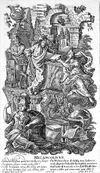
\includegraphics[keepaspectratio,width=0.85\textwidth]{scholar-small.jpg}
  \captionart{Scholar}
  \label{fig:scholar}
\end{figure}

% Force float here
\clearpage{}
\thispagestyle{titleontop}

%SECT. II. MEMB. III. SUBSECT. XV.-_Love of Learning, or overmuch study. With a Digression of the misery of Scholars, and why the Muses are Melancholy_.
\section[Love of Learning, or overmuch study.]{Love of Learning, or overmuch study. With a Digression of the misery of Scholars, and why the Muses are Melancholy.}
\lettrine{L}{eonartus} Fuchsius Instit. lib. \rn{iii.} sect. 1. cap. 1. Felix Plater,
lib. \rn{iii.} de mentis alienat. Herc. de Saxonia, Tract. post. de melanch.
cap. 3, speak of a \authorfootnote{1970}peculiar fury, which comes by overmuch study.
Fernelius, lib. 1, cap. 18, \authorfootnote{1971}puts study, contemplation, and
continual meditation, as an especial cause of madness: and in his 86
consul. cites the same words. Jo. Arculanus, in lib. 9, Rhasis ad
Alnansorem, cap. 16, amongst other causes reckons up studium vehemens:
so doth Levinus Lemnius, lib. de occul. nat. mirac. lib. 1, cap. 16.
\authorfootnote{1972}Many men (saith he) come to this malady by continual study\authormarginnote{1973},
and night-waking, and of all other men, scholars are most subject to
it: and such Rhasis adds, \authorfootnote{1974}that have commonly the finest wits.
Cont. lib. 1, tract. 9, Marsilius Ficinus, de sanit. tuenda, lib. 1.
cap. 7, puts melancholy amongst one of those five principal plagues of
students, 'tis a common Maul unto them all, and almost in some measure
an inseparable companion. Varro belike for that cause calls Tristes
Philosophos et severos, severe, sad, dry, tetric, are common epithets
to scholars: and \authorfootnote{1975}Patritius therefore, in the institution of
princes, would not have them to be great students. For (as Machiavel
holds) study weakens their bodies, dulls the spirits, abates their
strength and courage; and good scholars are never good soldiers, which
a certain Goth well perceived, for when his countrymen came into
Greece, and would have burned all their books, he cried out against it,
by no means they should do it, \authorfootnote{1976} leave them that plague, which in
time will consume all their vigour, and martial spirits. The
\authorfootnote{1977}Turks abdicated Cornutus the next heir from the empire, because
he was so much given to his book: and 'tis the common tenet of the
world, that learning dulls and diminisheth the spirits, and so per
consequens produceth melancholy.

Two main reasons may be given of it, why students should be more
subject to this malady than others. The one is, they live a sedentary,
solitary life, sibi et musis, free from bodily exercise, and those
ordinary disports which other men use: and many times if discontent and
idleness concur with it, which is too frequent, they are precipitated
into this gulf on a sudden: but the common cause is overmuch study; too
much learning (as Festus told\authorfootnote{1978} Paul) hath made thee mad; 'tis that
other extreme which effects it. So did Trincavelius, lib. 1, consil. 12
and 13, find by his experience, in two of his patients, a young baron,
and another that contracted this malady by too vehement study. So
Forestus, observat. l. 10, observ. 13, in a young divine in Louvain,
that was mad, and said \authorfootnote{1979}he had a Bible in his head: Marsilius
Ficinus de sanit. tuend. lib. 1, cap. 1, 3, 4, and lib. 2, cap. 16,
gives many reasons, \authorfootnote{1980} why students dote more often than others.
The first is their negligence; \authorfootnote{1981}other men look to their tools, a
painter will wash his pencils, a smith will look to his hammer, anvil,
forge; a husbandman will mend his plough-irons, and grind his hatchet
if it be dull; a falconer or huntsman will have an especial care of his
hawks, hounds, horses, dogs, \etc{}; a musician will string and unstring
his lute, \etc{}; only scholars neglect that instrument, their brain and
spirits (I mean) which they daily use, and by which they range overall
the world, which by much study is consumed. Vide (saith Lucian) ne
funiculum nimis intendendo aliquando abrumpas: See thou twist not the
rope so hard, till at length it \authorfootnote{1982}break. Facinus in his fourth
chap. gives some other reasons; Saturn and Mercury, the patrons of
learning, they are both dry planets: and Origanus assigns the same
cause, why Mercurialists are so poor, and most part beggars; for that
their president Mercury had no better fortune himself. The destinies of
old put poverty upon him as a punishment; since when, poetry and
beggary are Gemelli, twin-born brats, inseparable companions;
\authorfootnote{1983}And to this day is every scholar poor;
Gross gold from them runs headlong to the boor:

Mercury can help them to knowledge, but not to money. The second is
contemplation, \authorfootnote{1984}which dries the brain and extinguisheth natural
heat; for whilst the spirits are intent to meditation above in the
head, the stomach and liver are left destitute, and thence come black
blood and crudities by defect of concoction, and for want of exercise
the superfluous vapours cannot exhale, \etc{}. The same reasons are
repeated by Gomesius, lib. 4, cap. 1, de sale \authorfootnote{1985}Nymannus orat. de
Imag. Jo. Voschius, lib. 2, cap. 5, de peste: and something more they
add, that hard students are commonly troubled with gouts, catarrhs,
rheums, cachexia, bradiopepsia, bad eyes, stone and colic,
\authorfootnote{1986}crudities, oppilations, vertigo, winds, consumptions, and all
such diseases as come by overmuch sitting; they are most part lean,
dry, ill-coloured, spend their fortunes, lose their wits, and many
times their lives, and all through immoderate pains, and extraordinary
studies. If you will not believe the truth of this, look upon great
Tostatus and Thomas Aquinas's works, and tell me whether those men took
pains? peruse \Austin{}, Hierom, \etc{}, and many thousands besides.
Qui cupit optatam cursu contingere metam,
Multa tulit, fecitque puer, sudavit et alsit.

He that desires this wished goal to gain,
Must sweat and freeze before he can attain,

and labour hard for it. So did \Seneca, by his own confession, ep. 8.
\authorfootnote{1987}Not a day that I spend idle, part of the night I keep mine eyes
open, tired with waking, and now slumbering to their continual task.
Hear Tully pro Archia Poeta: whilst others loitered, and took their
pleasures, he was continually at his book, so they do that will be
scholars, and that to the hazard (I say) of their healths, fortunes,
wits, and lives. How much did \Aristotle and Ptolemy spend? unius regni
precium they say, more than a king's ransom; how many crowns per annum,
to perfect arts, the one about his History of Creatures, the other on
his Almagest? How much time did Thebet Benchorat employ, to find out
the motion of the eighth sphere? forty years and more, some write: how
many poor scholars have lost their wits, or become dizzards, neglecting
all worldly affairs and their own health, wealth, esse and bene esse,
to gain knowledge for which, after all their pains, in this world's
esteem they are accounted ridiculous and silly fools, idiots, asses,
and (as oft they are) rejected, contemned, derided, doting, and mad.
Look for examples in Hildesheim spicel. 2, de mania et delirio: read
Trincavellius, l. 3. consil. 36, et c. 17. Montanus, consil. 233.
\authorfootnote{1988}Garceus de Judic. genit. cap. 33. Mercurialis, consil. 86, cap.
25. Prosper \authorfootnote{1989}Calenius in his Book de atra bile; Go to Bedlam and
ask. Or if they keep their wits, yet they are esteemed scrubs and fools
by reason of their carriage: after seven years' study
---statua, taciturnius exit,
Plerumque et risum populi quatit.---

He becomes more silent than a statue, and generally excites people's
laughter. Because they cannot ride a horse, which every clown can do;
salute and court a gentlewoman, carve at table, cringe and make conges,
which every common swasher can do, \authorfootnote{1990}hos populus ridet, \etc{}, they
are laughed to scorn, and accounted silly fools by our gallants. Yea,
many times, such is their misery, they deserve it: \authorfootnote{1991}a mere
scholar, a mere ass.
\authorfootnote{1992}Obstipo capite, et figentes lumine terram,
Murmura cum secum, et rabiosa silentia rodunt,
Atque experrecto trutinantur verba labello,
Aegroti veteris meditantes somnia, gigni
De nihilo nihilum; in nihilum nil posse reverti.

\authorfootnote{1993}---who do lean awry
Their heads, piercing the earth with a fixt eye;
When, by themselves, they gnaw their murmuring,
And furious silence, as 'twere balancing
Each word upon their out-stretched lip, and when
They meditate the dreams of old sick men,
As, 'Out of nothing, nothing can be brought;
And that which is, can ne'er be turn'd to nought.'

Thus they go commonly meditating unto themselves, thus they sit, such
is their action and gesture. Fulgosus, l. 8, c. 7, makes mention how
Th. Aquinas supping with king Lewis of France, upon a sudden knocked
his fist upon the table, and cried, conclusum est contra Manichaeos,
his wits were a wool-gathering, as they say, and his head busied about
other matters, when he perceived his error, he was much \authorfootnote{1994}abashed.
Such a story there is of Archimedes in Vitruvius, that having found out
the means to know how much gold was mingled with the silver in king
Hieron's crown, ran naked forth of the bath and cried ἕυρηκα, I have
found: \authorfootnote{1995}and was commonly so intent to his studies, that he never
perceived what was done about him: when the city was taken, and the
soldiers now ready to rifle his house, he took no notice of it. St.
Bernard rode all day long by the Lemnian lake, and asked at last where
he was, Marullus, lib. 2, cap. 4. It was \Democritus{}'s carriage alone
that made the Abderites suppose him to have been mad, and send for
Hippocrates to cure him: if he had been in any solemn company, he would
upon all occasions fall a laughing. Theophrastus saith as much of
Heraclitus, for that he continually wept, and Laertius of Menedemus
Lampsacus, because he ran like a madman, \authorfootnote{1996}saying, he came from
hell as a spy, to tell the devils what mortal men did. Your greatest
students are commonly no better, silly, soft fellows in their outward
behaviour, absurd, ridiculous to others, and no whit experienced in
worldly business; they can measure the heavens, range over the world,
teach others wisdom, and yet in bargains and contracts they are
circumvented by every base tradesman. Are not these men fools? and how
should they be otherwise, but as so many sots in schools, when (as
\authorfootnote{1997}he well observed) they neither hear nor see such things as are
commonly practised abroad? how should they get experience, by what
means? \authorfootnote{1998}I knew in my time many scholars, saith Aeneas Sylvius (in
an epistle of his to Gasper Scitick, chancellor to the emperor),
excellent well learned, but so rude, so silly, that they had no common
civility, nor knew how to manage their domestic or public affairs.
Paglarensis was amazed, and said his farmer had surely cozened him,
when he heard him tell that his sow had eleven pigs, and his ass had
but one foal. To say the best of this profession, I can give no other
testimony of them in general, than that of \Pliny{} of Isaeus; \authorfootnote{1999}He is
yet a scholar, than which kind of men there is nothing so simple, so
sincere, none better, they are most part harmless, honest, upright,
innocent, plain-dealing men.

Now because they are commonly subject to such hazards and
inconveniences as dotage, madness, simplicity, \etc{}. Jo. Voschius would
have good scholars to be highly rewarded, and had in some extraordinary
respect above other men, to have greater \authorfootnote{2000}privileges than the
rest, that adventure themselves and abbreviate their lives for the
public good. But our patrons of learning are so far nowadays from
respecting the muses, and giving that honour to scholars, or reward
which they deserve, and are allowed by those indulgent privileges of
many noble princes, that after all their pains taken in the
universities, cost and charge, expenses, irksome hours, laborious
tasks, wearisome days, dangers, hazards, (barred interim from all
pleasures which other men have, mewed up like hawks all their lives) if
they chance to wade through them, they shall in the end be rejected,
contemned, and which is their greatest misery, driven to their shifts,
exposed to want, poverty, and beggary. Their familiar attendants are,
\authorfootnote{2001}Pallentes morbi, luctus, curaeque laborque
Et metus, et malesuada fames, et turpis egestas,
Terribiles visu formae---

Grief, labour, care, pale sickness, miseries,
Fear, filthy poverty, hunger that cries,
Terrible monsters to be seen with eyes.

If there were nothing else to trouble them, the conceit of this alone
were enough to make them all melancholy. Most other trades and
professions, after some seven years' apprenticeship, are enabled by
their craft to live of themselves. A merchant adventures his goods at
sea, and though his hazard be great, yet if one ship return of four, he
likely makes a saving voyage. An husbandman's gains are almost certain;
quibus ipse Jupiter nocere non potest (whom Jove himself can't harm)
('tis \authorfootnote{2002}Cato's hyperbole, a great husband himself); only scholars
methinks are most uncertain, unrespected, subject to all casualties,
and hazards. For first, not one of a many proves to be a scholar, all
are not capable and docile, \authorfootnote{2003}ex omniligno non fit Mercurius: we
can make majors and officers every year, but not scholars: kings can
invest knights and barons, as Sigismund the emperor confessed;
universities can give degrees; and Tu quod es, e populo quilibet esse
potest; but he nor they, nor all the world, can give learning, make
philosophers, artists, orators, poets; we can soon say, as \Seneca well
notes, O virum bonum, o divitem, point at a rich man, a good, a happy
man, a prosperous man, sumptuose vestitum, Calamistratum, bene olentem,
magno temporis impendio constat haec laudatio, o virum literarum, but
'tis not so easily performed to find out a learned man. Learning is not
so quickly got, though they may be willing to take pains, to that end
sufficiently informed, and liberally maintained by their patrons and
parents, yet few can compass it. Or if they be docile, yet all men's
wills are not answerable to their wits, they can apprehend, but will
not take pains; they are either seduced by bad companions, vel in
puellam impingunt, vel in poculum (they fall in with women or wine) and
so spend their time to their friends' grief and their own undoings. Or
put case they be studious, industrious, of ripe wits, and perhaps good
capacities, then how many diseases of body and mind must they
encounter? No labour in the world like unto study. It may be, their
temperature will not endure it, but striving to be excellent to know
all, they lose health, wealth, wit, life and all. Let him yet happily
escape all these hazards, aereis intestinis with a body of brass, and
is now consummate and ripe, he hath profited in his studies, and
proceeded with all applause: after many expenses, he is fit for
preferment, where shall he have it? he is as far to seek it as he was
(after twenty years' standing) at the first day of his coming to the
University. For what course shall he take, being now capable and ready?
The most parable and easy, and about which many are employed, is to
teach a school, turn lecturer or curate, and for that he shall have
falconer's wages, ten pound per annum, and his diet, or some small
stipend, so long as he can please his patron or the parish; if they
approve him not (for usually they do but a year or two) as inconstant,
as they that cried\authorfootnote{2004} Hosanna one day, and Crucify him the other;
serving-man-like, he must go look a new master; if they do, what is his
reward?
\authorfootnote{2005}\li{Hoc quoque te manet ut pueros elementa docentem
Occupet extremis in vicis alba senectus.}

At last thy snow-white age in suburb schools,
Shall toil in teaching boys their grammar rules.

Like an ass, he wears out his time for provender, and can show a stump
rod, togam tritam et laceram saith \authorfootnote{2006}Haedus, an old torn gown, an
ensign of his infelicity, he hath his labour for his pain, a modicum to
keep him till he be decrepit, and that is all. Grammaticus non est
felix, \etc{}. If he be a trencher chaplain in a gentleman's house, as it
befell \authorfootnote{2007} Euphormio, after some seven years' service, he may
perchance have a living to the halves, or some small rectory with the
mother of the maids at length, a poor kinswoman, or a cracked
chambermaid, to have and to hold during the time of his life. But if he
offend his good patron, or displease his lady mistress in the mean
time,
\authorfootnote{2008}Ducetur Planta velut ictus ab Hercule Cacus,
Poneturque foras, si quid tentaverit unquam
Hiscere---

as Hercules did by Cacus, he shall be dragged forth of doors by the
heels, away with him. If he bend his forces to some other studies, with
an intent to be a secretis to some nobleman, or in such a place with an
ambassador, he shall find that these persons rise like apprentices one
under another, and in so many tradesmen's shops, when the master is
dead, the foreman of the shop commonly steps in his place. Now for
poets, rhetoricians, historians, philosophers, \authorfootnote{2009}mathematicians,
sophisters, \etc{}; they are like grasshoppers, sing they must in summer,
and pine in the winter, for there is no preferment for them. Even so
they were at first, if you will believe that pleasant tale of Socrates,
which he told fair Phaedrus under a plane-tree, at the banks of the
river Iseus; about noon when it was hot, and the grasshoppers made a
noise, he took that sweet occasion to tell him a tale, how grasshoppers
were once scholars, musicians, poets, \etc{}, before the Muses were born,
and lived without meat and drink, and for that cause were turned by
Jupiter into grasshoppers. And may be turned again, In Tythoni Cicadas,
aut Lyciorum ranas, for any reward I see they are like to have: or else
in the mean time, I would they could live, as they did, without any
viaticum, like so many \authorfootnote{2010}manucodiatae, those Indian birds of
paradise, as we commonly call them, those I mean that live with the air
and dew of heaven, and need no other food; for being as they are, their
\authorfootnote{2011}rhetoric only serves them to curse their bad fortunes, and many
of them for want of means are driven to hard shifts; from grasshoppers
they turn humble-bees and wasps, plain parasites, and make the muses,
mules, to satisfy their hunger-starved paunches, and get a meal's meat.
To say truth, 'tis the common fortune of most scholars, to be servile
and poor, to complain pitifully, and lay open their wants to their
respectless patrons, as Cardan doth\authorfootnote{2012}, as Xilander\authorfootnote{2013} and many
others: and which is too common in those dedicatory epistles, for hope
of gain, to lie, flatter, and with hyperbolical eulogiums and
commendations, to magnify and extol an illiterate unworthy idiot, for
his excellent virtues, whom they should rather, as Machiavel
observes\authorfootnote{2014}, vilify, and rail at downright for his most notorious
villainies and vices. So they prostitute themselves as fiddlers, or
mercenary tradesmen, to serve great men's turns for a small reward.
They are like Indians, they have store of gold, but know not the
worth of it\authormarginnote{2015}: for I am of Synesius's opinion, \authorfootnote{2016}King Hieron got more
by Simonides' acquaintance, than Simonides did by his; they have their
best education, good institution, sole qualification from us, and when
they have done well, their honour and immortality from us: we are the
living tombs, registers, and as so many trumpeters of their fames: what
was Achilles without Homer? Alexander without Arian and Curtius? who
had known the Caesars, but for Suetonius and Dion?
\authorfootnote{2017}Vixerunt fortes ante Agamemnona
Multi: sed omnes illachrymabiles
Urgentur, ignotique longa
Nocte, carent quia vate sacro.

Before great Agamemnon reign'd,
Reign'd kings as great as he, and brave,

Whose huge ambition's now contain'd
In the small compass of a grave:

In endless night, they sleep, unwept, unknown,
No bard they had to make all time their own.

they are more beholden to scholars, than scholars to them; but they
undervalue themselves, and so by those great men are kept down. Let
them have that encyclopaedian, all the learning in the world; they must
keep it to themselves, \authorfootnote{2018}live in base esteem, and starve, except
they will submit, as Budaeus well hath it, so many good parts, so many
ensigns of arts, virtues, be slavishly obnoxious to some illiterate
potentate, and live under his insolent worship, or honour, like
parasites, Qui tanquam mures alienum panem comedunt. For to say truth,
artes hae, non sunt Lucrativae, as Guido Bonat that great astrologer
could foresee, they be not gainful arts these, sed esurientes et
famelicae, but poor and hungry.

\authorfootnote{2019}Dat Galenus opes, dat Justinianus honores,
Sed genus et species cogitur ire pedes:


The rich physician, honour'd lawyers ride,
Whilst the poor scholar foots it by their side.

Poverty is the muses' patrimony, and as that poetical divinity teacheth
us, when Jupiter's daughters were each of them married to the gods, the
muses alone were left solitary, Helicon forsaken of all suitors, and I
believe it was, because they had no portion.

Calliope longum caelebs cur vixit in aevum?
Nempe nihil dotis, quod numeraret, erat.


Why did Calliope live so long a maid?
Because she had no dowry to be paid.

Ever since all their followers are poor, forsaken and left unto
themselves. Insomuch, that as Petronius argues\authorfootnote{2020}, you shall likely
know them by their clothes. There came, saith he, by chance into my
company, a fellow not very spruce to look on, that I could perceive by
that note alone he was a scholar, whom commonly rich men hate: I asked
him what he was, he answered, a poet: I demanded again why he was so
ragged, he told me this kind of learning never made any man rich.
\authorfootnote{2021}Qui Pelago credit, magno se faenore tollit,
Qui pugnas et rostra petit, praecingitur auro:
Vilis adulator picto jacet ebrius ostro,
Sola pruinosis horret facundia pannis.


A merchant's gain is great, that goes to sea;
A soldier embossed all in gold;

A flatterer lies fox'd in brave array;
A scholar only ragged to behold.

All which our ordinary students, right well perceiving in the
universities, how unprofitable these poetical, mathematical, and
philosophical studies are, how little respected, how few patrons; apply
themselves in all haste to those three commodious professions of law,
physic, and divinity, sharing themselves between them, \authorfootnote{2022}rejecting
these arts in the mean time, history, philosophy, philology, or lightly
passing them over, as pleasant toys fitting only table-talk, and to
furnish them with discourse. They are not so behoveful: he that can
tell his money hath arithmetic enough: he is a true geometrician, can
measure out a good fortune to himself; a perfect astrologer, that can
cast the rise and fall of others, and mark their errant motions to his
own use. The best optics are, to reflect the beams of some great man's
favour and grace to shine upon him. He is a good engineer that alone
can make an instrument to get preferment. This was the common tenet and
practice of Poland, as Cromerus observed not long since, in the first
book of his history; their universities were generally base, not a
philosopher, a mathematician, an antiquary, \etc{}, to be found of any
note amongst them, because they had no set reward or stipend, but every
man betook himself to divinity, hoc solum in votis habens, opimum
sacerdotium, a good parsonage was their aim. This was the practice of
some of our near neighbours, as Lipsius inveighs\authorfootnote{2023}, they thrust
their children to the study of law and divinity, before they be
informed aright, or capable of such studies. Scilicet omnibus artibus
antistat spes lucri, et formosior est cumulus auri, quam quicquid
Graeci Latinique delirantes scripserunt. Ex hoc numero deinde veniunt
ad gubernacula reipub. intersunt et praesunt consiliis regum, o pater,
o patria? so he complained, and so may others. For even so we find, to
serve a great man, to get an office in some bishop's court (to practise
in some good town) or compass a benefice, is the mark we shoot at, as
being so advantageous, the highway to preferment.

Although many times, for aught I can see, these men fail as often as
the rest in their projects, and are as usually frustrate of their
hopes. For let him be a doctor of the law, an excellent civilian of
good worth, where shall he practise and expatiate? Their fields are so
scant, the civil law with us so contracted with prohibitions, so few
causes, by reason of those all-devouring municipal laws, \li{quibus nihil
illiteratius}, saith Erasmus\authorfootnote{2024}, an illiterate and a barbarous
study, (for though they be never so well learned in it, I can hardly
vouchsafe them the name of scholars, except they be otherwise
qualified) and so few courts are left to that profession, such slender
offices, and those commonly to be compassed at such dear rates, that I
know not how an ingenious man should thrive amongst them. Now for
physicians, there are in every village so many mountebanks, empirics,
quacksalvers, Paracelsians, as they call themselves, Caucifici et
sanicidae so Clenard terms them\authorfootnote{2025}, wizards, alchemists, poor
vicars, cast apothecaries, physicians' men, barbers, and good wives,
professing great skill, that I make great doubt how they shall be
maintained, or who shall be their patients. Besides, there are so many
of both sorts, and some of them such harpies, so covetous, so
clamorous, so impudent; and as he said\authorfootnote{2026}, litigious idiots,

\begin{latin}%
Quibus loquacis affatim arrogantiae est
Pentiae parum aut nihil,

Nec ulla mica literarii salis,
Crumenimulga natio:

Loquuteleia turba, litium strophae,
Maligna litigantium cohors, togati vultures,

Lavernae alumni, Agyrtae, \etc{}.%
\end{latin}

Which have no skill but prating arrogance,
No learning, such a purse-milking nation:

Gown'd vultures, thieves, and a litigious rout
Of cozeners, that haunt this occupation,

that they cannot well tell how to live one by another, but as he jested
in the Comedy of Clocks, they were so many, \authorfootnote{2027}major pars populi
arida reptant fame, they are almost starved a great part of them, and
ready to devour their fellows, \authorfootnote{2028}\li{Et noxia callidilate se corripere},
such a multitude of pettifoggers and empirics, such impostors, that an
honest man knows not in what sort to compose and behave himself in
their society, to carry himself with credit in so vile a rout,
\li{scientiae nomen, tot sumptibus partum et vigiliis, profiteri dispudeat,
postquam, \etc{}}.

Last of all to come to our divines, the most noble profession and
worthy of double honour, but of all others the most distressed and
miserable. If you will not believe me, hear a brief of it, as it was
not many years since publicly preached at Paul's cross, \authorfootnote{2029}by a
grave minister then, and now a reverend bishop of this land: We that
are bred up in learning, and destinated by our parents to this end, we
suffer our childhood in the grammar-school, which \Austin{} calls magnam
tyrannidem, et grave malum, and compares it to the torments of
martyrdom; when we come to the university, if we live of the college
allowance, as Phalaris objected to the Leontines, \textgreek{παν τῶν ἐνδεῖς πλὴν
λιμοὺ καὶ φόβου}, needy of all things but hunger and fear, or if we be
maintained but partly by our parents' cost, do expend in unnecessary
maintenance, books and degrees, before we come to any perfection, five
hundred pounds, or a thousand marks. If by this price of the expense of
time, our bodies and spirits, our substance and patrimonies, we cannot
purchase those small rewards, which are ours by law, and the right of
inheritance, a poor parsonage, or a vicarage of 50\emph{l.} per annum, but
we must pay to the patron for the lease of a life (a spent and out-worn
life) either in annual pension, or above the rate of a copyhold, and
that with the hazard and loss of our souls, by simony and perjury, and
the forfeiture of all our spiritual preferments, in esse and posse,
both present and to come. What father after a while will be so
improvident to bring up his son to his great charge, to this necessary
beggary? What Christian will be so irreligious, to bring up his son in
that course of life, which by all probability and necessity, cogit ad
turpia, enforcing to sin, will entangle him in simony and perjury, when
as the poet said, \li{Invitatus ad haec aliquis de ponte negabit}: a
beggar's brat taken from the bridge where he sits a begging, if he knew
the inconvenience, had cause to refuse it. This being thus, have not we
fished fair all this while, that are initiate divines, to find no
better fruits of our labours, \authorfootnote{2030} hoc est cur palles, cur quis non
prandeat hoc est? do we macerate ourselves for this? Is it for this we
rise so early all the year long? \authorfootnote{2031}Leaping (as he saith) out of our
beds, when we hear the bell ring, as if we had heard a thunderclap. If
this be all the respect, reward and honour we shall have, \authorfootnote{2032}frange
leves calamos, et scinde Thalia libellos: let us give over our books,
and betake ourselves to some other course of life; to what end should
we study? \authorfootnote{2033}\li{Quid me litterulas stulti docuere parentes}, what did
our parents mean to make us scholars, to be as far to seek of
preferment after twenty years' study, as we were at first: why do we
take such pains? Quid tantum insanis juvat impallescere chartis? If
there be no more hope of reward, no better encouragement, I say again,
\li{Frange leves calamos, et scinde Thalia libellos}; let's turn soldiers,
sell our books, and buy swords, guns, and pikes, or stop bottles with
them, turn our philosopher's gowns, as Cleanthes once did, into
millers' coats, leave all and rather betake ourselves to any other
course of life, than to continue longer in this misery. \authorfootnote{2034}\li{Praestat
dentiscalpia radere, quam literariis monumentis magnatum favorem
emendicare}.

Yea, but methinks I hear some man except at these words, that though
this be true which I have said of the estate of scholars, and
especially of divines, that it is miserable and distressed at this
time, that the church suffers shipwreck of her goods, and that they
have just cause to complain; there is a fault, but whence proceeds it?
If the cause were justly examined, it would be retorted upon ourselves,
if we were cited at that tribunal of truth, we should be found guilty,
and not able to excuse it That there is a fault among us, I confess,
and were there not a buyer, there would not be a seller; but to him
that will consider better of it, it will more than manifestly appear,
that the fountain of these miseries proceeds from these griping
patrons. In accusing them, I do not altogether excuse us; both are
faulty, they and we: yet in my judgment, theirs is the greater fault,
more apparent causes and much to be condemned. For my part, if it be
not with me as I would, or as it should, I do ascribe the cause, as
\authorfootnote{2035}Cardan did in the like case; \li{meo infortunio potius quam illorum
sceleri}, to \authorfootnote{2036}mine own infelicity rather than their naughtiness:
although I have been baffled in my time by some of them, and have as
just cause to complain as another: or rather indeed to mine own
negligence; for I was ever like that Alexander in \authorfootnote{2037}Plutarch,
Crassus his tutor in philosophy, who, though he lived many years
familiarly with rich Crassus, was even as poor when from, (which many
wondered at) as when he came first to him; he never asked, the other
never gave him anything; when he travelled with Crassus he borrowed a
hat of him, at his return restored it again. I have had some such noble
friends' acquaintance and scholars, but most part (common courtesies
and ordinary respects excepted) they and I parted as we met, they gave
me as much as I requested, and that was-And as Alexander ab Alexandro
Genial. dier. l. 6. c. 16. made answer to Hieronymus Massainus, that
wondered, \li{quum plures ignavos et ignobiles ad dignitates et sacerdotia
promotos quotidie videret}, when other men rose, still he was in the
same state, \li{eodem tenore et fortuna cui mercedem laborum studiorumque
deberi putaret}, whom he thought to deserve as well as the rest. He made
answer, that he was content with his present estate, was not ambitious,
and although \li{objurgabundus suam segnitiem accusaret, cum obscurae
sortis homines ad sacerdotia et pontificatus evectos, \etc{},} he chid him
for his backwardness, yet he was still the same: and for my part
(though I be not worthy perhaps to carry Alexander's books) yet by some
overweening and well-wishing friends, the like speeches have been used
to me; but I replied still with Alexander, that I had enough, and more
peradventure than I deserved; and with Libanius Sophista, that rather
chose (when honours and offices by the emperor were offered unto him)
to be talis Sophista, \li{quam tails Magistratus}. I had as lief be still
\Democritus{} junior, and \li{privus privatus, si mihi jam daretur optio, quam
talis fortasse Doctor, talis Dominus.-Sed quorsum haec?} For the rest
'tis on both sides facinus detestandum, to buy and sell livings, to
detain from the church, that which God's and men's laws have bestowed
on it; but in them most, and that from the covetousness and ignorance
of such as are interested in this business; I name covetousness in the
first place, as the root of all these mischiefs, which, Achan-like,
compels them to commit sacrilege, and to make simoniacal compacts, (and
what not) to their own ends, \authorfootnote{2038}that kindles God's wrath, brings a
plague, vengeance, and a heavy visitation upon themselves and others.
Some out of that insatiable desire of filthy lucre, to be enriched,
care not how they come by it per fas et nefas, hook or crook, so they
have it. And others when they have with riot and prodigality embezzled
their estates, to recover themselves, make a prey of the church,
robbing it, as Julian the apostate did\authorfootnote{2039}, spoil parsons of their
revenues (in keeping half back, \authorfootnote{2040}as a great man amongst us
observes:) and that maintenance on which they should live: by means
whereof, barbarism is increased, and a great decay of Christian
professors: for who will apply himself to these divine studies, his
son, or friend, when after great pains taken, they shall have nothing
whereupon to live? But with what event do they these things?
\authormarginnote{2041}\li{Opesque totis viribus venamini
At inde messis accidit miserrima.}

They toil and moil, but what reap they? They are commonly unfortunate
families that use it, accursed in their pro\-geny, and, as common
experience evinceth, accursed themselves in all their proceedings. With
what face (as he quotes\authorfootnote{2042} out of Aust.) can they expect a blessing
or inheritance from Christ in heaven, that defraud Christ of his
inheritance here on earth? I would all our simoniacal patrons, and such
as detain tithes, would read those judicious tracts of Sir Henry
Spelman, and Sir James Sempill, knights; those late elaborate and
learned treatises of Dr. Tilslye, and Mr. Montague, which they have
written of that subject. But though they should read, it would be to
small purpose, clames licet et mare coelo Confundas; thunder, lighten,
preach hell and damnation, tell them 'tis a sin, they will not believe
it; denounce and terrify, they have \authorfootnote{2043}cauterised consciences, they
do not attend, as the enchanted adder, they stop their ears. Call them
base, irreligious, profane, barbarous, pagans, atheists, epicures, (as
some of them surely are) with the bawd in \Plautus{}, Euge, optime, they
cry and applaud themselves with that miser, \authorfootnote{2044}simul ac nummos
contemplor in arca: say what you will, quocunque modo rem: as a dog
barks at the moon, to no purpose are your sayings: Take your heaven,
let them have money. A base, profane, epicurean, hypocritical rout: for
my part, let them pretend what zeal they will, counterfeit religion,
blear the world's eyes, bombast themselves, and stuff out their
greatness with church spoils, shine like so many peacocks; so cold is
my charity, so defective in this behalf, that I shall never think
better of them, than that they are rotten at core, their bones are full
of epicurean hypocrisy, and atheistical marrow, they are worse than
heathens. For as Dionysius Halicarnassaeus observes, Antiq. Rom. lib.
7. \authorfootnote{2045}\li{Primum locum, \etc{}.} Greeks and Barbarians observe all religious
rites, and dare not break them for fear of offending their gods; but
our simoniacal contractors, our senseless Achans, our stupefied
patrons, fear neither God nor devil, they have evasions for it, it is
no sin, or not due jure divino, or if a sin, no great sin, \etc{}. And
though they be daily punished for it, and they do manifestly perceive,
that as he said, frost and fraud come to foul ends; yet as
\authorfootnote{2046}\Chrysostom{} follows it \li{Nulla ex poena sit correctio, et quasi
adversis malitia hominum provocetur, crescit quotidie quod puniatur}:
they are rather worse than better,-\li{iram atque animos a crimine sumunt},
and the more they are corrected, the more they offend: but let them
take their course, \authorfootnote{2047}\li{Rode caper vites}, go on still as they begin,
'tis no sin, let them rejoice secure, God's vengeance will overtake
them in the end, and these ill-gotten goods, as an eagle's feathers,
\authorfootnote{2048} will consume the rest of their substance; it is \authorfootnote{2049}\li{aurum
Tholosanum}, and will produce no better effects. \authorfootnote{2050}Let them lay it
up safe, and make their conveyances never so close, lock and shut door,
saith \Chrysostom{}, yet fraud and covetousness, two most violent thieves
are still included, and a little gain evil gotten will subvert the rest
of their goods. The eagle in Aesop, seeing a piece of flesh now ready
to be sacrificed, swept it away with her claws, and carried it to her
nest; but there was a burning coal stuck to it by chance, which
unawares consumed her young ones, nest, and all together. Let our
simoniacal church-chopping patrons, and sacrilegious harpies, look for
no better success.

A second cause is ignorance, and from thence contempt, \li{successit odium
in literas ab ignorantia vulgi}; which \authorfootnote{2051}Junius well perceived: this
hatred and contempt of learning proceeds out of \authorfootnote{2052}ignorance; as
they are themselves barbarous, idiots, dull, illiterate, and proud, so
they esteem of others. \li{Sint Mecaenates, non deerunt Flacce Marones}: Let
there be bountiful patrons, and there will be painful scholars in all
sciences. But when they contemn learning, and think themselves
sufficiently qualified, if they can write and read, scramble at a piece
of evidence, or have so much Latin as that emperor had, \li{qui
nescit dissimulare, nescit vivere}\authorlatintrans{2053}, they are unfit to do their country
service, to perform or undertake any action or employment, which may
tend to the good of a commonwealth, except it be to fight, or to do
country justice, with common sense, which every yeoman can likewise do.
And so they bring up their children, rude as they are themselves,
unqualified, untaught, uncivil most part. \authormarginnote{2054}\li{Quis e nostra juventute
legitime instituitur literis? Quis oratores aut Philosophos tangit?
quis historiam legit, illam rerum agendarum quasi animam? praecipitant
parentes vota sua, \etc{}.} 'twas Lipsius' complaint to his illiterate
countrymen, it may be ours. Now shall these men judge of a scholar's
worth, that have no worth, that know not what belongs to a student's
labours, that cannot distinguish between a true scholar and a drone? or
him that by reason of a voluble tongue, a strong voice, a pleasing
tone, and some trivially polyanthean helps, steals and gleans a few
notes from other men's harvests, and so makes a fairer show, than he
that is truly learned indeed: that thinks it no more to preach, than to
speak, \authorfootnote{2055}or to run away with an empty cart; as a grave man said:
and thereupon vilify us, and our pains; scorn us, and all learning.
\authorfootnote{2056} Because they are rich, and have other means to live, they think
it concerns them not to know, or to trouble themselves with it; a
fitter task for younger brothers, or poor men's sons, to be pen and
inkhorn men, pedantical slaves, and no whit beseeming the calling of a
gentleman, as Frenchmen and Germans commonly do, neglect therefore all
human learning, what have they to do with it? Let mariners learn
astronomy; merchants, factors study arithmetic; surveyors get them
geometry; spectacle-makers optics; land-leapers geography; town-clerks
rhetoric, what should he do with a spade, that hath no ground to dig;
or they with learning, that have no use of it? thus they reason, and
are not ashamed to let mariners, apprentices, and the basest servants,
be better qualified than themselves. In former times, kings, princes,
and emperors, were the only scholars, excellent in all faculties.
Julius Caesar mended the year, and writ his own Commentaries,
\authorfootnote{2057}---\li{media inter prealia semper,
Stellarum coelique plagis, superisque vacavit}.

\authorfootnote{2058}Antonius, Adrian, Nero, Seve. Jul. \etc{}. \authorfootnote{2059}Michael the emperor,
and Isacius, were so much given to their studies, that no base fellow
would take so much pains: Orion, Perseus, Alphonsus, Ptolomeus, famous
astronomers; Sabor, Mithridates, Lysimachus, admired physicians:
Plato's kings all: Evax, that Arabian prince, a most expert jeweller,
and an exquisite philosopher; the kings of Egypt were priests of old,
chosen and from thence,-Idem rex hominum, Phoebique sacerdos: but those
heroical times are past; the Muses are now banished in this bastard
age, \li{ad sordida tuguriola}, to meaner persons, and confined alone almost
to universities. In those days, scholars were highly beloved,
\authorfootnote{2060}honoured, esteemed; as old Ennius by Scipio Africanus, \Virgil{} by
Augustus; \Horace{} by Meceanas: princes' companions; dear to them, as
Anacreon to Polycrates; Philoxenus to Dionysius, and highly rewarded.
Alexander sent Xenocrates the philosopher fifty talents, because he was
poor, \li{visu rerum, aut eruditione praestantes viri, mensis olim regum
adhibiti}, as Philostratus relates of Adrian and Lampridius of Alexander
Severus: famous clerks came to these princes' courts, velut in Lycaeum,
as to a university, and were admitted to their tables, \li{quasi divum
epulis accumbentes}; Archilaus, that Macedonian king, would not
willingly sup without Euripides, (amongst the rest he drank to him at
supper one night, and gave him a cup of gold for his pains) delectatus
poetae suavi sermone; and it was fit it should be so; because as
\authorfootnote{2061}Plato in his Protagoras well saith, a good philosopher as much
excels other men, as a great king doth the commons of his country; and
again, \authorfootnote{2062}\li{quoniam illis nihil deest, et minime egere solent, et
disciplinas quas profitentur, soli a contemptu vindicare possunt}, they
needed not to beg so basely, as they compel \authorfootnote{2063}scholars in our times
to complain of poverty, or crouch to a rich chuff for a meal's meat,
but could vindicate themselves, and those arts which they professed.
Now they would and cannot: for it is held by some of them, as an axiom,
that to keep them poor, will make them study; they must be dieted, as
horses to a race, not pampered, \authorfootnote{2064}\li{Alendos volunt, non saginandos,
ne melioris mentis flammula extinguatur}; a fat bird will not sing, a
fat dog cannot hunt, and so by this depression of theirs \authorfootnote{2065}some
want means, others will, all want \authorfootnote{2066}encouragement, as being
forsaken almost; and generally contemned. 'Tis an old saying, \li{Sint
Mecaenates, non deerunt Flacce Marones}, and 'tis a true saying still.
Yet oftentimes I may not deny it the main fault is in ourselves. Our
academics too frequently offend in neglecting patrons, as Erasmus
well taxet\authorfootnote{2067}h, or making ill choice of them; \li{negligimus oblatos aut
amplectimur parum aptos}, or if we get a good one, \li{non studemus mutuis
officiis favorem ejus alere}, we do not ply and follow him as we should.
\li{Idem mihi accidit Adolescenti} (saith Erasmus) acknowledging his fault,
\li{et gravissime peccavi}, and so may I say myself\authormarginnote{2068}, I have offended
in this, and so peradventure have many others. We did not spondere
\li{magnatum favoribus, qui caeperunt nos amplecti}, apply ourselves with
that readiness we should: idleness, love of liberty, \li{immodicus amor
libertatis effecit ut diu cum perfidis amicis}, as he confesseth, et
pertinaci pauperate colluctarer, bashfulness, melancholy, timorousness,
cause many of us to be too backward and remiss. So some offend in one
extreme, but too many on the other, we are most part too forward, too
solicitous, too ambitious, too impudent; we commonly complain deesse
Maecenates, of want of encouragement, want of means, when as the true
defect is in our own want of worth, our insufficiency: did Maecenas
take notice of \Horace{} or \Virgil{} till they had shown themselves first?
or had Bavius and Mevius any patrons? \li{Egregium specimen dent}, saith
Erasmus, let them approve themselves worthy first, sufficiently
qualified for learning and manners, before they presume or impudently
intrude and put themselves on great men as too many do, with such base
flattery, parasitical colloguing, such hyperbolical elogies they do
usually insinuate that it is a shame to hear and see. Immodicae laudes
conciliant invidiam, potius quam laudem, and vain commendations
derogate from truth, and we think in conclusion, non melius de laudato,
pejus de laudante, ill of both, the commender and commended. So we
offend, but the main fault is in their harshness, defect of patrons.
How beloved of old, and how much respected was Plato to Dionysius? How
dear to Alexander was \Aristotle, Demeratus to Philip, Solon to Croesus,
Auexarcus and Trebatius to Augustus, Cassius to Vespasian, Plutarch to
Trajan, \Seneca to Nero, Simonides to Hieron? how honoured?
\li{Sed haec prius fuere, nunc recondita
Senent quiete}\authorfootnote{2069},

those days are gone; \li{Et spes, et ratio studiorum in Caesare
tantum}\authorlatintrans{2070}: as he said of old, we may truly say now, he is
our amulet, our \authorfootnote{2071}sun, our sole comfort and refuge, our Ptolemy, our common
Maecenas, \li{Jacobus munificus, Jacobus pacificus, mysta Musarum, Rex
Platonicus: Grande decus, columenque nostrum}: a famous scholar himself,
and the sole patron, pillar, and sustainer of learning: but his worth
in this kind is so well known, that as Paterculus of Cato, \li{Jam ipsum
laudare nefas sit}: and which \Pliny{} to Trajan\authorfootnote{2072}. \li{Seria te carmina,
honorque aeternus annalium, non haec brevis et pudenda praedicatio
colet}. But he is now gone, the sun of ours set, and yet no night
follows, \li{Sol occubuit, nox nulla sequuta est}. We have such another in
his room, \li{aureus alter}\authorfootnote{2073}. \li{Avulsus, simili frondescit virga metallo},
and long may he reign and flourish amongst us.

Let me not be malicious, and lie against my genius, I may not deny, but
that we have a sprinkling of our gentry, here and there one,
excellently well learned, like those Fuggeri in Germany; Dubartus, Du
Plessis, Sadael, in France; Picus Mirandula, Schottus, Barotius, in
Italy; Apparent rari nantes in gurgite vasto. But they are but few in
respect of the multitude, the major part (and some again excepted, that
are indifferent) are wholly bent for hawks and hounds, and carried away
many times with intemperate lust, gaming and drinking. If they read a
book at any time (\li{si quod est interim otii a venatu, poculis, alea,
scortis}) 'tis an English Chronicle, St. Huon of Bordeaux, Amadis de
Gaul, \etc{}, a play-book, or some pamphlet of news, and that at such
seasons only, when they cannot stir abroad, to drive away time,
\authorfootnote{2074}their sole discourse is dogs, hawks, horses, and what news? If
some one have been a traveller in Italy, or as far as the emperor's
court, wintered in Orleans, and can court his mistress in broken
French, wear his clothes neatly in the newest fashion, sing some choice
outlandish tunes, discourse of lords, ladies, towns, palaces, and
cities, he is complete and to be admired: \authorfootnote{2075}otherwise he and they
are much at one; no difference between the master and the man, but
worshipful titles; wink and choose betwixt him that sits down (clothes
excepted) and him that holds the trencher behind him: yet these men
must be our patrons, our governors too sometimes, statesmen,
magistrates, noble, great, and wise by inheritance.
Mistake me not (I say again) Vos o Patritius sanguis, you that are

worthy senators, gentlemen, I honour your names and persons, and with
all submissiveness, prostrate myself to your censure and service. There
are amongst you, I do ingenuously confess, many well-deserving patrons,
and true patriots, of my knowledge, besides many hundreds which I never
saw, no doubt, or heard of, pillars of our commonwealth, \authormarginnote{2076}whose
worth, bounty, learning, forwardness, true zeal in religion, and good
esteem of all scholars, ought to be consecrated to all posterity; but
of your rank, there are a debauched, corrupt, covetous, illiterate crew
again, no better than stocks, \li{merum pecus (testor Deum, non mihi videri
dignos ingenui hominis appellatione)} barbarous Thracians, \li{et quis ille
thrax qui hoc neget?} a sordid, profane, pernicious company,
irreligious, impudent and stupid, I know not what epithets to give
them, enemies to learning, confounders of the church, and the ruin of a
commonwealth; patrons they are by right of inheritance, and put in
trust freely to dispose of such livings to the church's good; but (hard
taskmasters they prove) they take away their straw, and compel them to
make their number of brick: they commonly respect their own ends,
commodity is the steer of all their actions, and him they present in
conclusion, as a man of greatest gifts, that will give most; no penny,
\authorfootnote{2077}no paternoster, as the saying is. Nisi preces auro fulcias,
amplius irritas: ut Cerberus offa, their attendants and officers must
be bribed, feed, and made, as Cerberus is with a sop by him that goes
to hell. It was an old saying, \latininlinetrans{all things are venal at Rome}{Omnia Romae venalia}, 'tis a rag of Popery, which will never be rooted out,
there is no hope, no good to be done without money. A clerk may offer
himself, approve his \authorfootnote{2078}worth, learning, honesty, religion, zeal,
they will commend him for it; but \li{probitas laudatur et alget}\authorfootnote{2079}. If
he be a man of extraordinary parts, they will flock afar off to hear
him, as they did in \Apuleius, to see Psyche: \li{multi mortales confluebant
ad videndum saeculi decus, speculum gloriosum, laudatur ab omnibus,
spectatur ob omnibus, nec quisquam non rex, non regius, cupidus ejus
nuptiarium petitor accedit; mirantur quidem divinam formam omnes, sed
ut simulacrum fabre politum mirantur}; many mortal men came to see fair
Psyche the glory of her age, they did admire her, commend, desire her
for her divine beauty, and gaze upon her; but as on a picture; none
would marry her, \li{quod indotato}, fair Psyche had no money. So they
do by learning;\authorfootnote{2080}
%
\textlatin{
\begin{verse}
---didicit jam dives avarus\\
Tantum admirari, tantum laudare disertos,\\
Ut pueri Junonis avem---\authorfootnote{2081}
\end{verse}
}
\translationrule
\begin{verse}
Your rich men have now learn'd of latter days\\
T'admire, commend, and come together\\

To hear and see a worthy scholar speak,\\
As children do a peacock's feather.
\end{verse}

He shall have all the good words that may be given, \authorfootnote{2082}a proper man,
and 'tis pity he hath no preferment, all good wishes, but inexorable,
indurate as he is, he will not prefer him, though it be in his power,
because he is indotatus, he hath no money. Or if he do give him
entertainment, let him be never so well qualified, plead affinity,
consanguinity, sufficiency, he shall serve seven years, as Jacob did
for Rachel, before he shall have it. \authorfootnote{2083}If he will enter at first,
he must get in at that Simoniacal gate, come off soundly, and put in
good security to perform all covenants, else he will not deal with, or
admit him. But if some poor scholar, some parson chaff, will offer
himself; some trencher chaplain, that will take it to the halves,
thirds, or accepts of what he will give, he is welcome; be conformable,
preach as he will have him, he likes him before a million of others;
for the host is always best cheap: and then as Hierom said to
Cromatius, patella dignum operculum, such a patron, such a clerk; the
cure is well supplied, and all parties pleased. So that is still
verified in our age, which \authorfootnote{2084}\Chrysostom{} complained of in his time,
Qui opulentiores sunt, in ordinem parasitorum cogunt eos, et ipsos
tanquam canes ad mensas suas enutriunt, eorumque impudentes. Venires
iniquarum coenarum reliquiis differtiunt, iisdem pro arbitro abulentes:
Rich men keep these lecturers, and fawning parasites, like so many dogs
at their tables, and filling their hungry guts with the offals of their
meat, they abuse them at their pleasure, and make them say what they
propose. \authorfootnote{2085}As children do by a bird or a butterfly in a string,
pull in and let him out as they list, do they by their trencher
chaplains, prescribe, command their wits, let in and out as to them it
seems best. If the patron be precise, so must his chaplain be; if he be
papistical, his clerk must be so too, or else be turned out. These are
those clerks which serve the turn, whom they commonly entertain, and
present to church livings, whilst in the meantime we that are
University men, like so many hidebound calves in a pasture, tarry out
our time, wither away as a flower ungathered in a garden, and are never
used; or as so many candles, illuminate ourselves alone, obscuring one
another's light, and are not discerned here at all, the least of which,
translated to a dark room, or to some country benefice, where it might
shine apart, would give a fair light, and be seen over all. Whilst we
lie waiting here as those sick men did at the Pool of \authorfootnote{2086} Bethesda,
till the Angel stirred the water, expecting a good hour, they step
between, and beguile us of our preferment. I have not yet said, if
after long expectation, much expense, travel, earnest suit of ourselves
and friends, we obtain a small benefice at last; our misery begins
afresh, we are suddenly encountered with the flesh, world, and devil,
with a new onset; we change a quiet life for an ocean of troubles, we
come to a ruinous house, which before it be habitable, must be
necessarily to our great damage repaired; we are compelled to sue for
dilapidations, or else sued ourselves, and scarce yet settled, we are
called upon for our predecessor's arrearages; first-fruits, tenths,
subsidies, are instantly to be paid, benevolence, procurations, \etc{},
and which is most to be feared, we light upon a cracked title, as it
befell Clenard of Brabant, for his rectory, and charge of his Beginae;
he was no sooner inducted, but instantly sued, cepimusque \authorfootnote{2087}(saith
he) strenue litigare, et implacabili bello confligere: at length after
ten years' suit, as long as Troy's siege, when he had tired himself,
and spent his money, he was fain to leave all for quietness' sake, and
give it up to his adversary. Or else we are insulted over, and trampled
on by domineering officers, fleeced by those greedy harpies to get more
fees; we stand in fear of some precedent lapse; we fall amongst
refractory, seditious sectaries, peevish puritans, perverse papists, a
lascivious rout of atheistical Epicures, that will not be reformed, or
some litigious people (those wild beasts of Ephesus must be fought
with) that will not pay their dues without much repining, or compelled
by long suit; Laici clericis oppido infesti, an old axiom, all they
think well gotten that is had from the church, and by such uncivil,
harsh dealings, they make their poor minister weary of his place, if
not his life; and put case they be quiet honest men, make the best of
it, as often it falls out, from a polite and terse academic, he must
turn rustic, rude, melancholise alone, learn to forget, or else, as
many do, become maltsters, graziers, chapmen, \etc{} (now banished from
the academy, all commerce of the muses, and confined to a country
village, as \Ovid was from Rome to Pontus), and daily converse with a
company of idiots and clowns.

\textlatin{Nos interim quod, attinet (nec enim immunes ab hac noxa sumus) idem
realus manet, idem nobis, et si non multo gravius, crimen objici
potest: nostra enim culpa sit, nostra incuria, nostra avaritia, quod
tam frequentes, foedaeque fiant in Ecclesia nundinationes, (templum est
vaenale, deusque) tot sordes invehantur, tanta grassetur impietas,
tanta nequitia, tam insanus miseriarum Euripus, et turbarum aestuarium,
nostro inquam, omnium (Academicorum imprimis) vitio sit. Quod tot Resp.
malis afficiatur, a nobis seminarium; ultro malum hoc accersimus, et
quavis contumelia, quavis interim miseria digni, qui pro virili non
occurrimus. Quid enim fieri posse speramus, quum tot indies sine
delectu pauperes alumni, terrae filii, et cujuscunque ordinis
homunciones ad gradus certatim admittantur? qui si definitionem,
distinctionemque unam aut alteram memoriter edidicerint, et pro more
tot annos in dialectica posuerint, non refert quo profectu, quales
demum sint, idiotae, nugatores, otiatores, aleatores, compotores,
indigni, libidinis voluptatumque administri, Sponsi Penelopes,
nebulones, Alcinoique, modo tot annos in academia insumpserint, et se
pro togatis venditarint; lucri causa, et amicorum intercessu
praesentantur; addo etiam et magnificis nonnunquam elogiis morum et
scientiae; et jam valedicturi testimonialibus hisce litteris,
amplissime conscriptis in eorum gratiam honorantur, abiis, qui fidei
suae et existimationis jacturam proculdubio faciunt.

Doctores enim et professores (quod ait \authorfootnote{2088}ille) id unum curant, ut ex professionibus
frequentibus, et tumultuariis potius quam legitimis, commoda sua
promoverant, et ex dispendio publico suum faciant incrementum. Id solum
in votis habent annui plerumque magistratus, ut ab incipientium numero
\authorfootnote{2089}pecunias emungant, nec multum interest qui sint, literatores an
literati, modo pingues, nitidi, ad aspectum speciosi, et quod verbo
dicam, pecuniosi sint. \authorfootnote{2090}Phi\-lo\-so\-pha\-stri li\-ce\-nti\-antur in artibus,
artem qui non habent, \authorfootnote{2091}Eosque sapientes esse jubent, qui nulla
praediti sunt sapientia, et nihil ad gradum praeterquam velle adferunt.
Theologastri (solvant modo) satis superque docti, per omnes honorum
gradus evehuntur et ascendunt. Atque hinc fit quod tam viles scurrae,
tot passim idiotae, literarum crepusculo positi, larvae pastorum,
circumforanei, vagi, barbi, fungi, crassi, asini, merum pecus in
sacrosanctos theologiae aditus, illotis pedibus irrumpant, praeter
inverecundam frontem adferentes nihil, vulgares quasdam quisquilias, et
scholarium quaedam nugamenta, indigna quae vel recipiantur in triviis.
Hoc illud indignum genus hominum et famelicum, indigum, vagum, ventris
mancipium, ad stivam potius relegandum, ad haras aptius quam ad aras,
quod divinas hasce literas turpiter prostituit; hi sunt qui pulpita
complent, in aedes nobilium irrepunt, et quum reliquis vitae
destituantur subsidiis, ob corporis et animi egestatem, aliarum in
repub. partium minime capaces sint; ad sacram hanc anchoram confugiunt,
sacerdotium quovis modo captantes, non ex sinceritate, quod
\authorfootnote{2092}Paulus ait, sed cauponantes verbum Dei.

Ne quis interim viris bonis detractum quid putet, quos habet ecclesia Anglicana quamplurimos,
eggregie doctos, illustres, intactae famae, homines, et plures forsan
quam quaevis Europae provincia; ne quis a florentisimis Academiis, quae
viros undiquaque doctissimos, omni virtutum genere suspiciendos, abunde
producunt. Et multo plures utraque habitura, multo splendidior futura,
si non hae sordes splendidum lumen ejus obfuscarent, obstaret
corruptio, et cauponantes quaedam harpyae, proletariique bonum hoc
nobis non inviderent. Nemo enim tam caeca mente, qui non hoc ipsum
videat: nemo tam stolido ingenio, qui non intelligat; tam pertinaci
judicio, qui non agnoscat, ab his idiotis circumforaneis, sacram pollui
Theologiam, ac caelestes Musas quasi prophanum quiddam prostitui. Viles
animae et effrontes (sic enim Lutherus \authorfootnote{2093} alicubi vocat) lucelli
causa, ut muscae ad mulctra, ad nobilium et heroum mensas advolant, in
spem sacerdotii, cujuslibet honoris, officii, in quamvis aulam, urbem
se ingerunt, ad quodvis se ministerium componunt.- Ut nervis alienis
mobile lignum-Ducitur-\authormarginnote{2093.8} \authorfootnote{2094} offam sequentes,
psittacorum more, in praedae spem quidvis effutiunt: obsecundantes
Parasiti \authorfootnote{2095}(Erasmus ait) quidvis docent, dicunt, scribunt, suadent,
et contra conscientiam probant, non ut salutarem reddant gregem, sed ut
magnificam sibi parent fortunam.

\authorfootnote{2096}Opiniones quasvis et decreta contra verbum Dei astruunt, ne non offendant patronum, sed ut retineant
favorem procerum, et populi plausum, sibique ipsis opes accumulent. Eo
etenim plerunque animo ad Theologiam accedunt, non ut rem divinam, sed
ut suam facient; non ad Ecclesiae bonum promovendum, sed expilandum;
quaerentes, quod Paulus ait, non quae Jesu Christi, sed quae sua, non
domini thesaurum, sed ut sibi, suisque thesaurizent. Nec tantum iis,
qui vilirrie fortunae, et abjectae, sortis sunt, hoc in usu est: sed et
medios, summos elatos, ne dicam Episcopos, hoc malum invasit. \authorfootnote{2097}
Dicite pontifices, in sacris quid facit aurum? \authorfootnote{2098}summos saepe viros
transversos agit avaritia, et qui reliquis morum probitate
praelucerent; hi facem praeferunt ad Simoniam, et in corruptionis hunc
scopulum impingentes, non tondent pecus, sed deglubunt, et quocunque se
conferunt, expilant, exhauriunt, abradunt, magnum famae suae, si non
animae naufragium facientes; ut non ab infimis ad summos, sed a summis
ad infimos malum promanasse videatur, et illud verum sit quod ille olim
lusit, emerat ille prius, vendere jure potest. Simoniacus enim (quod
cum Leone dicam) gratiam non accepit, si non accipit, non habet, et si
non habet, nec gratus potest esse; tantum enim absunt istorum nonnulli,
qui ad clavum sedent a promovendo reliquos, ut penitus impediant, probe
sibi conscii, quibus artibus illic pervenerint.

\authorfootnote{2099}Nam qui ob
literas emersisse illos credat, desipit; qui vero ingenii, eruditionis,
experientiae, probitatis, pietatis, et Musarum id esse pretium putat
(quod olim revera fuit, hodie promittitur) planissime insanit. Utcunque
vel undecunque malum hoc originem ducat, non ultra quaeram, ex his
primordiis caepit vitiorum colluvies, omnis calamitas, omne miseriarum
agmen in Ecclesiam invehitur. Hinc tam frequens simonia, hinc ortae
querelae, fraudes, imposturae, ab hoc fonte se derivarunt omnes
nequitiae. Ne quid obiter dicam de ambitione, adulatione plusquam
aulica, ne tristi domicaenio laborent, de luxu, de foedo nonnunquam
vitae exemplo, quo nonnullos offendunt, de compotatione Sybaritica, \etc{}
hinc ille squalor academicus, tristes hac tempestate Camenae, quum
quivis homunculus artium ignarus, hic artibus assurgat, hunc in modum
promoveatur et ditescat, ambitiosis appellationibus insignis, et multis
dignitatibus augustus vulgi oculos perstringat, bene se habeat, et
grandia gradiens majestatem quandam ac amplitudinem prae se ferens,
miramque sollicitudinem, barba reverendus, toga nitidus, purpura
coruscus, supellectilis splendore, et famulorum numero maxime
conspicuus. Quales statuae (quod ait \authorfootnote{2100}ille) quae sacris in aedibus
columnis imponuntur, velut oneri cedentes videntur, ac si insudarent,
quum revera sensu sint carentes, et nihil saxeam adjuvent firmitatem:
atlantes videri volunt, quum sint statuae lapideae, umbratiles revera
homunciones, fungi, forsan et bardi, nihil a saxo differentes.

Quum interim docti viri, et vilae sanctioris ornamentis praediti, qui aestum
diei sustinent, his iniqua sorte serviant, minimo forsan salario
contenti, puris nominibus nuncupati, humiles, obscuri, multoque
digniores licet, egentes, inhonorati vitam privam privatam agant,
tenuique sepulti sacerdotio, vel in collegiis suis in aeternum
incarcerati, inglorie delitescant. Sed nolo diutius hanc movere
sentinam, hinc illae lachrymae, lugubris musarum habitus, \authorfootnote{2101}hinc
ipsa religio (quod cum Secellio dicam) in ludibrium et contemptum
adducitur, abjectum sacerdotium (atque haec ubi fiunt, ausim dicere, et
pulidum \authorfootnote{2102} putidi dicterium de clero usurpare) putidum vulgus,
inops, rude, sordidum, melancholicum, miserum, despicabile,
contemnendum.}

\subsection{A note}
{
As for ourselves (for neither are we free from this fault) the same guilt, the
same crime, may be objected against us: for it is through our fault,
negligence, and avarice, that so many and such shameful corruptions occur in
the church (both the temple and the Deity are offered for sale), that such
sordidness is introduced, such impiety committed, such wickedness, such a mad
gulf of wretchedness and irregularity-these I say arise from all our faults,
but more particularly from ours of the University. We are the nursery in which
those ills are bred with which the state is afflicted; we voluntarily introduce
them, and are deserving of every opprobrium and suffering, since we do not
afterwards encounter them according to our strength. For what better can we
expect when so many poor, beggarly fellows, men of every order, are readily and
without election, admitted to degrees? Who, if they can only commit to memory a
few definitions and divisions, and pass the customary period in the study of
logics, no matter with what effect, whatever sort they prove to be, idiots,
triflers, idlers, gamblers, sots, sensualists, --mere ciphers in the book of
life Like those who boldly woo'd Ulysses' wife; Born to consume the fruits of
earth: in truth, As vain and idle as Pheacia's youth; only let them have passed
the stipulated period in the University, and professed themselves collegians:
either for the sake of profit, or through the influence of their friends, they
obtain a presentation; nay, sometimes even accompanied by brilliant eulogies
upon their morals and acquirements; and when they are about to take leave, they
are honoured with the most flattering literary testimonials in their favour, by
those who undoubtedly sustain a loss of reputation in granting them. For
doctors and professors (as an author says) are anxious about one thing only,
viz., that out of their various callings they may promote their own advantage,
and convert the public loss into their private gains. For our annual officers
wish this only, that those who commence, whether they are taught or untaught is
of no moment, shall be sleek, fat, pigeons, worth the plucking. The
Philosophastic are admitted to a degree in Arts, because they have no
acquaintance with them. And they are desired to be wise men, because they are
endowed with no wisdom, and bring no qualification for a degree, except the
wish to have it. The Theologastic (only let them pay) thrice learned, are
promoted to every academic honour. Hence it is that so many vile buffoons, so
many idiots everywhere, placed in the twilight of letters, the mere ghosts of
scholars, wanderers in the market place, vagrants, barbels, mushrooms, dolts,
asses, a growling herd, with unwashed feet, break into the sacred precincts of
theology, bringing nothing along with them but an impudent front, some vulgar
trifles and foolish scholastic technicalities, unworthy of respect even at the
crossing of the highways. This is the unworthy, vagrant, voluptuous race,
fitter for the hog sty (haram) than the altar (aram), that basely prostitute
divine literature; these are they who fill the pulpits, creep into the palaces
of our nobility after all other prospects of existence fail them, owing to
their imbecility of body and mind, and their being incapable of sustaining any
other parts in the commonwealth; to this sacred refuge they fly, undertaking
the office of the ministry, not from sincerity, but as St. Paul says,
huckstering the word of God.

Let not any one suppose that it is here intended to detract from those many
exemplary men of which the Church of England may boast, learned, eminent, and
of spotless fame, for they are more numerous in that than in any other church
of Europe: nor from those most learned universities which constantly send forth
men endued with every form of virtue. And these seminaries would produce a
still greater number of inestimable scholars hereafter if sordidness did not
obscure the splendid light, corruption interrupt, and certain truckling harpies
and beggars envy them their usefulness.

Nor can any one be so blind as not to perceive this-any so stolid as not to
understand it-any so perverse as not to acknowledge how sacred Theology has
been contaminated by those notorious idiots, and the celestial Muse treated
with profanity.

Vile and shameless souls (says Luther) for the sake of gain, like flies to a
milk-pail, crowd round the tables of the nobility in expectation of a church
living, any office, or honour, and flock into any public hall or city ready to
accept of any employment that may offer. A thing of wood and wires by others
played.

Following the paste as the parrot, they stutter out anything in hopes of
reward: obsequious parasites, says Erasmus, teach, say, write, admire, approve,
contrary to their conviction, anything you please, not to benefit the people
but to improve their own fortunes. They subscribe to any opinions and decisions
contrary to the word of God, that they may not offend their patron, but retain
the favour of the great, the applause of the multitude, and thereby acquire
riches for themselves; for they approach Theology, not that they may perform a
sacred duty, but make a fortune: nor to promote the interests of the church,
but to pillage it: seeking, as Paul says, not the things which are of Jesus
Christ, but what may be their own: not the treasure of their Lord, but the
enrichment of themselves and their followers. Nor does this evil belong to
those of humbler birth and fortunes only, it possesses the middle and higher
ranks, \emph{bishops excepted}. O Pontiffs, tell the efficacy of gold in sacred
matters! Avarice often leads the highest men astray, and men, admirable in all
other respects: these find a salvo for simony; and, striking against this rock
of corruption, they do not shear but flay the flock; and, wherever they teem,
plunder, exhaust, raze, making shipwreck of their reputation, if not of their
souls also. Hence it appears that this malady did not flow from the humblest to
the highest classes, but \emph{vice versa}, so that the maxim is true although
spoken in jest-he bought first, therefore has the best right to sell. For a
Simoniac (that I may use the phraseology of Leo) has not received a favour;
since he has not received one he does not possess one; and since he does not
possess one he cannot confer one. So far indeed are some of those who are
placed at the helm from promoting others, that they completely obstruct them,
from a consciousness of the means by which themselves obtained the honour. For
he who imagines that they emerged from their obscurity through their learning,
is deceived; indeed, whoever supposes promotion to be the reward of genius,
erudition, experience, probity, piety, and poetry (which formerly was the case,
but nowadays is only promised) is evidently deranged.

How or when this malady commenced, I shall not further inquire; but from these
beginnings, this accumulation of vices, all her calamities and miseries have
been brought upon the Church; hence such frequent acts of simony, complaints,
fraud, impostures- from this one fountain spring all its conspicuous
iniquities. I shall not press the question of ambition and courtly flattery,
lest they may be chagrined about luxury, base examples of life, which offend
the honest, wanton drinking parties, \&c. Yet; hence is that academic squalor,
the muses now look sad, since every low fellow ignorant of the arts, by those
very arts rises, is promoted, and grows rich, distinguished by ambitious
titles, and puffed up by his numerous honours; he just shows himself to the
vulgar, and by his stately carriage displays a species of majesty, a remarkable
solicitude, letting down a flowing beard, decked in a brilliant toga
resplendent with purple, and respected also on account of the splendour of his
household and number of his servants. There are certain statues placed in
sacred edifices that seem to sink under their load, and almost to perspire,
when in reality they are void of sensation, and do not contribute to the stony
stability, so these men would wish to look like Atlases, when they are no
better than statues of stone, insignificant scrubs, funguses, dolts, little
different from stone. Meanwhile really learned men, endowed with all that can
adorn a holy life, men who have endured the heat of mid-day, by some unjust lot
obey these, dizzards, content probably with a miserable salary, known by honest
appellations, humble, obscure, although eminently worthy, needy, leading a
private life without honour, buried alive in some poor benefice, or
incarcerated for ever in their college chambers, lying hid ingloriously.

But I am unwilling to stir this sink any longer or any deeper; hence those
tears, this melancholy habit of the muses; hence (that I may speak with
Secellius) is it that religion is brought into disrepute and contempt, and the
priesthood abject; (and since this is so, I must speak out and use a filthy
witticism of the filthy) a foetid crowd, poor, sordid, melancholy, miserable,
despicable, contemptible.
}
%SECT. II. MEMB. IV.

%SECT. II. MEMB. IV. SUBSECT. I-_Non-necessary, remote, outward, adventitious, or accidental causes: as first from the Nurse_.
\section[Remote or accidental causes]{Non-necessary, remote, outward, adventitious, or accidental causes: as first from the Nurse.}

\lettrine{O}{f} those remote, outward, ambient, necessary causes, I have
sufficiently discoursed in the precedent member, the non-necessary
follow; of which, saith \authorfootnote{2104}Fuchsius, no art can be made, by reason
of their uncertainty, casualty, and multitude; so called not necessary
because according to \authorfootnote{2105}Fernelius, they may be avoided, and used
without necessity. Many of these accidental causes, which I shall
entreat of here, might have well been reduced to the former, because
they cannot be avoided, but fatally happen to us, though accidentally,
and unawares, at some time or other; the rest are contingent and
inevitable, and more properly inserted in this rank of causes. To
reckon up all is a thing impossible; of some therefore most remarkable
of these contingent causes which produce melancholy, I will briefly
speak and in their order.

From a child's nativity, the first ill accident that can likely befall
him in this kind is a bad nurse, by whose means alone he may be tainted
with this \authorfootnote{2106}malady from his cradle, Aulus Gellius l. 12. c. 1.
brings in Phavorinus, that eloquent philosopher, proving this at large,
\authorfootnote{2107} that there is the same virtue and property in the milk as in the
seed, and not in men alone, but in all other creatures; he gives
instance in a kid and lamb, if either of them suck of the other's milk,
the lamb of the goat's, or the kid of the ewe's, the wool of the one
will be hard, and the hair of the other soft. Giraldus Cambrensis
Itinerar. Cambriae, l. 1. c. 2. confirms this by a notable example
which happened in his time. A sow-pig by chance sucked a brach, and
when she was grown \authorfootnote{2108}would miraculously hunt all manner of deer,
and that as well, or rather better, than any ordinary hound. His
conclusion is, \authorfootnote{2109}that men and beasts participate of her nature and
conditions by whose milk they are fed. Phavorinus urges it farther, and
demonstrates it more evidently, that if a nurse be \authorfootnote{2110}misshapen,
unchaste, dishonest, impudent, \authorfootnote{2111}cruel, or the like, the child that
sucks upon her breast will be so too; all other affections of the mind
and diseases are almost engrafted, as it were, and imprinted into the
temperature of the infant, by the nurse's milk; as pox, leprosy,
melancholy, \etc{}. Cato for some such reason would make his servants'
children suck upon his wife's breast, because by that means they would
love him and his the better, and in all likelihood agree with them. A
more evident example that the minds are altered by milk cannot be
given, than that of \authorfootnote{2112}Dion, which he relates of Caligula's cruelty;
it could neither be imputed to father nor mother, but to his cruel
nurse alone, that anointed her paps with blood still when he sucked,
which made him such a murderer, and to express her cruelty to a hair:
and that of Tiberius, who was a common drunkard, because his nurse was
such a one. Et si delira fuerit (\authorfootnote{2113}one observes) infantulum delirum
faciet, if she be a fool or dolt, the child she nurseth will take after
her, or otherwise be misaffected; which Franciscus Barbarus l. 2. c.
ult. de re uxoria proves at full, and Ant. Guivarra, lib. 2. de Marco
Aurelio: the child will surely participate. For bodily sickness there
is no doubt to be made. Titus, Vespasian's son, was therefore sickly,
because the nurse was so, Lampridius. And if we may believe physicians,
many times children catch the pox from a bad nurse, Botaldus cap. 61.
de lue vener. Besides evil attendance, negligence, and many gross
inconveniences, which are incident to nurses, much danger may so come
to the child. \authorfootnote{2114}For these causes \Aristotle Polit. lib. 7. c. 17.
Phavorinus and Marcus Aurelius would not have a child put to nurse at
all, but every mother to bring up her own, of what condition soever she
be; for a sound and able mother to put out her child to nurse, is
naturae intemperies, so \authorfootnote{2115}Guatso calls it, 'tis fit therefore she
should be nurse herself; the mother will be more careful, loving, and
attendant, than any servile woman, or such hired creatures; this all
the world acknowledgeth, convenientissimum est (as Rod. a Castro de
nat. mulierum. lib. 4. c. 12. in many words confesseth) matrem ipsam
lactare infantem, It is most fit that the mother should suckle her own
infant-who denies that it should be so?-and which some women most
curiously observe; amongst the rest, \authorfootnote{2116}that queen of France, a
Spaniard by birth, that was so precise and zealous in this behalf, that
when in her absence a strange nurse had suckled her child, she was
never quiet till she had made the infant vomit it up again. But she was
too jealous. If it be so, as many times it is, they must be put forth,
the mother be not fit or well able to be a nurse, I would then advise
such mothers, as Plutarch doth\authorfootnote{2117} in his book de liberis educandis
and \authorfootnote{2118}S. Hierom, li. 2. epist. 27. Laetae de institut. fil.
Magninus part 2. Reg. sanit. cap. 7. and the said Rodericus, that they
make choice of a sound woman, of a good complexion, honest, free from
bodily diseases, if it be possible, all passions and perturbations of
the mind, as sorrow, fear, grief, \authorfootnote{2119}folly, melancholy. For such
passions corrupt the milk, and alter the temperature of the child,
which now being \authorfootnote{2120} Udum et molle lutum, a moist and soft clay, is
easily seasoned and perverted. And if such a nurse may be found out,
that will be diligent and careful withal, let Phavorinus and M.
Aurelius plead how they can against it, I had rather accept of her in
some cases than the mother herself, and which Bonacialus the physician,
Nic. Biesius the politician, lib. 4. de repub. cap. 8. approves,
\authorfootnote{2121}Some nurses are much to be preferred to some mothers. For why may
not the mother be naught, a peevish drunken flirt, a waspish choleric
slut, a crazed piece, a fool (as many mothers are), unsound as soon as
the nurse? There is more choice of nurses than mothers; and therefore
except the mother be most virtuous, staid, a woman of excellent good
parts, and of a sound complexion, I would have all children in such
cases committed to discreet strangers. And 'tis the only way; as by
marriage they are engrafted to other families to alter the breed, or if
anything be amiss in the mother, as Ludovicus Mercatus contends, Tom.
2. lib. de morb. haered. to prevent diseases and future maladies, to
correct and qualify the child's ill-disposed temperature, which he had
from his parents. This is an excellent remedy, if good choice be made
of such a nurse.

%SECT. II. MEMB. IV. SUBSECT. II.-_Education a Cause of Melancholy_.
\section{Education a Cause of Melancholy.}

\lettrine{E}{ducation}, of these accidental causes of melancholy, may justly
challenge the next place, for if a man escape a bad nurse, he may be
undone by evil bringing up. \authorfootnote{2122}Jason Pratensis puts this of
education for a principal cause; bad parents, stepmothers, tutors,
masters, teachers, too rigorous, too severe, too remiss or indulgent on
the other side, are often fountains and furtherers of this disease.
Parents and such as have the tuition and oversight of children, offend
many times in that they are too stern, always threatening, chiding,
brawling, whipping, or striking; by means of which their poor children
are so disheartened and cowed, that they never after have any courage,
a merry hour in their lives, or take pleasure in anything. There is a
great moderation to be had in such things, as matters of so great
moment to the making or marring of a child. Some fright their children
with beggars, bugbears, and hobgoblins, if they cry, or be otherwise
unruly: but they are much to blame in it, many times, saith Lavater, de
spectris, part. 1, cap. 5. ex metu in morbos graves incidunt et noctu
dormientes clamant, for fear they fall into many diseases, and cry out
in their sleep, and are much the worse for it all their lives: these
things ought not at all, or to be sparingly done, and upon just
occasion. Tyrannical, impatient, hair-brain schoolmasters, aridi
magistri, so \authorfootnote{2123}Fabius terms them, Ajaces flagelliferi, are in this
kind as bad as hangmen and executioners, they make many children endure
a martyrdom all the while they are at school, with bad diet, if they
board in their houses, too much severity and ill-usage, they quite
pervert their temperature of body and mind: still chiding, railing,
frowning, lashing, tasking, keeping, that they are fracti animis, moped
many times, weary of their lives, \authorfootnote{2124}nimia severitate deficiunt et
desperant, and think no slavery in the world (as once I did myself)
like to that of a grammar scholar. \li{Praeceptorum ineptiis discruciantur
ingenia puerorum}\authorlatintrans{2125}, saith Erasmus, they tremble at his voice,
looks, coming in. St. \Austin{}, in the first book of his confess. et 4
ca. calls this schooling \li{meliculosam necessitatem}, and elsewhere a
martyrdom, and confesseth of himself, how cruelly he was tortured in
mind for learning Greek, \li{nulla verba noveram, et saevis terroribus et
poenis, ut nossem, instabatur mihi vehementer}, I know nothing, and with
cruel terrors and punishment I was daily compelled. \authorfootnote{2126}Beza
complains in like case of a rigorous schoolmaster in Paris, that made
him by his continual thunder and threats once in a mind to drown
himself, had he not met by the way with an uncle of his that vindicated
him from that misery for the time, by taking him to his house.
Trincavellius, lib. 1. consil. 16. had a patient nineteen years of age,
extremely melancholy, ob nimium studium, Tarvitii et praeceptoris
minas, by reason of overmuch study, and his \authorfootnote{2127}tutor's threats. Many
masters are hard-hearted, and bitter to their servants, and by that
means do so deject, with terrible speeches and hard usage so crucify
them, that they become desperate, and can never be recalled.
Others again, in that opposite extreme, do as great harm by their too
much remissness, they give them no bringing up, no calling to busy
themselves about, or to live in, teach them no trade, or set them in
any good course; by means of which their servants, children, scholars,
are carried away with that stream of drunkenness, idleness, gaming, and
many such irregular courses, that in the end they rue it, curse their
parents, and mischief themselves. Too much indulgence causeth the like,
\authorfootnote{2128}inepta patris lenitas et facilitas prava, when as Mitio-like,
with too much liberty and too great allowance, they feed their
children's humours, let them revel, wench, riot, swagger, and do what
they will themselves, and then punish them with a noise of musicians;\authormarginnote{2129}
%
\begin{latin}
\begin{verse}
Obsonet, potet, oleat unguenta de meo;\\*
Amat? dabitur a me argentum ubi erit commodum.\\*
Fores effregit? restituentur: descidit\\*
Vestem? resarcietur.-Faciat quod lubet,\\*
Sumat, consumat, perdat, decretum est pati.
\end{verse}
\end{latin}
\translationrule
\begin{verse}
Let him feast, drink, perfume himself at my expense:\\*
If he be in love, I shall supply him with money.\\*
Has he broken in the gates? they shall be repaired.\\*
Has he torn his garments? they shall be replaced.\\*
Let him do what he pleases, take, spend, waste, I am resolved to submit.
\end{verse}
%\authorlatintrans{2129.5}

But as Demeo told him, \lit{your lenity will be his undoing}{tu illum corrumpi sinis},
\li{praevidere videor jam diem, illum, quum hic egens profugiet
aliquo militatum}, I foresee his ruin. So parents often err, many fond
mothers especially, dote so much upon their children, like
Aesop's ape\authormarginnote{2130}, till in the end they crush them to death, \li{Corporum
nutrices animarum novercae}, pampering up their bodies to the undoing of
their souls: they will not let them be \authorfootnote{2131}corrected or controlled,
but still soothed up in everything they do, that in conclusion they
bring sorrow, shame, heaviness to their parents (Ecclus. cap. \rn{xxx.} 8,
9), become wanton, stubborn, wilful, and disobedient; rude, untaught,
headstrong, incorrigible, and graceless; they love them so foolishly,
saith \authorfootnote{2132}Cardan, that they rather seem to hate them, bringing them
not up to virtue but injury, not to learning but to riot, not to sober
life and conversation, but to all pleasure and licentious behaviour.
Who is he of so little experience that knows not this of Fabius to be
true? \authormarginnote{2133}Education is another nature, altering the mind and will,
and I would to God (saith he) we ourselves did not spoil our children's
manners, by our overmuch cockering and nice education, and weaken the
strength of their bodies and minds, that causeth custom, custom nature,
\etc{}. For these causes Plutarch in his book de lib. educ. and Hierom.
epist. lib. 1. epist. 17. to Laeta de institut. filiae, gives a most
especial charge to all parents, and many good cautions about bringing
up of children, that they be not committed to indiscreet, passionate,
bedlam tutors, light, giddy-headed, or covetous persons, and spare for
no cost, that they may be well nurtured and taught, it being a matter
of so great consequence. For such parents as do otherwise, Plutarch
esteems of them \authorfootnote{2134}that are more careful of their shoes than of
their feet, that rate their wealth above their children. And he, saith
\authorfootnote{2135}Cardan, that leaves his son to a covetous schoolmaster to be
informed, or to a close Abbey to fast and learn wisdom together, doth
no other, than that he be a learned fool, or a sickly wise man.

%SECT. II. MEMB. IV. SUBSECT. III.-_Terrors and Affrights, Causes of Melancholy_.
\section{Terrors and Affrights, Causes of Melancholy.}\label{sec:terrors-and-affrights}

\lettrine{T}{ully}, in the fourth of his Tusculans, distinguishes these terrors
which arise from the apprehension of some terrible object heard or
seen, from other fears, and so doth Patritius lib. 5. Tit. 4. de regis
institut. Of all fears they are most pernicious and violent, and so
suddenly alter the whole temperature of the body, move the soul and
spirits, strike such a deep impression, that the parties can never be
recovered, causing more grievous and fiercer melancholy, as Felix
Plater, c. 3. de mentis alienat. \authorfootnote{2136}speaks out of his experience,
than any inward cause whatsoever: and imprints itself so forcibly in
the spirits, brain, humours, that if all the mass of blood were let out
of the body, it could hardly be extracted. This horrible kind of
melancholy (for so he terms it) had been often brought before him, and
troubles and affrights commonly men and women, young and old of all
sorts. \authorfootnote{2137}Hercules de Saxonia calls this kind of melancholy (ab
agitatione spirituum) by a peculiar name, it comes from the agitation,
motion, contraction, dilatation of spirits, not from any distemperature
of humours, and produceth strong effects. This terror is most usually
caused, as Plutarch will have\authorfootnote{2138}, from some imminent danger, when a
terrible object is at hand, heard, seen, or conceived, \authorfootnote{2139}truly
appearing, or in a \authorfootnote{2140}dream: and many times the more sudden the
accident, it is the more violent.
\authorfootnote{2141}Stat terror animis, et cor attonitum salit,
Pavidumque trepidis palpitat venis jecur.

Their soul's affright, their heart amazed quakes,
The trembling liver pants i' th' veins, and aches.

Arthemedorus the grammarian lost his wits by the unexpected sight of a
crocodile, Laurentius 7. de melan. \authorfootnote{2142}The massacre at Lyons, 1572,
in the reign of Charles IX., was so terrible and fearful, that many ran
mad, some died, great-bellied women were brought to bed before their
time, generally all affrighted aghast. Many lose their wits \authorfootnote{2143}by
the sudden sight of some spectrum or devil, a thing very common in all
ages, saith Lavater part 1. cap. 9. as Orestes did at the sight of the
Furies, which appeared to him in black (as Pausanias records\authorfootnote{2144}).
The Greeks call them \textgreek{μορμολύχεια}, which so terrify their souls, or if
they be but affrighted by some counterfeit devils in jest,
\authorfootnote{2145}---ut pueri trepidant, atque omnia caecis
In tenebris metuunt---

as children in the dark conceive hobgoblins, and are so afraid, they
are the worse for it all their lives. Some by sudden fires,
earthquakes, inundations, or any such dismal objects: Themiscon the
physician fell into a hydrophobia, by seeing one sick of that disease:
(Dioscorides l. 6. c. 33.) or by the sight of a monster, a carcase,
they are disquieted many months following, and cannot endure the room
where a corpse hath been, for a world would not be alone with a dead
man, or lie in that bed many years after in which a man hath died. At
\authorfootnote{2146}Basil many little children in the springtime went to gather
flowers in a meadow at the town's end, where a malefactor hung in
gibbets; all gazing at it, one by chance flung a stone, and made it
stir, by which accident, the children affrighted ran away; one slower
than the rest, looking back, and seeing the stirred carcase wag towards
her, cried out it came after, and was so terribly affrighted, that for
many days she could not rest, eat, or sleep, she could not be pacified,
but melancholy, died. \authorfootnote{2147}In the same town another child, beyond the
Rhine, saw a grave opened, and upon the sight of a carcase, was so
troubled in mind that she could not be comforted, but a little after
departed, and was buried by it. Platerus observat. l. 1, a gentlewoman
of the same city saw a fat hog cut up, when the entrails were opened,
and a noisome savour offended her nose, she much misliked, and would
not longer abide: a physician in presence, told her, as that hog, so
was she, full of filthy excrements, and aggravated the matter by some
other loathsome instances, insomuch, this nice gentlewoman apprehended
it so deeply, that she fell forthwith a-vomiting, was so mightily
distempered in mind and body, that with all his art and persuasions,
for some months after, he could not restore her to herself again, she
could not forget it, or remove the object out of her sight, Idem. Many
cannot endure to see a wound opened, but they are offended: a man
executed, or labour of any fearful disease, as possession, apoplexies,
one bewitched; \authorfootnote{2148}or if they read by chance of some terrible thing,
the symptoms alone of such a disease, or that which they dislike, they
are instantly troubled in mind, aghast, ready to apply it to
themselves, they are as much disquieted as if they had seen it, or were
so affected themselves. Hecatas sibi videntur somniare, they dream and
continually think of it. As lamentable effects are caused by such
terrible objects heard, read, or seen, auditus maximos motus in corpore
facit, as Plutarch holds\authorfootnote{2149}, no sense makes greater alteration of
body and mind: sudden speech sometimes, unexpected news, be they good
or bad, praevisa minus oratio, will move as much, animum obruere, et de
sede sua dejicere, as a \authorfootnote{2150}philosopher observes, will take away our
sleep and appetite, disturb and quite overturn us. Let them bear
witness that have heard those tragical alarms, outcries, hideous
noises, which are many times suddenly heard in the dead of the night by
irruption of enemies and accidental fires, \etc{}, those \authorfootnote{2151}panic
fears, which often drive men out of their wits, bereave them of sense,
understanding and all, some for a time, some for their whole lives,
they never recover it. The \authorfootnote{2152} Midianites were so affrighted by
Gideon's soldiers, they breaking but every one a pitcher; and
\authorfootnote{2153}Hannibal's army by such a panic fear was discomfited at the walls
of Rome. Augusta Livia hearing a few tragical verses recited out of
\Virgil{}, Tu Marcellus eris, \etc{}, fell down dead in a swoon. Edinus king
of Denmark, by a sudden sound which he heard, \authorfootnote{2154} was turned into
fury with all his men, Cranzius, l. 5, Dan. hist. and Alexander ab
Alexandro l. 3. c. 5. Amatus Lusitanus had a patient, that by reason of
bad tidings became epilepticus, cen. 2. cura 90, Cardan subtil. l. 18,
saw one that lost his wits by mistaking of an echo. If one sense alone
can cause such violent commotions of the mind, what may we think when
hearing, sight, and those other senses are all troubled at once? as by
some earthquakes, thunder, lightning, tempests, \etc{}. At Bologna in
Italy, \emph{anno} 1504, there was such a fearful earthquake about eleven
o'clock in the night (as Beroaldus\authorfootnote{2155} in his book de terrae motu,
hath commended to posterity) that all the city trembled, the people
thought the world was at an end, actum de mortalibus, such a fearful
noise, it made such a detestable smell, the inhabitants were infinitely
affrighted, and some ran mad. Audi rem atrocem, et annalibus memorandam
(mine author adds), hear a strange story, and worthy to be chronicled:
I had a servant at the same time called Fulco Argelanus, a bold and
proper man, so grievously terrified with it, that he \authorfootnote{2156}was first
melancholy, after doted, at last mad, and made away himself. At
\authorfootnote{2157}Fuscinum in Japona there was such an earthquake, and darkness on
a sudden, that many men were offended with headache, many overwhelmed
with sorrow and melancholy. At Meacum whole streets and goodly palaces
were overturned at the same time, and there was such a hideous noise
withal, like thunder, and filthy smell, that their hair stared for
fear, and their hearts quaked, men and beasts were incredibly
terrified. In Sacai, another city, the same earthquake was so terrible
unto them, that many were bereft of their senses; and others by that
horrible spectacle so much amazed, that they knew not what they did.
Blasius a Christian, the reporter of the news, was so affrighted for
his part, that though it were two months after, he was scarce his own
man, neither could he drive the remembrance of it out of his mind. Many
times, some years following, they will tremble afresh at the
\authorfootnote{2158}remembrance or conceit of such a terrible object, even all their
lives long, if mention be made of it. Cornelius Agrippa relates out of
Gulielmus Parisiensis, a story of one, that after a distasteful purge
which a physician had prescribed unto him, was so much moved,
\authorfootnote{2159}that at the very sight of physic he would be distempered, though
he never so much as smelled to it, the box of physic long after would
give him a purge; nay, the very remembrance of it did effect it;
\authorfootnote{2160}like travellers and seamen, saith Plutarch, that when they have
been sanded, or dashed on a rock, for ever after fear not that
mischance only, but all such dangers whatsoever.

%SECT. II. MEMB. IV. SUBSECT. IV.-_Scoffs, Calumnies, bitter Jests, how they cause Melancholy_.
\section[Scoffs, bitter Jests]{Scoffs, Calumnies, bitter Jests, how they cause Melancholy.}\label{sec:scoffs-bitter-jests}

\lettrine{I}{t} is an old saying, \authorfootnote{2161}A blow with a word strikes deeper than a
blow with a sword: and many men are as much galled with a calumny, a
scurrilous and bitter jest, a libel, a pasquil, satire, apologue,
epigram, stage-play or the like, as with any misfortune whatsoever.
Princes and potentates, that are otherwise happy, and have all at
command, secure and free, quibus potentia sceleris impunitatem fecit,
are grievously vexed with these pasquilling libels, and satires: they
fear a railing \authorfootnote{2162}Aretine, more than an enemy in the field, which
made most princes of his time (as some relate) allow him a liberal
pension, that he should not tax them in his satires. \authorfootnote{2163}The Gods had
their Momus, Homer his Zoilus, Achilles his Thersites, Philip his
Demades: the Caesars themselves in Rome were commonly taunted. There
was never wanting a Petronius, a Lucian in those times, nor will be a
Rabelais, an Euphormio, a Boccalinus in ours. Adrian the sixth pope
\authorfootnote{2164}was so highly offended, and grievously vexed with pasquillers at
Rome, he gave command that his statue should be demolished and burned,
the ashes flung into the river Tiber, and had done it forthwith, had
not Ludovicus Suessanus, a facete companion, dissuaded him to the
contrary, by telling him, that pasquil's ashes would turn to frogs in
the bottom of the river, and croak worse and louder than before,-genus
irritabile vatum, and therefore \authorfootnote{2165}Socrates in Plato adviseth all
his friends, that respect their credits, to stand in awe of poets, for
they are terrible fellows, can praise and dispraise as they see cause.
Hinc quam sit calamus saevior ense patet. The prophet David complains,
Psalm \rn{cxxiii.} 4. that his soul was full of the mocking of the wealthy,
and of the despitefulness of the proud, and Psalm lv. 4. for the voice
of the wicked, \etc{}, and their hate: his heart trembled within him, and
the terrors of death came upon him; fear and horrible fear, \etc{}, and
Psal. \rn{lxix.} 20. Rebuke hath broken my heart, and I am full of
heaviness. Who hath not like cause to complain, and is not so troubled,
that shall fall into the mouths of such men? for many are of so
\authorfootnote{2166}petulant a spleen; and have that figure Sarcasmus so often in
their mouths, so bitter, so foolish, as Balthazar Castilio notes\authorfootnote{2167}
of them, that they cannot speak, but they must bite; they had rather
lose a friend than a jest; and what company soever they come in, they
will be scoffing, insulting over their inferiors, especially over such
as any way depend upon them, humouring, misusing, or putting gulleries
on some or other till they have made by their humouring or gulling
\authorfootnote{2168}ex stulto insanum, a mope or a noddy, and all to make themselves
merry:
\authorfootnote{2169}---dummodo risum
Excutiat sibi; non hic cuiquam parcit amico;

Friends, neuters, enemies, all are as one, to make a fool a madman, is
their sport, and they have no greater felicity than to scoff and deride
others; they must sacrifice to the god of laughter, with them in \authorfootnote{2170}
\Apuleius, once a day, or else they shall be melancholy themselves; they
care not how they grind and misuse others, so they may exhilarate their
own persons. Their wits indeed serve them to that sole purpose, to make
sport, to break a scurrile jest, which is levissimus ingenii fructus,
the froth of wit, as Tully holds\authorfootnote{2171}, and for this they are often
applauded, in all other discourse, dry, barren, stramineous, dull and
heavy, here lies their genius, in this they alone excel, please
themselves and others. Leo Decimus, that scoffing pope, as Jovius hath
registered in the Fourth book of his life, took an extraordinary
delight in humouring of silly fellows, and to put gulleries upon them,
\authorfootnote{2172}by commending some, persuading others to this or that: he made ex
stolidis stultissimos, et maxime ridiculos, ex stultis insanos; soft
fellows, stark noddies; and such as were foolish, quite mad before he
left them. One memorable example he recites there, of Tarascomus of
Parma, a musician that was so humoured by Leo Decimus, and Bibiena his
second in this business, that he thought himself to be a man of most
excellent skill, (who was indeed a ninny) they \authorfootnote{2173}made him set
foolish songs, and invent new ridiculous precepts, which they did
highly commend, as to tie his arm that played on the lute, to make him
strike a sweeter stroke, \authorfootnote{2174}and to pull down the arras hangings,
because the voice would be clearer, by reason of the reverberation of
the wall. In the like manner they persuaded one Baraballius of Caieta,
that he was as good a poet as Petrarch; would have him to be made a
laureate poet, and invite all his friends to his instalment; and had so
possessed the poor man with a conceit of his excellent poetry, that
when some of his more discreet friends told him of his folly, he was
very angry with them, and said \authorfootnote{2175}they envied his honour, and
prosperity: it was strange (saith Jovius) to see an old man of 60
years, a venerable and grave old man, so gulled. But what cannot such
scoffers do, especially if they find a soft creature, on whom they may
work? nay, to say truth, who is so wise, or so discreet, that may not
be humoured in this kind, especially if some excellent wits shall set
upon him; he that mads others, if he were so humoured, would be as mad
himself, as much grieved and tormented; he might cry with him in the
comedy, Proh Jupiter tu homo me, adigas ad insaniam. For all is in
these things as they are taken; if he be a silly soul, and do not
perceive it, 'tis well, he may haply make others sport, and be no whit
troubled himself; but if he be apprehensive of his folly, and take it
to heart, then it torments him worse than any lash: a bitter jest, a
slander, a calumny, pierceth deeper than any loss, danger, bodily pain,
or injury whatsoever; leviter enim volat, (it flies swiftly) as Bernard
of an arrow, sed graviter vulnerat, (but wounds deeply), especially if
it shall proceed from a virulent tongue, it cuts (saith David) like a
two-edged sword. They shoot bitter words as arrows, Psal. \rn{lxiv.} 5. And
they smote with their tongues, Jer. \rn{xviii.} 18, and that so hard, that
they leave an incurable wound behind them. Many men are undone by this
means, moped, and so dejected, that they are never to be recovered; and
of all other men living, those which are actually melancholy, or
inclined to it, are most sensible, (as being suspicious, choleric, apt
to mistake) and impatient of an injury in that kind: they aggravate,
and so meditate continually of it, that it is a perpetual corrosive,
not to be removed, till time wear it out. Although they peradventure
that so scoff, do it alone in mirth and merriment, and hold it optimum
aliena frui insania, an excellent thing to enjoy another man's madness;
yet they must know, that it is a mortal sin (as Thomas holds\authorfootnote{2176}) and
as the prophet \authorfootnote{2177}David denounceth, they that use it, shall never
dwell in God's tabernacle.

Such scurrilous jests, flouts, and sarcasms, therefore, ought not at
all to be used; especially to our betters, to those that are in misery,
or any way distressed: for to such, aerumnarum incrementa sunt, they
multiply grief, and as he perceived\authorfootnote{2178}, \li{In multis pudor, in multis
iracundia}, \etc{}, many are ashamed, many vexed, angered, and there is no
greater cause or furtherer of melancholy. Martin Cromerus, in the Sixth
book of his history, hath a pretty story to this purpose, of
Vladislaus, the second king of Poland, and Peter Dunnius, earl of
Shrine; they had been hunting late, and were enforced to lodge in a
poor cottage. When they went to bed, Vladislaus told the earl in jest,
that his wife lay softer with the abbot of Shrine; he not able to
contain, replied, Et tua cum Dabesso, and yours with Dabessus, a
gallant young gentleman in the court, whom Christina the queen loved.
Tetigit id dictum Principis animum, these words of his so galled the
prince, that he was long after tristis et cogitabundus, very sad and
melancholy for many months; but they were the earl's utter undoing: for
when Christina heard of it, she persecuted him to death. Sophia the
empress, Justinian's wife, broke a bitter jest upon Narsetes the
eunuch, a famous captain then disquieted for an overthrow which he
lately had: that he was fitter for a distaff and to keep women company,
than to wield a sword, or to be general of an army: but it cost her
dear, for he so far distasted it, that he went forthwith to the adverse
part, much troubled in his thoughts, caused the Lombards to rebel, and
thence procured many miseries to the commonwealth. Tiberius the emperor
withheld a legacy from the people of Rome, which his predecessor
Augustus had lately given, and perceiving a fellow round a dead corse
in the ear, would needs know wherefore he did so; the fellow replied,
that he wished the departed soul to signify to Augustus, the commons of
Rome were yet unpaid: for this bitter jest the emperor caused him
forthwith to be slain, and carry the news himself. For this reason, all
those that otherwise approve of jests in some cases, and facete
companions, (as who doth not?) let them laugh and be merry, rumpantur
et illa Codro, 'tis laudable and fit, those yet will by no means admit
them in their companies, that are any way inclined to this malady: non
jocandum cum iis qui miseri sunt, et aerumnosi, no jesting with a
discontented person. 'Tis Castilio's caveat, \authorfootnote{2179}Jo. Pontanus, and
\authorfootnote{2180}Galateus, and every good man's.
Play with me, but hurt me not:
Jest with me, but shame me not.

Comitas is a virtue between rusticity and scurrility, two extremes, as
affability is between flattery and contention, it must not exceed; but
be still accompanied with that \authorfootnote{2181}\textgreek[variant=ancient]{ἀβλάβεια} or innocency, quae nemini
nocet, omnem injuriae, oblationem abhorrens, hurts no man, abhors all
offer of injury. Though a man be liable to such a jest or obloquy, have
been overseen, or committed a foul fact, yet it is no good manners or
humanity, to upbraid, to hit him in the teeth with his offence, or to
scoff at such a one; 'tis an old axiom, \li{turpis in reum omnis
exprobratio}\authorlatintrans{2182}. I speak not of such as generally tax vice, Barclay,
Gentilis, Erasmus, Agrippa, Fishcartus, \etc{}, the Varronists and Lucians
of our time, satirists, epigrammists, comedians, apologists, \etc{}, but
such as personate, rail, scoff, calumniate, perstringe by name, or in
presence offend;
\authormarginnote{2183}\li{Ludit qui stolida procacitate
Non est Sestius ille sed caballus}:

'Tis horse-play this, and those jests (as he saith\authormarginnote{2184}) are no better
than injuries, biting jests, mordentes et aculeati, they are poisoned
jests, leave a sting behind them, and ought not to be used.

\authorfootnote{2185}Set not thy foot to make the blind to fall;
Nor wilfully offend thy weaker brother:

Nor wound the dead with thy tongue's bitter gall,
Neither rejoice thou in the fall of other.

If these rules could be kept, we should have much more ease and
quietness than we have, less melancholy, whereas on the contrary, we
study to misuse each other, how to sting and gall, like two fighting
boors, bending all our force and wit, friends, fortune, to crucify
\authorfootnote{2186}one another's souls; by means of which, there is little content
and charity, much virulency, hatred, malice, and disquietness among us.

%SECT. II. MEMB. IV. SUBSECT. V.-_Loss of Liberty, Servitude, Imprisonment, how they cause Melancholy_.
\section[Loss of Liberty, Servitude]{Loss of Liberty, Servitude, Imprisonment, how they cause Melancholy.}

\lettrine{T}{o} this catalogue of causes, I may well annex loss of liberty,
servitude, or imprisonment, which to some persons is as great a torture
as any of the rest. Though they have all things convenient, sumptuous
houses to their use, fair walks and gardens, delicious bowers,
galleries, good fare and diet, and all things correspondent, yet they
are not content, because they are confined, may not come and go at
their pleasure, have and do what they will, but live \authorfootnote{2187}aliena
quadra, at another man's table and command. As it is \authorfootnote{2188}in meats so
it is in all other things, places, societies, sports; let them be never
so pleasant, commodious, wholesome, so good; yet omnium rerum est
satietas, there is a loathing satiety of all things. The children of
Israel were tired with manna, it is irksome to them so to live, as to a
bird in his cage, or a dog in his kennel, they are weary of it. They
are happy, it is true, and have all things, to another man's judgment,
that heart can wish, or that they themselves can desire, bona si sua
norint: yet they loathe it, and are tired with the present: Est natura
hominum novitatis avida; men's nature is still desirous of news,
variety, delights; and our wandering affections are so irregular in
this kind, that they must change, though it must be to the worst.
Bachelors must be married, and married men would be bachelors; they do
not love their own wives, though otherwise fair, wise, virtuous, and
well qualified, because they are theirs; our present estate is still
the worst, we cannot endure one course of life long, et quod modo
voverat, odit, one calling long, esse in honore juvat, mox displicet;
one place long, \authorfootnote{2189}Romae Tibur amo, ventosus Tybure Romam, that
which we earnestly sought, we now contemn. Hoc quosdam agit ad mortem,
(saith \authorfootnote{2190}\Seneca) quod proposita saepe mutando in eadem revolvuntur,
et non relinquunt novitati locum: Fastidio caepit esse vita, et ipsus
mundus, et subit illud rapidissimarum deliciarum, Quousque eadem? this
alone kills many a man, that they are tied to the same still, as a
horse in a mill, a dog in a wheel, they run round, without alteration
or news, their life groweth odious, the world loathsome, and that which
crosseth their furious delights, what? still the same? Marcus Aurelius
and Solomon, that had experience of all worldly delights and pleasure,
confessed as much of themselves; what they most desired, was tedious at
last, and that their lust could never be satisfied, all was vanity and
affliction of mind.

Now if it be death itself, another hell, to be glutted with one kind of
sport, dieted with one dish, tied to one place; though they have all
things otherwise as they can desire, and are in heaven to another man's
opinion, what misery and discontent shall they have, that live in
slavery, or in prison itself? Quod tristius morte, in servitute
vivendum, as Hermolaus told Alexander in \authorfootnote{2191}Curtius, worse than
death is bondage: \authorfootnote{2192}hoc animo scito omnes fortes, ut mortem
servituti anteponant, All brave men at arms (Tully holds) are so
affected. \authorfootnote{2193}Equidem ego is sum, qui servitutem extremum omnium
malorum esse arbitror: I am he (saith Boterus) that account servitude
the extremity of misery. And what calamity do they endure, that live
with those hard taskmasters, in gold mines (like those 30\thinspace{}000
\authorfootnote{2194}Indian slaves at Potosi, in Peru), tin-mines, lead-mines,
stone-quarries, coal-pits, like so many mouldwarps under ground,
condemned to the galleys, to perpetual drudgery, hunger, thirst, and
stripes, without all hope of delivery? How are those women in Turkey
affected, that most part of the year come not abroad; those Italian and
Spanish dames, that are mewed up like hawks, and locked up by their
jealous husbands? how tedious is it to them that live in stoves and
caves half a year together? as in Iceland, Muscovy, or under the
pole itself\authormarginnote{2195}, where they have six months' perpetual night. Nay,
what misery and discontent do they endure, that are in prison? They
want all those six non-natural things at once, good air, good diet,
exercise, company, sleep, rest, ease, \etc{}, that are bound in chains all
day long, suffer hunger, and (as Lucian describes\authorfootnote{2196} it) must abide
that filthy stink, and rattling of chains, howlings, pitiful outcries,
that prisoners usually make; these things are not only troublesome, but
intolerable. They lie nastily among toads and frogs in a dark dungeon,
in their own dung, in pain of body, in pain of soul, as Joseph did,
Psal. cv. 18, they hurt his feet in the stocks, the iron entered his
soul. They live solitary, alone, sequestered from all company but
heart-eating melancholy; and for want of meat, must eat that bread of
affliction, prey upon themselves. Well might \authorfootnote{2197}Arculanus put long
imprisonment for a cause, especially to such as have lived jovially, in
all sensuality and lust, upon a sudden are estranged and debarred from
all manner of pleasures: as were Huniades, Edward, and Richard II.,
Valerian the Emperor, Bajazet the Turk. If it be irksome to miss our
ordinary companions and repast for once a day, or an hour, what shall
it be to lose them for ever? If it be so great a delight to live at
liberty, and to enjoy that variety of objects the world affords; what
misery and discontent must it needs bring to him, that shall now be
cast headlong into that Spanish inquisition, to fall from heaven to
hell, to be cubbed up upon a sudden, how shall he be perplexed, what
shall become of him? Robert Duke of Normandy\authormarginnote{2198} being imprisoned by
his youngest brother Henry I., ab illo die inconsolabili dolore in
carcere contabuit, saith Matthew Paris, from that day forward pined
away with grief. \authorfootnote{2199}Jugurtha that generous captain, brought to Rome
in triumph, and after imprisoned, through anguish of his soul, and
melancholy, died. \authorfootnote{2200}Roger, Bishop of Salisbury, the second man from
King Stephen (he that built that famous castle of \authorfootnote{2201}Devizes in
Wiltshire) was so tortured in prison with hunger, and all those
calamities accompanying such men, \authorfootnote{2202}ut vivere noluerit, mori
nescierit, he would not live, and could not die, between fear of death,
and torments of life. Francis King of France was taken prisoner by
Charles V., ad mortem fere melancholicus, saith Guicciardini,
melancholy almost to death, and that in an instant. But this is as
clear as the sun, and needs no further illustration.

\cleartoleftpage{}
\begin{figure}[p]
  \begingroup
  \centering
  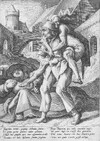
\includegraphics[keepaspectratio,width=\textwidth]{carrying-povery-small.jpg}
  \captionart{PovertyRiches}
  \label{fig:povertyriches}
\end{figure}

% Force float here
\clearpage{}
\thispagestyle{titleontop}
%SECT. II. MEMB. IV SUBSECT. VI.-_Poverty and Want, Causes of Melancholy_.
\section{Poverty and Want, Causes of Melancholy.}\label{sec:poverty-and-want}

\lettrine{P}{overty} and want are so violent oppugners, so unwelcome guests, so much
abhorred of all men, that I may not omit to speak of them apart.
Poverty, although (if considered aright, to a wise, understanding,
truly regenerate, and contented man) it be donum Dei, a blessed estate,
the way to heaven, as \Chrysostom{} calls\authorfootnote{2203} it, God's gift, the mother
of modesty, and much to be preferred before riches (as shall be shown
in his \authorfootnote{2204}place), yet as it is esteemed in the world's censure, it
is a most odious calling, vile and base, a severe torture, summum
scelus, a most intolerable burden; we \authorfootnote{2205}shun it all, cane pejus et
angue (worse than a dog or a snake), we abhor the name of it,
\authorfootnote{2206}Paupertas fugitur, totoque arcessitur orbe, as being the fountain
of all other miseries, cares, woes, labours, and grievances whatsoever.
To avoid which, we will take any pains,-extremos currit mercator ad
Indos, we will leave no haven, no coast, no creek of the world
unsearched, though it be to the hazard of our lives, we will dive to
the bottom of the sea, to the bowels of the earth, \authormarginnote{2207}five, six,
seven, eight, nine hundred fathom deep, through all five zones, and
both extremes of heat and cold: we will turn parasites and slaves,
prostitute ourselves, swear and lie, damn our bodies and souls, forsake
God, abjure religion, steal, rob, murder, rather than endure this
insufferable yoke of poverty, which doth so tyrannise, crucify, and
generally depress us.

For look into the world, and you shall see men most part esteemed
according to their means, and happy as they are rich: \li{Ubique
tanti quisque quantum habuit fuit.}\authormarginnote{2208} If he be likely to thrive, and in
the way of preferment, who but he? In the vulgar opinion, if a man be
wealthy, no matter how he gets it, of what parentage, how qualified,
how virtuously endowed, or villainously inclined; let him be a bawd, a
gripe, an usurer, a villain, a pagan, a barbarian, a wretch,
\authorfootnote{2209}Lucian's tyrant, on whom you may look with less security than on
the sun; so that he be rich (and liberal withal) he shall be honoured,
admired, adored, reverenced, and highly \authorfootnote{2210}magnified. The rich is
had in reputation because of his goods, Eccl. \rn{x}. 31. He shall be
befriended: for riches gather many friends, Prov. \rn{xix.} 4,-\lit{all happiness ebbs and flows with his money}{multos numerabit amicos}\authormarginnote{2211}. He
shall be accounted a gracious lord, a Mecaenas, a benefactor, a wise,
discreet, a proper, a valiant, a fortunate man, of a generous spirit,
\li{Pullus Jovis, et gallinae, filius albae}: a hopeful, a good man, a
virtuous, honest man. \li{Quando ego ie Junonium puerum, et matris partum
vere aureum}, as Tully said\authorfootnote{2212} of Octavianus, while he was adopted
Caesar, and an heir apparent of so great a monarchy\authormarginnote{2213}, he was a
golden child. All \authorfootnote{2214}honour, offices, applause, grand titles, and
turgent epithets are put upon him, omnes omnia bona dicere; all men's
eyes are upon him, God bless his good worship, his honour; \authorfootnote{2215}every
man speaks well of him, every man presents him, seeks and sues to him
for his love, favour, and protection, to serve him, belong unto him,
every man riseth to him, as to Themistocles in the Olympics, if he
speak, as of Herod, Vox Dei, non hominis, the voice of God, not of man.
All the graces, Veneres, pleasures, elegances attend him, \authorfootnote{2216} golden
fortune accompanies and lodgeth with him; and as to those Roman
emperors, is placed in his chamber.
\authorfootnote{2217}---Secura naviget aura,
Fortunamque suo temperet arbitrio:

he may sail as he will himself, and temper his estate at his pleasure,
jovial days, splendour and magnificence, sweet music, dainty fare, the
good things, and fat of the land, fine clothes, rich attires, soft
beds, down pillows are at his command, all the world labours for him,
thousands of artificers are his slaves to drudge for him, run, ride,
and post for him: \authorfootnote{2218}Divines (for Pythia Philippisat) lawyers,
physicians, philosophers, scholars are his, wholly devote to his
service. Every man seeks his \authorfootnote{2219}acquaintance, his kindred, to match
with him, though he be an oaf, a ninny, a monster, a goose-cap, \li{uxorem
ducat Danaen}\authorlatintrans{2220}, when, and whom he will, hunc optant generum Rex et
Regina-he is an excellent \authorfootnote{2221}match for my son, my daughter, my
niece, \etc{}. Quicquid calcaverit hic, Rosa fiet, let him go whither he
will, trumpets sound, bells ring, \etc{}, all happiness attends him, every
man is willing to entertain him, he sups in \authorfootnote{2222}Apollo wheresoever he
comes; what preparation is made for his \authorfootnote{2223}entertainment? fish and
fowl, spices and perfumes, all that sea and land affords. What cookery,
masking, mirth to exhilarate his person?
\authorfootnote{2224}Da Trebio, pone ad Trebium, vis frater ab illia
Ilibus?---

What dish will your good worship eat of?
\authorfootnote{2225}---dulcia poma,
Et quoscunque feret cultus tibi fundus honores,
Ante Larem, gustet venerabilior Lare dives.

Sweet apples, and whate'er thy fields afford,
Before thy Gods be serv'd, let serve thy Lord.

What sport will your honour have? hawking, hunting, fishing, fowling,
bulls, bears, cards, dice, cocks, players, tumblers, fiddlers, jesters,
\etc{}, they are at your good worship's command. Fair houses, gardens,
orchards, terraces, galleries, cabinets, pleasant walks, delightsome
places, they are at hand: \authorfootnote{2226}in aureis lac, vinum in argenteis,
adolescentulae ad nutum speciosae, wine, wenches, \etc{} a Turkish
paradise, a heaven upon earth. Though he be a silly soft fellow, and
scarce have common sense, yet if he be borne to fortunes (as I have
said) \authorfootnote{2227}jure haereditario sapere jubetur, he must have honour and
office in his course: \authorfootnote{2228}Nemo nisi dives honore dignus (Ambros.
offic. 21.) none so worthy as himself: he shall have it, atque esto
quicquid Servius aut Labeo. Get money enough and command
\authorfootnote{2229}kingdoms, provinces, armies, hearts, hands, and affections; thou
shalt have popes, patriarchs to be thy chaplains and parasites: thou
shalt have (Tamerlane-like) kings to draw thy coach, queens to be thy
laundresses, emperors thy footstools, build more towns and cities than
great Alexander, Babel towers, pyramids and Mausolean tombs, \etc{}
command heaven and earth, and tell the world it is thy vassal, \li{auro
emitur diadema, argento caelum panditur, denarius philosophum conducit,
nummus jus cogit, obolus literatum pascit, metallum sanitatem
conciliat, aes amicos conglutinat}\authorlatintrans{2230}. And therefore not without good
cause, John de Medicis, that rich Florentine, when he lay upon his
death-bed, calling his sons, Cosmo and Laurence, before him, amongst
other sober sayings, repeated this, animo quieto digredior, quod vos
sanos et divites post me relinquam, It doth me good to think yet,
though I be dying, that I shall leave you, my children, sound and rich:
for wealth sways all. It is not with us, as amongst those Lacedaemonian
senators of Lycurgus in Plutarch, He preferred that deserved best, was
most virtuous and worthy of the place, \authorfootnote{2231}not swiftness, or
strength, or wealth, or friends carried it in those days: but inter
optimos optimus, inter temperantes temperantissimus, the most temperate
and best. We have no aristocracies but in contemplation, all
oligarchies, wherein a few rich men domineer, do what they list, and
are privileged by their greatness. \authorfootnote{2232}They may freely trespass, and
do as they please, no man dare accuse them, no not so much as mutter
against them, there is no notice taken of it, they may securely do it,
live after their own laws, and for their money get pardons,
indulgences, redeem their souls from purgatory and hell itself,-\li{clausum
possidet arca Jovem}. Let them be epicures, or atheists, libertines,
Machiavellians, (as they often are) \authorfootnote{2233}\li{Et quamvis perjuris erit},
sine gente, cruentus, they may go to heaven through the eye of a
needle, if they will themselves, they may be canonised for saints, they
shall be \authorfootnote{2234}honourably interred in Mausolean tombs, commended by
poets, registered in histories, have temples and statues erected to
their names,-\li{e manibus illis-nascentur violae.}-If he be bountiful in
his life, and liberal at his death, he shall have one to swear, as he
did by Claudius the Emperor in Tacitus, he saw his soul go to heaven,
and be miserably lamented at his funeral. \li{Ambubalarum collegia, \etc{}.
Trimalcionis topanta in Petronius recta in caelum abiit}, went right to
heaven: a, base quean, \authorfootnote{2235}thou wouldst have scorned once in thy
misery to have a penny from her; and why? \li{modio nummos metiit}, she
measured her money by the bushel. These prerogatives do not usually
belong to rich men, but to such as are most part seeming rich, let him
have but a good outside\authormarginnote{2236}, he carries it, and shall be adored for a
god, as Cyrus was\authorfootnote{2237} amongst the Persians, \lit{for his gay attires}{ob splendidum apparatum}
; now most men are esteemed according to their
clothes. In our gullish times, whom you peradventure in modesty would
give place to, as being deceived by his habit, and presuming him some
great worshipful man, believe it, if you shall examine his estate, he
will likely be proved a serving man of no great note, my lady's tailor,
his lordship's barber, or some such gull, a Fastidius Brisk, Sir
Petronel Flash, a mere outside. Only this respect is given him, that
wheresoever he comes, he may call for what he will, and take place by
reason of his outward habit.

But on the contrary, if he be poor, Prov. \rn{xv.} 15, all his days are
miserable, he is under hatches, dejected, rejected and forsaken, poor
in purse, poor in spirit; \authorfootnote{2238}prout res nobis fluit, ita et animus se
habet; \authorfootnote{2239}money gives life and soul. Though he be honest, wise,
learned, well-deserving, noble by birth, and of excellent good parts;
yet in that he is poor, unlikely to rise, come to honour, office, or
good means, he is contemned, neglected, \li{frustra sapit, inter literas
esurit, amicus molestus}. \authorfootnote{2240}If he speak, what babbler is this?
Ecclus, his nobility without wealth, is \li{projecta vilior alga}\authorlatintrans{2241.5}\authormarginnote{2241}, and
he not esteemed: nos viles pulli nati infelicibus ovis, if once poor,
we are metamorphosed in an instant, base slaves, villains, and vile
drudges; \authorfootnote{2242}for to be poor, is to be a knave, a fool, a wretch, a
wicked, an odious fellow, a common eyesore, say poor and say all; they
are born to labour, to misery, to carry burdens like juments, pistum
stercus comedere with Ulysses' companions, and as Chremilus objected in
Aristophanes, \authorfootnote{2243} salem lingere, lick salt, to empty jakes, fay
channels, \authorfootnote{2244}carry out dirt and dunghills, sweep chimneys, rub
horse-heels, \etc{}. I say nothing of Turks, galley-slaves, which are
bought \authorfootnote{2245}and sold like juments, or those African Negroes, or poor
\authorfootnote{2246}Indian drudges, \li{qui indies hinc inde deferendis oneribus
occumbunt, nam quod apud nos boves et asini vehunt, trahunt, \etc{}}\authorlatintrans{2247}.
\li{Id omne misellis Indis}, they are ugly to behold, and though erst
spruce, now rusty and squalid, because poor, \authorfootnote{2248}\li{immundas fortunas
aquum est squalorem sequi}, it is ordinarily so. \authorfootnote{2249}Others eat to
live, but they live to drudge, \authorfootnote{2250}\li{servilis et misera gens nihil
recusare audet}, a servile generation, that dare refuse no
task.-\authorfootnote{2251}\li{Heus tu Dromo, cape hoc flabellum, ventulum hinc facito dum
lavamus}, sirrah blow wind upon us while we wash, and bid your fellow
get him up betimes in the morning, be it fair or foul, he shall run
fifty miles afoot tomorrow, to carry me a letter to my mistress, Socia
ad pistrinam, Socia shall tarry at home and grind malt all day long,
Tristan thresh. Thus are they commanded, being indeed some of them as
so many footstools for rich men to tread on, blocks for them to get on
horseback, or as walls for them to piss on\authorfootnote{2252}. They are commonly
such people, rude, silly, superstitious idiots, nasty, unclean, lousy,
poor, dejected, slavishly humble: and as Leo Afer observes\authorfootnote{2253} of the
commonalty of Africa, \li{natura viliores sunt, nec apud suos duces majore
in precio quam si canes essent}: \authorfootnote{2254}base by nature, and no more
esteemed than dogs, \li{miseram, laboriosam, calamitosam vitam agunt, et
inopem, infelicem, rudiores asinis, ut e brutis plane natos dicas}: no
learning, no knowledge, no civility, scarce common, sense, nought but
barbarism amongst them, \li{belluino more vivunt, neque calceos gestant,
neque vestes}, like rogues and vagabonds, they go barefooted and
barelegged, the soles of their feet being as hard as horse-hoofs, as
\authorfootnote{2255}Radzivilus observed at Damietta in Egypt, leading a laborious,
miserable, wretched, unhappy life, \authorfootnote{2256}like beasts and juments, if
not worse: (for a \authorfootnote{2257}Spaniard in Incatan, sold three Indian boys for
a cheese, and a hundred Negro slaves for a horse) their discourse is
scurrility, their summum bonum, a pot of ale. There is not any slavery
which these villains will not undergo, inter illos plerique latrinas
evacuant, alii culinariam curant, alii stabularios agunt, urinatores et
id genus similia exercent, \etc{} like those people that dwell in the
\authorfootnote{2258}Alps, chimney-sweepers, jakes-farmers, dirt-daubers, vagrant
rogues, they labour hard some, and yet cannot get clothes to put on, or
bread to eat. For what can filthy poverty give else, but beggary,
fulsome nastiness, squalor, contempt, drudgery, labour, ugliness,
hunger and thirst\authormarginnote{2259}; \li{pediculorum, et pulicum numerum?} as he well
followed\authorfootnote{2260} it in Aristophanes, fleas and lice, \li{pro pallio vestem laceram,
et pro pulvinari lapidem bene magnum ad caput}, rags for his raiment,
and a stone for his pillow, \li{pro cathedra, ruptae caput urnae}, he sits
in a broken pitcher, or on a block for a chair, \li{et malvae, ramos pro
panibus comedit}, he drinks water, and lives on wort leaves, pulse, like
a hog, or scraps like a dog, \li{ut nunc nobis vita afficitur, quis non
putabit insaniam esse, infelicitatemque?} as Chremilus concludes his
speech, as we poor men live nowadays, who will not take our life to be
\authorfootnote{2261} infelicity, misery, and madness?

If they be of little better condition than those base villains,
hunger-starved beggars, wandering rogues, those ordinary slaves, and
day-labouring drudges; yet they are commonly so preyed upon by \authorfootnote{2262}
polling officers for breaking the laws, by their tyrannising landlords,
so flayed and fleeced by perpetual \authorfootnote{2263}exactions, that though they do
drudge, fare hard, and starve their genius, they cannot live in
\authorfootnote{2264}some countries; but what they have is instantly taken from them,
the very care they take to live, to be drudges, to maintain their poor
families, their trouble and anxiety takes away their sleep, Sirac.
\rn{xxxi.} 1, it makes them weary of their lives: when they have taken all
pains, done their utmost and honest endeavours, if they be cast behind
by sickness, or overtaken with years, no man pities them, hard-hearted
and merciless, uncharitable as they are, they leave them so distressed,
to beg, steal, murmur, and \authormarginnote{2265} rebel, or else starve. The feeling
and fear of this misery compelled those old Romans, whom Menenius
Agrippa pacified, to resist their governors: outlaws, and rebels in
most places, to take up seditious arms, and in all ages hath caused
uproars, murmurings, seditions, rebellions, thefts, murders, mutinies,
jars and contentions in every commonwealth: grudging, repining,
complaining, discontent in each private family, because they want means
to live according to their callings, bring up their children, it breaks
their hearts, they cannot do as they would. No greater misery than for
a lord to have a knight's living, a gentleman a yeoman's, not to be
able to live as his birth and place require. Poverty and want are
generally corrosives to all kinds of men, especially to such as have
been in good and flourishing estate, are suddenly distressed,
\authorfootnote{2266}nobly born, liberally brought up, and, by some disaster and
casualty miserably dejected. For the rest, as they have base fortunes,
so have they base minds correspondent, like beetles, e stercore orti, e
stercore victus, in stercore delicium, as they were obscurely born and
bred, so they delight in obscenity; they are not thoroughly touched
with it. \li{Angustas animas angusto in pectore versant}\authorlatintrans{2267}. Yet, that
which is no small cause of their torments, if once they come to be in
distress, they are forsaken of their fellows, most part neglected, and
left unto themselves; as poor \authorfootnote{2268}Terence in Rome was by Scipio,
Laelius, and Furius, his great and noble friends.
%
\begin{latin}
\begin{quote}
Nil Publius Scipio profuit, nil ei Laelius, nil Furius,\\
Tres per idem tempus qui agitabant nobiles facillime,\\
Horum ille opera ne domum quident habuit conductitiam.
\end{quote}
\end{latin}
\translationrule
\begin{quote}%\authorlatintrans{2269}
Publius Scipio, Laelius and Furius, three of the most distinguished noblemen at that day in Rome, were of so little service to him, that he could scarcely procure a lodging through their patronage.
\end{quote}

'Tis generally so, \li{Tempora si fuerint nubila, solus eris}, he is left
cold and comfortless, \li{nullas ad amissas ibit amicus opes}, all flee from
him as from a rotten wall, now ready to fall on their heads. Prov. \rn{xix.}
1. Poverty separates them from their \authormarginnote{2270}neighbours.
\li{Dum fortuna favet vultum servatis amici,
Cum cecidit, turpi vertitis ora fuga.}\authormarginnote{2271}

Whilst fortune favour'd, friends, you smil'd on me,
But when she fled, a friend I could not see.

Which is worse yet, if he be poor \authorfootnote{2272}every man contemns him, insults
over him, oppresseth him, scoffs at, aggravates his misery.
\li{Quum caepit quassata domus subsidere, partes
In proclinatas omne recumbit onus.}\authormarginnote{2273}

When once the tottering house begins to shrink,
Thither comes all the weight by an instinct.

Nay they are odious to their own brethren, and dearest friends, Pro.
xix. 7. His brethren hate him if he be poor, \authorfootnote{2274}omnes vicini
oderunt, his neighbours hate him, Pro. xiv. 20, \authorfootnote{2275}omnes me noti ac
ignoti deserunt, as he complained in the comedy, friends and strangers,
all forsake me. Which is most grievous, poverty makes men ridiculous,
Nil habet infelix paupertas durius in se, quam quod ridiculos homines
facit, they must endure \authorfootnote{2276}jests, taunts, flouts, blows of their
betters, and take all in good part to get a meal's meat: \authorfootnote{2277}magnum
pauperies opprobrium, jubet quidvis et facere et pati. He must turn
parasite, jester, fool, cum desipientibus desipere; saith
\authorfootnote{2278}Euripides, slave, villain, drudge to get a poor living, apply
himself to each man's humours, to win and please, \etc{}, and be buffeted
when he hath all done, as Ulysses was by Melanthius \authorfootnote{2279}in Homer, be
reviled, baffled, insulted over, for \authorfootnote{2280}potentiorum stultitia
perferenda est, and may not so much as mutter against it. He must turn
rogue and villain; for as the saying is, \li{Necessitas cogit ad turpia},
poverty alone makes men thieves, rebels, murderers, traitors,
assassins, because of poverty we have sinned, Ecclus. \rn{xxvii.} 1, swear
and forswear, bear false witness, lie, dissemble, anything, as I say,
to advantage themselves, and to relieve their necessities: \authorfootnote{2281}
Culpae scelerisque magistra est, when a man is driven to his shifts,
what will he not do?

---\li{si miserum fortuna Sinonem
Finxit, vanum etiam mendacemque improba finget}\authorlatintrans{2282}.

he will betray his father, prince, and country, turn Turk, forsake
religion, abjure God and all, nulla tam horrenda proditio, quam illi
lucri causa (saith \authorfootnote{2283}Leo Afer) perpetrare nolint. \authorfootnote{2284}Plato,
therefore, calls poverty, thievish, sacrilegious, filthy, wicked, and
mischievous: and well he might. For it makes many an upright man
otherwise, had he not been in want, to take bribes, to be corrupt, to
do against his conscience, to sell his tongue, heart, hand, \etc{}, to be
churlish, hard, unmerciful, uncivil, to use indirect means to help his
present estate. It makes princes to exact upon their subjects, great
men tyrannise, landlords oppress, justice mercenary, lawyers vultures,
physicians harpies, friends importunate, tradesmen liars, honest men
thieves, devout assassins, great men to prostitute their wives,
daughters, and themselves, middle sort to repine, commons to mutiny,
all to grudge, murmur, and complain. A great temptation to all
mischief, it compels some miserable wretches to counterfeit several
diseases, to dismember, make themselves blind, lame, to have a more
plausible cause to beg, and lose their limbs to recover their present
wants. Jodocus Damhoderius, a lawyer of Bruges, praxi rerum criminal.
c. 112. hath some notable examples of such counterfeit cranks, and
every village almost will yield abundant testimonies amongst us; we
have dummerers, Abraham men, \etc{}. And that which is the extent of
misery, it enforceth them through anguish and wearisomeness of their
lives, to make away themselves; they had rather be hanged, drowned,
\etc{}, than to live without means.
\authorfootnote{2285}In mare caetiferum, ne te premat aspera egestas,
Desili, et a celsis corrue Cerne jugis.


Much better 'tis to break thy neck,
Or drown thyself i' the sea,

Than suffer irksome poverty;
Go make thyself away.

A Sybarite of old, as I find it registered in \authorfootnote{2286}Athenaeus, supping
in Phiditiis in Sparta, and observing their hard fare, said it was no
marvel if the Lacedaemonians were valiant men; for his part, he would
rather run upon a sword point (and so would any man in his wits) than
live with such base diet, or lead so wretched a life. \authorfootnote{2287}In Japonia,
'tis a common thing to stifle their children if they be poor, or to
make an abortion, which \Aristotle commends. In that civil commonwealth
of China, \authorfootnote{2288}the mother strangles her child, if she be not able to
bring it up, and had rather lose, than sell it, or have it endure such
misery as poor men do. Arnobius, lib. 7, adversus gentes,
\authorfootnote{2289}Lactantius, lib. 5. cap. 9. objects as much to those ancient
Greeks and Romans, they did expose their children to wild beasts,
strangle, or knock out their brains against a stone, in such cases. If
we may give credit to \authorfootnote{2290}Munster, amongst us Christians in
Lithuania, they voluntarily mancipate and sell themselves, their wives
and children to rich men, to avoid hunger and beggary; \authorfootnote{2291} many make
away themselves in this extremity. Apicius the Roman, when he cast up
his accounts, and found but 100\thinspace{}000 crowns left, murdered himself for
fear he should be famished to death. P. Forestus, in his medicinal
observations, hath a memorable example of two brothers of Louvain that,
being destitute of means, became both melancholy, and in a discontented
humour massacred themselves. Another of a merchant, learned, wise
otherwise and discreet, but out of a deep apprehension he had of a loss
at seas, would not be persuaded but as Ventidius\authorfootnote{2292} in the poet, he
should die a beggar. In a word, thus much I may conclude of poor men,
that though they have good \authorfootnote{2293}parts they cannot show or make use of
them: \authorfootnote{2294}ab inopia ad virtutem obsepta est via, 'tis hard for a poor
man to \authorfootnote{2295} rise, \li{haud facile emergunt, quorum virtutibus obstat res
angusta domi}\authorlatintrans{2296}. The wisdom of the poor is despised, and his words
are not heard. Eccles. \rn{vi.} 19. His works are rejected, contemned, for
the baseness and obscurity of the author, though laudable and good in
themselves, they will not likely take.
Nulla placere diu, neque vivere carmina possunt,
Quae scribuntur atquae potoribus.---

No verses can please men or live long that are written by
water-drinkers. Poor men cannot please, their actions, counsels,
consultations, projects, are vilified in the world's esteem, amittunt
consilium in re, which Gnatho long since observed. \authorfootnote{2297}Sapiens
crepidas sibi nunquam nec soleas fecit, a wise man never cobbled shoes;
as he said of old, but how doth he prove it? I am sure we find it
otherwise in our days, \authorfootnote{2298} pruinosis horret facundia pannis. Homer
himself must beg if he want means, and as by report sometimes he did
\authorfootnote{2299}go from door to door, and sing ballads, with a company of boys
about him. This common misery of theirs must needs distract, make them
discontent and melancholy, as ordinarily they are, wayward, peevish,
like a weary traveller, for \authorfootnote{2300} Fames et mora bilem in nares
conciunt, still murmuring and repining: Ob inopiam morosi sunt, quibus
est male, as Plutarch quotes out of Euripides, and that comical poet
well seconds,\authorfootnote{2301}

\begin{latin}
\begin{quote}
Omnes quibus res sunt minus secundae, nescio quomodo
Suspitiosi, ad contumeliam omnia accipiunt magis,
Propter suam impotentiam se credunt negligi.
\end{quote}
\end{latin}

If they be in adversity, they are more suspicious and apt to mistake:
they think themselves scorned by reason of their misery: and therefore
many generous spirits in such cases withdraw themselves from all
company, as that comedian Terence is said\authormarginnote{2302} to have done; when he
perceived himself to be forsaken and poor, he voluntarily banished
himself to Stymphalus, a base town in Arcadia, and there miserably
died.
%
\begin{latin}
\begin{quote}
---ad summam inopiam redactus,\\
Itaque e conspectu omnium abiit Graeciae in terram ultimam.
\end{quote}
\end{latin}
\translationrule
\begin{quote}%\authorlatintrans{2303}.
Reduced to the greatest necessity, he withdrew from the gaze of the public to the most remote village in Greece.
\end{quote}

Neither is it without cause, for we see men commonly respected
according to their means, (\li{an dives sit omnes quaerunt, nemo an
bonus}\authormarginnote{2304}) and vilified if they be in bad clothes. \authorfootnote{2305}Philophaemen the
orator was set to cut wood, because he was so homely attired,
\authorfootnote{2306}Terentius was placed at the lower end of Cecilius' table, because
of his homely outside. \authorfootnote{2307} Dante, that famous Italian poet, by
reason his clothes were but mean, could not be admitted to sit down at
a feast. Gnatho scorned his old familiar friend because of his apparel,
\authorfootnote{2308}Hominem video pannis, annisque obsitum, hic ego illum contempsi
prae me. King Persius overcome sent a letter to \authorfootnote{2309}Paulus Aemilius,
the Roman general; Persius P. Consuli. S. but he scorned him any
answer, tacite exprobrans fortunam suam (saith mine author) upbraiding
him with a present fortune. \authorfootnote{2310}Carolus Pugnax, that great duke of
Burgundy, made H. Holland, late duke of Exeter, exiled, run after his
horse like a lackey, and would take no notice of him: \authormarginnote{2311} 'tis the
common fashion of the world. So that such men as are poor may justly be
discontent, melancholy, and complain of their present misery, and all
may pray with \authorfootnote{2312}Solomon, Give me, O Lord, neither riches nor
poverty; feed me with food convenient for me.

%SECT. II. MEMB. IV. SUBSECT. VII.-_A heap of other Accidents causing Melancholy, Death of Friends, Losses, \etc{}._
\section[Accidents, Death of Friends, Losses]{A heap of other Accidents causing Melancholy, Death of Friends, Losses, \etc{}}\label{sec:accidents-death-of-friends}

\lettrine{I}{n} this labyrinth of accidental causes, the farther I wander, the more
intricate I find the passage, multae ambages, and new causes as so many
by-paths offer themselves to be discussed: to search out all, were an
Herculean work, and fitter for Theseus: I will follow mine intended
thread; and point only at some few of the chiefest.
\subsection{Death of Friends.}
Amongst which, loss and death of friends may
challenge a first place, multi tristantur, as Vives well
observes\authorfootnote{2313}, post delicias, convivia, dies festos, many are melancholy
after a feast, holiday, merry meeting, or some pleasing sport, if they
be solitary by chance, left alone to themselves, without employment,
sport, or want their ordinary companions, some at the departure of
friends only whom they shall shortly see again, weep and howl, and look
after them as a cow lows after her calf, or a child takes on that goes
to school after holidays. Ut me levarat tuus adventus, sic discessus
afflixit, (which \authorfootnote{2314}Tully writ to Atticus) thy coming was not so
welcome to me, as thy departure was harsh. Montanus, consil. 132. makes
mention of a country woman that parting with her friends and native
place, became grievously melancholy for many years; and Trallianus of
another, so caused for the absence of her husband: which is an ordinary
passion amongst our good wives, if their husband tarry out a day longer
than his appointed time, or break his hour, they take on presently with
sighs and tears, he is either robbed, or dead, some mischance or other
is surely befallen him, they cannot eat, drink, sleep, or be quiet in
mind, till they see him again. If parting of friends, absence alone can
work such violent effects, what shall death do, when they must
eternally be separated, never in this world to meet again? This is so
grievous a torment for the time, that it takes away their appetite,
desire of life, extinguisheth all delights, it causeth deep sighs and
groans, tears, exclamations,
(\li{O dulce germen matris, o sanguis meus, Eheu tepentes, \etc{}-o flos tener}\authorlatintrans{2315}.) 
howling, roaring, many bitter pangs, \authormarginnote{2316}\li{lamentis gemituque et
faemineo ululatu Tecta fremunt}) and by frequent meditation extends so
far sometimes, \authorfootnote{2317}they think they see their dead friends continually
in their eyes, observantes imagines, as Conciliator confesseth he saw
his mother's ghost presenting herself still before him. Quod nimis
miseri volunt, hoc facile credunt, still, still, still, that good
father, that good son, that good wife, that dear friend runs in their
minds: Totus animus hac una cogitatione defixus est, all the year long,
as \Pliny{} complains\authorfootnote{2318} to Romanus, methinks I see Virginius, I hear
Virginius, I talk with Virginius, \etc{}.
%
\authormarginnote{2319}\begin{latin}
\begin{verse}
Te sine, vae misero mihi, lilia nigra videntur,\\*
Pallentesque rosae, nec dulce rubens hyacinthus,\\*
Nullos nec myrtus, noc laurus spirat odores.
\end{verse}
\end{latin}
\translationrule
\begin{verse}% \authorlatintrans{2319.5}
Without thee, ah! wretched me,\\*
the lillies lose their whiteness, the roses become pallid, the hyacinth forgets to blush\\*
neither the myrtle nor the laurel retains its odours.
\end{verse}

\cleartoleftpage{}
\begin{figure}[p]
  \begingroup
  \centering
  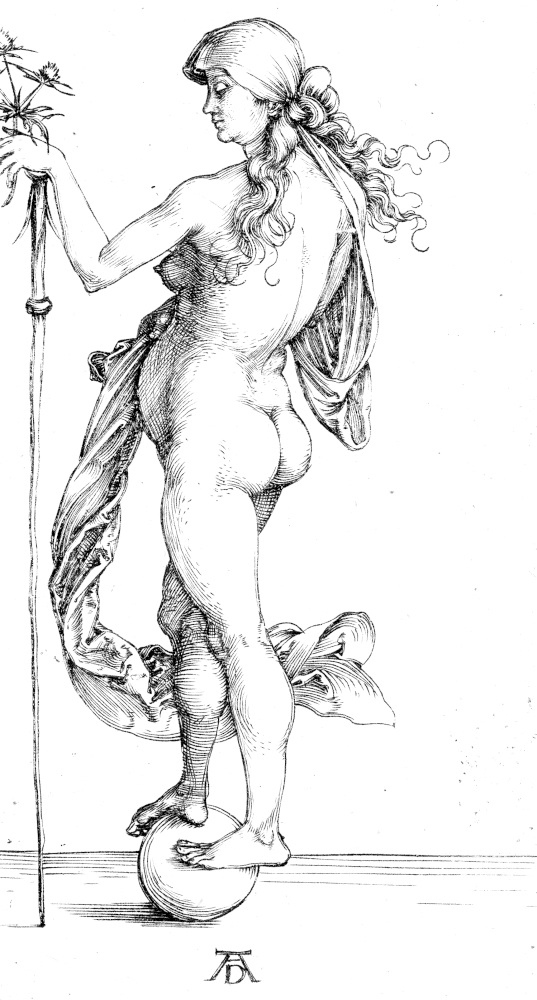
\includegraphics[keepaspectratio,width=0.75\textwidth]{fortuna-small.jpg}
  \captionart{Fortuna}
  \label{fig:fortuna}
\end{figure}

% Force float here
\clearpage{}
They that are most staid and patient, are so furiously carried headlong
by the passion of sorrow in this case, that brave discreet men
otherwise, oftentimes forget themselves, and weep like children many
months together, \authorfootnote{2320}as if that they to water would, and will not be
comforted. They are gone, they are gone; what shall I do?
Abstulit atra dies et funere mersit acerbo,
Quis dabit in lachrymas fontem mihi? quis satis altos
Accendet gemitus, et acerbo verba dolori?
Exhaurit pietas oculos, et hiantia frangit
Pectora, nec plenos avido sinit edere questus,
Magna adeo jactura premit, \etc{}.

Fountains of tears who gives, who lends me groans,
Deep sighs sufficient to express my moans?
Mine eyes are dry, my breast in pieces torn,
My loss so great, I cannot enough mourn.

So Stroza Filius, that elegant Italian poet, in his Epicedium, bewails
his father's death, he could moderate his passions in other matters,
(as he confesseth) but not in this, lie yields wholly to sorrow,
Nunc fateor do terga malis, mens illa fatiscit,
Indomitus quondam vigor et constantia mentis.

How doth \authorfootnote{2321}Quintilian complain for the loss of his son, to despair
almost: Cardan lament his only child in his book de libris propriis,
and elsewhere in many of his tracts, \authorfootnote{2322}St. Ambrose his brother's
death? an ego possum non cogitare de te, aut sine lachrymis cogitare? O
amari dies, o flebiles noctes, \etc{}. Can I ever cease to think of thee,
and to think with sorrow? O bitter days, O nights of sorrow, \etc{}.
Gregory Nazianzen, that noble Pulcheria! O decorem, \etc{} flos recens,
pullulans, \etc{}. Alexander, a man of most invincible courage, after
Hephestion's death, as Curtius relates, triduum jacuit ad moriendum
obstinatus, lay three days together upon the ground, obstinate, to die
with him, and would neither eat, drink, nor sleep. The woman that
communed with Esdras (lib. 2. cap. 10.) when her son fell down dead.
fled into the field, and would not return into the city, but there
resolved to remain, neither to eat nor drink, but mourn and fast until
she died. Rachel wept for her children, and would not be comforted
because they were not. Matt. ii. 18. So did Adrian the emperor bewail
his Antinous; Hercules, Hylas; Orpheus, Eurydice; David, Absalom; (O my
dear son Absalom) \Austin{} his mother Monica, Niobe her children,
insomuch that the \authorfootnote{2323}poets feigned her to be turned into a stone, as
being stupefied through the extremity of grief. \authorfootnote{2324}Aegeas, signo
lugubri filii consternatus, in mare se proecipitatem dedit, impatient
of sorrow for his son's death, drowned, himself. Our late physicians
are full of such examples. Montanus consil. 242. \authorfootnote{2325}had a patient
troubled with this infirmity, by reason of her husband's death, many
years together. Trincavellius, l. 1. c. 14. hath such another, almost
in despair, after his \authorfootnote{2326}mother's departure, ut se ferme
proecipitatem daret; and ready through distraction to make away
himself: and in his Fifteenth counsel, tells a story of one fifty years
of age, that grew desperate upon his mother's death; and cured by
Fallopius, fell many years after into a relapse, by the sudden death of
a daughter which he had, and could never after be recovered. The fury
of this passion is so violent sometimes, that it daunts whole kingdoms
and cities. Vespasian's death was pitifully lamented all over the Roman
empire, totus orbis lugebat, saith Aurelius Victor. Alexander commanded
the battlements of houses to be pulled down, mules and horses to have
their manes shorn off, and many common soldiers to be slain, to
accompany his dear Hephestion's death; which is now practised amongst
the Tartars, when \authorfootnote{2327}a great Cham dieth, ten or twelve thousand must
be slain, men and horses, all they meet; and among those the
\authorfootnote{2328}Pagan Indians, their wives and servants voluntarily die with
them. Leo Decimus was so much bewailed in Rome after his departure,
that as Jovius gives out, \authorfootnote{2329}communis salus, publica hilaritas, the
common safety of all good fellowship, peace, mirth, and plenty died
with him, tanquam eodem sepulchro cum Leone condita lugebantur: for it
was a golden age whilst he lived, \authorfootnote{2330}but after his decease an iron
season succeeded, barbara vis et foeda vastitas, et dira malorum omnium
incommoda, wars, plagues, vastity, discontent. When Augustus Caesar
died, saith Paterculus, orbis ruinam timueramus, we were all afraid, as
if heaven had fallen upon our heads. \authorfootnote{2331}Budaeus records, how that,
at Lewis the Twelfth his death, tam subita mutatio, ut qui prius digito
coelum attingere videbantur, nunc humi derepente serpere, sideratos
esse diceres, they that were erst in heaven, upon a sudden, as if they
had been planet-strucken, lay grovelling on the ground;
\li{Concussis cecidere animis, seu frondibus ingens
Sylva dolet lapsis}\authorlatintrans{2332.5}---\authormarginnote{2332}

they looked like cropped trees. \authorfootnote{2333}At Nancy in Lorraine, when
Claudia Valesia, Henry the Second French king's sister, and the duke's
wife deceased, the temples for forty days were all shut up, no prayers
nor masses, but in that room where she was. The senators all seen in
black, and for a twelvemonth's space throughout the city, they were
forbid to sing or dance.
\authorfootnote{2334}Non ulli pastos illis egre diebus
Frigida (Daphne) boves ad flumina, nulla nec amnem
Libavit quadrupes, nec graminis attigit herbam.

The swains forgot their sheep, nor near the brink
Of running waters brought their herds to drink;
The thirsty cattle, of themselves, abstained
From water, and their grassy fare disdain'd.

How were we affected here in England for our Titus, deliciae, humani
generis, Prince Henry's immature death, as if all our dearest friends'
lives had exhaled with his? \authorfootnote{2335}Scanderbeg's death was not so much
lamented in Epirus. In a word, as he saith\authorfootnote{2336} of Edward the First at
the news of Edward of Caernarvon his son's birth, immortaliter gavisus,
he was immortally glad, may we say on the contrary of friends' deaths,
immortaliter gementes, we are diverse of us as so many turtles,
eternally dejected with it.
There is another sorrow, which arises from the loss of temporal goods
and fortunes, which equally afflicts, and may go hand in hand with the
preceding; loss of time, loss of honour, office, of good name, of
labour, frustrate hopes, will much torment; but in my judgment, there
is no torture like unto it, or that sooner procureth this malady and
mischief:
\authorfootnote{2337}Ploratur lachrymis amissa pecunia veris:

Lost money is bewailed with grief sincere.

it wrings true tears from our eyes, many sighs, much sorrow from our
hearts, and often causes habitual melancholy itself, Guianerius tract.
15. 5. repeats this for an especial cause: \authorfootnote{2338}Loss of friends, and
loss of goods, make many men melancholy, as I have often seen by
continual meditation of such things. The same causes Arnoldus
Villanovanus inculcates, Breviar. l. 1. c. 18. ex rerum amissione,
damno, amicorum morte, \etc{}. Want alone will make a man mad, to be Sans
argent will cause a deep and grievous melancholy. Many persons are
affected like \authorfootnote{2339} Irishmen in this behalf, who if they have a good
scimitar, had rather have a blow on their arm, than their weapon hurt:
they will sooner lose their life, than their goods: and the grief that
cometh hence, continueth long (saith \authorfootnote{2340}Plater) and out of many
dispositions, procureth an habit. \authorfootnote{2341}Montanus and Frisemelica cured
a young man of 22 years of age, that so became melancholy, ab amissam
pecuniam, for a sum of money which he had unhappily lost. Sckenkius
hath such another story of one melancholy, because he overshot himself,
and spent his stock in unnecessary building. \authorfootnote{2342}Roger that rich
bishop of Salisbury, exutus opibus et castris a Rege Stephano, spoiled
of his goods by king Stephen, vi doloris absorptus, atque in amentiam
versus, indecentia fecit, through grief ran mad, spoke and did he knew
not what. Nothing so familiar, as for men in such cases, through
anguish of mind to make away themselves. A poor fellow went to hang
himself, (which Ausonius hath elegantly expressed in a neat
\authorfootnote{2343}Epigram) but finding by chance a pot of money, flung away the
rope, and went merrily home, but he that hid the gold, when he missed
it, hanged himself with that rope which the other man had left, in a
discontented humour.
At qui condiderat, postquam non reperit aurum,
Aptavit collo, quem reperit laqueum.

Such feral accidents can want and penury produce. Be it by suretyship,
shipwreck, fire, spoil and pillage of soldiers, or what loss soever, it
boots not, it will work the like effect, the same desolation in
provinces and cities, as well as private persons. The Romans were
miserably dejected after the battle of Cannae, the men amazed for fear,
the stupid women tore their hair and cried. The Hungarians, when their
king Ladislaus and bravest soldiers were slain by the Turks, Luctus
publicus, \etc{}. The Venetians when their forces were overcome by the
French king Lewis, the French and Spanish kings, pope, emperor, all
conspired against them, at Cambray, the French herald denounced open
war in the senate: Lauredane Venetorum dux, \etc{}, and they had lost
Padua, Brixia, Verona, Forum Julii, their territories in the continent,
and had now nothing left, but the city of Venice itself, et urbi quoque
ipsi (saith \authorfootnote{2344}Bembus) timendum putarent, and the loss of that was
likewise to be feared, tantus repente dolor omnes tenuit, ut nunquam,
alias, \etc{}, they were pitifully plunged, never before in such
lamentable distress. \emph{Anno} 1527, when Rome was sacked by Burbonius,
the common soldiers made such spoil, that fair \authorfootnote{2345}churches were
turned to stables, old monuments and books made horse-litter, or burned
like straw; relics, costly pictures defaced; altars demolished, rich
hangings, carpets, \etc{}, trampled in the dirt. \authorfootnote{2346}Their wives and
loveliest daughters constuprated by every base cullion, as Sejanus'
daughter was by the hangman in public, before their fathers and
husbands' faces. Noblemen's children, and of the wealthiest citizens,
reserved for princes' beds, were prostitute to every common soldier,
and kept for concubines; senators and cardinals themselves dragged
along the streets, and put to exquisite torments, to confess where
their money was hid; the rest, murdered on heaps, lay stinking in the
streets; infants' brains dashed out before their mothers' eyes. A
lamentable sight it was to see so goodly a city so suddenly defaced,
rich citizens sent a begging to Venice, Naples, Ancona, \etc{}, that erst
lived in all manner of delights. \authorfootnote{2347}Those proud palaces that even
now vaunted their tops up to heaven, were dejected as low as hell in an
instant. Whom will not such misery make discontent? Terence the poet
drowned himself (some say) for the loss of his comedies, which suffered
shipwreck. When a poor man hath made many hungry meals, got together a
small sum, which he loseth in an instant; a scholar spent many an
hour's study to no purpose, his labours lost, \etc{}, how should it
otherwise be? I may conclude with Gregory, temporalium amor, quantum
afficit, cum haeret possessio, tantum quum subtrahitur, urit dolor;
riches do not so much exhilarate us with their possession, as they
torment us with their loss.

Next to sorrow still I may annex such accidents as procure fear; for
besides those terrors which I have \authorfootnote{2348}before touched, and many other
fears (which are infinite) there is a superstitious fear, one of the
three great causes of fear in \Aristotle, commonly caused by prodigies
and dismal accidents, which much trouble many of us, (Nescio quid
animus mihi praesagit mali.) As if a hare cross the way at our going
forth, or a mouse gnaw our clothes: if they bleed three drops at nose,
the salt falls towards them, a black spot appear in their nails, \etc{},
with many such, which Delrio Tom. 2. l. 3. sect. 4. \Austin{} Niphus in
his book \textlatin{de Auguriis.} \idxname{polydorevergil}[Polydore Virgil] l. 3. \textlatin{de Prodigas. Sarisburiensis}
Polycrat. l. 1. c. 13. discuss at large. They are so much affected,
that with the very strength of imagination, fear, and the devil's
craft, \authorfootnote{2349}they pull those misfortunes they suspect, upon their own
heads, and that which they fear, shall come upon them, as Solomon
fortelleth, Prov. x. 24. and Isaiah denounceth, \rn{lxvi}. 4. which if
\authorfootnote{2350}they could neglect and contemn, would not come to pass, \li{Eorum
vires nostra resident opinione, ut morbi gravitas ?grotantium
cogitatione}FIXME, they are intended and remitted, as our opinion is fixed,
more or less. N. N. dat poenas, saith \authorfootnote{2351}Crato of such a one, utinam
non attraheret: he is punished, and is the cause of it \authorfootnote{2352} himself:
\authorfootnote{2353}\li{Dum fata fugimus fata stulti incurrimus}, the thing that I feared,
saith Job, is fallen upon me.

As much we may say of them that are troubled with their fortunes; or
ill destinies foreseen: multos angit praecientia malorum: The
foreknowledge of what shall come to pass, crucifies many men: foretold
by astrologers, or wizards, iratum ob coelum, be it ill accident, or
death itself: which often falls out by God's permission; quia daemonem
timent (saith \Chrysostom{}) Deus ideo permittit accidere. Severus,
Adrian, Domitian, can testify as much, of whose fear and suspicion,
Sueton, Herodian, and the rest of those writers, tell strange stories
in this behalf. \authorfootnote{2354}Montanus consil. 31. hath one example of a young
man, exceeding melancholy upon this occasion. Such fears have still
tormented mortal men in all ages, by reason of those lying oracles, and
juggling priests. \authorfootnote{2355}There was a fountain in Greece, near Ceres'
temple in Achaia, where the event of such diseases was to be known; A
glass let down by a thread, \etc{}. Amongst those Cyanean rocks at the
springs of Lycia, was the oracle of Thrixeus Apollo, where all fortunes
were foretold, sickness, health, or what they would besides: so common
people have been always deluded with future events. At this day, Metus
futurorum maxime torquet Sinas, this foolish fear, mightily crucifies
them in China: as Matthew Riccius the Jesuit informeth\authorfootnote{2356} us, in his
commentaries of those countries, of all nations they are most
superstitious, and much tormented in this kind, attributing so much to
their divinators, ut ipse metus fidem faciat, that fear itself and
conceit, cause it to \authorfootnote{2357}fall out: If he foretell sickness such a
day, that very time they will be sick, vi metus afflicti in
aegritudinem cadunt; and many times die as it is foretold. A true
saying, Timor mortis, morte pejor, the fear of death is worse than
death itself, and the memory of that sad hour, to some fortunate and
rich men, is as bitter as gall, Eccl. xli. 1. Inquietam nobis vitam
facit mortis metus, a worse plague cannot happen to a man, than to be
so troubled in his mind; 'tis triste divortium, a heavy separation, to
leave their goods, with so much labour got, pleasures of the world,
which they have so deliciously enjoyed, friends and companions whom
they so dearly loved, all at once. Axicchus the philosopher was bold
and courageous all his life, and gave good precepts de contemnenda
morte, and against the vanity of the world, to others; but being now
ready to die himself, he was mightily dejected, \li{hac luce privabor? his
orbabor bonis?}\authorlatintrans{2358} he lamented like a child, \etc{}. And though Socrates
himself was there to comfort him, ubi pristina virtutum jactatio O
Axioche? where is all your boasted virtue now, my friend? yet he was
very timorous and impatient of death, much troubled in his mind,
Imbellis pavor et impatientia, \etc{}. O Clotho, Megapetus the tyrant in
Lucian exclaims, now ready to depart, let me live a while longer.
\authorfootnote{2359}I will give thee a thousand talents of gold, and two boles
besides, which I took from Cleocritus, worth a hundred talents apiece.
Woe's me, \authorfootnote{2360} saith another, what goodly manors shall I leave! what
fertile fields! what a fine house! what pretty children! how many
servants! who shall gather my grapes, my corn? Must I now die so well
settled? Leave all, so richly and well provided? Woe's me, what shall I
do? \authorfootnote{2361}Animula vagula, blandula, qua nunc abibis in loca?
To these tortures of fear and sorrow, may well be annexed curiosity,
that irksome, that tyrannising care, nimia solicitudo,
\authorfootnote{2362}superfluous industry about unprofitable things, and their
qualities, as Thomas defines it: an itching humour or a kind of longing
to see that which is not to be seen, to do that which ought not to be
done, to know that \authorfootnote{2363}secret which should not be known, to eat of
the forbidden fruit. We commonly molest and tire ourselves about things
unfit and unnecessary, as Martha troubled herself to little purpose. Be
it in religion, humanity, magic, philosophy, policy, any action or
study, 'tis a needless trouble, a mere torment. For what else is school
divinity, how many doth it puzzle? what fruitless questions about the
Trinity, resurrection, election, predestination, reprobation,
hell-fire, \etc{}, how many shall be saved, damned? What else is all
superstition, but an endless observation of idle ceremonies,
traditions? What is most of our philosophy but a labyrinth of opinions,
idle questions, propositions, metaphysical terms? Socrates, therefore,
held all philosophers, cavillers, and mad men, circa subtilia
Cavillatores pro insanis habuit, palam eos arguens, saith
\authorfootnote{2364}Eusebius, because they commonly sought after such things quae nec
percipi a nobis neque comprehendi posset, or put case they did
understand, yet they were altogether unprofitable. For what matter is
it for us to know how high the Pleiades are, how far distant Perseus
and Cassiopeia from us, how deep the sea, \etc{}, we are neither wiser, as
he follows it, nor modester, nor better, nor richer, nor stronger for
the knowledge of it. Quod supra nos nihil ad, nos, I may say the same
of those genethliacal studies, what is astrology but vain elections,
predictions? all magic, but a troublesome error, a pernicious foppery?
physic, but intricate rules and prescriptions? philology, but vain
criticisms? logic, needless sophisms? metaphysics themselves, but
intricate subtleties, and fruitless abstractions? alchemy, but a bundle
of errors? to what end are such great tomes? why do we spend so many
years in their studies? Much better to know nothing at all, as those
barbarous Indians are wholly ignorant, than as some of us, to be so
sore vexed about unprofitable toys: stultus labor est ineptiarum, to
build a house without pins, make a rope of sand, to what end? cui bono?
He studies on, but as the boy told St. \Austin{}, when I have laved the
sea dry, thou shalt understand the mystery of the Trinity. He makes
observations, keeps times and seasons; and as Conradus the
emperor would not touch\authorfootnote{2365} his new bride, till an astrologer had told him
a masculine hour, but with what success? He travels into Europe,
Africa, Asia, searcheth every creek, sea, city, mountain, gulf, to what
end? See one promontory (said Socrates of old), one mountain, one sea,
one river, and see all. An alchemist spends his fortunes to find out
the philosopher's stone forsooth, cure all diseases, make men
long-lived, victorious, fortunate, invisible, and beggars himself,
misled by those seducing impostors (which he shall never attain) to
make gold; an antiquary consumes his treasure and time to scrape up a
company of old coins, statues, rules, edicts, manuscripts, \etc{}, he must
know what was done of old in Athens, Rome, what lodging, diet, houses
they had, and have all the present news at first, though never so
remote, before all others, what projects, counsels, consultations, \etc{},
quid Juno in aurem insusurret Jovi, what's now decreed in France, what
in Italy: who was he, whence comes he, which way, whither goes he, \etc{}.
\Aristotle must find out the motion of Euripus; \Pliny{} must needs see
Vesuvius, but how sped they? One loseth goods, another his life;
Pyrrhus will conquer Africa first, and then Asia: he will be a sole
monarch, a second immortal, a third rich; a fourth commands. \authorfootnote{2366}
Turbine magno spes solicitae in urbibus errant; we run, ride, take
indefatigable pains, all up early, down late, striving to get that
which we had better be without, (Ardelion's busybodies as we are) it
were much fitter for us to be quiet, sit still, and take our ease. His
sole study is for words, that they be-Lepidae lexeis compostae, ut
tesserulae omnes, not a syllable misplaced, to set out a stramineous
subject: as thine is about apparel, to follow the fashion, to be terse
and polite, 'tis thy sole business: both with like profit. His only
delight is building, he spends himself to get curious pictures,
intricate models and plots, another is wholly ceremonious about titles,
degrees, inscriptions: a third is over-solicitous about his diet, he
must have such and such exquisite sauces, meat so dressed, so
far-fetched, peregrini aeris volucres, so cooked, \etc{}, something to
provoke thirst, something anon to quench his thirst. Thus he redeems
his appetite with extraordinary charge to his purse, is seldom pleased
with any meal, whilst a trivial stomach useth all with delight and is
never offended. Another must have roses in winter, alieni temporis
flores, snow-water in summer, fruits before they can be or are usually
ripe, artificial gardens and fishponds on the tops of houses, all
things opposite to the vulgar sort, intricate and rare, or else they
are nothing worth. So busy, nice, curious wits, make that insupportable
in all vocations, trades, actions, employments, which to duller
apprehensions is not offensive, earnestly seeking that which others so
scornfully neglect. Thus through our foolish curiosity do we macerate
ourselves, tire our souls, and run headlong, through our indiscretion,
perverse will, and want of government, into many needless cares, and
troubles, vain expenses, tedious journeys, painful hours; and when all
is done, quorsum haec? cui bono? to what end?
%
\authormarginnote{2367}\begin{latin}
\begin{quote}
Nescire velle quae Magister maximus\\
Docere non vult, erudita inscitia est.
\end{quote}
\end{latin}
\translationrule
\begin{quote}%\authorlatintrans{2367.5}
To profess a disinclination for that knowledge which is beyond our reach, is pedantic ignorance.
\end{quote}

\subsection{Unfortunate marriage.}
Amongst these passions and irksome accidents,
unfortunate marriage may be ranked: a condition of life appointed by
God himself in Paradise, an honourable and happy estate, and as great a
felicity as can befall a man in this world, if the parties can
agree as they ought\authormarginnote{2368}, and live as \Seneca lived\authorfootnote{2369} with his Paulina;
but if they be unequally matched, or at discord, a greater misery
cannot be expected, to have a scold, a slut, a harlot, a fool, a fury
or a fiend, there can be no such plague. Eccles. \rn{xxvi.} 14, He that hath
her is as if he held a scorpion, \etc{} \rn{xxvi.} 25, a wicked wife makes a
sorry countenance, a heavy heart, and he had rather dwell with a lion
than keep house with such a wife. Her \authorfootnote{2370}properties Jovianus
Pontanus hath described at large, Ant. dial. Tom. 2, under the name of
Euphorbia. Or if they be not equal in years, the like mischief happens.
Cecilius in Agellius lib. 2. cap. 23, complains much of an old wife,
dum ejus morti inhio, egomet mortuus vivo inter vivos, whilst I gape
after her death, I live a dead man amongst the living, or if they
dislike upon any occasion,
\authormarginnote{2371}Judge who that are unfortunately wed
What 'tis to come into a loathed bed.

The same inconvenience befalls women.
\authorfootnote{2372}\li{At vos o duri miseram lugete parentes,
Si ferro aut laqueo laeva hac me exsolvere sorte
Sustineo:}---

Hard hearted parents both lament my fate,
If self I kill or hang, to ease my state.

\authorfootnote{2373}A young gentlewoman in Basil was married, saith Felix Plater,
observat. l. 1, to an ancient man against her will, whom she could not
affect; she was continually melancholy, and pined away for grief; and
though her husband did all he could possibly to give her content, in a
discontented humour at length she hanged herself. Many other stories he
relates in this kind. Thus men are plagued with women; they again with
men, when they are of diverse humours and conditions; he a spendthrift,
she sparing; one honest, the other dishonest, \etc{}. Parents many times
disquiet their children, and they their parents. \authorfootnote{2374}A foolish son is
an heaviness to his mother. Injusta noverca: a stepmother often vexeth
a whole family, is matter of repentance, exercise of patience, fuel of
dissension, which made Cato's son expostulate with his father, why he
should offer to marry his client Solinius' daughter, a young wench,
Cujus causa novercam induceret; what offence had he done, that he
should marry again?

Unkind, unnatural friends, evil neighbours, bad servants, debts and
debates, \etc{}, 'twas Chilon's sentence, comes aeris alieni et litis est
miseria, misery and usury do commonly together; suretyship is the bane
of many families, Sponde, praesto noxa est: he shall be sore vexed that
is surety for a stranger, Prov. xi. 15, and he that hateth suretyship
is sure. Contention, brawling, lawsuits, falling out of neighbours and
friends.-discordia demens (Virg. Aen. 6) are equal to the first,
grieve many a man, and vex his soul. Nihil sane miserabilius eorum
mentibus, (as Boter holds\authorfootnote{2375}) nothing so miserable as such men, full
of cares, griefs, anxieties, as if they were stabbed with a sharp
sword, fear, suspicion, desperation, sorrow, are their ordinary
companions. Our Welshmen are noted by some of their \authorfootnote{2376}own writers,
to consume one another in this kind; but whosoever they are that use
it, these are their common symptoms, especially if they be convict or
overcome, \authorfootnote{2377}cast in a suit. Arius put out of a bishopric by
Eustathius, turned heretic, and lived after discontented all his life.
\authorfootnote{2378}Every repulse is of like nature; heu quanta de spe decidi!
Disgrace, infamy, detraction, will almost effect as much, and that a
long time after. Hipponax, a satirical poet, so vilified and lashed two
painters in his iambics, ut ambo laqueo se suffocarent, \authorfootnote{2379}\Pliny{}
saith, both hanged themselves. All oppositions, dangers, perplexities,
discontents, \authorfootnote{2380}to live in any suspense, are of the same rank: potes
hoc sub casu ducere somnos? Who can be secure in such cases?
Ill-bestowed benefits, ingratitude, unthankful friends, much disquiet
and molest some. Unkind speeches trouble as many; uncivil carriage or
dogged answers, weak women above the rest, if they proceed from their
surly husbands, are as bitter as gall, and not to be digested. A
glassman's wife in Basil became melancholy because her husband said he
would marry again if she died. No cut to unkindness, as the saying is,
a frown and hard speech, ill respect, a browbeating, or bad look,
especially to courtiers, or such as attend upon great persons, is
present death: Ingenium vultu statque caditque suo, they ebb and flow
with their masters' favours. Some persons are at their wits' ends, if
by chance they overshoot themselves, in their ordinary speeches, or
actions, which may after turn to their disadvantage or disgrace, or
have any secret disclosed. Ronseus epist. miscel. 2, reports of a
gentlewoman 25 years old, that falling foul with one of her gossips,
was upbraided with a secret infirmity (no matter what) in public, and
so much grieved with it, that she did thereupon solitudines quaerere
omnes ab se ablegare, ac tandem in gravissimam incidens melancholiam,
contabescere, forsake all company, quite moped, and in a melancholy
humour pine away. Others are as much tortured to see themselves
rejected, contemned, scorned, disabled, defamed, detracted,
undervalued, or \authorfootnote{2381}left behind their fellows. Lucian brings in
Aetamacles, a philosopher in his Lapith. convivio, much discontented
that he was not invited amongst the rest, expostulating the matter, in
a long epistle, with Aristenetus their host. Praetextatus, a robed
gentleman in Plutarch, would not sit down at a feast, because he might
not sit highest, but went his ways all in a chafe. We see the common
quarrelings, that are ordinary with us, for taking of the wall,
precedency, and the like, which though toys in themselves, and things
of no moment, yet they cause many distempers, much heart-burning
amongst us. Nothing pierceth deeper than a contempt or disgrace,
\authorfootnote{2382}especially if they be generous spirits, scarce anything affects
them more than to be despised or vilified. Crato, consil. 16, l. 2,
exemplifies it, and common experience confirms it. Of the same nature
is oppression, Ecclus. 77, surely oppression makes a man mad, loss of
liberty, which made Brutus venture his life, Cato kill himself, and
\authorfootnote{2383}Tully complain, Omnem hilaritatem in perpetuum amisi, mine
heart's broken, I shall never look up, or be merry again, \authorfootnote{2384}haec
jactura intolerabilis, to some parties 'tis a most intolerable loss.
Banishment a great misery, as Tyrteus describes it in an epigram of
his,

Nam miserum est patria amissa, laribusque vagari
Mendicum, et timida voce rogare cibos:

Omnibus invisus, quocunque accesserit exul
Semper erit, semper spretus egensque jacet, \etc{}.


A miserable thing 'tis so to wander,
And like a beggar for to whine at door,

Contemn'd of all the world, an exile is,
Hated, rejected, needy still and poor.

Polynices in his conference with Jocasta in \authorfootnote{2385}Euripides, reckons up
five miseries of a banished man, the least of which alone were enough
to deject some pusillanimous creatures. Oftentimes a too great feeling
of our own infirmities or imperfections of body or mind, will shrivel
us up; as if we be long sick:
O beata sanitas, te praesente, amaenum
Ver florit gratiis, absque te nemo beatus:

O blessed health! thou art above all gold and treasure, Ecclus. \rn{xxx.}
15, the poor man's riches, the rich man's bliss, without thee there can
be no happiness: or visited with some loathsome disease, offensive to
others, or troublesome to ourselves; as a stinking breath, deformity of
our limbs, crookedness, loss of an eye, leg, hand, paleness, leanness,
redness, baldness, loss or want of hair, \etc{}, hic ubi fluere caepit,
diros ictus cordi infert, saith \authorfootnote{2386}Synesius, he himself troubled not
a little ob comae defectum, the loss of hair alone, strikes a cruel
stroke to the heart. Acco, an old woman, seeing by chance her face in a
true glass (for she used false flattering glasses belike at other
times, as most gentlewomen do) animi dolore in insaniam delapsa est,
(Caelius Rhodiginus l. 17, c. 2) ran mad. \authorfootnote{2387}Brotheus, the son of
Vulcan, because he was ridiculous for his imperfections, flung himself
into the fire. Lais of Corinth, now grown old, gave up her glass to
Venus, for she could hot abide to look upon it. \authorfootnote{2388}Qualis sum nolo,
qualis eram nequeo. Generally to fair nice pieces, old age and foul
linen are two most odious things, a torment of torments, they may not
abide the thought of it,
\authorfootnote{2389}---o deorum
Quisquis haec audis, utinam inter errem

Nuda leones,

Antequam turpis macies decentes
Occupet malas, teneraeque succus
Defluat praedae, speciosa quaerro

Pascere tigres.


Hear me, some gracious heavenly power,
Let lions dire this naked corse devour.
My cheeks ere hollow wrinkles seize.
Ere yet their rosy bloom decays:
While youth yet rolls its vital flood,
Let tigers friendly riot in my blood.

To be foul, ugly, and deformed, much better be buried alive. Some are
fair but barren, and that galls them. Hannah wept sore, did not eat,
and was troubled in spirit, and all for her barrenness, 1 Sam. 1. and
Gen. 30. Rachel said in the anguish of her soul, give me a child, or I
shall die: another hath too many: one was never married, and that's his
hell, another is, and that's his plague. Some are troubled in that they
are obscure; others by being traduced, slandered, abused, disgraced,
vilified, or any way injured: minime miror eos (as he said) qui
insanire occipiunt ex injuria, I marvel not at all if offences make men
mad. Seventeen particular causes of anger and offence \Aristotle reckons
them up, which for brevity's sake I must omit. No tidings troubles one;
ill reports, rumours, bad tidings or news, hard hap, ill success, cast
in a suit, vain hopes, or hope deferred, another: expectation, \li{adeo
omnibus in rebus molesta semper est expectatio}, as Polybius
observes\authorfootnote{2390}; one is too eminent, another too base born, and that alone
tortures him as much as the rest: one is out of action, company,
employment; another overcome and tormented with worldly cares, and
onerous business. But what \authorfootnote{2391}tongue can suffice to speak of all?
Many men catch this malady by eating certain meats, herbs, roots, at
unawares; as henbane, nightshade, cicuta, mandrakes, \etc{}. \authorfootnote{2392}A
company of young men at Agrigentum in Sicily, came into a tavern; where
after they had freely taken their liquor, whether it were the wine
itself, or something mixed with it 'tis not yet known, \authorfootnote{2393}but upon a
sudden they began to be so troubled in their brains, and their phantasy
so crazed, that they thought they were in a ship at sea, and now ready
to be cast away by reason of a tempest. Wherefore to avoid shipwreck
and present drowning, they flung all the goods in the house out at the
windows into the street, or into the sea, as they supposed; thus they
continued mad a pretty season, and being brought before the magistrate
to give an account of this their fact, they told him (not yet recovered
of their madness) that what was done they did for fear of death, and to
avoid imminent danger: the spectators were all amazed at this their
stupidity, and gazed on them still, whilst one of the ancientest of the
company, in a grave tone, excused himself to the magistrate upon his
knees, O viri Tritones, ego in imo jacui, I beseech your deities, \etc{}
for I was in the bottom of the ship all the while: another besought
them as so many sea gods to be good unto them, and if ever he and his
fellows came to land again, \authorfootnote{2394}he would build an altar to their
service. The magistrate could not sufficiently laugh at this their
madness, bid them sleep it out, and so went his ways. Many such
accidents frequently happen, upon these unknown occasions. Some are so
caused by philters, wandering in the sun, biting of a mad dog, a blow
on the head, stinging with that kind of spider called tarantula, an
ordinary thing if we may believe Skeuck. l. 6. de Venenis, in Calabria
and Apulia in Italy, Cardan, subtil. l. 9. Scaliger exercitat. 185.
Their symptoms are merrily described by Jovianus Pontanus, Ant. dial.
how they dance altogether, and are cured by music. \authorfootnote{2395}Cardan speaks
of certain stones, if they be carried about one, which will cause
melancholy and madness; he calls them unhappy, as an \authorfootnote{2396}adamant,
selenites, \etc{} which dry up the body, increase cares, diminish sleep:
Ctesias in Persicis, makes mention of a well in those parts, of which
if any man drink, \authorfootnote{2397}he is mad for 24 hours. Some lose their wits by
terrible objects (as elsewhere I have more \authorfootnote{2398}copiously dilated) and
life itself many times, as Hippolitus affrighted by Neptune's
seahorses, Athemas by Juno's furies: but these relations are common in
all writers.
%
\begin{latin}%
\begin{verse}%
Hic alias poteram, et plures subnectere causas,\\*
Sed jumenta vocant, et Sol inclinat, Eundum est.\\!
\end{verse}%
\end{latin}%
\translationrule%
\begin{verse}%
Many such causes, much more could I say,\\*
But that for provender my cattle stay:\\*
The sun declines, and I must needs away.\\!
\end{verse}%
\attrib{\getauthornote{2399}}%

These causes if they be considered, and come alone, I do easily yield,
can do little of themselves, seldom, or apart (an old oak is not felled
at a blow) though many times they are all sufficient every one: yet if
they concur, as often they do, vis unita fortior; et quae non obsunt
singula, multa nocent, they may batter a strong constitution; as
\authorfootnote{2400}\Austin{} said, many grains and small sands sink a ship, many small
drops make a flood, \etc{}, often reiterated; many dispositions produce an
habit.

%SECT. II. MEMB. V.

%SECT. II. MEMB. V. SUBSECT. I.-_Continent, inward, antecedent, next causes and how the body works on the mind_.
\section{Continent, inward, antecedent, next causes and how the body works on the mind.}

\lettrine{A}{s} a purlieu hunter, I have hitherto beaten about the circuit of the
forest of this microcosm, and followed only those outward adventitious
causes. I will now break into the inner rooms, and rip up the
antecedent immediate causes which are there to be found. For as the
distraction of the mind, amongst other outward causes and
perturbations, alters the temperature of the body, so the distraction
and distemper of the body will cause a distemperature of the soul, and
'tis hard to decide which of these two do more harm to the other.
Plato, Cyprian, and some others, as I have formerly said, lay the
greatest fault upon the soul, excusing the body; others again accusing
the body, excuse the soul, as a principal agent. Their reasons are,
because \authorfootnote{2401}the manners do follow the temperature of the body, as
Galen proves in his book of that subject, Prosper Calenius de Atra
bile, Jason Pratensis c. de Mania, Lemnius l. 4. c. 16. and many
others. And that which Gualter hath commented, hom. 10. in epist.
Johannis, is most true, concupiscence and originals in, inclinations,
and bad humours, are \authorfootnote{2402}radical in every one of us, causing these
perturbations, affections, and several distempers, offering many times
violence unto the soul. Every man is tempted by his own concupiscence
(James i. 14), the spirit is willing but the flesh is weak, and
rebelleth against the spirit, as our \authorfootnote{2403}apostle teacheth us: that
methinks the soul hath the better plea against the body, which so
forcibly inclines us, that we cannot resist, Nec nos obniti contra, nec
tendere tantum sufficimus. How the body being material, worketh upon
the immaterial soul, by mediation of humours and spirits, which
participate of both, and ill-disposed organs, Cornelius Agrippa hath
discoursed lib. 1. de occult. Philos. cap. 63, 64, 65. Levinus Lemnius
lib. 1. de occult. nat. mir. cap. 12. et 16. et 21. institut. ad opt.
vit. Perkins lib. 1. Cases of Cons. cap. 12. T. Bright c. 10, 11, 12.
in his treatise of melancholy, for as, \authorfootnote{2404} anger, fear, sorrow,
obtrectation, emulation, \etc{} si mentis intimos recessus occuparint,
saith \authorfootnote{2405}Lemnius, corpori quoque infesta sunt, et illi teterrimos
morbos inferunt, cause grievous diseases in the body, so bodily
diseases affect the soul by consent. Now the chiefest causes proceed
from the \authorfootnote{2406}heart, humours, spirits: as they are purer, or impurer,
so is the mind, and equally suffers, as a lute out of tune, if one
string or one organ be distempered, all the rest miscarry, \authorfootnote{2407}corpus
onustum hesternis vitiis, animum quoque praegravat una. The body is
domicilium animae, her house, abode, and stay; and as a torch gives a
better light, a sweeter smell, according to the matter it is made of;
so doth our soul perform all her actions, better or worse, as her
organs are disposed; or as wine savours of the cask wherein it is kept;
the soul receives a tincture from the body, through which it works. We
see this in old men, children, Europeans; Asians, hot and cold climes;
sanguine are merry, melancholy sad, phlegmatic dull, by reason of
abundance of those humours, and they cannot resist such passions which
are inflicted by them. For in this infirmity of human nature, as
Melancthon declares, the understanding is so tied to, and captivated by
his inferior senses, that without their help he cannot exercise his
functions, and the will being weakened, hath but a small power to
restrain those outward parts, but suffers herself to be overruled by
them; that I must needs conclude with Lemnius, spiritus et humores
maximum nocumentum obtinent, spirits and humours do most harm in
\authorfootnote{2408}troubling the soul. How should a man choose but be choleric and
angry, that hath his body so clogged with abundance of gross humours?
or melancholy, that is so inwardly disposed? That thence comes then
this malady, madness, apoplexies, lethargies, \etc{} it may not be denied.
Now this body of ours is most part distempered by some precedent
diseases, which molest his inward organs and instruments, and so per
consequens cause melancholy, according to the consent of the most
approved physicians. \authorfootnote{2409}This humour (as \Avicenna{} l. 3. Fen. 1.
Tract. 4. c. 18. Arnoldus breviar. l. 1. c. 18. Jacchinus comment. in 9
Rhasis, c. 15. Montaltus, c. 10. Nicholas Piso c. de Melan. \etc{}
suppose) is begotten by the distemperature of some inward part, innate,
or left after some inflammation, or else included in the blood after an
\authorfootnote{2410}ague, or some other malignant disease. This opinion of theirs
concurs with that of Galen, \textlatin{l. 3. c. 6. de locis affect}. Guianerius
gives an instance in one so caused by a quartan ague, and Montanus
consil. 32. in a young man of twenty-eight years of age, so distempered
after a quartan, which had molested him five years together; \textlatin{Hildesheim
spicel. 2. de Mania}, relates of a Dutch baron, grievously tormented
with melancholy after a long \authorfootnote{2411}ague: \textlatin{Galen, l. de atra bile, c. 4.}
puts the plague a cause. Botaldus in his book de lue vener. c. 2. the
French pox for a cause, others, frenzy, epilepsy, apoplexy, because
those diseases do often degenerate into this. Of suppression of
haemorrhoids, haemorrhagia, or bleeding at the nose, menstruous
retentions, (although they deserve a larger explication, as being the
sole cause of a proper kind of melancholy, in more ancient maids, nuns
and widows, handled apart by Rodericus a Castro, and Mercatus, as I
have elsewhere signified) or any other evacuation stopped, I have
already spoken. Only this I will add, that this melancholy which shall
be caused by such infirmities, deserves to be pitied of all men, and to
be respected with a more tender compassion, according to Laurentius, as
coming from a more inevitable cause.

%SECT. II. MEMB. V. SUBSECT. II.-_Distemperature of particular Parts, causes_.
\section{Distemperature of particular Parts, causes.}

\lettrine{T}{here} is almost no part of the body, which being distempered, doth not
cause this malady, as the brain and his parts, heart, liver, spleen,
stomach, matrix or womb, pylorus, mirach, mesentery, hypochondries,
mesaraic veins; and in a word, saith \authorfootnote{2412}Arculanus, there is no part
which causeth not melancholy, either because it is adust, or doth not
expel the superfluity of the nutriment. Savanarola Pract. major.
rubric. 11. Tract. 6. cap. 1. is of the same opinion, that melancholy
is engendered in each particular part, and \authorfootnote{2413}Crato in \textlatin{consil. 17.
lib. 2.} Gordonius, who is \li{instar omnium}, \textlatin{lib. med. partic. 2. cap. 19.}
confirms as much, putting the \authorfootnote{2414}matter of melancholy, sometimes in
the stomach, liver, heart, brain, spleen, mirach, hypochondries, when
as the melancholy humour resides there, or the liver is not well
cleansed from melancholy blood.

The brain is a familiar and frequent cause, too hot, or too cold,
\authorfootnote{2415} through adust blood so caused, as Mercurialis will have it,
within or without the head, the brain itself being distempered. Those
are most apt to this disease, \authorfootnote{2416}that have a hot heart and moist
brain, which Montaltus cap. 11. de Melanch. approves out of Halyabbas,
Rhasis, and \Avicenna{}. \textlatin{Mercurialis consil. 11.} assigns the coldness of
the brain a cause, and Salustius Salvianus \textlatin{med. lect. l. 2. c. 1.}
\authorfootnote{2417}will have it arise from a cold and dry distemperature of the
brain. Piso, Benedictus Victorius Faventinus, will have it proceed from
a \authorfootnote{2418}hot distemperature of the brain; and \authorfootnote{2419}Montaltus cap. 10.
from the brain's heat, scorching the blood. The brain is still
distempered by himself, or by consent: by himself or his proper
affection, as Faventinus calls it, \authorfootnote{2420}or by vapours which arise from
the other parts, and fume up into the head, altering the animal
facilities.

\textlatin{Hildesheim spicel. 2. de Mania}, thinks it may be caused from a \authorfootnote{2421}
distemperature of the heart; sometimes hot; sometimes cold. A hot
liver, and a cold stomach, are put for usual causes of melancholy:
\textlatin{Mercurialis consil. 11. et consil. 6. consil. 86.} assigns a hot liver
and cold stomach for ordinary causes. \authorfootnote{2422}Monavius, in an epistle of
his to Crato in Scoltzius, is of opinion, that hypochondriacal
melancholy may proceed from a cold liver; the question is there
discussed. Most agree that a hot liver is in fault; \authorfootnote{2423}the liver is
the shop of humours, and especially causeth melancholy by his hot and
dry distemperature. \authorfootnote{2424}The stomach and mesaraic veins do often
concur, by reason of their obstructions, and thence their heat cannot
be avoided, and many times the matter is so adust and inflamed in those
parts, that it degenerates into hypochondriacal melancholy. Guianerius
c. 2. Tract. 15. holds the mesaraic veins to be a sufficient
\authorfootnote{2425}cause alone. The spleen concurs to this malady, by all their
consents, and suppression of haemorrhoids, dum non expurget alter a
causa lien, saith Montaltus, if it be \authorfootnote{2426}too cold and dry, and do
not purge the other parts as it ought, consil. 23. Montanus puts the
\authorfootnote{2427} spleen stopped for a great cause. \authorfootnote{2428}Christophorus a Vega
reports of his knowledge, that he hath known melancholy caused from
putrefied blood in those seed-veins and womb; \authorfootnote{2429}Arculanus, from
that menstruous blood turned into melancholy, and seed too long
detained (as I have already declared) by putrefaction or adustion.
The mesenterium, or midriff, diaphragma, is a cause which the
\authorfootnote{2430}Greeks called \textgreek{φρένας}: because by his inflammation, the mind is
much troubled with convulsions and dotage. All these, most part, offend
by inflammation, corrupting humours and spirits, in this non-natural
melancholy: for from these are engendered fuliginous and black spirits.
And for that reason \authorfootnote{2431}\textlatin{Montaltus cap. 10. de causis melan.} will have
the efficient cause of melancholy to be hot and dry, not a cold and dry
distemperature, as some hold, from the heat of the brain, roasting the
blood, immoderate heat of the liver and bowels, and inflammation of the
pylorus. And so much the rather, because that, as Galen holds, all
spices inflame the blood, solitariness, waking, agues, study,
meditation, all which heat: and therefore he concludes that this
distemperature causing adventitious melancholy is not cold and dry, but
hot and dry. But of this I have sufficiently treated in the matter of
melancholy, and hold that this may be true in non-natural melancholy,
which produceth madness, but not in that natural, which is more cold,
and being immoderate, produceth a gentle dotage. \authorfootnote{2432}Which opinion
Geraldus de Solo maintains in his comment upon Rhasis.

%SECT. II. MEMB. V. SUBSECT. III.-_Causes of Head-Melancholy_.
\section{Causes of Head-Melancholy.}

\lettrine{A}{fter} a tedious discourse of the general causes of melancholy, I am now
returned at last to treat in brief of the three particular species, and
such causes as properly appertain unto them. Although these causes
promiscuously concur to each and every particular kind, and commonly
produce their effects in that part which is most ill-disposed, and
least able to resist, and so cause all three species, yet many of them
are proper to some one kind, and seldom found in the rest. As for
example, head-melancholy is commonly caused by a cold or hot
distemperature of the brain, according to Laurentius \textlatin{cap. 5 de melan.}
but as Hercules de Saxonia contends\authorfootnote{2433}, from that agitation or
distemperature of the animal spirits alone. Salust. Salvianus, before
mentioned, lib. 2. cap. 3. de re med. will have it proceed from cold:
but that I take of natural melancholy, such as are fools and dote: for
as Galen writes lib. 4. de puls. 8. and \Avicenna{}, \authorfootnote{2434}a cold and
moist brain is an inseparable companion of folly. But this adventitious
melancholy which is here meant, is caused of a hot and dry
distemperature, as Damascen the Arabian lib. 3. cap. 22. thinks\authorfootnote{2435},
and most writers: Altomarus and Piso call it \authorfootnote{2436}an innate burning
intemperateness, turning blood and choler into melancholy. Both these
opinions may stand good, as Bruel maintains, and Capivaccius, \li{si
cerebrum sit calidius}, \authorfootnote{2437}if the brain be hot, the animal spirits
will be hot, and thence comes madness; if cold, folly. David Crusius
Theat. morb. Hermet. lib. 2. cap. 6. de atra bile, grants melancholy to
be a disease of an inflamed brain, but cold notwithstanding of itself:
calida per accidens, frigida per se, hot by accident only; I am of
Capivaccius' mind for my part. Now this humour, according to Salvianus,
is sometimes in the substance of the brain, sometimes contained in the
membranes and tunicles that cover the brain, sometimes in the passages
of the ventricles of the brain, or veins of those ventricles. It
follows many times \authorfootnote{2438}frenzy, long diseases, agues, long abode in
hot places, or under the sun, a blow on the head, as Rhasis informeth
us: Piso adds solitariness, waking, inflammations of the head,
proceeding most part \authorfootnote{2439}from much use of spices, hot wines, hot
meats: all which Montanus reckons up consil. 22. for a melancholy Jew;
and Heurnius repeats cap. 12. de Mania: hot baths, garlic, onions,
saith Guianerius, bad air, corrupt, much \authorfootnote{2440}waking, \etc{}, retention
of seed or abundance, stopping of haemorrhagia, the midriff
misaffected; and according to Trallianus l. 1. 16. immoderate cares,
troubles, griefs, discontent, study, meditation, and, in a word, the
abuse of all those six non-natural things. Hercules de Saxonia, cap.
16. lib. 1. will have it caused from a \authorfootnote{2441}cautery, or boil dried up,
or an issue. Amatus Lusitanus cent. 2. cura. 67. gives instance in a
fellow that had a hole in his arm, \authorfootnote{2442}after that was healed, ran
mad, and when the wound was open, he was cured again. Trincavellius
consil. 13. lib. 1. hath an example of a melancholy man so caused by
overmuch continuance in the sun, frequent use of venery, and immoderate
exercise: and in his cons. 49. lib. 3. from a \authorfootnote{2443}headpiece
overheated, which caused head-melancholy. Prosper Calenus brings in
Cardinal Caesius for a pattern of such as are so melancholy by long
study; but examples are infinite.

%SECT. II. MEMB. V. SUBSECT. IV.-_Causes of Hypochondriacal, or Windy Melancholy_.
\section{Causes of Hypochondriacal, or Windy Melancholy.}

\lettrine{I}{n} repeating of these causes, I must crambem bis coctam apponere, say
that again which I have formerly said, in applying them to their proper
species. Hypochondriacal or flatuous melancholy, is that which the
Arabians call mirachial, and is in my judgment the most grievous and
frequent, though Bruel and Laurentius make it least dangerous, and not
so hard to be known or cured. His causes are inward or outward. Inward
from diverse parts or organs, as midriff, spleen, stomach, liver,
pylorus, womb, diaphragma, mesaraic veins, stopping of issues, \etc{}.
Montaltus cap. 15. out of Galen recites, \authorfootnote{2444}heat and obstruction of
those mesaraic veins, as an immediate cause, by which means the passage
of the chilus to the liver is detained, stopped or corrupted, and
turned into rumbling and wind. Montanus, consil. 233, hath an evident
demonstration, Trincavelius another, lib. 1, cap. 1, and Plater a
third, observat. lib. 1, for a doctor of the law visited with this
infirmity, from the said obstruction and heat of these mesaraic veins,
and bowels; quoniam inter ventriculum et jecur venae effervescunt, the
veins are inflamed about the liver and stomach. Sometimes those other
parts are together misaffected; and concur to the production of this
malady: a hot liver and cold stomach, or cold belly: look for instances
in Hollerius, Victor Trincavelius, consil. 35, l. 3, Hildesheim Spicel.
2, fol. 132, Solenander consil. 9, pro cive Lugdunensi, Montanus
consil. 229, for the Earl of Montfort in Germany, 1549, and Frisimelica
in the 233 consultation of the said Montanus. I. Caesar Claudinus gives
instance of a cold stomach and over-hot liver, almost in every
consultation, con. 89, for a certain count; and con. 106, for a
Polonian baron, by reason of heat the blood is inflamed, and gross
vapours sent to the heart and brain. Mercurialis subscribes to them,
cons. 89, \authorfootnote{2445}the stomach being misaffected, which he calls the king
of the belly, because if he be distempered, all the rest suffer with
him, as being deprived of their nutriment, or fed with bad nourishment,
by means of which come crudities, obstructions, wind, rumbling,
griping, \etc{}. Hercules de Saxonia, besides heat, will have the weakness
of the liver and his obstruction a cause, facultatem debilem jecinoris,
which he calls the mineral of melancholy. Laurentius assigns this
reason, because the liver over-hot draws the meat undigested out of the
stomach, and burneth the humours. Montanus, cons. 244, proves that
sometimes a cold liver may be a cause. Laurentius c. 12, Trincavelius
lib. 12, consil., and Gualter Bruel, seems to lay the greatest fault
upon the spleen, that doth not his duty in purging the liver as he
ought, being too great, or too little, in drawing too much blood
sometimes to it, and not expelling it, as P. Cnemiandrus in a
\authorfootnote{2446}consultation of his noted tumorem lienis, he names it, and the
fountain of melancholy. Diocles supposed the ground of this kind of
melancholy to proceed from the inflammation of the pylorus, which is
the nether mouth of the ventricle. Others assign the mesenterium or
midriff distempered by heat, the womb misaffected, stopping of
haemorrhoids, with many such. All which Laurentius, cap. 12, reduceth
to three, mesentery, liver, and spleen, from whence he denominates
hepatic, splenetic, and mesaraic melancholy. Outward causes, are bad
diet, care, griefs, discontents, and in a word all those six
non-natural things, as Montanus found by his experience, consil. 244.
Solenander consil. 9, for a citizen of Lyons, in France, gives his
reader to understand, that he knew this mischief procured by a medicine
of cantharides, which an unskilful physician ministered his patient to
drink ad venerem excitandam. But most commonly fear, grief, and some
sudden commotion, or perturbation of the mind, begin it, in such bodies
especially as are ill-disposed. Melancthon, tract. 14, cap. 2, de
anima, will have it as common to men, as the mother to women, upon some
grievous trouble, dislike, passion, or discontent. For as Camerarius
records in his life, Melancthon himself was much troubled with it, and
therefore could speak out of experience. Montanus, consil. 22, pro
delirante Judaeo, confirms it, \authorfootnote{2447}grievous symptoms of the mind
brought him to it. Randolotius relates of himself, that being one day
very intent to write out a physician's notes, molested by an occasion,
he fell into a hypochondriacal fit, to avoid which he drank the
decoction of wormwood, and was freed. \authorfootnote{2448}Melancthon (being the
disease is so troublesome and frequent) holds it a most necessary and
profitable study, for every man to know the accidents of it, and a
dangerous thing to be ignorant, and would therefore have all men in
some sort to understand the causes, symptoms, and cures of it.

%SECT. II. MEMB. V. SUBSECT. V.-_Causes of Melancholy from the whole Body_.
\section{Causes of Melancholy from the whole Body.}

\lettrine{A}{s} before, the cause of this kind of melancholy is inward or outward.
Inward, \authorfootnote{2449}when the liver is apt to engender such a humour, or the
spleen weak by nature, and not able to discharge his office. A
melancholy temperature, retention of haemorrhoids, monthly issues,
bleeding at nose, long diseases, agues, and all those six non-natural
things increase it. But especially \authorfootnote{2450}bad diet, as Piso thinks,
pulse, salt meat, shellfish, cheese, black wine, \etc{}. Mercurialis out of
Averroes and \Avicenna{} condemns all herbs: Galen, lib. 3, de loc.
affect. cap. 7, especially cabbage. So likewise fear, sorrow,
discontents, \etc{}, but of these before. And thus in brief you have had
the general and particular causes of melancholy.

Now go and brag of thy present happiness, whosoever thou art, brag of
thy temperature, of thy good parts, insult, triumph, and boast; thou
seest in what a brittle state thou art, how soon thou mayst be
dejected, how many several ways, by bad diet, bad air, a small loss, a
little sorrow or discontent, an ague, \etc{}; how many sudden accidents
may procure thy ruin, what a small tenure of happiness thou hast in
this life, how weak and silly a creature thou art. Humble thyself,
therefore, under the mighty hand of God, 1 Peter, \rn{v.} 6, know thyself,
acknowledge thy present misery, and make right use of it. \li{Qui stat
videat ne cadat}. Thou dost now flourish, and hast \li{bona animi, corporis,
et fortunae}, goods of body, mind, and fortune, \li{nescis quid serus secum
vesper ferat}, thou knowest not what storms and tempests the late
evening may bring with it. Be not secure then, be sober and watch,
\authorfootnote{2451}\li{fortunam reverenter habe}, if fortunate and rich; if sick and
poor, moderate thyself. I have said.
}
